\chapter{Homonuclear Diatomic Molecules}

\section{Introduction}

In this chapter, we will start with the Aufbau diagram for atoms 
and construct an energy level scheme for predicting states of 
homonuclear molecules.  The idea is to consider two limits:
\begin{enumerate}
\item $R = \infty$ or the \emph{separated atoms limit} where the energy
levels are just those of two atoms having nuclear charge $Z$.
\item $R = 0$ or the \emph{united atom limit}, where the energy levels
are those of the united atoms with nuclear charge $2Z$.
\end{enumerate}
Using symmetry considerations to convert the levels, allows one to
predict the occupation of various MOs for finite distances.

First, we digress to consider names of symmetries for diatomic 
molecules.

\section{Symmetry Names}

We saw, in Chapter 2, that for a molecule with inversion symmetry, 
each wavefunction of the system was either $g$ or $u$ with respect to 
inversion, 
\begin{eqnarray}
{\hat{I}}\varphi_g &=& \varphi_g\\
{\hat{I}} \varphi_u &=& - \varphi_u.
\end{eqnarray}
We derived this result by noting that 
\begin{equation}
H(I\Phi) = E(I \Phi),
\end{equation}
if $H$ is invariant under inversion. Thus, $\Phi$ and $I \Phi$ must
both be eigenfunctions of $H$ with the same energy.

It is generally the case that symmetries in the molecular 
framework result in symmetries of the wavefunctions, and for 
this reason, names, being $g$ or $u$, are given to the 
wavefunctions to indicate these symmetries.  The general study 
of such symmetries, called group theory, provides powerful 
theorems that can be used to analyze wavefunctions.
However, we will not have time to pursue this here.  Rather, we will 
merely examine the naming conventions so that. we can use the names 
commonly associated with various wavefunctions.

\subsection{Atoms}

With only one nucleus, the potential energy of an atom is 
unchanged by any rotation about the nucleus, and the atom is 
said to be spherically symmetric. Thus, if 
\begin{equation}
H \Phi = E \Phi, 
\end{equation}
then 
\begin{equation}
H(R \Phi) = E(R \Phi),
\end{equation}
 where $R$ is any rotation of the atom. Consequently, starting with
any eigenstate $\Phi$ or $H$, then all new wavefunctions $R \Phi$ that
can be obtained from $\Phi$ by rotating about some axis, must also be
an eigenstate of $H$ with the same energy.  Thus, starting with
\begin{equation}
\Phi_z ( r , v , \varphi ) = {z \over r} f(r) = {1 \over R} f (r) 
\cos \theta
\label{chap10-eqno1}
\end{equation}
that is, an eigenstate of $H$, and rotating by 90$^{\circ}$ about 
the $x$ and $y$ axes, we obtain
\begin{eqnarray}
\Phi_x &= {x \over r} f(r) = {1 \over r} f(r) \sin\theta\cos\varphi\cr
\Phi_y &= {y \over r} f(r) = {1 \over r} f(r) \sin\theta\sin\varphi,
\label{chap10-eqno2}
\end{eqnarray}
both of which must be eigenstates of $H$ and degenerate with $\Phi_z$.  Of 
course, there are many other (an infinite number of) rotations $R$ 
that we could apply to $\Phi_z$.  However, every one of these leads to 
a linear combination of $\Phi_x$, $\Phi_y$, and $\Phi_z$.  Thus, for one 
atom, any eigenstate having the angular wavefunction
\begin{equation}
Z_{10} (\theta , \varphi ) = {z \over r} = \cos\theta
\end{equation}
is necessarily triply degenerate with additional eigenstates having the
same radial wavefunction and the same energy, but angular terms of the form
\begin{eqnarray}
Z_{11}(\theta , \varphi ) &=& {x \over r} = \sin\theta\cos \varphi\cr
Z_{1{\bar{1}}}(\theta , \varphi ) &=& {y \over r} = \sin\theta\cos 
\varphi.
\end{eqnarray}
Such symmetry analyses lead to the result that for a one-electron 
system, the exact wavefunctions all have the form
\begin{equation}
\Phi_{nlm} ( r ,\theta , \varphi ) = f_{nl} (r) Z_{lm} (\theta , \varphi ) ,
\end{equation}
where the angular wavefunctions must have the form of spherical
harmonics $Z_{lm}(\theta,\varphi)$. Here $l$ is a non-negative
integer, $l = 0 , 1 , 2 , \dots ,$ and the $2l + 1$ values of $m$,
associated with a given $l$, are all degenerate, same energy.

Thus, for $l = 2$, we obtained the five states, ignoring normalization,
\begin{equation}
\begin{array}{cccc}
\varphi_{20} & f(r) (3 \cos^2\theta - 1) & d_{x^2} & m = 0\\
\varphi_{21} & f(r) (\cos\theta \sin\theta)\cos\varphi & d_{zz} & m = 1 \\
\varphi_{1{\bar{1}}} & f(r)(\cos\theta\sin\theta)\sin \varphi &d_{yz}&m = -1\\
\varphi_{22} & f(r)(\sin^2\theta)\cos2\varphi & d_{x^2-y^2} & m = 2\\
\varphi_{2{\bar{2}}} & f(r)(\sin^2\theta)\sin 2 \varphi& d_{xy}& m =-2\\
\end{array}
\label{chap10-eqno3}
\end{equation}
Starting with any one of these functions, and rotating a proper amount
about appropriate axies, will lead to the other four.  But applying
all the possible rotations, will just lead to a linear combination of
these functions.

For a one-electron system, the $l$ correspond to the total number of
angular nodal planes and $|m|$ is the number of nodal lines in the $xy$
plane.  For reasons we will not dwell upon, $l$ is generally referred
to as the \emph{angular momentum quantum number}, and $m$ is related
to as the projection of $l$ along the $z$ axis.  The names associated
with $l$ are summarized in Table \ref{chap10-tab1}.  One-electron
cases are distinguished from many-electron cases by use of lower case
letters, in the table.

\begin{table}
\caption{Symmetry names for atoms.}
\label{chap10-tab1}
\begin{tabular}{cccccccccccccc}\\ \hline
$l$ & 0	& 1 & 2 & 3 & 4 & 5 & 6 & 7 & 8 & 9 & 10 & 11 & 12\cr
$(2l+1)^a$ & 1 & 3 & 5 & 7 & 9 & 11 & 13 & 15 & 17 & 19 & 21 & 23 & 
25\cr
one-electron & s & p & d & f & g & h & i & k & I & m & n & o & q\cr
many-electron & S & P & D & F & G & H & I & K & L & M & N & 0 & Q\cr
\hline
\end{tabular}\\
$^a$degeneracy
\end{table}

An atom also has \emph{inversion} symmetry.  For a one-electron
wavefunction, it is not necessary to indicate the inversion symmetry
because one-electron wavefunctions with even $l$ are always $g$, and
those with odd $l$ are always $u$.  For many-electron wavefunctions,
we will sometimes append a $g$ or $u$ to indicate overall inversion
symmetry.

In Chapter \ref{chap05} we considered some examples of many-electron
wavefunctions, such as the ${^3P}_g$ wavefunction of C(2p)$^2$, the
${^3S}_u$ wavefunction of N(2p)$^3$, and the ${^3P}_g$ wavefunction of
O(2p)$^4$.  In these cases, we were able to deduce the $L$ by
examining the total $M$ values for the various equivalent
wavefunctions.  This simple approach is generally sufficient for the
ground state and we will not dwell upon the subject here.

\subsection{Linear Molecules}

\subsubsection{Rotational Symmetry}


\begin{figure}
% fig1 (ch 10 p 4) not found
%\includegraphics[scale=0.75]{fg10-}
\caption{}
\label{chap10-fig1}
\end{figure}

Consider a linear molecule with z as the molecular axis, e.g., CO,
\begin{equation}
% figure missing ch 10 p 4
\end{equation}
In this case, the molecule is symmetric with respect to all rotations
about the $z$ axis, but not about any other axis.  The explicit form
of the changes in $x$ and $y$ are given in Figure \ref{chap10-fig1}.
In Figure \ref{chap10-fig1}, we see that $\gamma$ can have any value
of 0 to $2\pi$, other values would be equivalent to one of these.  We
will denote a general rotation by $R_z(\gamma$), but if the angle
$\gamma$ can be written as $2 \pi / n$, where $n$ is an integer, the
rotation is customarily denoted as
\begin{equation}
C_n = R \left( {2 \pi \over n} \right).
\end{equation}
Thus, C$_2$ is a 180$^{\circ}$ rotation, and C$_3$ is a 120$^{\circ}$ rotation.

Just as for atoms, starting with $\Phi$ (that is, our eigenstate of
$H$) then any $R_z \Phi$ obtained by rotating $\Phi$ about the z axis
must also be an eigenstate with the same energy.  Since only rotations
about one axis are allowed, there will be fewer degenerate states for
molecules.  Thus, rotations of the $p_z$ function in equation
(\ref{chap10-eqno1}) never change it, whereas rotations of the $p_x$
and $p_y$ functions of equation (\ref{chap10-eqno2}) merely change
these functions into each other.  Consequently, for a molecule the
$p_z$ function need not be degenerate with the $p_x$ and $p_y$
functions, but $p_x$ and $p_y$ are still degenerate.

Similarly, starting with the $d$ functions of equation
(\ref{chap10-eqno3}), we find that $d_{zz}$ and $d_{yz}$ must be
degenerate, and $d_{xy}$ and $d_{x^2-y^2}$ must be degenerate.
However, there need not be any relation between the energy of these
two sets of wavefunctions, nor need there be any between the $d_{z^2}$
functions and the others.

The conclusion from such symmetry analyses is that the total 
wavefunction of a one-electron linear molecule will have the form
\begin{eqnarray}
\psi_{+\lambda} \left( \rho, \varphi , z \right) &=& f ( \rho , z ) 
\cos \lambda \varphi\\
\psi_{- \lambda} ( \rho , \varphi , z ) &=& f ( \rho , z ) \sin 
\lambda \varphi
\label{chap10-eqno8}
\end{eqnarray}
for $\lambda \not= 0$.  Here, $\lambda$  
is the number of nodal lines in the $xy$ plane, $\varphi$ is the angle in the
$xy$ plane ($\varphi = 0$ is along the $x$ axis) and 
\begin{equation}
\rho = \sqrt{x^2 + y^2}.
\end{equation}
Thus, for linear
molecules, the symmetry states are never more than twofold degenerate,
whereas, for an atom the degeneracy is $(2l + 1)$.

Rotating the wavefunctions in equation (\ref{chap10-eqno8}), by an
angle $\gamma$, leads to
\begin{eqnarray}
R( \gamma ) \psi_{+ \gamma} ( \rho , \varphi , z ) &=& \psi_{+ \gamma} 
\left( \rho , \varphi + \gamma , z \right) = f ( \rho , z ) \cos 
\lambda ( \varphi + \gamma )\cr
&=& f ( \rho , z ) \left[ \cos \lambda \varphi \cos \lambda \gamma - 
\sin \lambda \gamma \sin \lambda \gamma \right]\cr
&=& \left( \cos \lambda \gamma \right) \psi_{+ \lambda} - \left( \sin 
\lambda \gamma \right) \psi_{+ \lambda} .
\label{chap10-eqno10}
\end{eqnarray}
\begin{eqnarray}
R( \gamma ) \psi_{- \gamma} ( \rho , \varphi , z ) &=& \psi_{- \gamma} 
\left( \rho , \varphi + \gamma , z \right) = f ( \rho , z ) \cos 
\lambda ( \varphi + \gamma )\cr
&=& f ( \rho , z ) \left[ \sin \lambda \varphi \cos \lambda \gamma + 
\cos \lambda \gamma \sin \lambda \gamma \right]\cr
&=& \left( \cos \lambda \gamma \right) \psi_{- \lambda} + \left( \sin 
\lambda \gamma \right) \psi_{+ \lambda} .
\label{chap10-eqno11}
\end{eqnarray}
so that, as alleged, the two functions $\psi_{+ \lambda}$ and $\psi_{- 
\lambda}$ change only into 
each other upon various rotations about the intermolecular axis.

For a many-electron atom, the only rotations leaving the total 
Hamiltonian invariant are those in which all electrons are 
rotated simultaneously, because of the $1/r_{ij}$ terms in $H$. The 
result is that the eigenstates of $H$ have the form $\Phi_{+ 
\Lambda}$ and $\Phi_{- \Lambda}$, and the rotation of all electrons
through an angle $\gamma$ leads to 
\begin{equation}
R ( \gamma ) \Phi_{+ \Lambda} = \left( \cos \Lambda \gamma \right)
\Phi_{+ \Lambda} - \left( \sin \Lambda \gamma \right) \Phi_{- \Lambda}
\end{equation}
and
\begin{equation}
R ( \gamma ) \Phi_{- \Lambda} = \left( \cos \Lambda \gamma \right) 
\Phi_{- \Lambda} + \left( \sin \Lambda \gamma \right) \Phi_{+ \Lambda},
\end{equation}
just as for the one-electron cases in equation (\ref{chap10-eqno10})
and equation (\ref{chap10-eqno11}).  Analogous to the $\lambda = 0$
state in equation (\ref{chap10-eqno10}), the many-electron
wavefunction with $\Lambda = 0$ is nondegenerate and does not change
upon rotation.

The symmetry names for a linear molecule are given in Table
\ref{chap10-tab2}. Bear in mind that the $\delta$
or $\Delta$ state of a linear molecule is always twofold degenerate,
having $M = \pm 2$, whereas the $d$ or $D$ state of an atom is
fivefold degenerate, having $m = 0 ,
\pm 1 , \pm 2$.

\begin{table}
\caption{Names for linear molecules.}
\label{chap10-tab2}
\begin{tabular}{cccccccc}\\ \hline
$\Lambda$ & 0 & 1 & 2 & 3 & 4 & 5 & 6\cr
degeneracy & 1 & 2 & 2 & 2 & 2 & 2 & 2\cr
angular&1&cos$\varphi$& 
cos2$\varphi$&cos3$\varphi$&cos4$\varphi$&cos5$\varphi$&cos6$\varphi$\cr
wavefunctions &&sin$\varphi$&sin2$\varphi$&sin3$\varphi$&sin4$\varphi$&sin5$\varphi$&sin6$\varphi$\cr
one-electron & $\sigma$ & $\pi$ & $\delta$ & $\phi$ & $\gamma$ & 
$\eta$ & i\cr
many-electron & $\Sigma$ & $\Pi$ & $\Delta$ & $\Phi$ & $\Lambda$ & 
h & I\cr
\hline
\end{tabular}
\end{table}


As an example, consider a linear molecule in which we put a B 
atom, ${^2P}$ state, at the origin, and a pair of positive charges 
along the $z$ axis at $z= \pm \infty$.   The three states of B are 
${^2P}_z$ for $m = 0 \rightarrow {^2\Sigma} , {^2P}_x$ for $m = + 1 
\rightarrow {^2\Pi}$, and ${^2P}_y$ for $m = - 1 \rightarrow 
{^2\Pi}$, so, in terms of molecular names, these states are 
${^2\Sigma}$ and ${^2\Pi}$, as 
indicated.  As the charges are moved to finite distance, they will 
stabilize the ${^2P}_z$  state more than ${^2P}_x$ or ${^2P}_y$, so 
that the ${^2\Sigma}$ and ${^2\Pi}$ states will have different energies, 
as indicated in Figure \ref{chap10-fig2}(a).

As a second example, starting with Sc in the ${^2D}$ state, we would
obtain the results in Figure \ref{chap10-fig2}(b) where the fivefold
degenerate $D$ state has split into a nondegenerate $\Sigma$ state,
plus two twofold degenerate states, $\Pi$ and $\Delta$.


\begin{figure}
% fig 2 not found (ch10 p 7)
%\includegraphics[scale=0.75]{fg10-}
\caption{}
\label{chap10-fig2}
\end{figure}

\subsubsection{Angular Momentum States}

Consider the pair of states (\ref{chap10-eqno8}), corresponding to
$\lambda \not= 0$, and combine these states as
\begin{equation}
\psi_{\lambda +} = \psi_{+ \lambda} + i \psi_{-\lambda} = 
f ( \rho , z ) e^{i \lambda \varphi}
\label{chap10-eqno12a}
\end{equation}
\begin{equation}
\psi_{\lambda -} = \psi_{+ \lambda} - i \psi_{- \lambda} = 
f ( \rho , z ) e^{- i \lambda \varphi}
\label{chap10-eqno12b}
\end{equation}
Since the angular momentum projection operator is
\begin{equation}
{\hat{\ell}}_z = {\hbar \over i} {\partial \over \partial \varphi} = 
x p_y - yp_x = {\hbar \over i} \left[ x {\partial \over \partial 
y} - y {\partial \over \partial x} \right],
\end{equation}
we see that
\begin{equation}
{\hat{\ell}}_z \psi_{\lambda +} = + \lambda \psi_{\lambda +}
\end{equation}
\begin{equation}
{\hat{\ell}}_z \psi_{\lambda -} = - \lambda \psi_{\lambda -}
\end{equation}
Thus, the states (\ref{chap10-eqno12a})--(\ref{chap10-eqno12b} are
eigenstates of the angular momentum projection operator with
eigenvalues $\pm \lambda$.  We prefer to use the real form of these
wavefunctions (\ref{chap10-eqno8}).  However, the two states in
(\ref{chap10-eqno12a}) and (\ref{chap10-eqno12b}) also provide a
correct description of these states.

\subsubsection{Reflection Symmetry}

In addition to the rotational symmetry, discussed above, a linear 
molecule is always invariant under reflection in the xz plane, that is
\begin{equation}
{{x \atop y} \atop z} \rightarrow {{x \atop -y} \atop z}
\label{chap10-eqno13a}
\end{equation}
or equivalently
\begin{equation}
{{\rho \atop \varphi} \atop z} \rightarrow 
{{\rho \atop - \varphi} \atop z}
\label{chap10-eqno13b}
\end{equation}
This reflection operation is denoted as $\sigma_v$, where $\sigma$ derives from 
Spiegel, meaning mirror in German, and $v$ derives from vertical, 
visualizing the molecule to be standing up. Since application 
of $\sigma_v$ twice leads to the identity $(x,y,x) \rightarrow 
(x,y,z)$, just as 
for inversion and just as for transposition of electrons.  Then, 
from the analysis of previous chapters, we know that each 
eigenstate of $H$ can be taken as symmetric, denoted as $+$, or as 
antisymmetric, denoted as $-$, under $\sigma_v$.  Since
\begin{eqnarray}
\sigma_v \cos \lambda \varphi &=& \cos \left( - \lambda \varphi 
\right) = \cos \lambda \varphi\cr
\sigma_v \sin \lambda \varphi &=& \sin \left( - \lambda \varphi 
\right) = -\sin \lambda \varphi,
\end{eqnarray}
we see that for $\lambda \not= 0$, there is always one $+$ and one $-$ 
state. These can be denoted as $\pi^+$ for cos $\varphi$, $\pi^-$ for sin 
$\varphi$, $\delta^+$ for cos $2 \varphi$, and $\delta^-$ for sin $2 
\varphi$, etc., but usually the $\sigma_v$ symmetry is deleted so 
that the symbol $\pi$ or $\delta$ 
refers to both states, just as $d$ refers to all five $m$ states. For a 
one-electron state with $\lambda = 0$, i.e., $\sigma$, the wavefunction 
must have $+$ symmetry for $\sigma_v$, i.e., $\sigma^+$.  Hence, 
the $+$ is suppressed.  For example, the
bonding state of H$_2$ is ${^1\Sigma}^+_g$, whether we use the valence 
bond (VB) or the molecular orbital (MO) wavefunction,
\begin{equation}
\Phi^{VB} = \left( \chi_l \chi_r + \chi_r \chi_l \right) \left( 
\alpha \beta - \beta \alpha \right)
\end{equation}
or
\begin{equation}
\Phi^{MO} = \left( \varphi_g \varphi_g \right) \left( 
\alpha \beta - \beta \alpha \right)
\end{equation}
and the antibonding state is ${^3\Sigma}^+_u$.

An example of $\Sigma^-$ is the wavefunction
\begin{equation}
\Psi (1,2) = \left[ \varphi_{px} (1) \varphi_{py} (2) - \varphi_{py} 
(1) \varphi_{px} (2) \right] \alpha (1) \alpha (2).
\end{equation}
This is seen most easily by expanding
\begin{eqnarray}
\varphi_{px} &= f_p ( \rho , z ) \cos \varphi\cr
\varphi_{py} &= f_p ( \rho , z ) \sin \varphi
\end{eqnarray}
we obtain
\begin{equation}
\Psi(1,2) = f_p(1) f_p(2) \underbrace{[\cos \varphi_1 \sin 
\varphi_2 - \sin \varphi_1 \cos \varphi_2]}_{\sin( \varphi_2 - 
\varphi_1 )} \alpha (1) \alpha (2)
\end{equation}
Since rotating both electrons through an angle $\gamma$, leads to
\begin{equation}
\sin \left[ \left( \varphi_2 + \gamma \right) - \left( \varphi_1 + 
\gamma \right) \right] = \sin \left( \varphi_2 - \varphi_1 \right),
\end{equation}
this wavefunction is $\Sigma$, but 
\begin{equation}
\sigma_v \varphi_{px} = \varphi_{px}
\end{equation}
\begin{equation}
\sigma_v \varphi_{py} = - \varphi_{py},
\end{equation}
and hence, 
\begin{equation}
\sigma_v \Psi = - \Psi,
\end{equation}
so that this wavefunction has ${^3\Sigma}^-$ symmetry.

\subsubsection{Other Reflections}

Of course, the $\sigma_v$ in (\ref{chap10-eqno13a}) is not the only reflection symmetry a 
linear molecule, there is an infinite number of such reflection 
planes corresponding to all possible planes containing the $z$ 
axis.  However, if $\sigma$ denotes 
the reflection at an angle $\gamma$, with respect to the $xz$ plane
it is easy to show that $\sigma$ can be expressed in terms of 
$R_z(\gamma)$ and $\sigma_v$ as
\begin{equation}
\sigma = R_z ( \gamma ) \sigma_v R_z (- \gamma ),
\end{equation}
so that a knowledge of the rotational and $\sigma_v$ symmetry
suffices to specify the symmetry for all other reflections $\sigma$.
For a $\Sigma$ state, the wavefunction will have the same reflection
symmetry for all such reflection planes.  For $\Lambda \not= 0$, the
wavefunctions can be combined to have $+$ or $-$ symmetry, with
respect to only one $\sigma$ plane at a time, and by convention, we
choose this plane to be the $xz$ plane.

\subsubsection{Inversion Symmetry}

A general linear molecule, e.g., CO, NiH, HCN, has only the 
rotational and reflection symmetries discussed above.  However, 
some molecules, e.g., N$_2$, O$_2$, HC$=$CH, also have inversion 
symmetry.  Just as discussed earlier, this leads to states 
with either $g$ or $u$ symmetry, and this will be indicated by 
subscripts, as always, e.g., ${^1\Sigma}^+_g$, ${^3\Sigma}^-_u$, and 
${^5\Delta}_u$.

\subsubsection{Horizontal Reflections}

For a linear molecule with inversion symmetry, there is a 
second type of reflection symmetry, referred to as the 
horizontal reflection, and denoted as $\sigma_h$ (remember that 
the molecule is standing up). This takes $x, y, z$ into $x, y, -z$
\begin{equation}
{{x \atop y} \atop z} \stackrel{\sigma_h}{\rightarrow} {{x \atop y} \atop -z}.
\end{equation}
That is, $\sigma_h$ interchanges the two atoms.  Since C$_{2z}$ takes $x, y, z$ 
into $-x, -y, +z$, and $i$ takes $-x, -y, z$ into $x, y, -z$, we see 
that $\sigma_h$ is equivalent to first applying C$_2$ and then $i$,
$\sigma_h = iC_2$.  
Consequently, we need not consider the $\sigma_h$  symmetry separately, it 
is determined by the rotational and inversion symmetry.

\subsubsection{Molecular Symmetry for Atomic Wavefunctions}

Summarizing the discussions, from the above sections, we see that the
one-electron atom functions, centered at the bond midpoint, have the
following symmetries as shown in Table \ref{chap10-tab3}.

\begin{table}
\caption{}
\label{chap10-tab3}
\begin{tabular}{ccc}\\ \hline
Atomic Symmetry & Function & Molecular Symmetry\cr

s & 1 & $\sigma_g = s \sigma$\cr
p & $x$ & $\pi^+_u = p \pi$\cr
& $y$ & $\pi^-_u = p \pi$\cr
& $z$ & $\sigma_u = p \sigma$\cr
d & $xy$ & $\delta^-_g = d \delta$\cr
& $x^2 - y^2$ & $\delta^+_g = d \delta$\cr
& $xz$ & $\pi^+_g = d \pi$\cr
& $yz$ & $\pi^-_g = d \pi$\cr
& $2z^2-(x^2+y^2)$ & $\sigma_g = d \sigma$\cr
\hline
\end{tabular}
\end{table}


\subsection{Examples of Many-Electron Wavefunctions}

\subsubsection{The $\pi^2$ Configuration}

Since we will have many occasions to consider wavefunctions in which
two electrons are distributed over two equivalent $\pi$ orbitals, 
$\pi_x$ and $\pi_y$, we will work out the wavefunctions and symmetries 
for this case.  Considering only the spatial wavefunctions, there are 
four possible two-electron wavefunctions, $\pi_x (1) \pi_x (2)$, 
$\pi_y (1) \pi_y (2)$, $\pi_x (1) \pi_y(2)$, and $\pi_y(1) \pi_x(2)$,
which we will combine as
\begin{eqnarray}
x(1) y(2) + y(1) x(2) &=& F \sin ( \varphi_1 + \varphi_2 )\cr
x(1) y(2) - y(1) x(2) &=& F \sin ( \varphi_2 - \varphi_1 )\cr
x(1) x(2) + y(1) y(2) &=& F \cos ( \varphi_2 - \varphi_1 )\cr
x(1) x(2) - y(1) y(2) &=& F \cos ( \varphi_2 + \varphi_1 )
\label{chap10-eqno14}
\end{eqnarray}
where $F$ is independent of $\varphi_1$ and $\varphi_2$, and where 
$\pi_x$ and $\pi_y$ are 
denoted as $x$ and $y$, respectively.  Since $\pi_x = f ( \rho , z ) 
\cos \varphi$ and $\pi_y = f ( \rho , z )$, then $F = f ( \rho_1 , 
z_1 ) f ( \rho_2 , z_2 )$.  Rotating the coordinates by an 
angle $\gamma$ changes both $\varphi_1$ and $\varphi_2$ by this angle, 
leading to
\begin{eqnarray}
\sin ( \varphi_1 + \varphi_2 + 2 \gamma ) &=& \sin ( \varphi_1 + 
\varphi_2 ) \cos 2 \gamma + \cos ( \varphi_1 + \varphi_2 ) \sin 2 
\gamma\cr
\sin ( \varphi_2 - \varphi_1 ) &&\cr
\cos ( \varphi_2 - \varphi_1 ) &&\cr
\cos ( \varphi_2 + \varphi_1 + 2 \gamma ) &=& \cos ( \varphi_2 + 
\varphi_1 ) \cos 2 \gamma - \sin ( \varphi_2 + \varphi_1 ) \sin 2 
\gamma
\label{chap10-eqno15}
\end{eqnarray}
for the four wavefunctions in equation (\ref{chap10-eqno14}).  Thus,
the rotational symmetries in equation (\ref{chap10-eqno14}) are
$\Delta$, $\Sigma$, $\Sigma$, and $\Delta$, respectively.  The first
two functions are odd under $\sigma_v$, and the other two are even.
From equations (\ref{chap10-eqno13a})--(\ref{chap10-eqno13b}) we see
that $\sigma_v$ changes the signal of all $\varphi$.  Thus,
\begin{eqnarray}
\pi_x (1) \pi_y (2) + \pi_y (1) \pi_x (2) &=& \Delta^-\cr
\pi_x (1) \pi_y (2) - \pi_y (1) \pi_x (2) &=& \Sigma^-\cr
\pi_x (1) \pi_x (2) + \pi_y (1) \pi_y (2) &=& \Sigma^+\cr
\pi_x (1) \pi_x (2) - \pi_y (1) \pi_y (2) &=& \Delta^+
\label{chap10-eqno16}
\end{eqnarray}
From equation (\ref{chap10-eqno15}) we see that applying a rotation to
either of the $\Delta$ states, leads to a mixture of these two states.
Consequently, these states are degenerate, same energy, and are
generally considered together as $\Delta$, it being understood that
both $+$ and $-$ are included.

\begin{figure}
% fig 3 not found (ch10 p 14)
%\includegraphics[scale=0.75]{fg10-}
\caption{}
\label{chap10-fig3}
\end{figure}


Now we consider the spin functions. There are two sets, a triplet, $S
= 1 , \alpha \alpha , \alpha \beta + \beta \alpha , \beta \beta$, and
a singlet $S = 0 , ( \alpha \beta - \beta \alpha )$.  However, because
of the Pauli principle, each spatial function of equation
(\ref{chap10-eqno16}) goes with a specific spin function
\begin{eqnarray}
( \pi_x \pi_y + \pi_y \pi_x ) ( \alpha \beta - \beta \alpha )  &=& 
{^1\Delta}^-\cr
( \pi_x \pi_y - \pi_y \pi_x )( \alpha \alpha )&=& {^3\Sigma}^-\cr
( \pi_x \pi_y - \pi_y \pi_x )( \alpha \beta + \beta \alpha )
&=& {^3\Sigma}^-\cr
( \pi_x \pi_y - \pi_y \pi_x )( \beta \beta ) &=& {^3\Sigma}^-\cr
(\pi_x \pi_x + \pi_y \pi_y ) ( \alpha \beta - \beta \alpha ) &=& 
{^1\Sigma}^+\cr
(\pi_x \pi_x - \pi_y \pi_y ) ( \alpha \beta - \beta \alpha ) &=& 
{^1\Delta}^+
\label{chap10-eqno17}
\end{eqnarray}
From equation (\ref{chap10-eqno14}) we can even estimate the energies
of these states.  All four states are equivalent in $r$ and $\theta$,
differing only in their dependence upon $\varphi$.  Since electrons
repel each other, it is favorable for the wavefunction to be small
when the electrons are close to each other.  From equation
(\ref{chap10-eqno14}) we saw that the ${^3\Sigma}^-_g$ wavefunction
goes to zero as $\varphi_2
\rightarrow
\varphi_1$, and hence, the electrons are never
on top of each other, good. On the other hand, the ${^1\Sigma}^+$
wavefunction is a maximum when $\varphi_2 \rightarrow \varphi_1$, bad.
The ${^1\Delta}_g$ wavefunctions are intermediate.  This suggests that
the ordering of states is as in Figure \ref{chap10-fig3}.  Indeed,
evaluation of the energy expression for equation
(\ref{chap10-eqno17}), leads to
\begin{eqnarray}
E \left( {^1\Sigma}^+_g \right) &= 2 h_{\pi} + J_{xx} + K_{xy}\cr
E \left( {^1\Delta}_g \right) &= 2h_{\pi} + J_{xx} - K_{xy}\cr
E \left( {^1\Delta}^-_g \right) &= 2 h_{\pi} + J_{xy} + K_{xy}\cr
E \left( {^3\Sigma}^-_g \right) &= 2 h_{\pi} + J_{xy} - K_{xy}
\end{eqnarray}
where $h_{\pi}$ is the one-electron energy for a $\pi$ orbital, and
\begin{equation}
E \left( {^1\Delta}^+_g \right) = E \left( {^1\Delta}^-_g \right) .
\end{equation}
Thus, the state separations are $2K_{xy}$ as indicated in Figure
\ref{chap10-fig3}.

\subsubsection{The $\pi^4$ Configuration}

With four electrons distributed among two $\pi$ orbitals, $\pi_x$ 
and $\pi_y$, there is only one possible, Pauli allowed, wavefunction
\begin{equation}
\Psi = {\cal A} \left\{ \left[ x (1) \alpha (1) \right] \left[ y (2) 
\alpha (2) \right] \left[ x (3) \beta (3) \right] \left[ y (4) \beta 
(4) \right] \right\}.
\label{chap10-eqno18}
\end{equation}
In order to determine the symmetry of equation (18), consider first the symmetry of
\begin{equation}
{\cal A} \left[ x (1) \alpha (1) \right] \left[ y (2) \alpha (2) 
\right] = \left( xy - yx \right) \alpha \alpha .
\end{equation}
Rotating through an angle $\gamma$ changes this wavefunction to
\begin{equation}
{\cal A} \left[ {\bar{x}} (1) \alpha (1) \right] \left[ {\bar{y}} (2) 
\alpha (2) \right],
\label{chap10-eqno19}
\end{equation}
where ${\bar{x}} = x \cos \gamma - y \sin \gamma$ and where 
${\bar{y}} = x \sin \gamma + y \cos \gamma$.  However, 
because both orbitals have the same spin, and because of the 
antisymmetrizer, the new wavefunction is equal to the old one
\begin{eqnarray}
{\cal A} \left[ {\bar{x}} \alpha \right] \left[ {\bar{y}} \alpha 
\right] &=& \cos^2 {\cal A} [ x \alpha ] [ y \alpha ] - \sin^2 {\cal 
A} [ y \alpha ] [ x \alpha ]\cr
&=& \left( \cos^2 \gamma + \sin^2 \gamma \right) {\cal A} [ x 
\alpha ] [ y \alpha ] {\cal A} [ x \alpha ] [ y \alpha ].
\label{chap10-eqno20}
\end{eqnarray}
Thus, the wavefunction is a $\Sigma$ state. Since there is one electron 
in the $y$ orbital, it is of $\Sigma^-$ symmetry.  Similarly, rotating the 
wavefunction equation (\ref{chap10-eqno18}) through an angle $\gamma$, leads to
\begin{eqnarray}
{\bar{\Psi}}_{20} = R ( \gamma ) \Psi &=& {\cal A} \left[ {\bar{x}} 
\alpha \right] \left[ {\bar{y}} \alpha \right] \left[ {\bar{x}} \beta 
\right] \left[ {\bar{y}} \beta \right]\cr
&=& {\cal A} \left[ x \alpha \right] \left[ y \alpha \right] \left[ x 
\beta \right] \left[ y \beta \right] = \Psi_{20}.
\end{eqnarray}
That is, $\Psi_{20}$ is a $\Sigma$ state.  Because there are now two
electrons in $y$ orbitals $\sigma_v \Psi_{20} = + \Psi_{20}$.  Thus,
the $\pi^4$ configuration equation (\ref{chap10-eqno18}) leads to a
${^1\Sigma}^+_g$ state.  Similarly,
\begin{equation}
\left( \sigma_g \right) ^2 , \left( \sigma_u \right)^2 , \left( 
\pi_g \right)^4 , \left( \pi_u \right)^4 , \left( \delta_g 
\right)^4 , \left( \delta_u \right)^4 , \dots
\end{equation}
configurations all lead to ${^1\Sigma}^+_g$.  Such configurations
are referred to as closed shells.

\subsubsection{The $\pi^3$ Configuration}

With one electron in a $\pi$ orbital, there are four possible wavefunctions
\begin{eqnarray}
\phi_{x \beta} &= \pi_x \beta ,\cr
\phi_{x \alpha} &= \pi_x \alpha ,\cr
\phi_{y \beta} &= \pi_y \beta ,\cr
\phi_{x \beta} &= \pi_y \alpha ,
\label{chap10-eqno21}
\end{eqnarray}
comprising the four degenerate wavefunctions for a ${^2\Pi}$ state, 
${^2\Pi}_g$ or ${^2\Pi}_u$.

In addition, with three electrons distributed among the 
two $\pi_x$ and $\pi_y$ orbitals, we find four Pauli allowed wavefunctions
\begin{eqnarray}
\psi_{x \beta} &= {\cal A} \left( \pi_x \alpha \right) \left( \pi_y 
\alpha \right) \left( \pi_x \beta \right)\cr
\psi_{y \beta} &= {\cal A} \left( \pi_x \alpha \right) \left( \pi_yu 
\alpha \right) \left( \pi_x \beta \right)\cr
\psi_{x \alpha} &= {\cal A} \left( \phi_x \beta \right) \left( \pi_y 
\beta \right) \left( \pi_x \alpha \right)\cr
\psi_{y \alpha} &= {\cal A} \left( \pi_x \beta \right) \left( \pi_y 
\beta \right) \left( \pi_y \alpha \right)
\label{chap10-eqno22}
\end{eqnarray}
comprising a ${^2\Pi}$ state (${^2\Pi}_g$ or ${^2\Pi}_u$ depending on
the inversion symmetry of the orbitals). Using equation
(\ref{chap10-eqno19}) and equation (\ref{chap10-eqno20}), we find
\begin{eqnarray}
R ( \gamma ) \psi_{x \beta} &=& {\cal A}| ( {\bar{x}} \alpha ) ( 
{\bar{y}} \alpha ) ( {\bar{x}} \beta )\cr
&=& {\cal A} ( x \alpha ) ( y \alpha ) ( {\bar{x}} \beta ) = \psi_{x 
\beta} \cos \gamma - \psi_{y \beta} \sin \gamma
\end{eqnarray}
whereas
\begin{equation}
R ( \gamma ) \phi_{x \beta} = \phi_{x \beta} \cos \gamma - \phi_{y 
\beta} \sin \gamma .
\end{equation}
Thus, the four wavefunctions in equation (\ref{chap10-eqno21}) and the
four wavefunctions in equation (\ref{chap10-eqno22}) transform in
exactly the same way, both corresponding to ${^2\Pi}$ states.

In general, the symmetry for a shell with one hole (i.e., $(\pi)^3 ,
(\delta)^3,(\sigma)^2$) is the same as the symmetry of the orbital.

\subsubsection{Inverted Configurations}

The spin-orbit coupling term of the Hamiltonian is
\begin{equation}
h_{so} = \xi (r) l \cdot s .
\end{equation}

For an orbital having angular momentum projections of $m_l$ and $m_s$,
the spin orbit energy is
\begin{equation}
E_{so} = \langle | \xi (r) l \cdot s | \rangle = \gamma m_l m_s ,
\end{equation}
where $\gamma > 0$.  Thus, the lowest energy spin orbital has $m_l$ 
and $m_s$ with opposite signs.  For a one-electron atom the spin-orbit 
coupling splits the state of orbital angular momentum $l$, and 
spin angular momentum $s = 1/2$, into two states with total angular momentum
\begin{equation}
j = l + {1 \over 2} ~~~~~\mathrm{higher}
\end{equation}
\begin{equation}
j = l - {1 \over 2} ~~~~~\mathrm{lower}.
\end{equation}
For a many-electron atom, with orbital angular momentum $L$ and 
spin angular momentum $S$, the spin-orbit coupling leads to a 
series of states characterized by different total angular momentum
\begin{equation}
J = L + S, L + S - 1, \cdots , | L - S |.
\end{equation}
For heavy atoms, e.g., the Pt row, the spin-orbit coupling is 
sufficiently large that this description, in terms of $LS$ states, 
is not very accurate, only the $J$ is a good quantum number.

For molecules, the situation is similar, except that the $L$ 
states are replaced by $\Lambda$ states, orbital angular momentum
about the molecular axis, and the total angular momentum 
$J$ is replaced by $\Omega$, the total angular
momentum about the molecular axis.  We assume, here, that the 
separation between various $\Lambda$ states is large compared to 
spin-orbit coupling, when those separations are small, e.g., for 
Rydberg states, the coupling between spin, orbital, and rotations 
angular momenta becomes complicated.  Thus,
\begin{eqnarray}
{^2\Pi} &\rightarrow& {^2\Pi}_{{3 \over 2}} = {^2\Pi}_{{1 \over 2}}\cr
{^3\Sigma} &\rightarrow& {^3\Sigma}_0 = {^3\Sigma}_1\cr
{^2\Phi} &\rightarrow& {^2\Phi}_{{7 \over 2}} = {^2\Phi}_{{5 \over 2}}\cr
{^3\Delta} &\rightarrow& {^3\Delta}_1 , {^3\Delta}_2 = {^3\Delta}_3\cr
{^3\Pi} &\rightarrow& {^3\Pi}_0 , {^3\Pi}_1 , {^3\Pi}_2
\end{eqnarray}
Consider, for example, a ${^2\Pi}$ state.  The spatial wavefunction
leads to possible projections along the axis of $+1$ and $-1$, while
the spin leads to $+1/2$ and $-1/2$.  Thus, the possible total angular
momentum projections, $\Omega$, are $+3/2$ and $-3/2$, leading to
$^2\Pi_{3/2}$, and $+1/2$ and $-1/2$, leading to $^2\Pi_{3/2}$.  Just
as for atoms, one electron in the shell stabilizes lowest $\Omega$
leading to a ${^2\Pi}_{1/2}$ ground state (the regular case), while
three electrons stabilizes highest $\Omega$, leading to a
${^2\Pi}_{3/2}$ ground state (the inverted case).  Thus an
experimental determination of which $\Omega$ is lower, can lead to an
assignment for the orbital configuration.  When available, the
$\Omega$ ordering is indicated by $r$ or $i$, for regular or inverted.

\section{Homonuclear Molecules}

Starting with the ground state configurations of the atoms Na-Ar
\begin{equation}
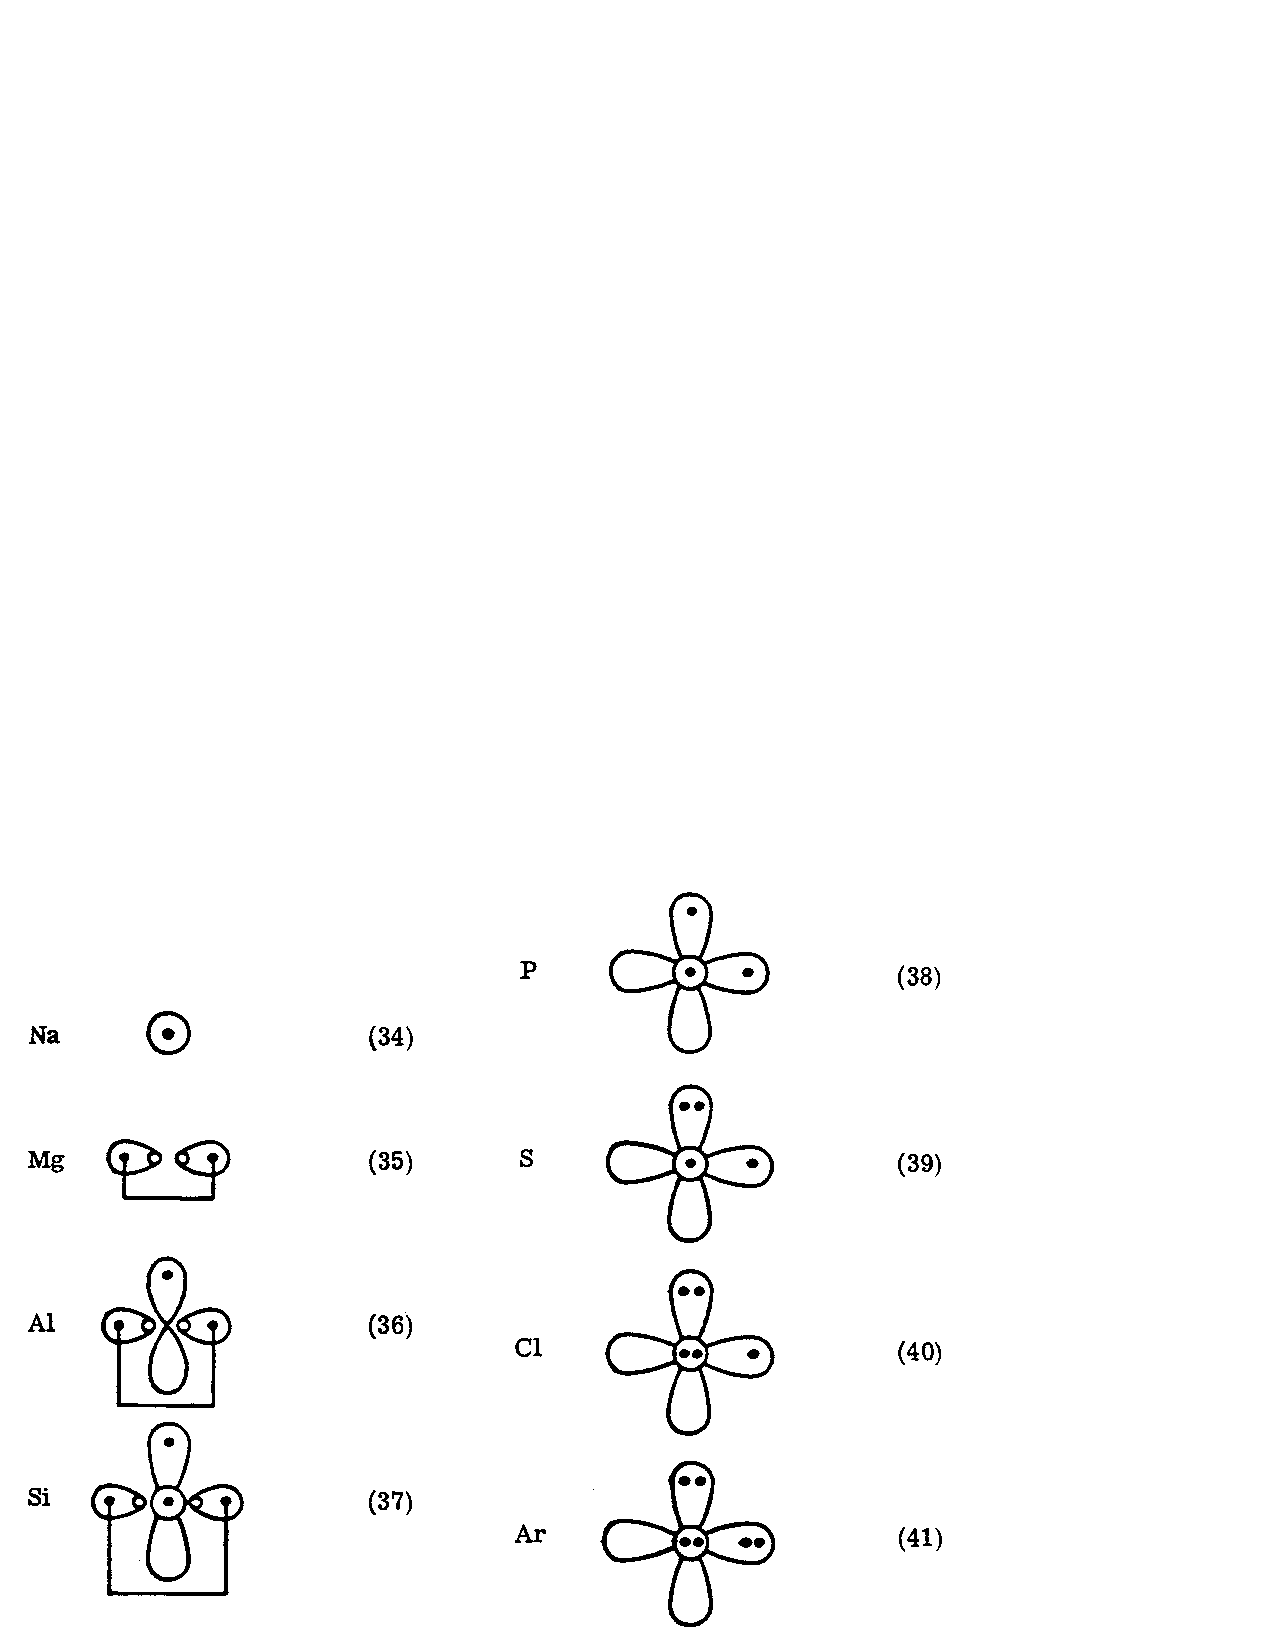
\includegraphics[scale=0.75]{fig6-06c}
\end{equation}
and combining to form wavefunctions for homonuclear diatomic 
molecules, leads to the group state configurations
\begin{equation}
%figure missing here, p 8.2-2
\end{equation}
In discussing the molecular states, we will often find it convenient 
to utilize MOs constructed as symmetry combinations of 
atomic orbitals
\begin{equation}
%figure missing here, p 8.2-4
\end{equation}
which will be analyzed in more detail in the balance of this chapter.  
The ground state configurations from Na$_2$ to Ar$_2$, are listed in 
Tables \ref{chap10-tab4a}--\ref{chap10-tab4b}.

\begin{table}
\caption{Properties of third row homonuclear diatomic 
molecules.$^a$ The first column if the number of valence electrons.}
\label{chap10-tab4a}
\begin{tabular}{cccccccc}\\ \hline

& Molecule & $R_e$ (\AA)& $\omega_e$ (cm$^{-1}$)&\multicolumn{2}{c}{$D_0$}
&\multicolumn{2}{c}{IP (eV)}\cr 
& & & &eV &kcal & molecule & atom$^b$\cr

1 & Na$^+_2$ & (3.54) & (126) & 0.96 & 22.14\cr
2 & Na$_2$ & 3.0789 & 159.1 & 0.720 & 16.60 & 4.90 & 5.138\cr
3 \cr
4 & Mg$_2$ & 3.890$^5$ & 51.1 & 0.0501 & 1.16 & & 7.644\cr
5 \cr
6 &Al$_2$ & 2.466 & 350.0 & 1.5$^5$ & 35.74 & & 5.984\cr
7 \cr
8 & Si$_2$ & 2.246 & 511.0 & 3.21 & 74.02 & & 8.149\cr
9 & P$^+_2$ & 1.985$^9$ & 672.2 & 4.99 & 115.07\cr
10 & P$_2$ & 1.8934 & 780.8 & 5.033 & 116.06 & 10.53 & 10.484\cr
11 & S$^+_2$ & (1.82$^5$) & 790 & 5.37 & 123.83\cr
12 & S$_2$ & 1.8892 & 725.7 & 4.3693 & 100.76 & 9.36 & 10.357\cr
13 & S$^-_2$ & - & 600.8 & 3.95$^5$ & 91.20 & 1.66$^3$ & 2.0772\cr
& Cl$^+_2$ & 1.8915 & 645.6 & 3.95 & 91.09\cr
14 & Cl$_2$ & 1.987$^9$ & 559.7 & 2.4794 & 57.17 & 11.50 & 13.01\cr
15 & Cl$_2$ & & & 1.26 & 29.06 & 2.39 & 3.615\cr
& Ar$^+_2$ & (2.43) & & 1.33 & 30.67\cr
16 & Ar$_2$ & 3.758 & [25.7] & 0.0105 & 0.24 & 14.54 & 15.755\cr
\hline
\end{tabular}
\end{table}


\begin{table}
\caption{MO configurations.}
\label{chap10-tab4b}

\begin{tabular}{ccccccccc}\\ \hline
& Molecule & Symmetry & $\sigma_g3s$ & $\sigma_u3s$ & $\sigma_g 
3p$ & $\pi_u3p$ & $\pi_g3p$ & $\sigma_u3p$\cr

1 & Na$^+_2$ & ${^2\Sigma}^+_g$ & 1 & 0 & 0 & 0 & 0 & 0\cr
2 & Na$_2$ & ${^1\Sigma}^+_g$ & 2 & 0 & 0 & 0 & 0 & 0\cr 
3 &\cr
4 & Mg$_2$ & ${^1\Sigma}^+_g$ & 2 & 2 & 0 & 0 & 0 & 0\cr 
5 &\cr
6 &Al$_2$ & ${^3\Sigma}^-_g$ & 2 & 2 & 0 & 2 & 0 & 0\cr 
7 &\cr
8 & Si$_2$ & ${^3\Sigma}^-_g$ & 2 & 2 & 2 & 2 & 0 & 0\cr 
9 & P$^+_2$ & ${^1\Pi}_{ui}$ & 2 & 2 & 2 & 2 & 3 & 0\cr
10 & P$_2$ & ${^1\Sigma}^+_g$ & 2 & 2 & 2 & 4 & 0 & 0\cr
11 & S$^+_2$ & ${^2\Pi}_{gr}$ & 2 & 2 & 2 & 4 & 1 & 0\cr  
12 & S$_2$ & ${^3\Sigma}^-_g$ & 2 & 2 & 2 & 4 & 2 & 0\cr
13 & S$^-_2$ & ${^2\Pi}_{gi}$ & 2 & 2 & 2 & 4 & 3 & 0\cr 
& Cl$^+_2$ & ${^2\Pi}_{gi}$ & 2 & 2 & 2 & 4 & 3 & 0\cr
14 & Cl$_2$ & ${^1\Sigma}^+_g$ & 2 & 2 & 2 & 4 & 3 & 0\cr
15 & Cl$_2$ & ${^2\Sigma}^+_u$ & 2 & 2 & 2 & 4 & 4 & 1\cr
& Ar$^+_2$ & & 2 & 2 & 2 & 4 & 4 & 1\cr
16 & Ar$_2$ & ${^1\Sigma}^+_g$ & 2 & 2 & 2 & 4 & 4 & 2\cr
\hline
\end{tabular}\\
$^a$ See reference 1.  Unless stated otherwise, all experimental data 
on diatomic molecules in this chapter are from this reference.
$^b$ Table \ref{chap5-table5} of Chapter 5.
$^c$ The subscript $r$ or $i$ indicates a less than 
half-filled, $r$ for regular, or more than half-filled, 
$i$ for inverted, shell with $\lambda \not= 0$.
$^d$ $D_0(AB)$ is the energy difference between separated atoms A 
and B, and the lowest, $v$, vibrational level of the molecule, $v = 0$.
\end{table}


\subsection{Na$_2$}

Except for the presence of the two Ne cores, the wavefunctions for 
Na$_2$
\begin{equation}
\left( \phi_{3sl} \phi_{3sr} + \phi_{3sr} \phi_{3sl} \right) \left( 
\alpha \beta - \beta \alpha \right)
\end{equation}
and Na$^+_2$
\begin{equation}
\left( \phi_{3sl} + \phi_{3sr} \right) \alpha
\end{equation}
are quite analogous to those of H$_2$ and H$_2^+$.  These core 
orbitals will be ignored in all wavefunctions.  In MO 
language, the wavefunction for Na$_2$ is
\begin{equation}
\phi_{\sigma_g 3s} \phi_{\sigma_g3s} ( \alpha \beta - \beta \alpha )
\end{equation}
and for Na$_2^+$ is
\begin{equation}
\phi_{\sigma_g3s}\alpha
\end{equation}
where
\begin{equation}
\phi_{\sigma_g3s} = \phi_{3sl} + \phi_{3sr}.
\end{equation}
Since H$_2$ is considerably more strongly bound than H$^+_2$ (there being two
electrons in the bonding orbital rather than one) it is surprising 
to find that Na$_2$ is more \emph{weakly} bound than Na$^+_2$, and the same for 
other alkali diatomics. The origin of this effect will be explained 
later.

\subsection{Mg$_2$}

In order to make a bond between Mg atoms, we must unpair the lobe 
pairs of orbitals on each atom
\begin{equation}
% figure missing p 8.2-5
%\includegraphics
\end{equation}
The net result is a very weak bond, 
\begin{equation}
D_0 ( {\rm Mg}_2) = 0.05 {\rm eV} = 1.15~{\rm kcal}.
\end{equation}
At large distances, the overlap of the lobe orbitals is too small to unpair 
the orbitals on each atom.  The result is a potential curve with a small 
hump, and a small minimum, as shown in Figure \ref{chap10-fig4}.

\begin{figure}
% fig 4 not foudn (p 8.2-6)
%\includegraphics[scale=0.75]{fg10-}
\caption{}
\label{chap10-fig4}
\end{figure}

We saw a bonding and a nonbonding pair:
\begin{equation}
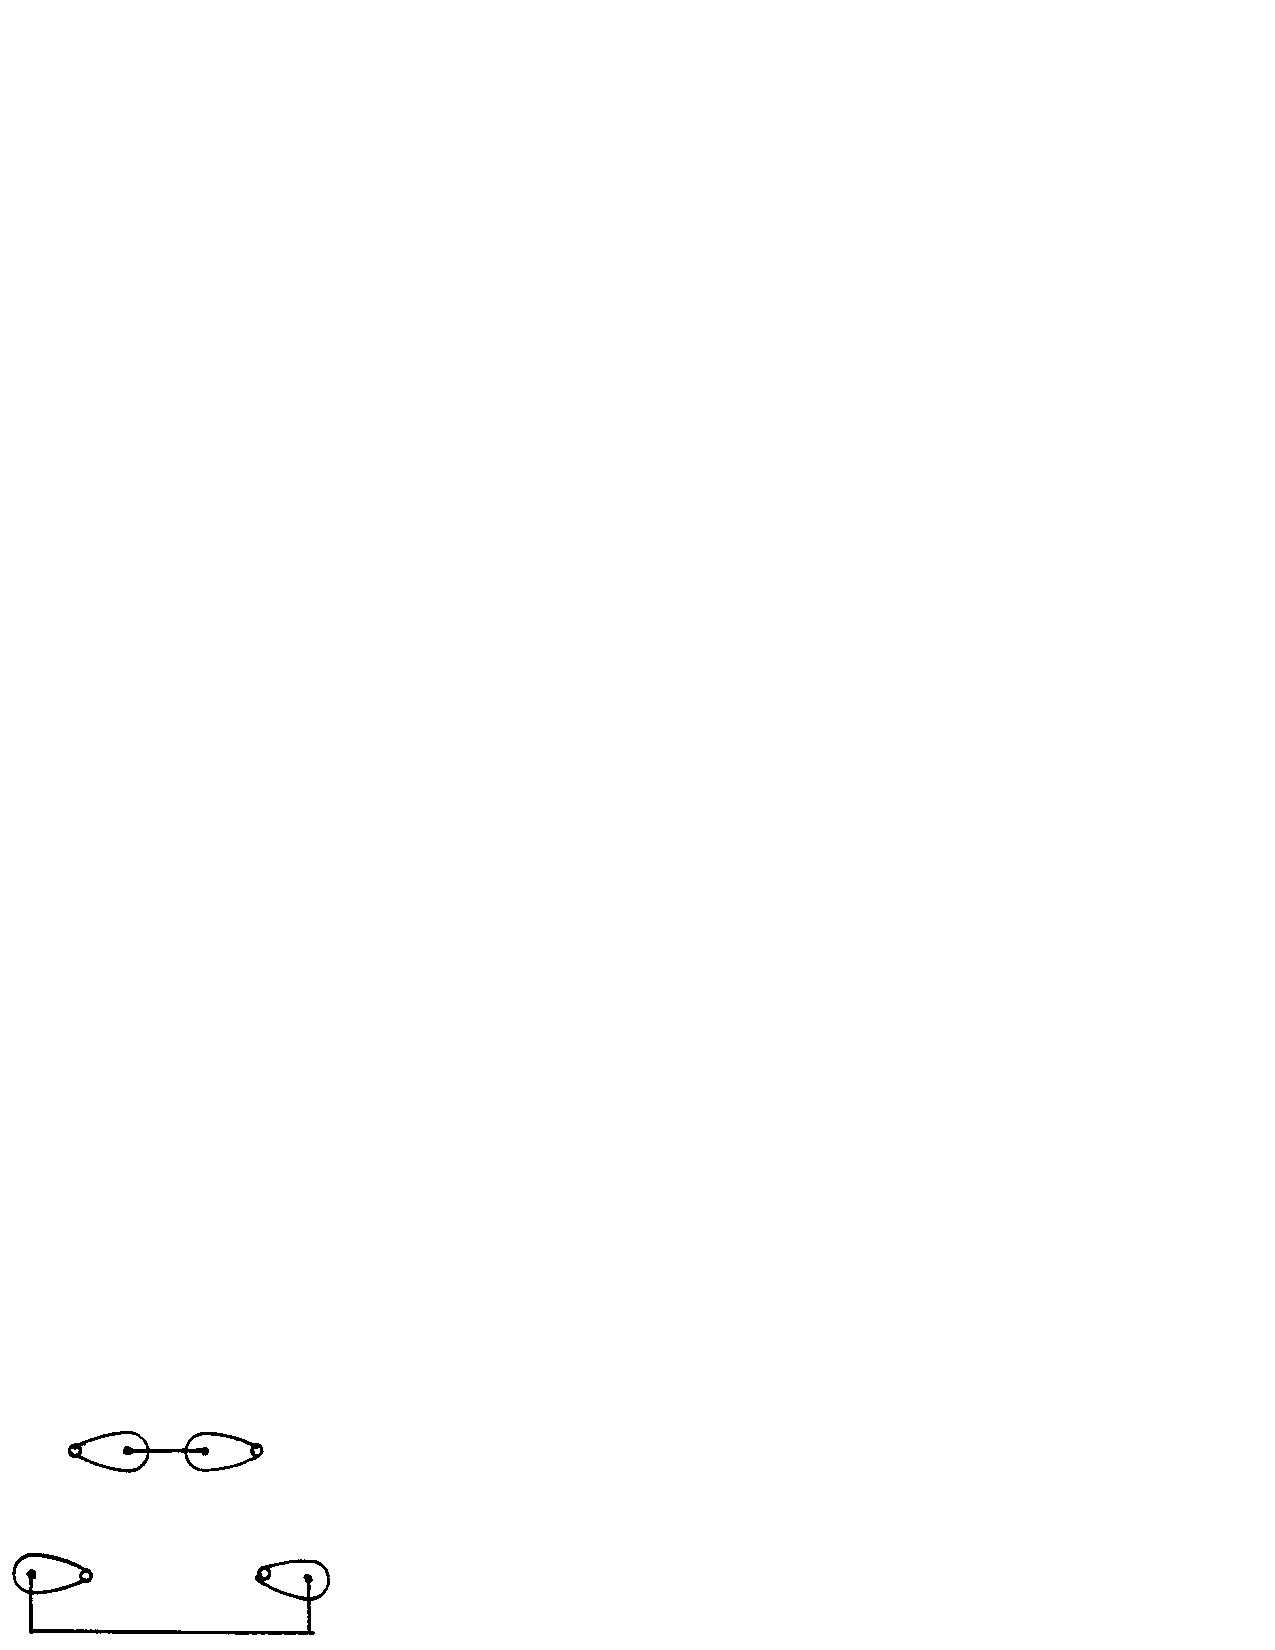
\includegraphics{fg10-4a}
\end{equation}
Since the net bond is almost negligible, we can consider the second 
pair as an antibond equal in strength to the bond.

In the MO description, the configuration for Mg$_2$ is
\begin{equation}
\left( \sigma_g 3s \right)^2 \left( \sigma_u 3s \right)^2.
\end{equation}
Thus, with two electrons in the bonding orbital, $\sigma_g 3s$, and two 
electrons in the antibonding orbital, $\sigma_u 3s$ it is expected that 
Mg$_2$ is not
bound.  On the other hand, Mg$_2^+$, with only one electron in the 
$\sigma_u 3s$ orbital should be strongly bound, as indicated in Figure 
\ref{chap10-fig4}.

\subsection{P$_2$}

We will skip Al$_2$ and Si$_2$ for now, and consider P$_2$.  As indicated in
\begin{equation}
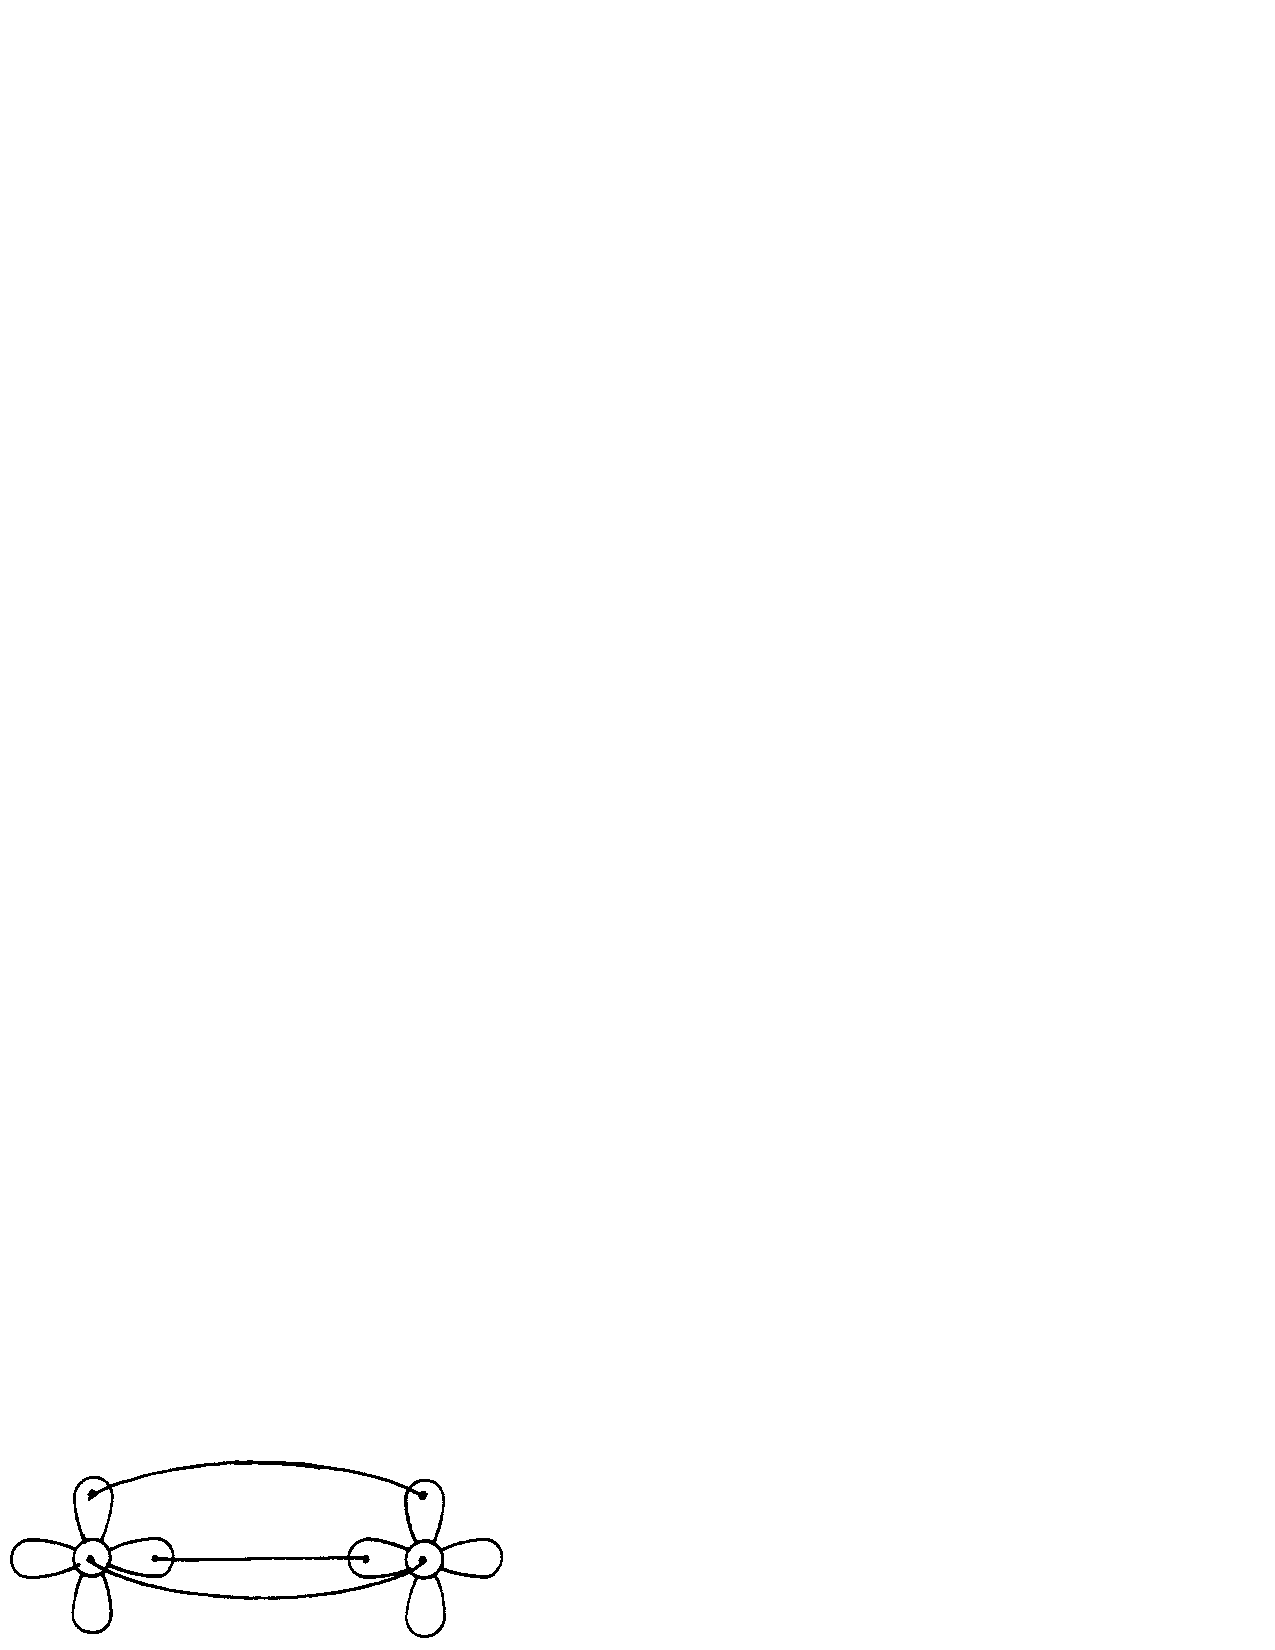
\includegraphics{fg10-4b}
\end{equation}
we can form three two-electron bonds, one $\sigma$ bond, and two $\pi$ 
bonds.  As a result, the bond energy of P$_2$ is quite high,
\begin{equation}
D_0 ({\rm P}_2) = 5.03 {\rm eV} = 116.1 {\rm kcal}.
\end{equation}

In MO language, the three bonding orbitals are $\sigma_g3p$ (top
pair), $\pi_u 3p_x$ (bottom pair), and $\pi_u 3p_y$ (bottom pair, but
rotated out of the plane):
\begin{equation}
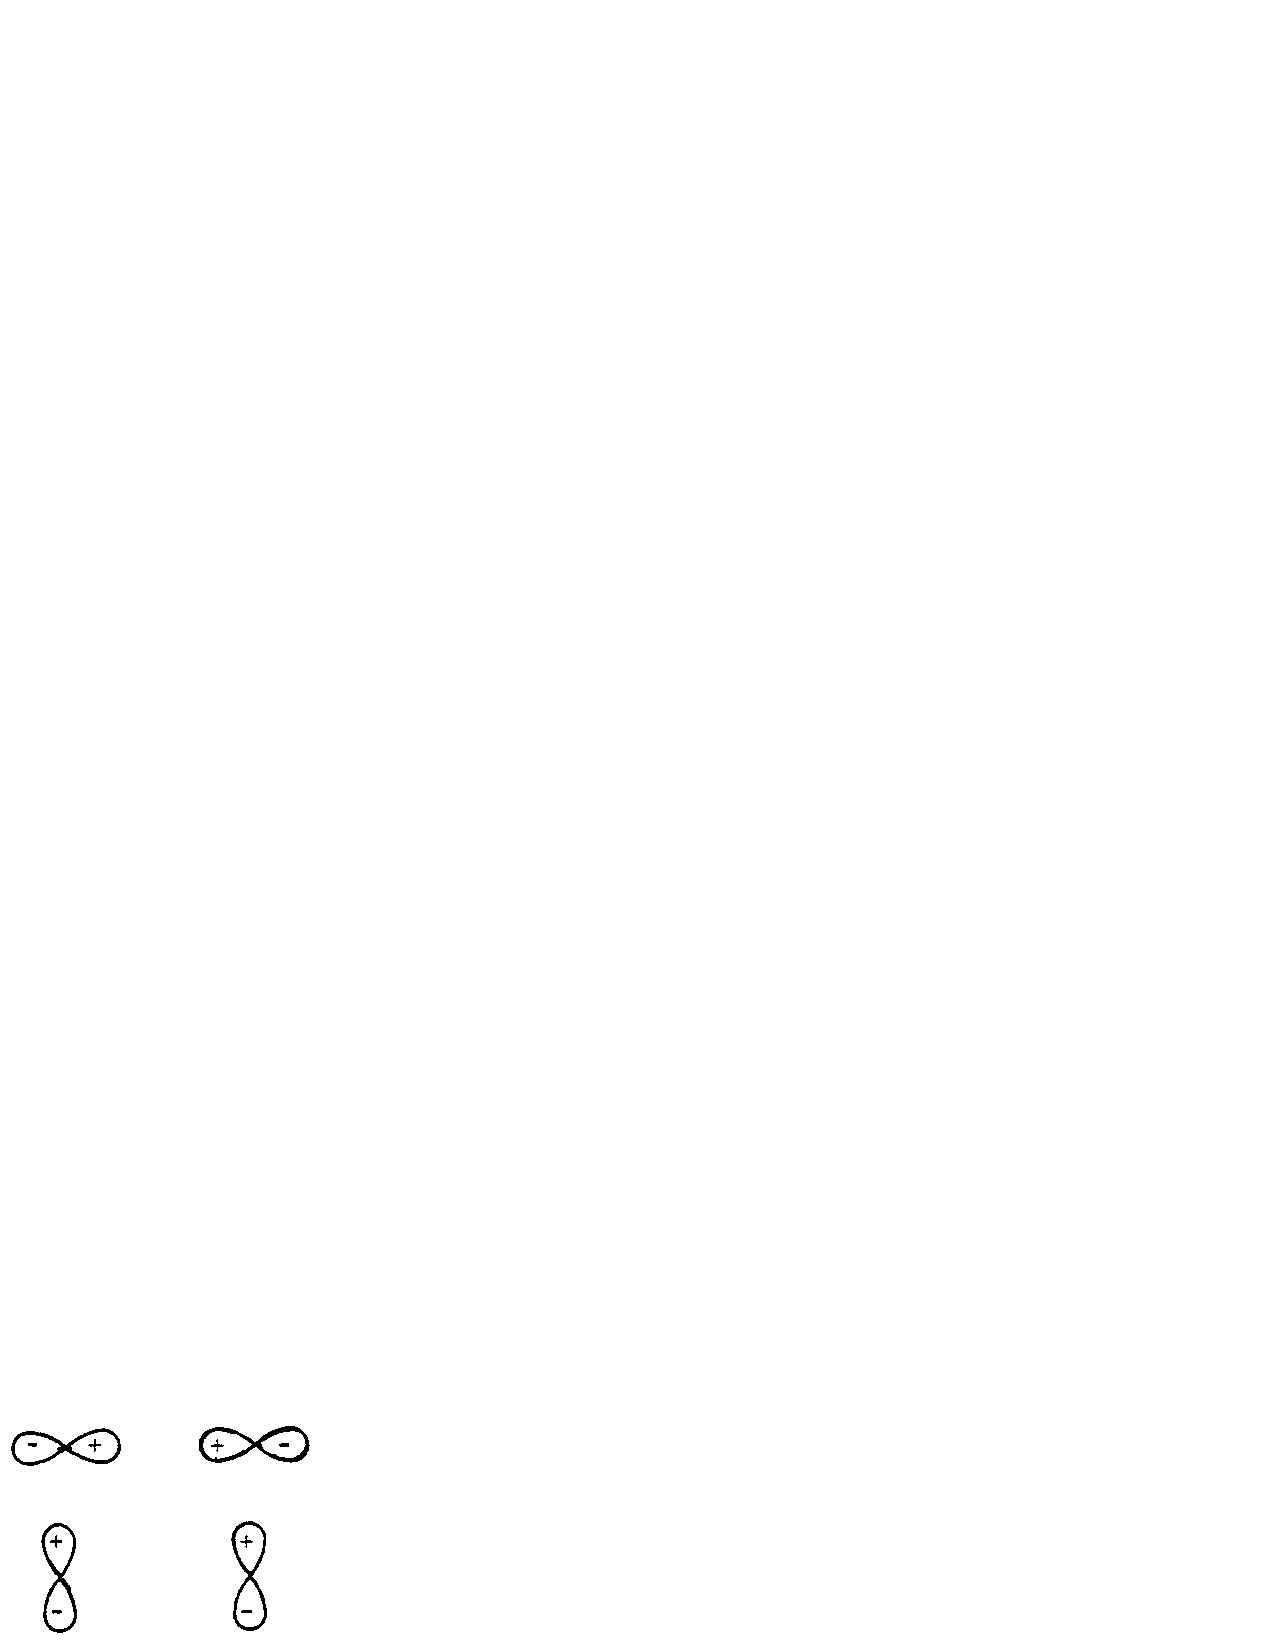
\includegraphics{fg10-4c}
\end{equation}
so that the total valence configuration is
\begin{equation}\left( \sigma_g 3s \right)(^2 \left( \sigma_u 3s
\right)^2 \left(\sigma_g 3p \right)^2 \left( \sigma_u 3p \right)^2.
\end{equation}
Since all occupied orbital shells are completely filled, closed shell,
the total symmetry is ${^1\Sigma}^+_g$.

The $\pi$ bond is expected to be weaker than the $\sigma$ bond, lower overlap, 
and hence, the lowest ionization of P$_2$ should be from the $\pi_u 
3p$ orbital, leading
to a ${^2\Pi}_u$ state for P$_2^+$.  Since the $\pi_u3p$ orbital is bonding, we 
expect for P$^+_2$ a larger $R_e$, a smaller 
vibrational frequency, $\omega_e$, and a weaker bond.
These expectations are correct,
\begin{equation}
\begin{array}{lcc} \\
& \mathrm{P}_2 & \mathrm{P}_2^+\\
R_e ( {\rm \AA} ) & 1.8934& 1.9859\cr
\omega_e ( {\rm cm}^{-1} ) & 780.8 & 672.2\cr
D_0 ( {\rm kcal} ) & 116.1& 115.1
\end{array}
\end{equation}
although the bond is not weakened much.

\subsection{S$_2$}

For S$_2$, the favorable bonding configurations are
\begin{equation}
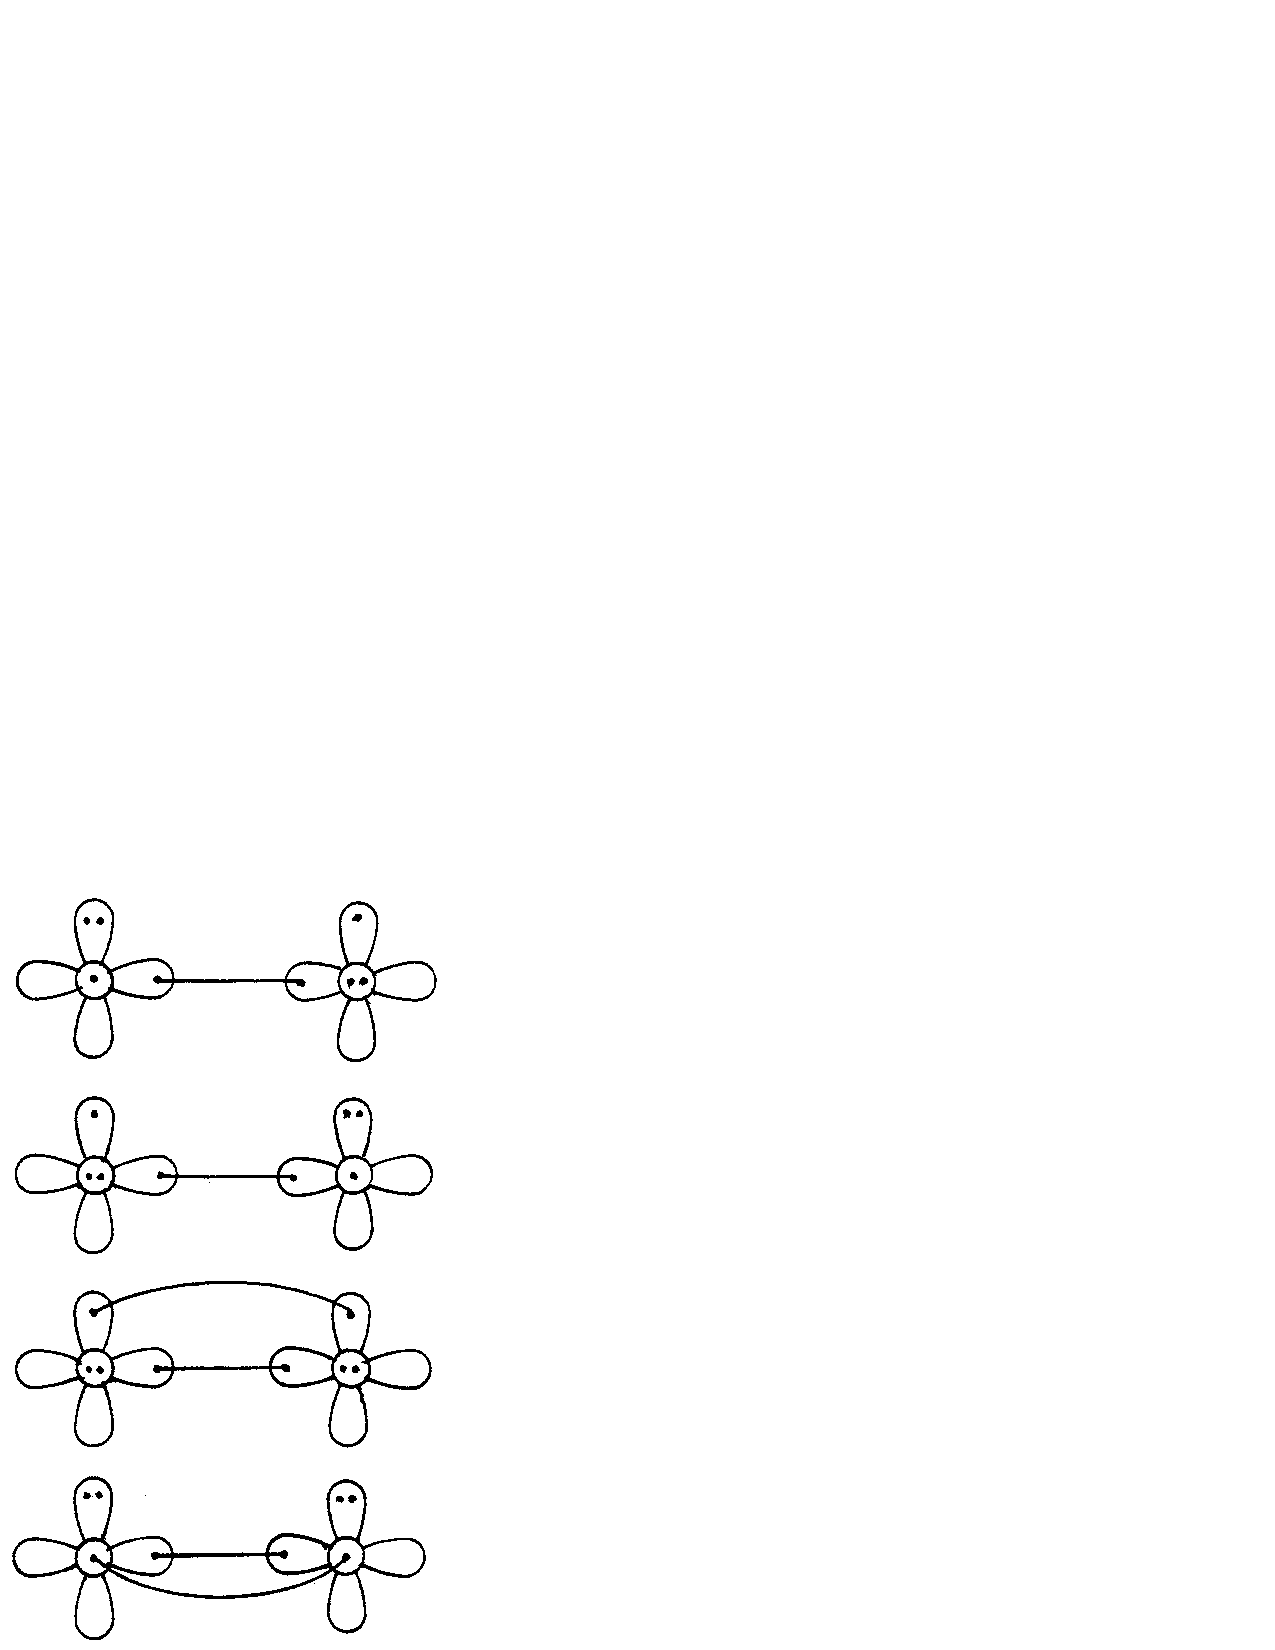
\includegraphics{fg10-4d}
\label{chap10-eqno24}
\end{equation}
all of which correspond to the MO configuration of
\begin{equation}
\left( \sigma_g 3s \right)^2 \left( \sigma_u 3s \right)^2 \left( \sigma_g 
3sp \right)^2 \left( \pi_u 3p  \right)^4 \left( \pi_g 3p \right)^2 
.
\label{chap10-eqno25}
\end{equation}
Compared to P$_2$ we have added two electrons to antibonding $\pi_g3p$ orbitals
\begin{equation}
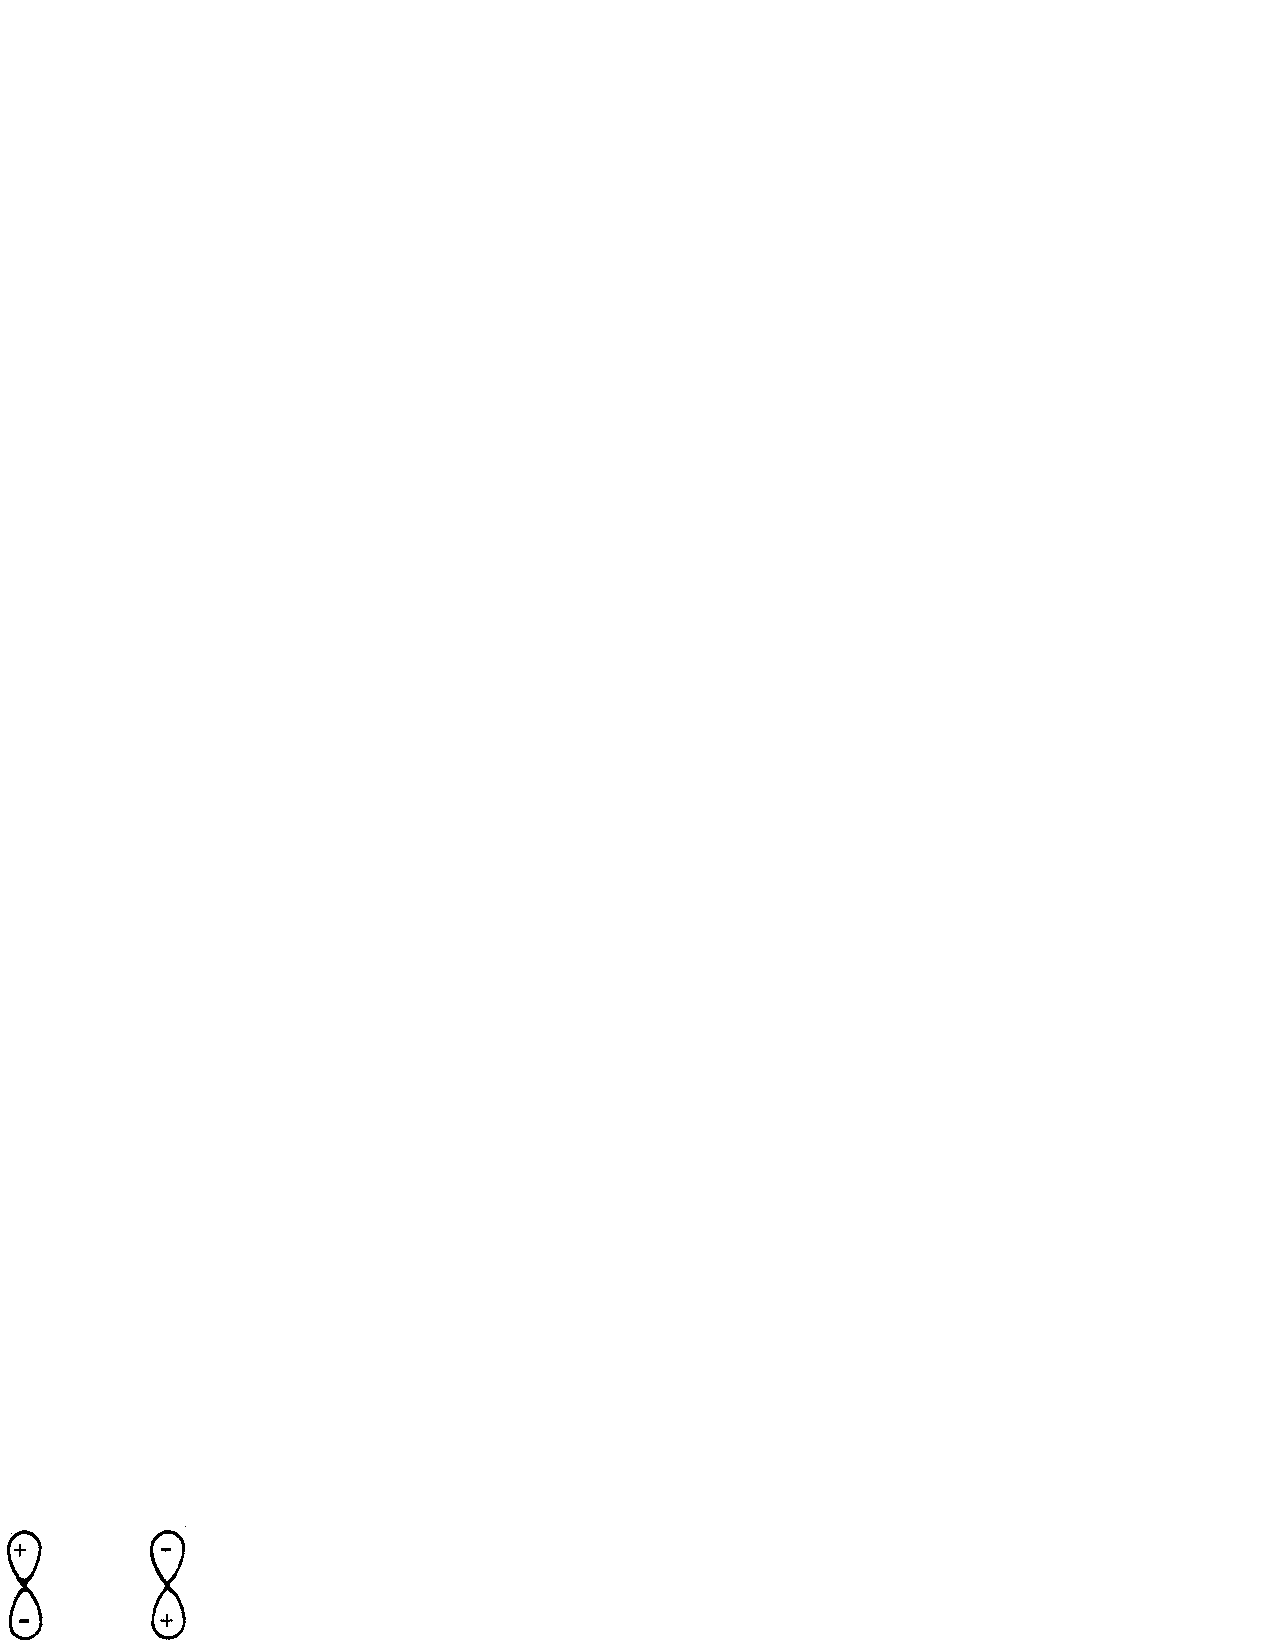
\includegraphics{fg10-4e}
\end{equation}
and indeed the bond in S$_2$ is 100.8 kcal as compared to 116.1 kcal for 
P$_2$.

As discussed, a $\pi^2_g$ configuration leads to three states
where the separation between states is $2K_{xy}$.  For S$_2$, the relative 
energies are shown in Figure \ref{chap10-fig5}, where we see that
\begin{equation}
K_{xy} \approx 0.29~{\rm eV} .
\end{equation}

\begin{figure}
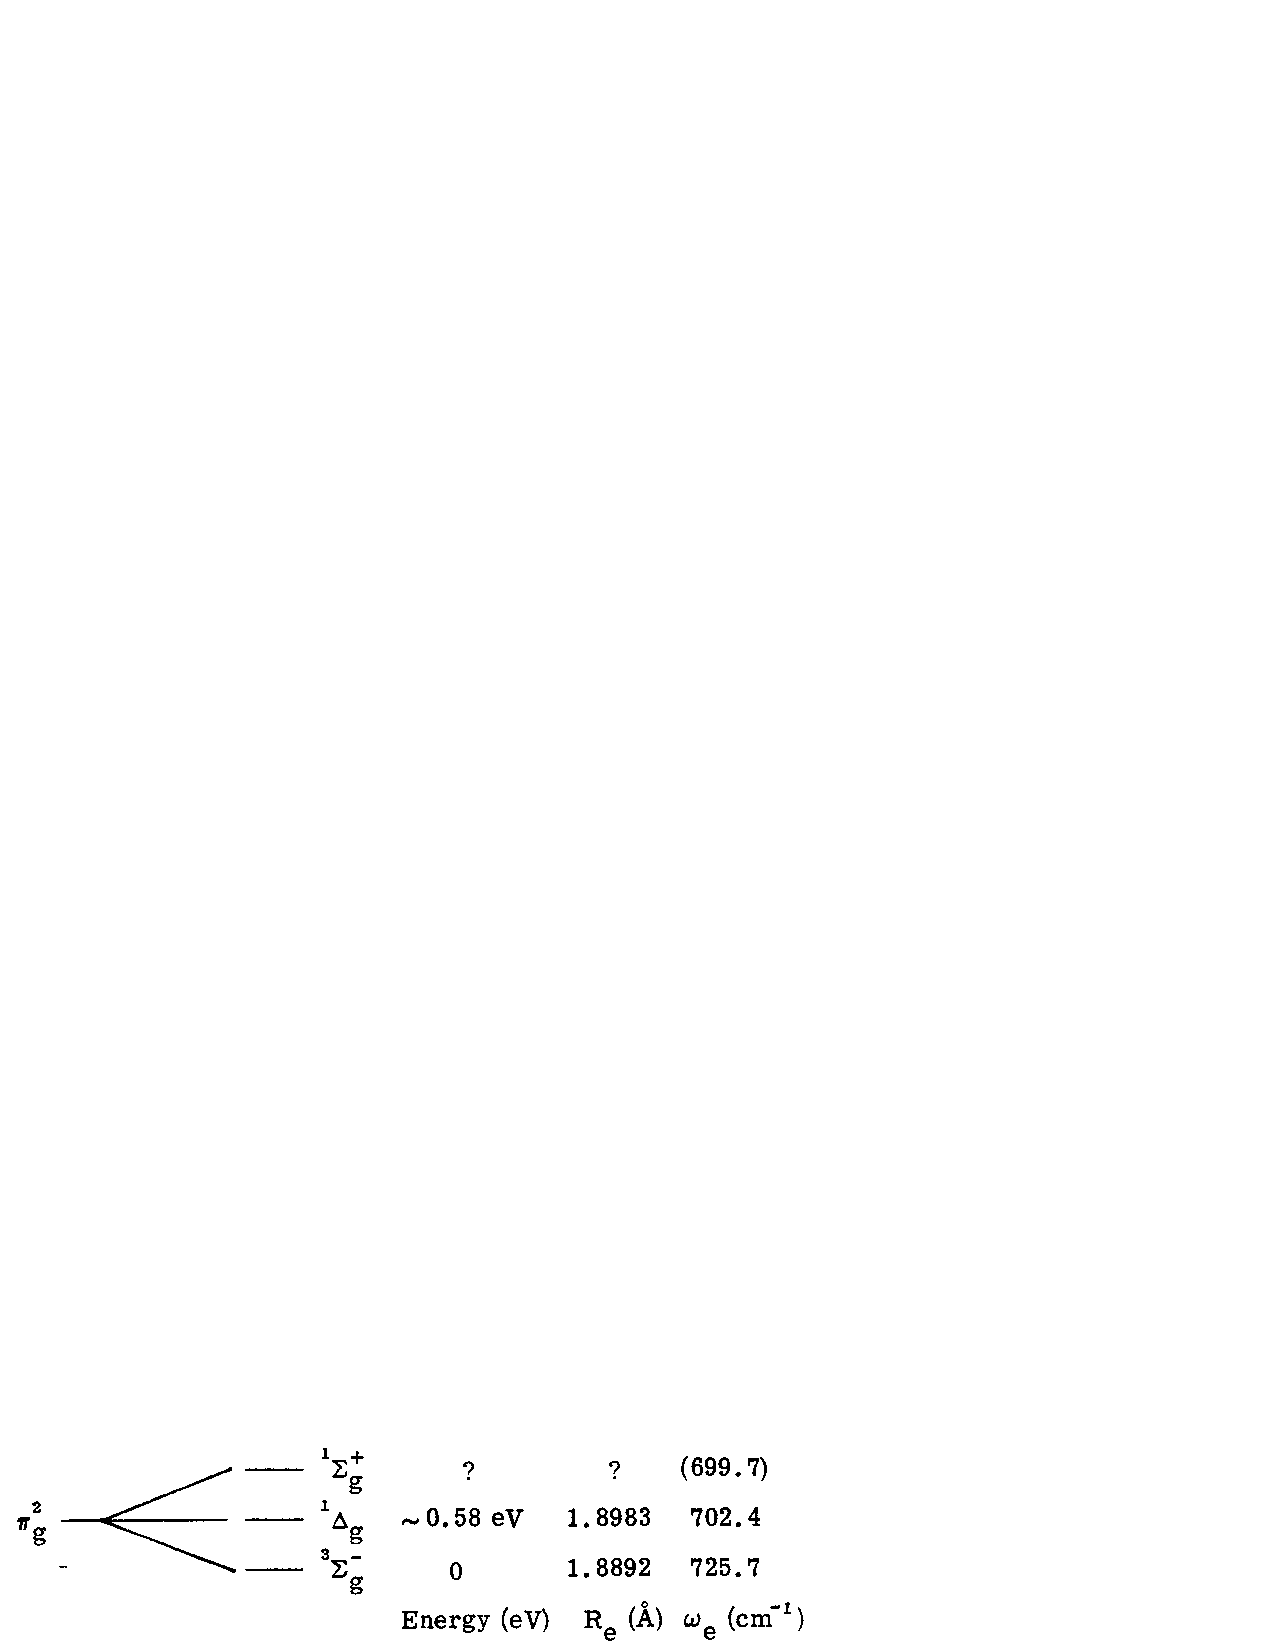
\includegraphics[scale=0.75]{fg10-5}
\caption{}
\label{chap10-fig5}
\end{figure}

The two diagrams in equation (\ref{chap10-eqno24}) are equivalent in
energy but interact strongly, leading to a final wavefunction of the
form
\begin{equation}
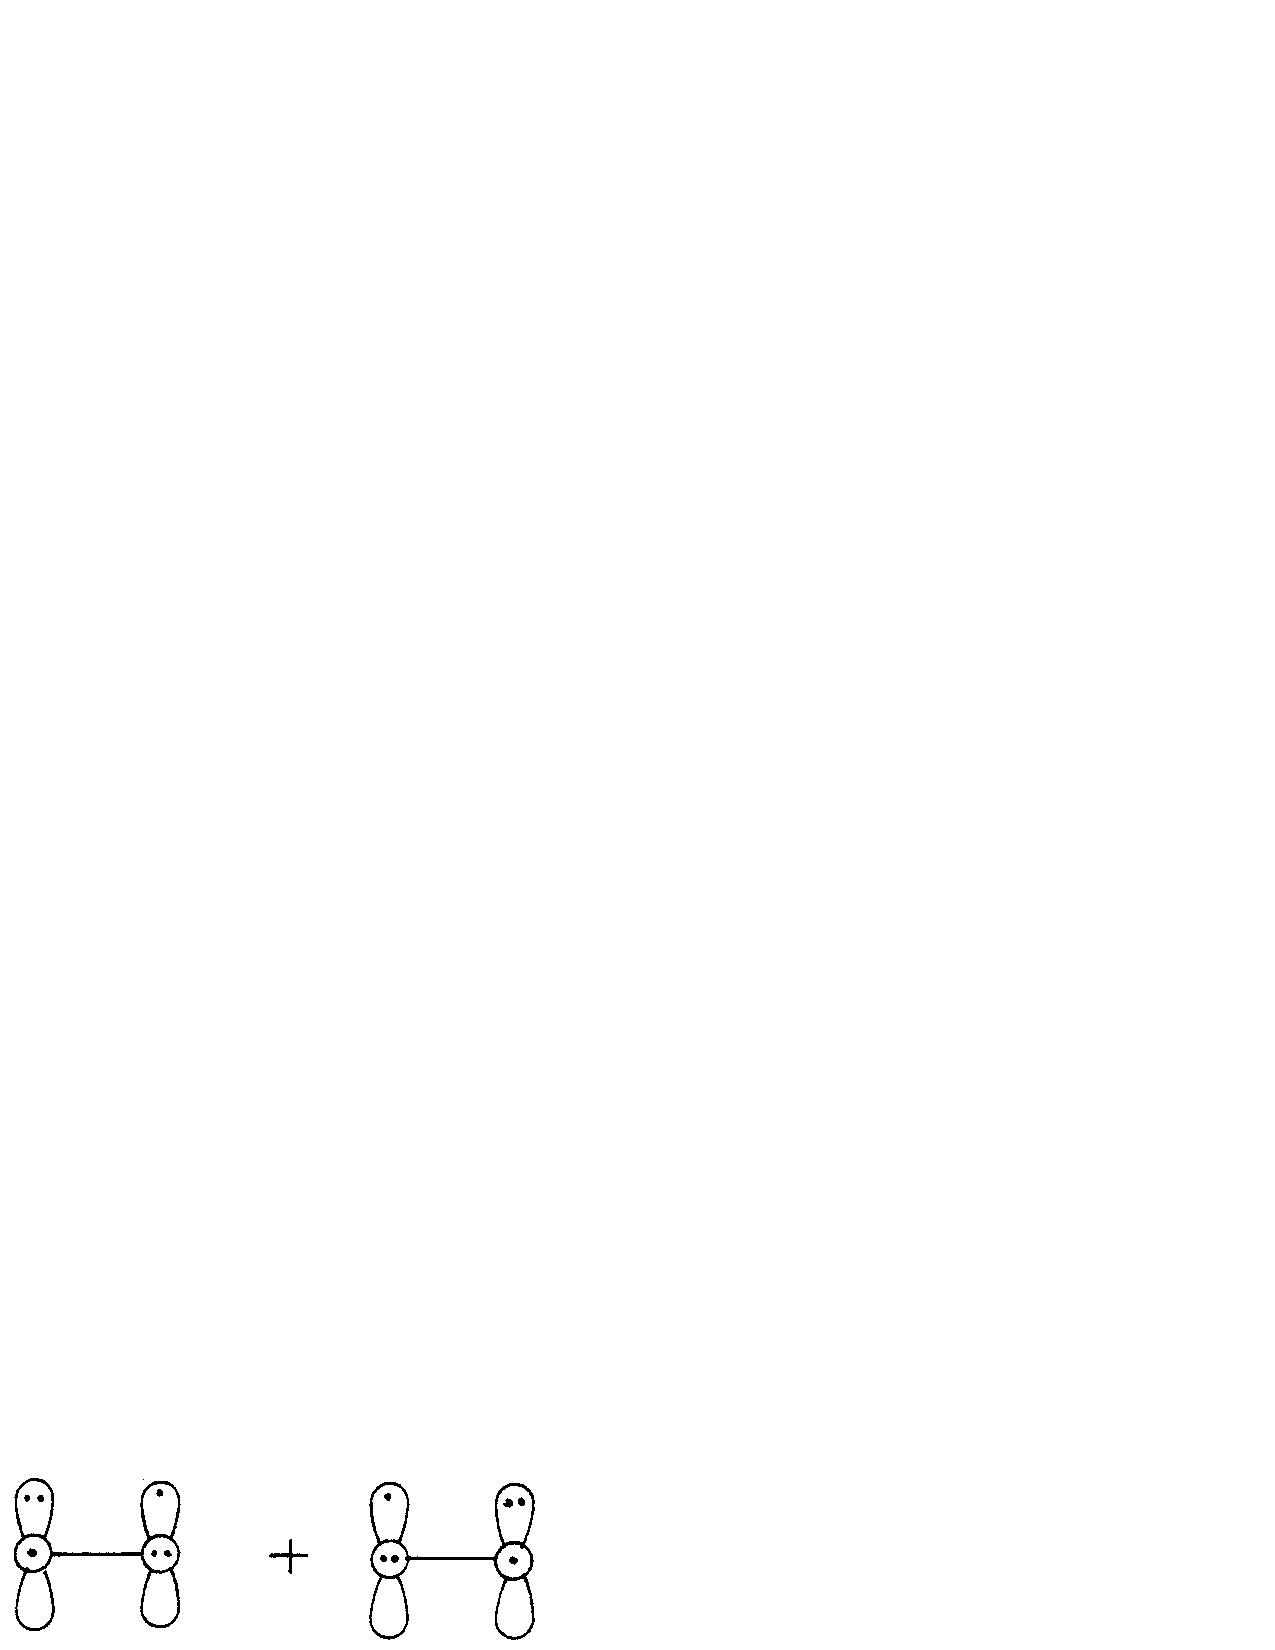
\includegraphics{fg10-5a}
\label{chap10-eqno26}
\end{equation}
This leads to ${^3\Sigma}^-_g$, for ${^1\Delta}^-_g$, depending upon
the spin coupling of the two singly occupied orbitals.  Similarly, the
other two diagrams in equation (\ref{chap10-eqno24}) interact, leading
to
\begin{equation}
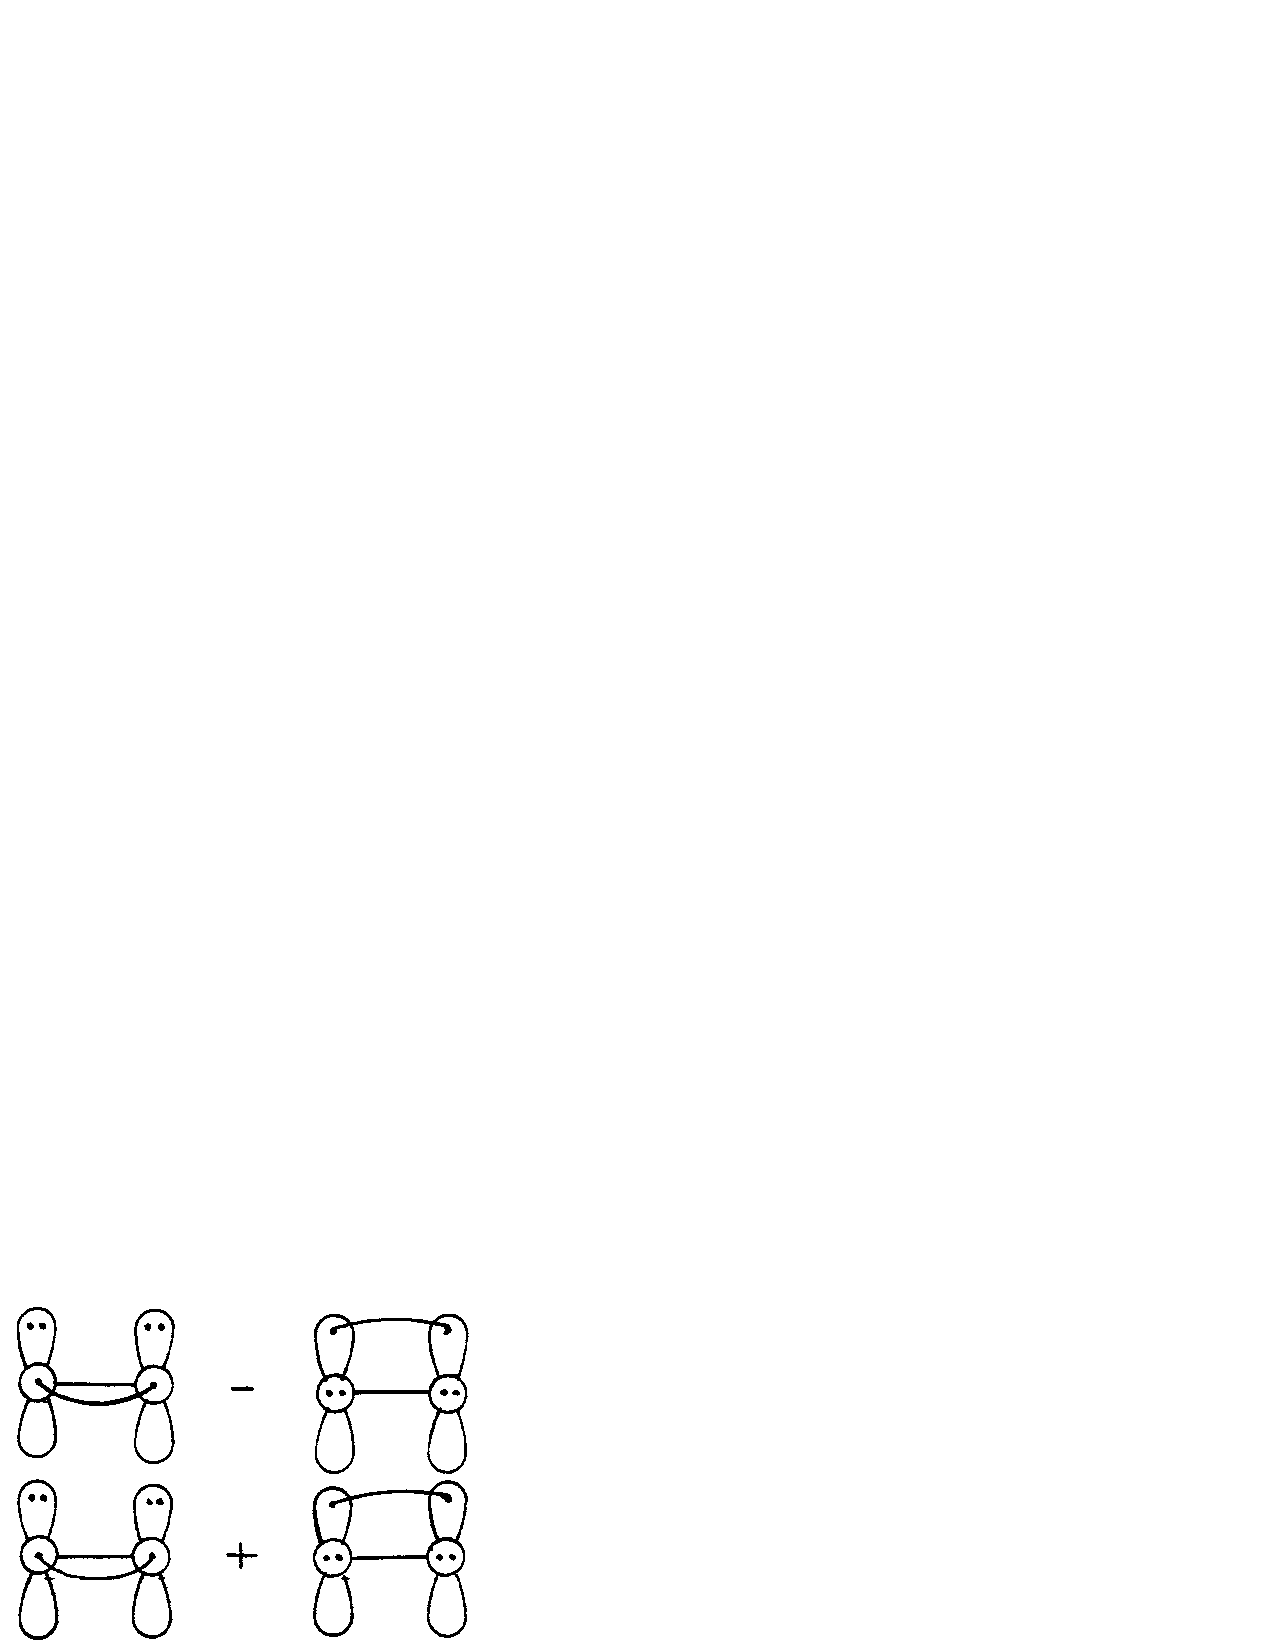
\includegraphics{fg10-5b}
\end{equation}

From the MO configuration in equation (\ref{chap10-eqno25}), we expect 
that the ground states of S$^+_2$ and S$^-_2$ 
differ only by the occupation of the $\pi_g3p$ orbital
\begin{eqnarray}
S^+_2 &:& \left( \pi_g 3p \right)^1 \rightarrow {^2\Pi}_g\cr
S_2  &:& \left( \pi_g 3p \right)^2 \rightarrow {^2\Sigma}^-_g , {^1\Delta}_g , 
{^1\Sigma}^+_g\cr
S^-_2 &:& \left( \pi_g 3p \right)^2 \rightarrow {^2\Pi}_g
\end{eqnarray}
Since this orbital is antibonding, the bond length should increase and
the bond energy should decrease as electrons are added to $\pi_g3p$.
Indeed, these trends are observed in Table \ref{chap10-tab5}.

\begin{table}
\caption{}
\label{chap10-tab5}
\begin{tabular}{ccccc}\\ \hline
& State & $R_e$ (\AA) & $\omega_e$ (cm$^{-1}$) & $D_e$ (kcal)\cr
S$^+_2$ & ${^2\Pi}_g$ & (1.825) & 790 & 123.8\cr
S$_2$ & ${^3\Sigma}^-_g$ & 1.8892 & 725.7 & 100.8\cr
S$^+_2$ & ${^2\Pi}_g$ & & 600.8 & 91.2\cr
\hline
\end{tabular}
\end{table}


\subsection{Cl$_2$}

For Cl$_2$, the valence bond bonding configuration is
\begin{equation}
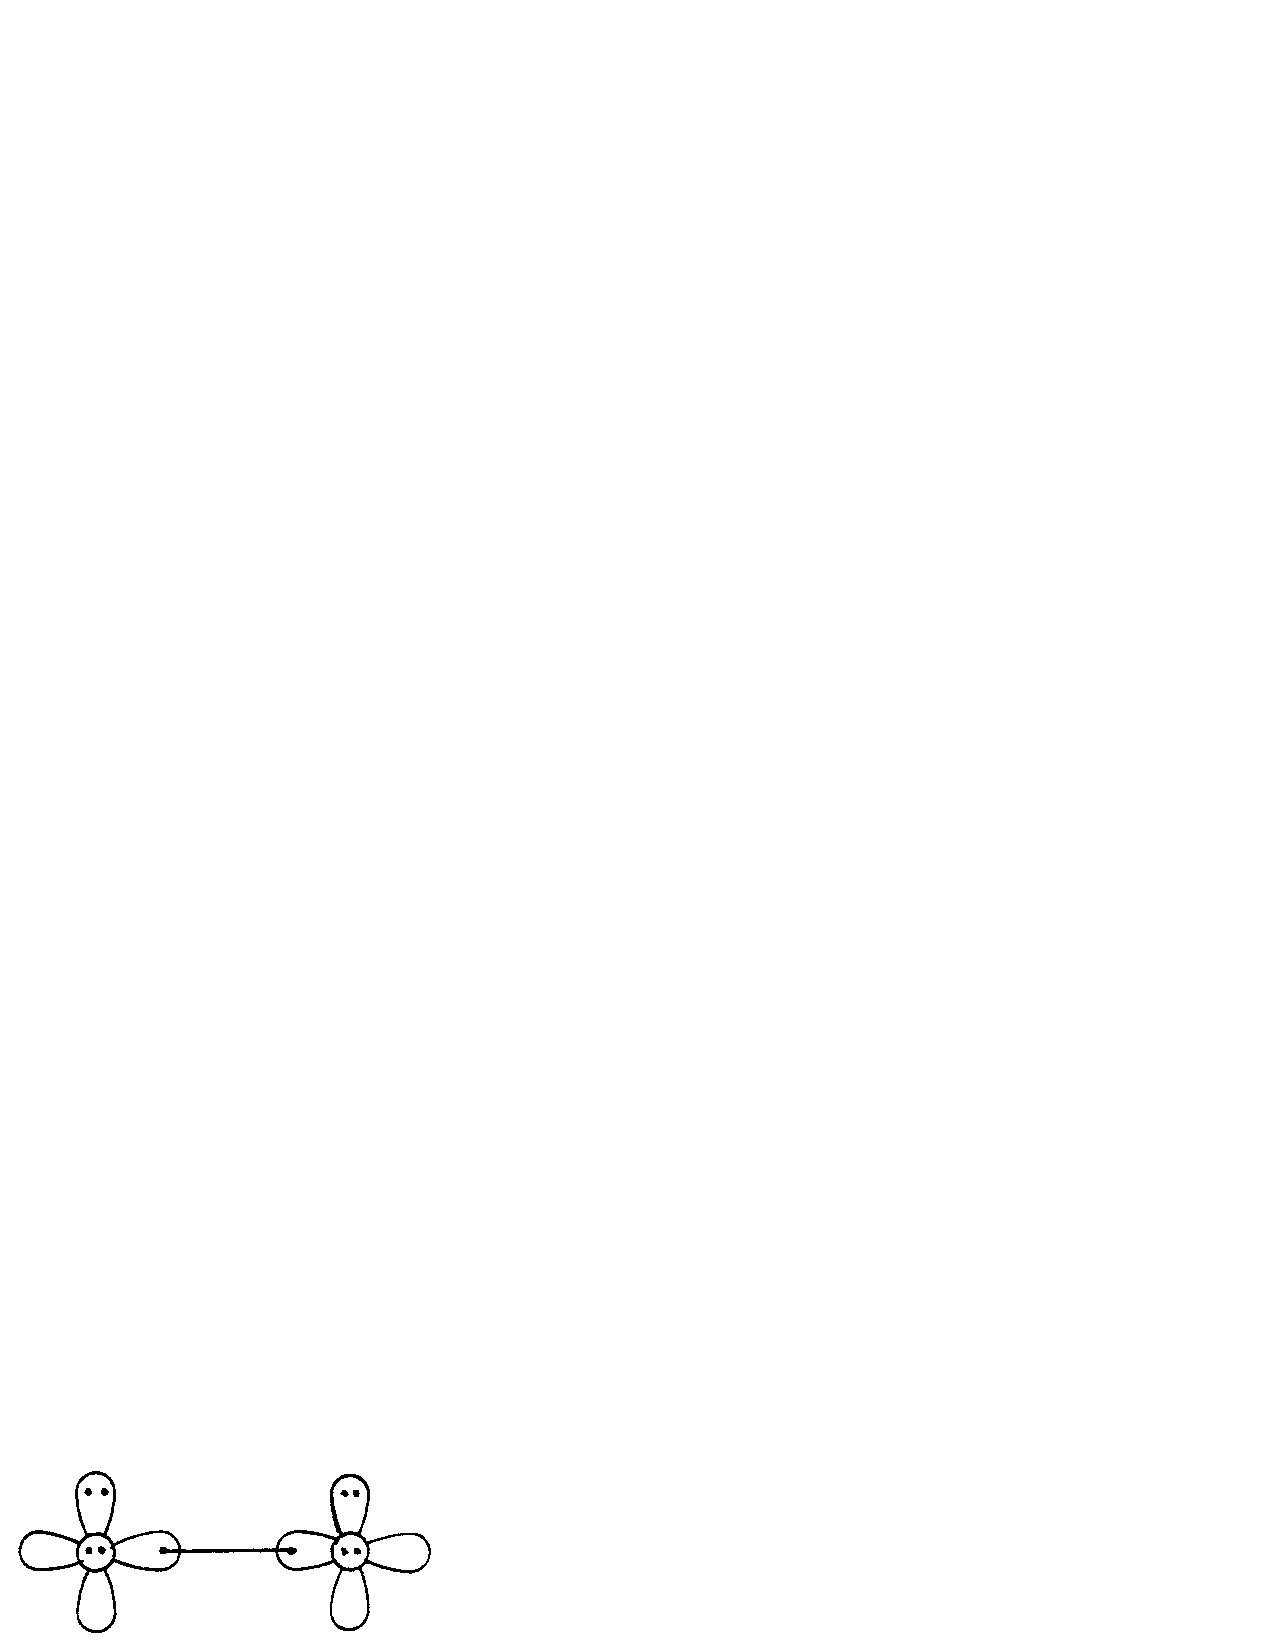
\includegraphics{fg10-5c}
\end{equation}
and the MO valence configuration is
\begin{equation}
\left( \sigma_g 3s \right)^2 \left( \sigma_u 3s \right)^2 \left( 
\sigma_g 3p \right)^2 \left( \pi_u 3p \right)^4 \left( \pi_g 3p 
\right)^4 .
\label{chap10-eqno27}
\end{equation}
leading to a ${^1\Sigma}^+_g$ state, closed shells.  From equation
(\ref{chap10-eqno27}), the ground state of Cl$^+_2$ is obtained by
removing one electron from a $\pi_g3p$, antibonding orbital, leading
to a ${^2\Pi}_g$ state.  While the ground state of Cl$^-_2$ is
obtained by adding one electron to a $\sigma_g 3p$, antibonding,
orbital, leading to a ${^2\Sigma}^+_2$ state.  Indeed, the bond
energies are generally consistent with the description shown in Table
\ref{chap10-tab6}.

\begin{table}
\caption{}
\label{chap10-tab6}
\begin{tabular}{cccccc}\\ \hline
& State & Configuration& $R_e$ (\AA)& $\omega_e$ (cm$^{-1}$)& $D_e$ (kcal)\cr
Cl$^+_2$ & ${^2\Pi}_g$ & $(\pi_g 3p)^3$ & 1.8915 & 645.6 & 91.1\cr
Cl$_2$ & ${^2\Sigma}^+_g$ & $(\pi_g 3p)^4$ & 1.9879 & 559.7 & 57.2\cr 
Cl$^-_2$ & ${^2\Sigma}^+_u$ & $(\pi_g 3p)^4(\sigma_u 3p)^1$ & & & 
29.1\cr
\hline
\end{tabular}
\end{table}


In the valence bond description, Cl$^+_2$ is described as
\begin{equation}
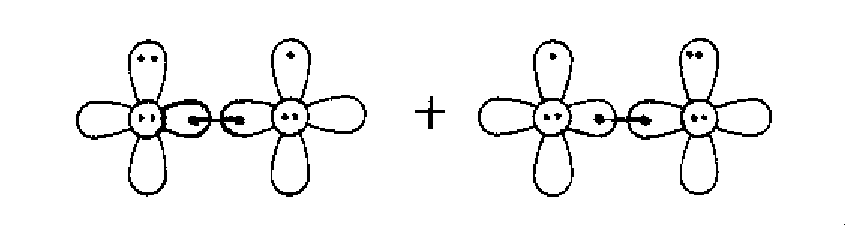
\includegraphics{fg10-5d1}
\end{equation}
Thus, there is a two-electron $\sigma$ bond and a three-electron $\pi$ 
bond.  Similarly, Cl$^-_2$ is described as
\begin{equation}
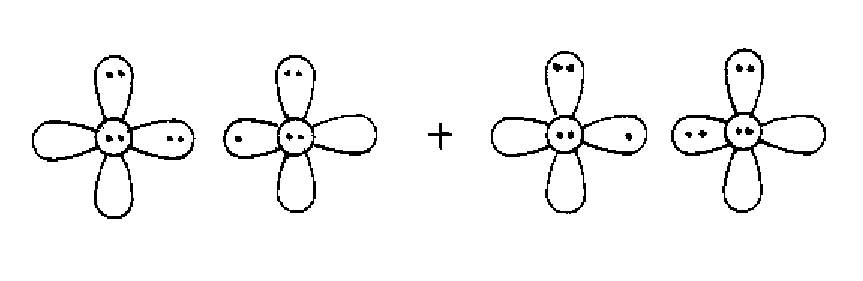
\includegraphics{fg10-5d2}
\label{chap10-eqno28}
\end{equation}
leading to a three-electron $\sigma$ bond and no $\pi$ bond.

\subsection{Ar$_2$}

For Ar$_2$, the valence bond bonding configuration is
\begin{equation}
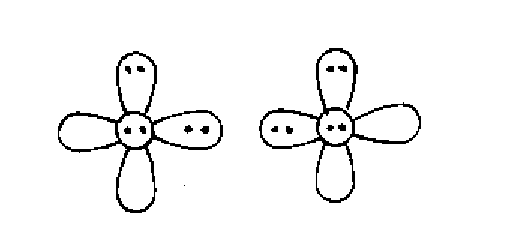
\includegraphics{fg10-5d3}
\end{equation}
and the MO valence configuration is
\begin{equation}
\left( \sigma_g 3s \right)^2 \left( \sigma_u 3s \right)^2 \left( 
\sigma_g 3p \right)^2 \left( \pi_u 3p \right)^4 \left( \pi_g 3p 
\right)^4 \left( \sigma_u 3p \right)^2
\end{equation}
leading to no net bond.  However, for Ar$^+_2$, we remove an
antibonding $\sigma_u 3p$ electron, leading to a three-electron bond
as in equation (\ref{chap10-eqno28}).  (See Table \ref{chap10-tab7}.)
Just as for He$_2$, closed-shell atoms such as Ar have very small
attractive interactions, referred to as van der Waals forces that lead
to a very weak, 0.2 kcal, very long, 3.8 \AA, bond.

\begin{table}
\caption{}
\label{chap10-tab7}

\begin{tabular}{cccccc}\\ \hline
& State & Configuration& $R_e$ (\AA)& $\omega_e$ (cm$^{-1}$)& $D_e$ (kcal)\cr
Ar$^+_2$ & ${^2\Sigma}^+_u$ & $(\sigma_u 3p)^1$ & (2.43) & - & 30.7\cr
Ar$_2$ & ${^1\Sigma}^+_g$ & $(\sigma_u3p)^2$ & 3.758 & 25.7 & 0.2\cr
\hline
\end{tabular}
\end{table}

\subsection{Si$_2$}

For Si$_2$ bonding, the $p$ orbitals leads to configurations such as
\begin{equation}
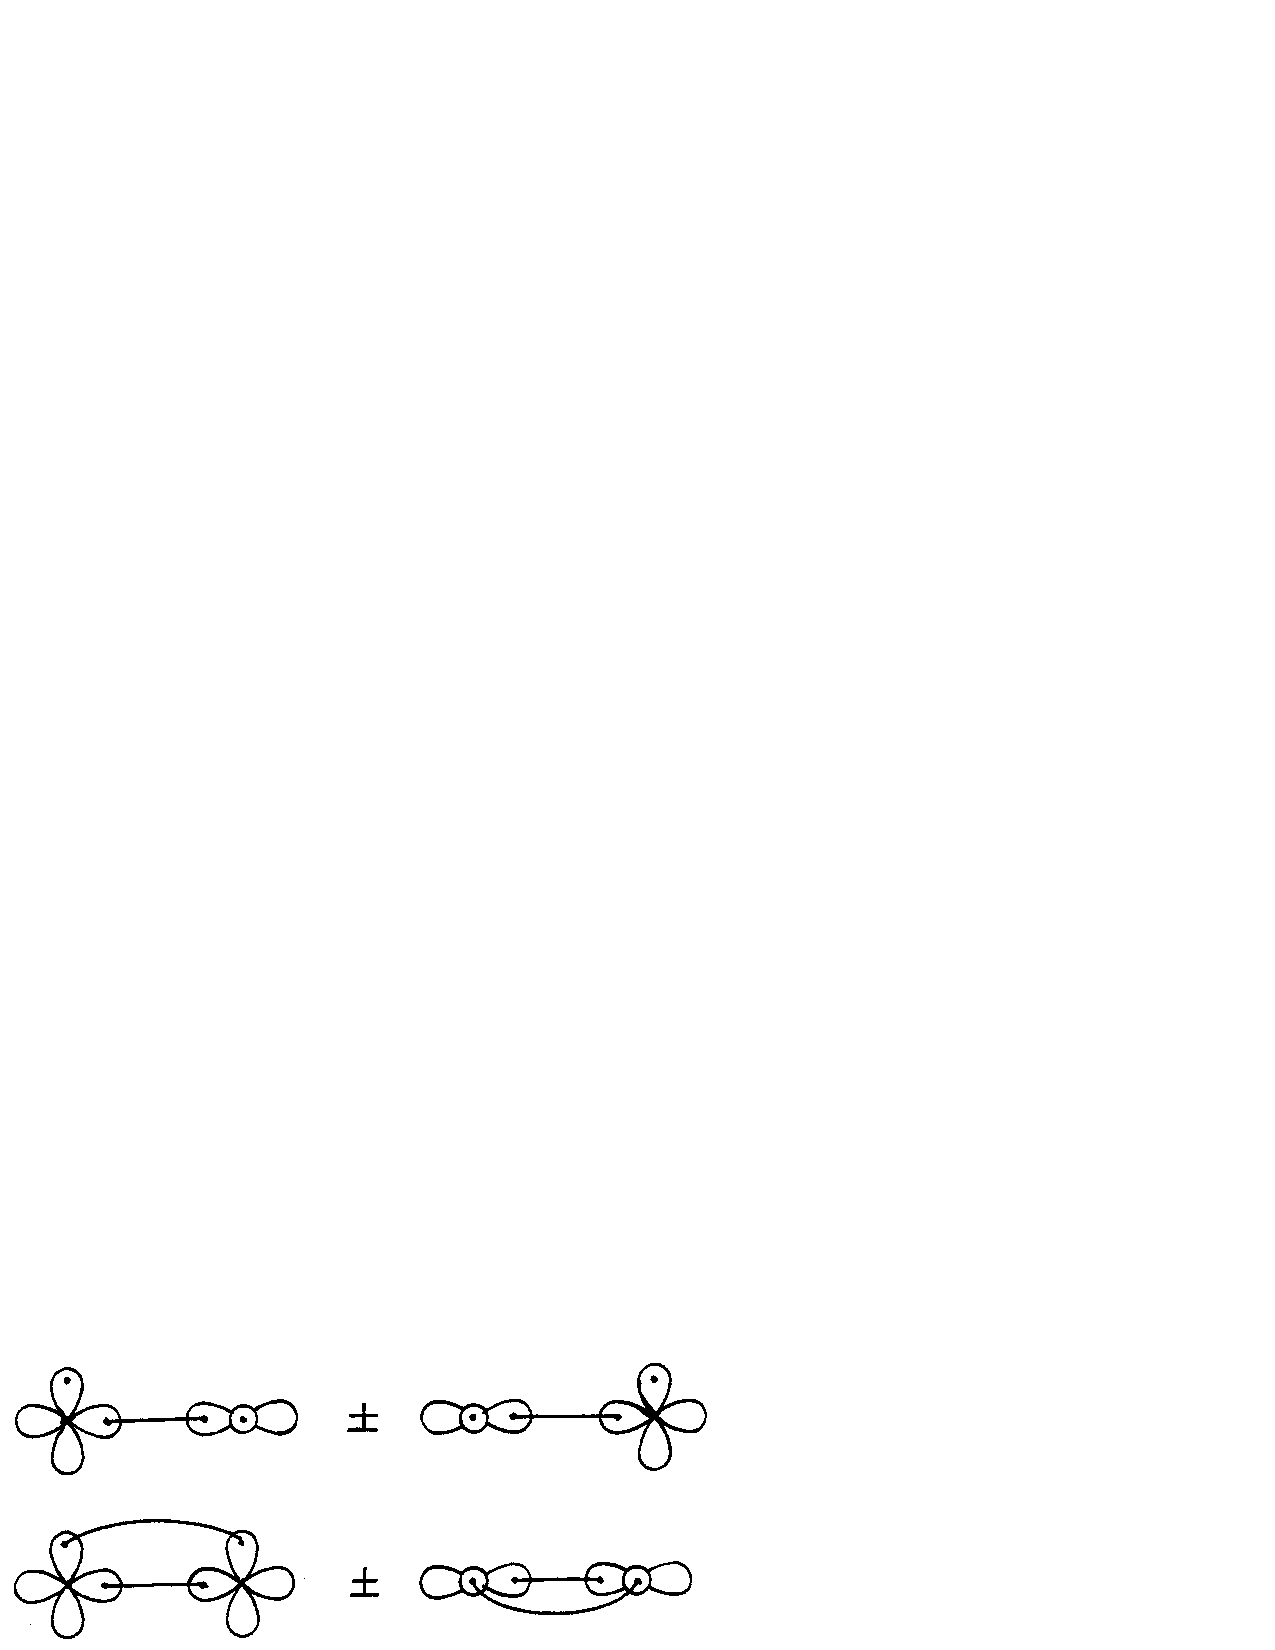
\includegraphics{fg10-5e}
\end{equation}
(the $3s$ pairs are not shown) corresponding to the MO configuration
\begin{equation}
\left( \sigma_g 3s \right)^2 \left( \sigma_u 3s \right)^2 \left( 
\sigma_g 3p \right)^2 \left( \pi_u 3p \right)^2
\label{chap10-eqno29}
\end{equation}
and leading to ${^3\Sigma}^-_g$ the lowest, ${^1\Delta}_g$, and 
${^1\Sigma}_g$.

However, since there is an empty $p$ orbital on each Si, we must also 
consider possible bonding of the $3s$ lobe orbitals as in Mg$_2$.
This leads to
\begin{equation}
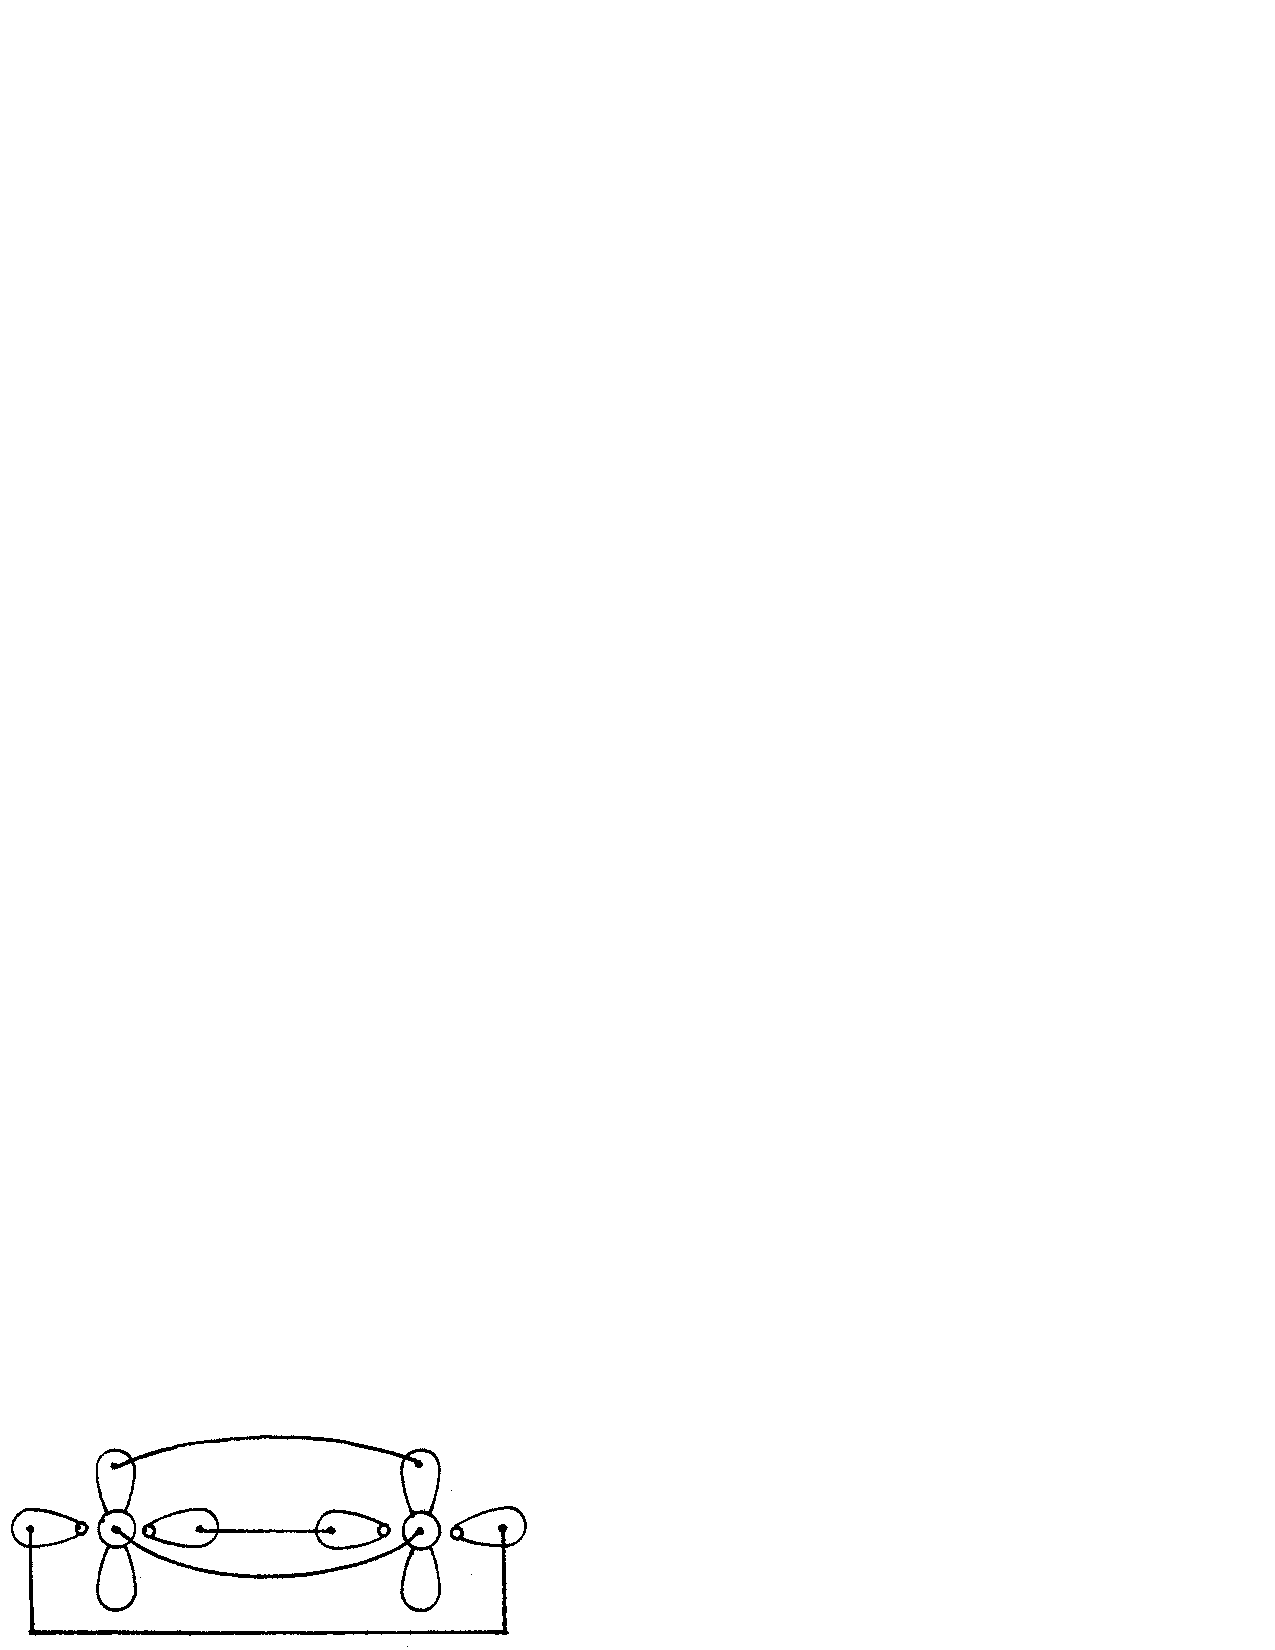
\includegraphics{fg10-5f}
\end{equation}
and hence, a ${^1\Sigma}^+_g$ state with MO configuration
\begin{equation}
\left( \sigma_g 3s \right)^2 \left( \sigma_u 3s \right)^2 \left( 
\pi_u 3p \right)^4.
\label{chap10-eqno30}
\end{equation}
Since the net $\sigma$ bond of Mg$_2$ is zero, the bonding in this
${^1\Sigma}^+_g$ state must be due to the two two-electron $\pi$
bonds.  A $\sigma$ bond leads to higher overlap and stronger bonding
than a $\pi$ bond, and hence, we expect, correctly, the
${^3\Sigma}^-_g$ state in equation (\ref{chap10-eqno29}) to be lower.

Another alternative to equation (\ref{chap10-eqno29}) arises from
bonding the lobe orbitals on one Si to the $p\sigma$ orbital of the
other Si, leading to
\begin{equation}
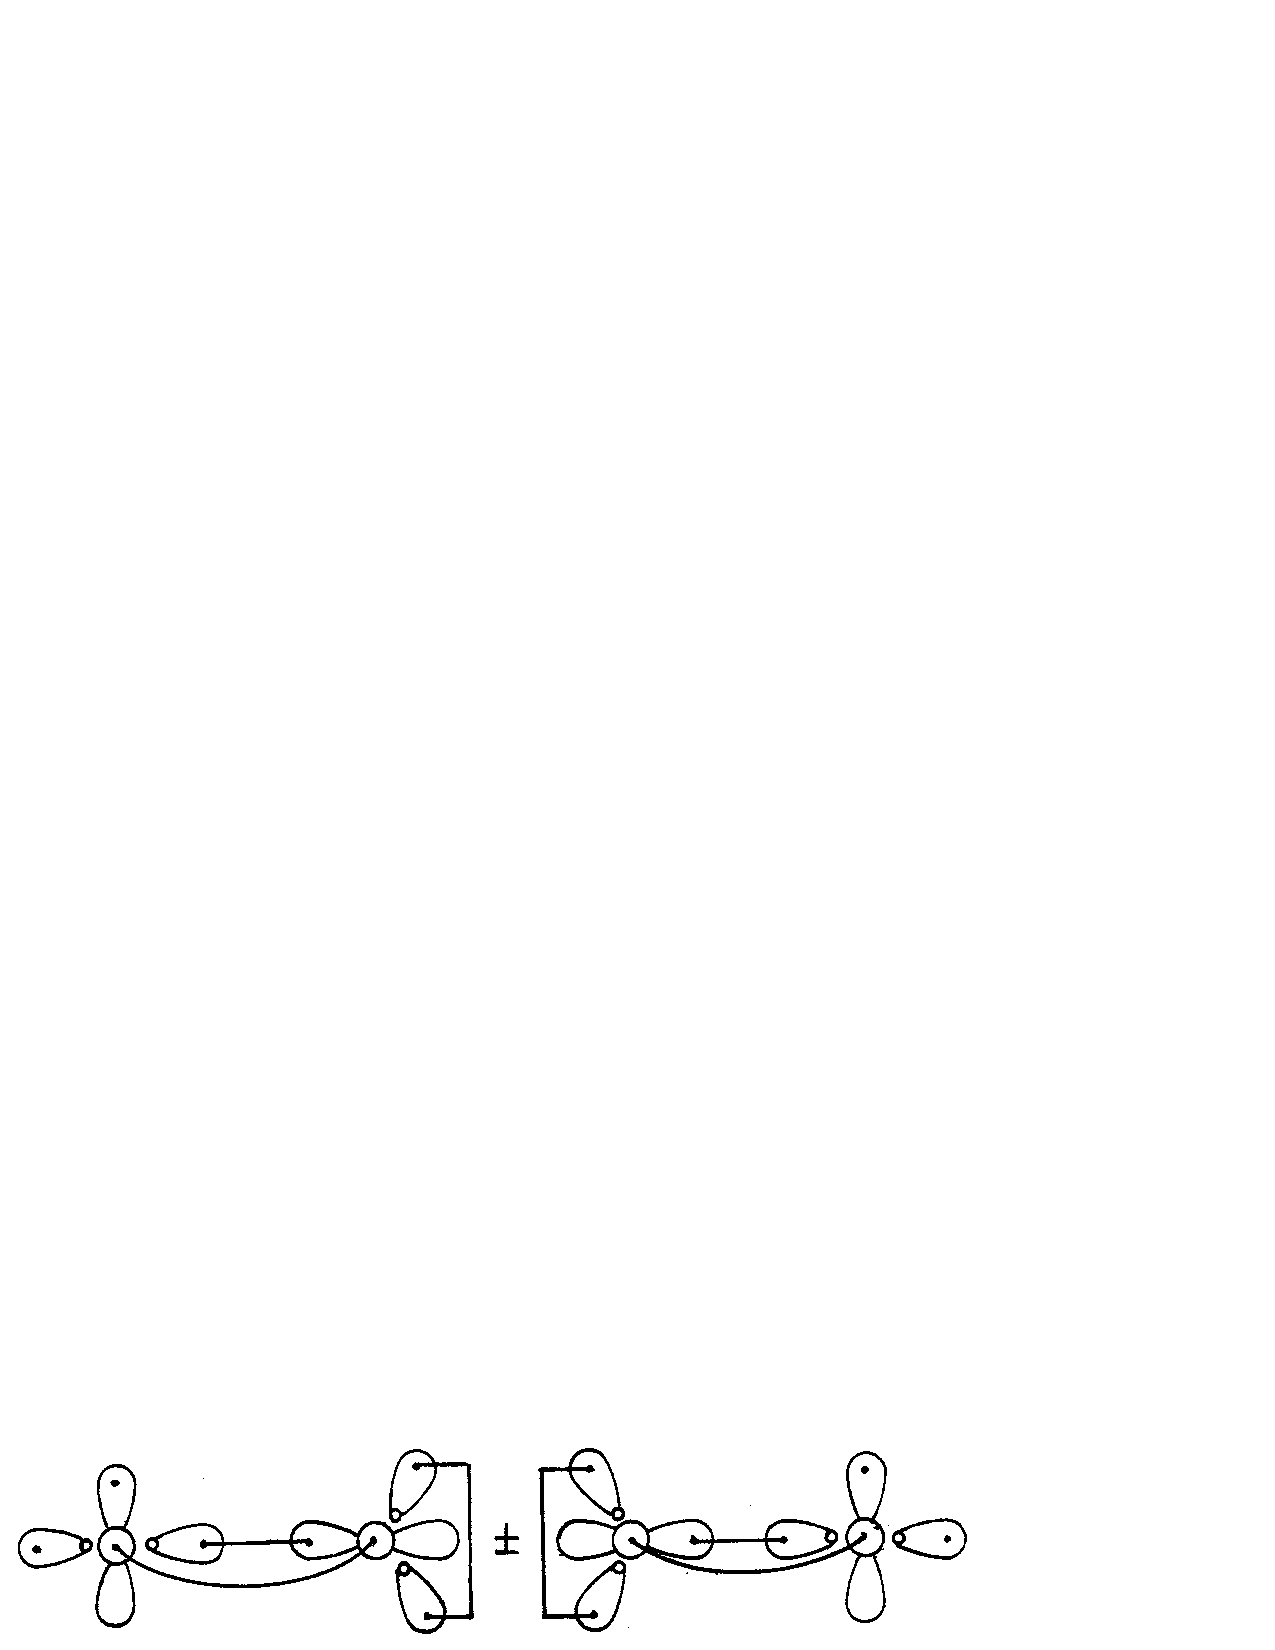
\includegraphics[scale=0.75]{fg10-5g}
\end{equation}
(now showing the lobe orbitals) with MO configuration
\begin{equation}
\left( \sigma_g 3s \right)^2 \left( \sigma_u 3s \right)^2 \left( 
\sigma_g 3p \right)^1 \left( \pi_u 3p \right)^3 .
\end{equation}
This leads to ${^3\Pi}_u$, the lowest, and ${^1\Pi}_u$ states.
However, this configuration being intermediate between equation
(\ref{chap10-eqno29}) and equation (\ref{chap10-eqno30}), is expected
to have an intermediate energy (it does).

\subsection{Al$_2$}

Just as for Si$_2$, we can form Al$_2$ in several ways.  First, with 
$p \sigma$ bonding
\begin{equation}
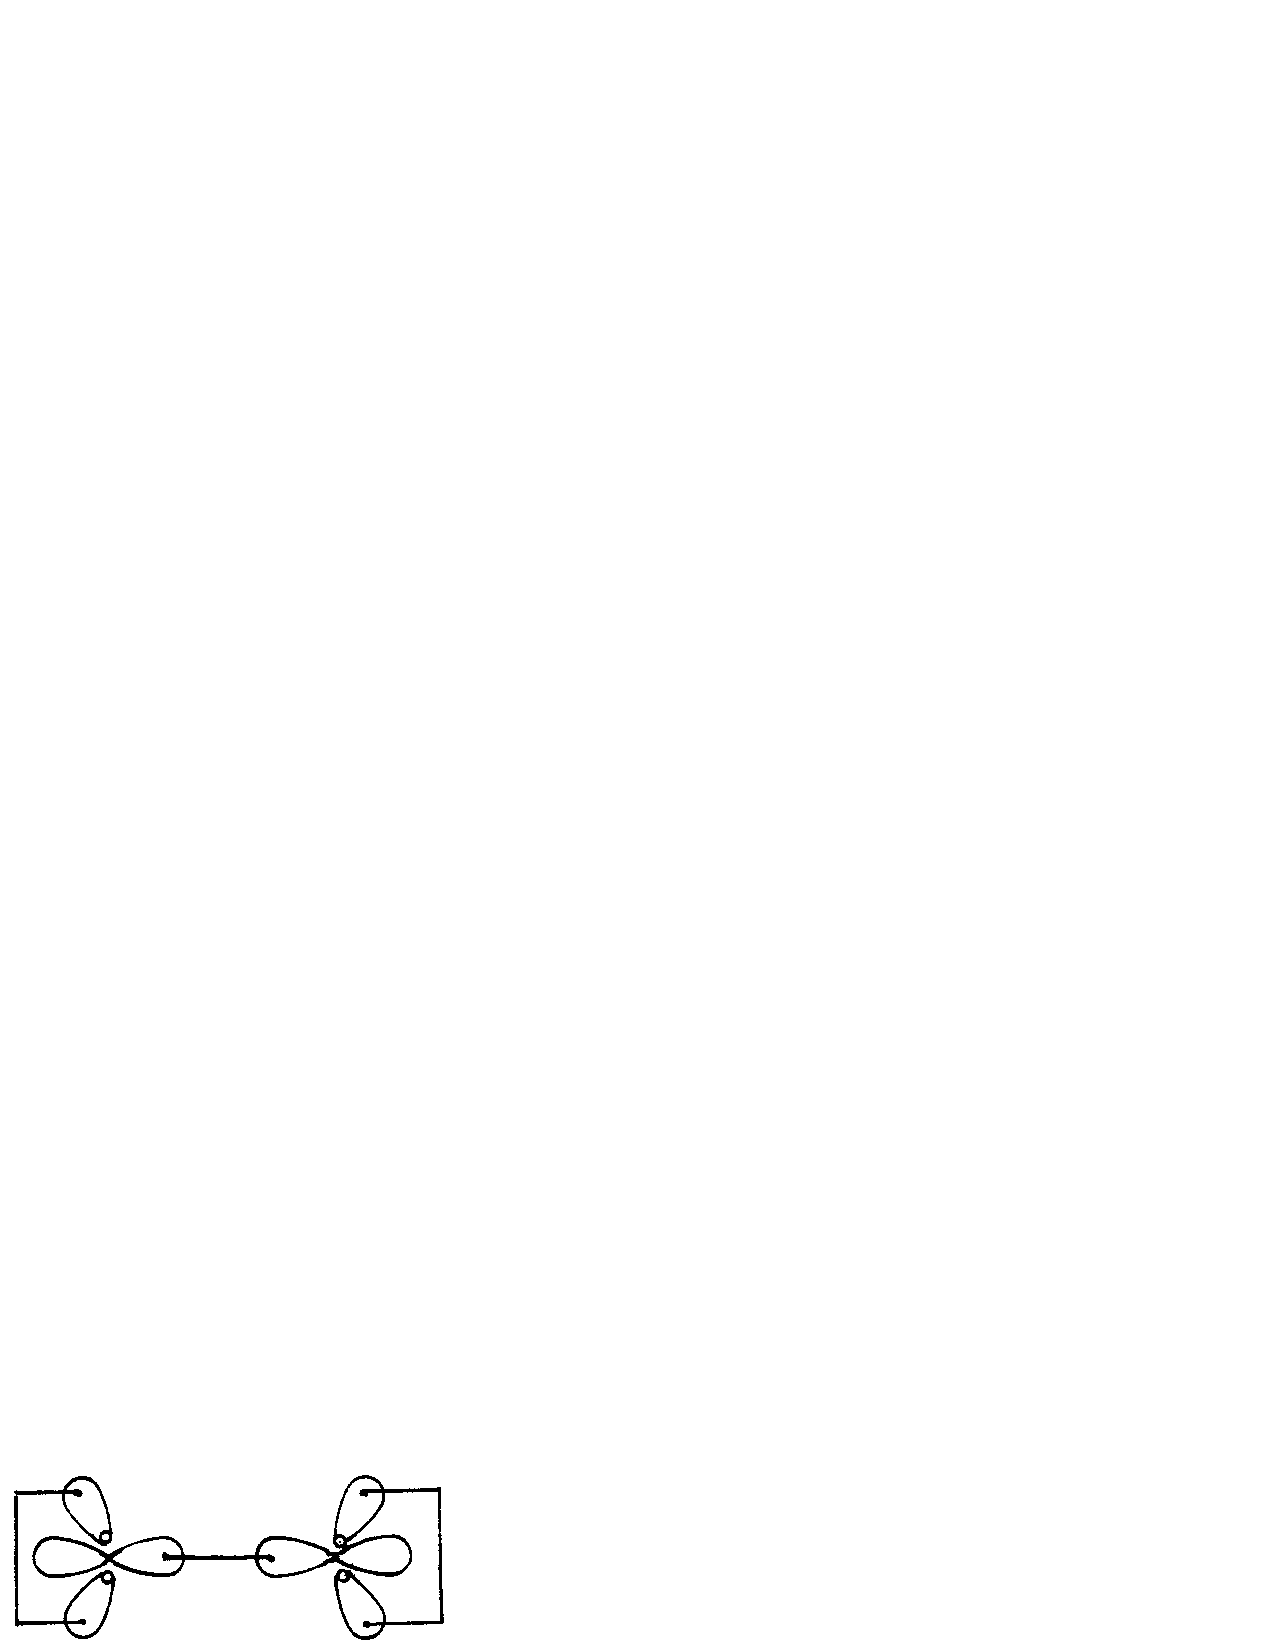
\includegraphics{fg10-5h}
\label{chap10-eqno31}
\end{equation}
leading to MO configuration
\begin{equation}
\left( \sigma_g 3s \right)^2 \left( \sigma_u 3s \right)^2 \left( 
\sigma_g 3p \right)^2
\end{equation}
and a ${^1\Sigma}^+_g$ state, or, second, with the lobe bonding
\begin{equation}
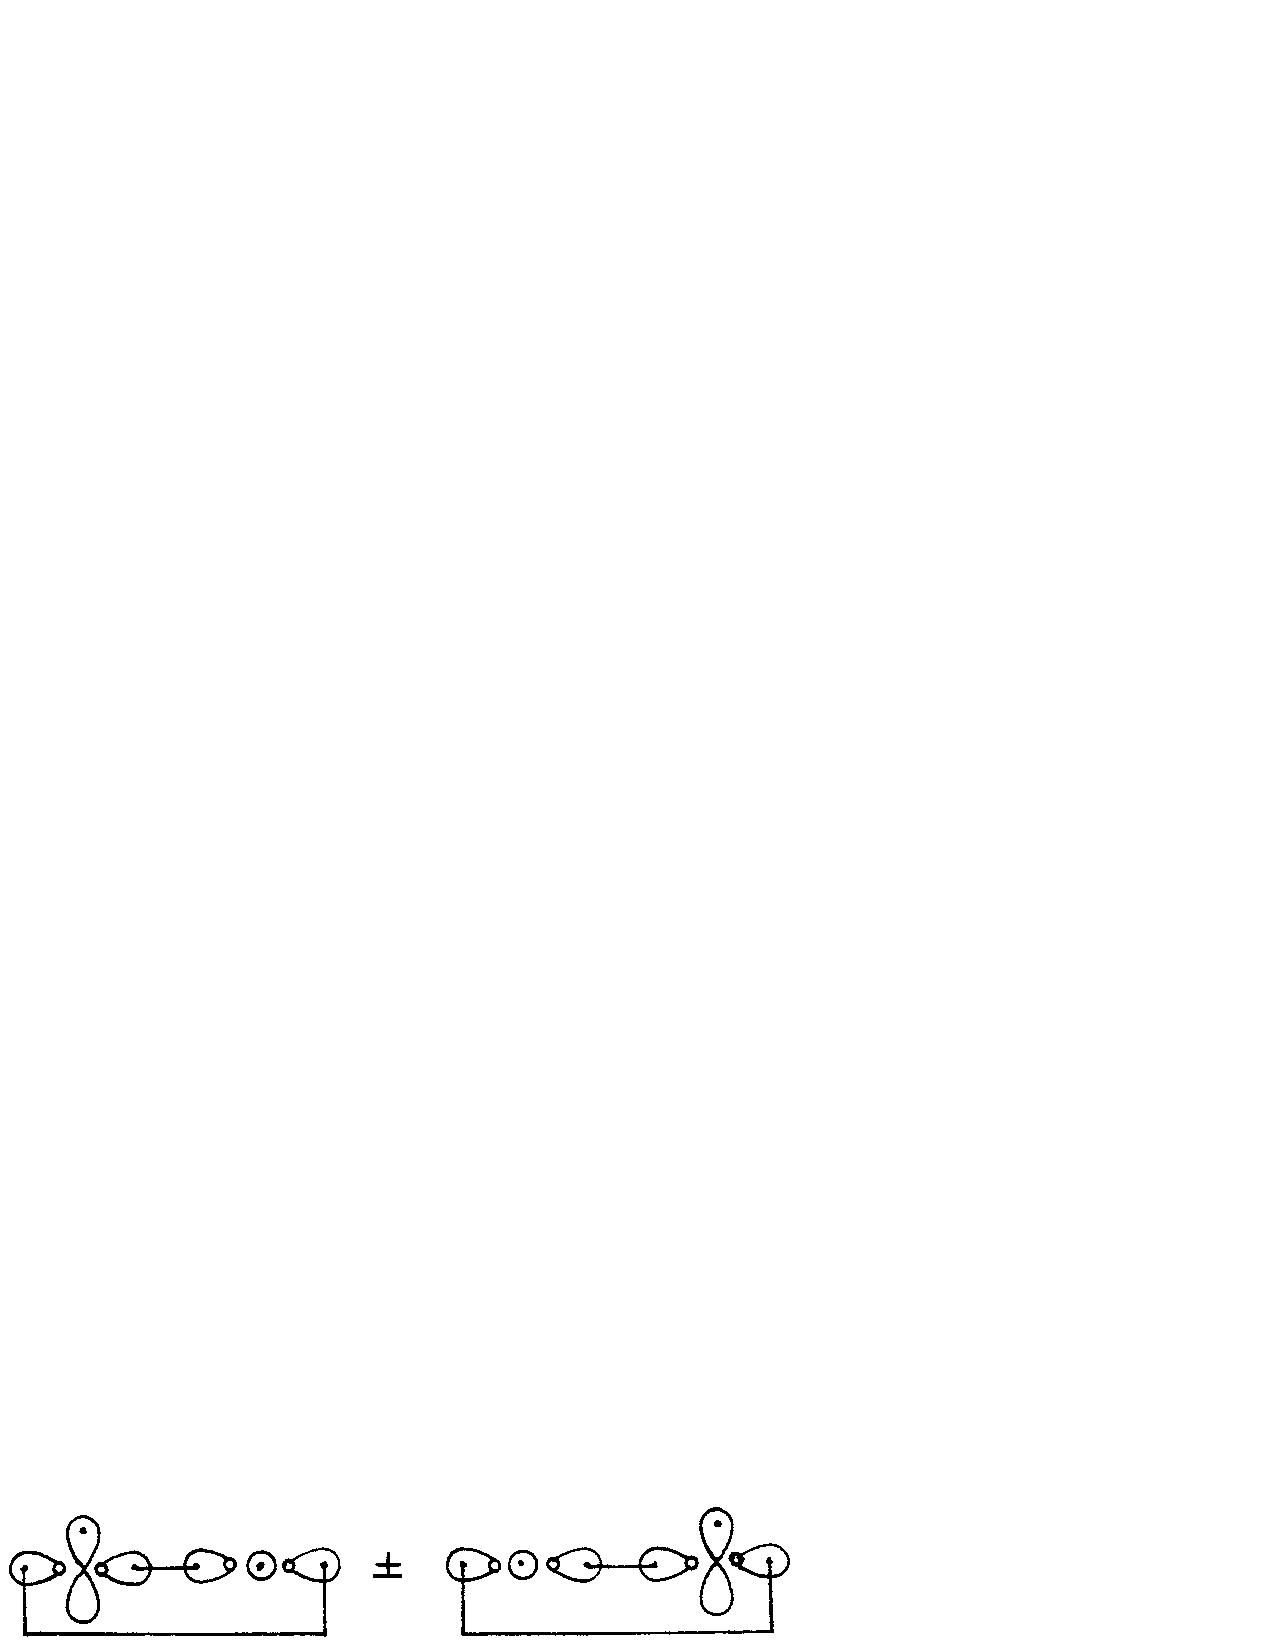
\includegraphics[scale=0.75]{fg10-5i}
\label{chap10-eqno32}
\end{equation}
leading to the MO configuration
\begin{equation}
\left( \sigma_g 3s \right)^2 \left( \sigma_u 3s \right)^2 \left( 
\pi_u 3p \right)^2 
\end{equation}
and a ${^3\Sigma}^-_g$ ground state.  Or, third,
the intermediate case with a bond between a $p$ orbital and a lobe orbital
\begin{equation}
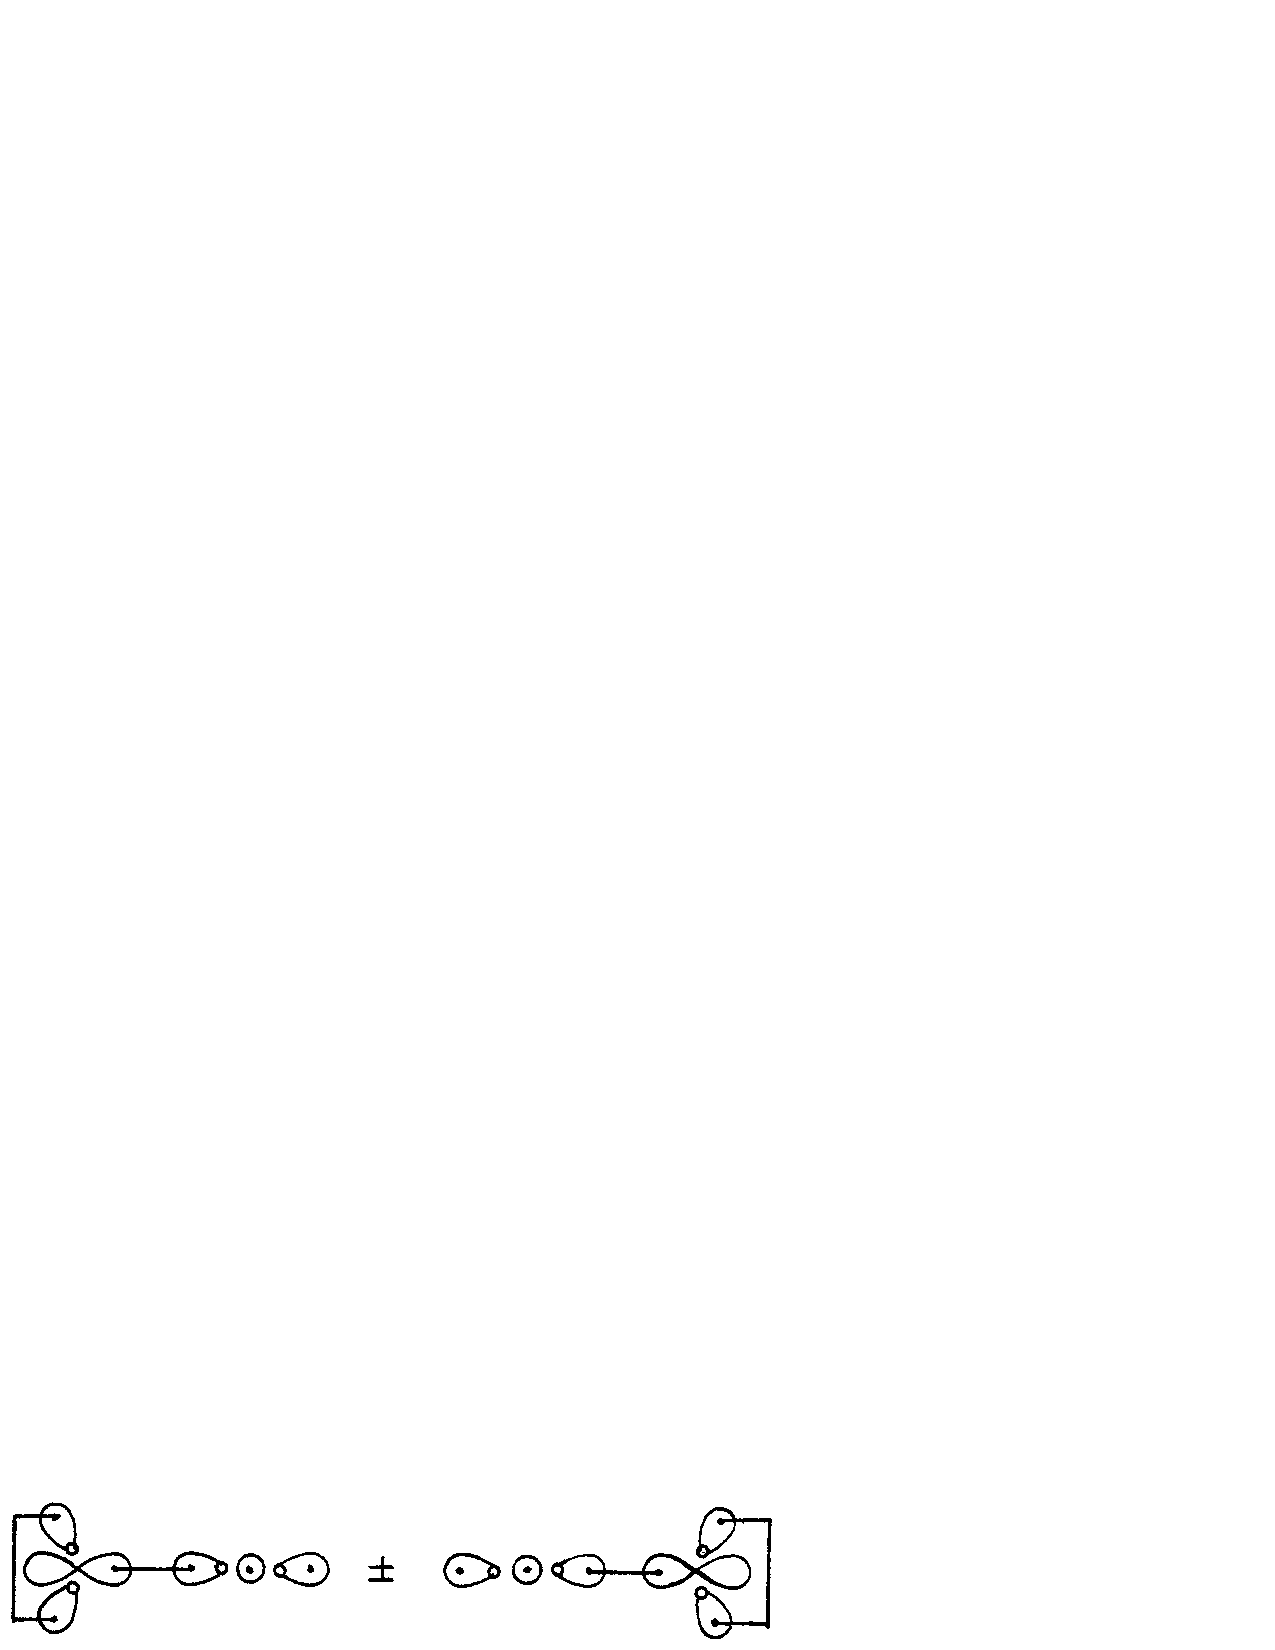
\includegraphics[scale=0.75]{fg10-5j}
\end{equation}
leading to MO configuration
\begin{equation}
\left( \sigma_g 3s \right)^2 \left( \sigma_u 3s \right)^2 \left( 
\sigma_g 3p \right)^1 \left( \pi_u 3p \right)^1
\end{equation}
and a ${^3\Pi}_u$ ground state.

The comparison between equation (\ref{chap10-eqno31}) and equation
(\ref{chap10-eqno32}) is that of a two-electron $\sigma$ bond versus
two one-electron $\pi$ bonds. As shown in Figure
\ref{chap10-fig6}, 
the one-electron $\pi$ bonds are each better than  half as good as a 
two-electron $\sigma$ bond,
leading to a ${^3\Sigma}^-_g$ ground state.

\begin{figure}
\begin{center}
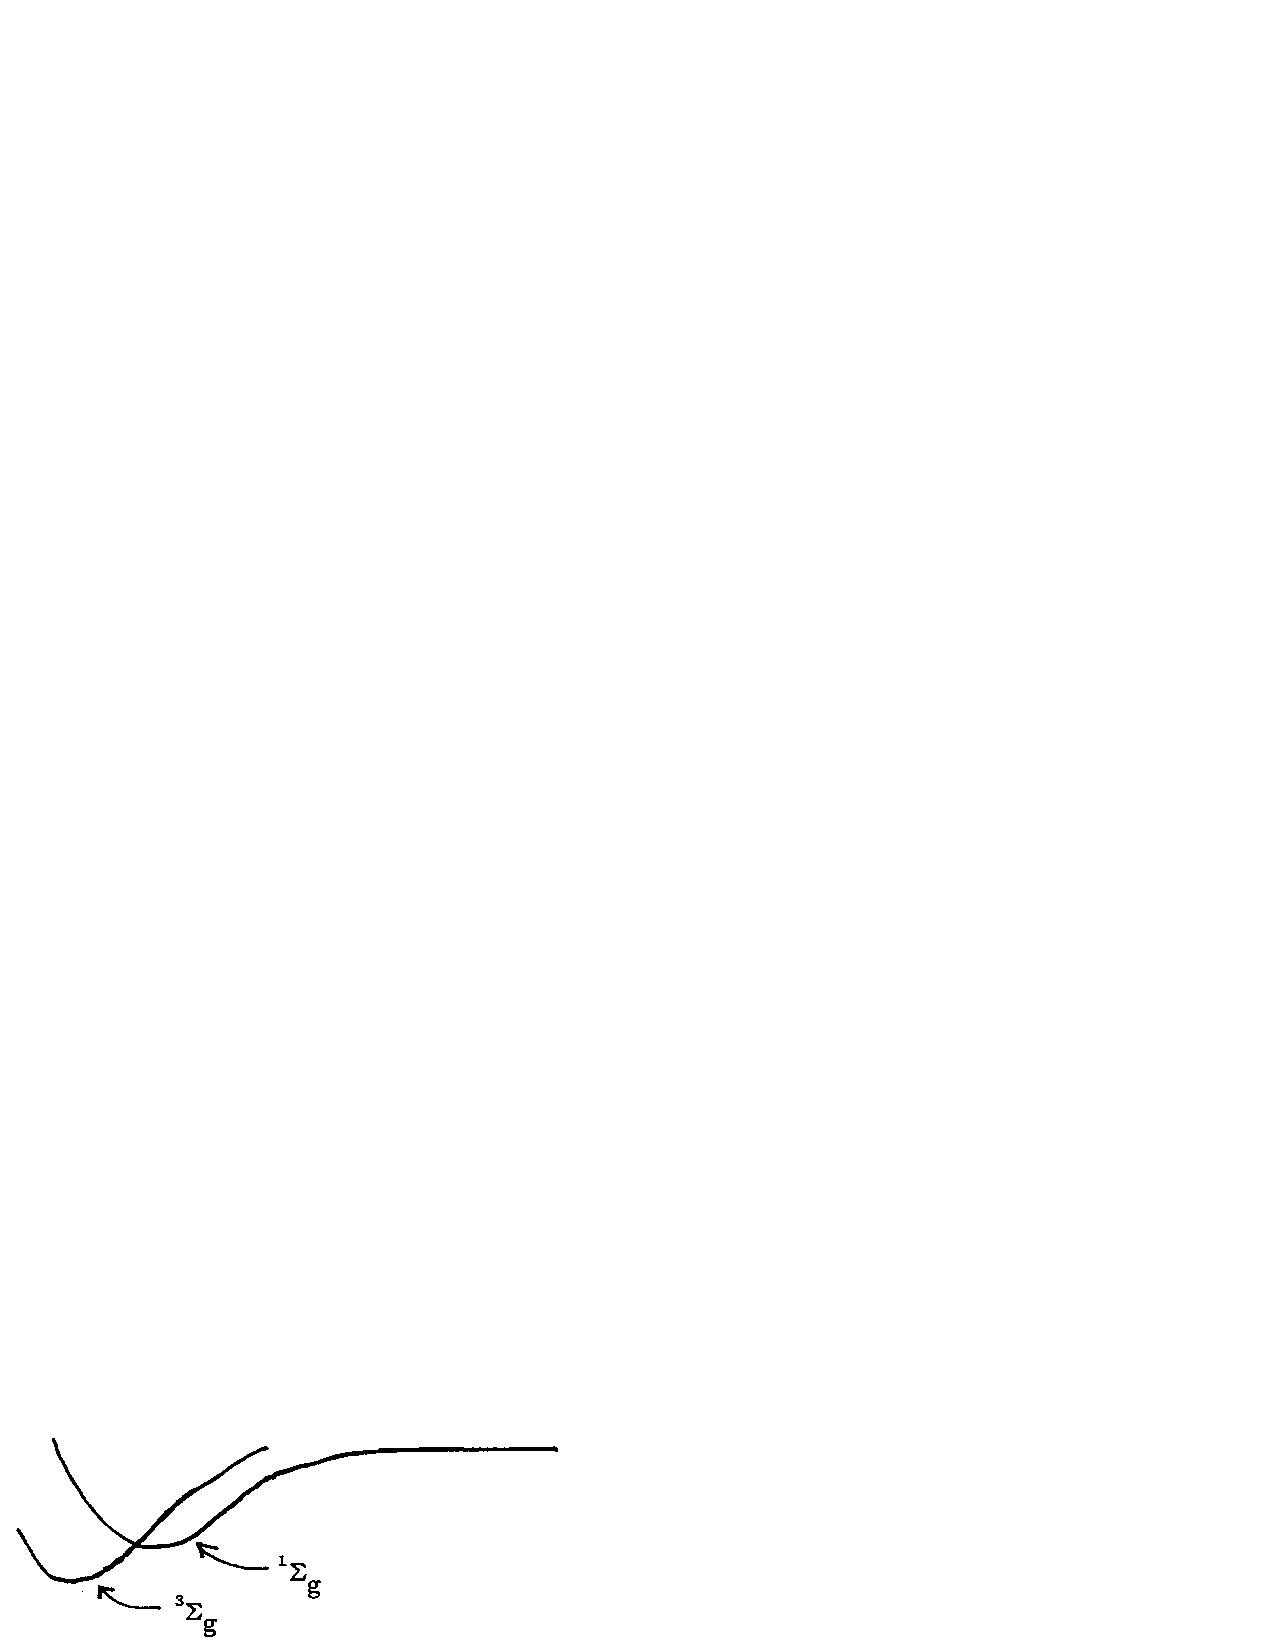
\includegraphics[scale=0.75]{fg10-6}
\end{center}
\caption{The potential curve for Al$_2$.}
\label{chap10-fig6}
\end{figure}

\subsection{The Molecular Orbitals}

\begin{figure}
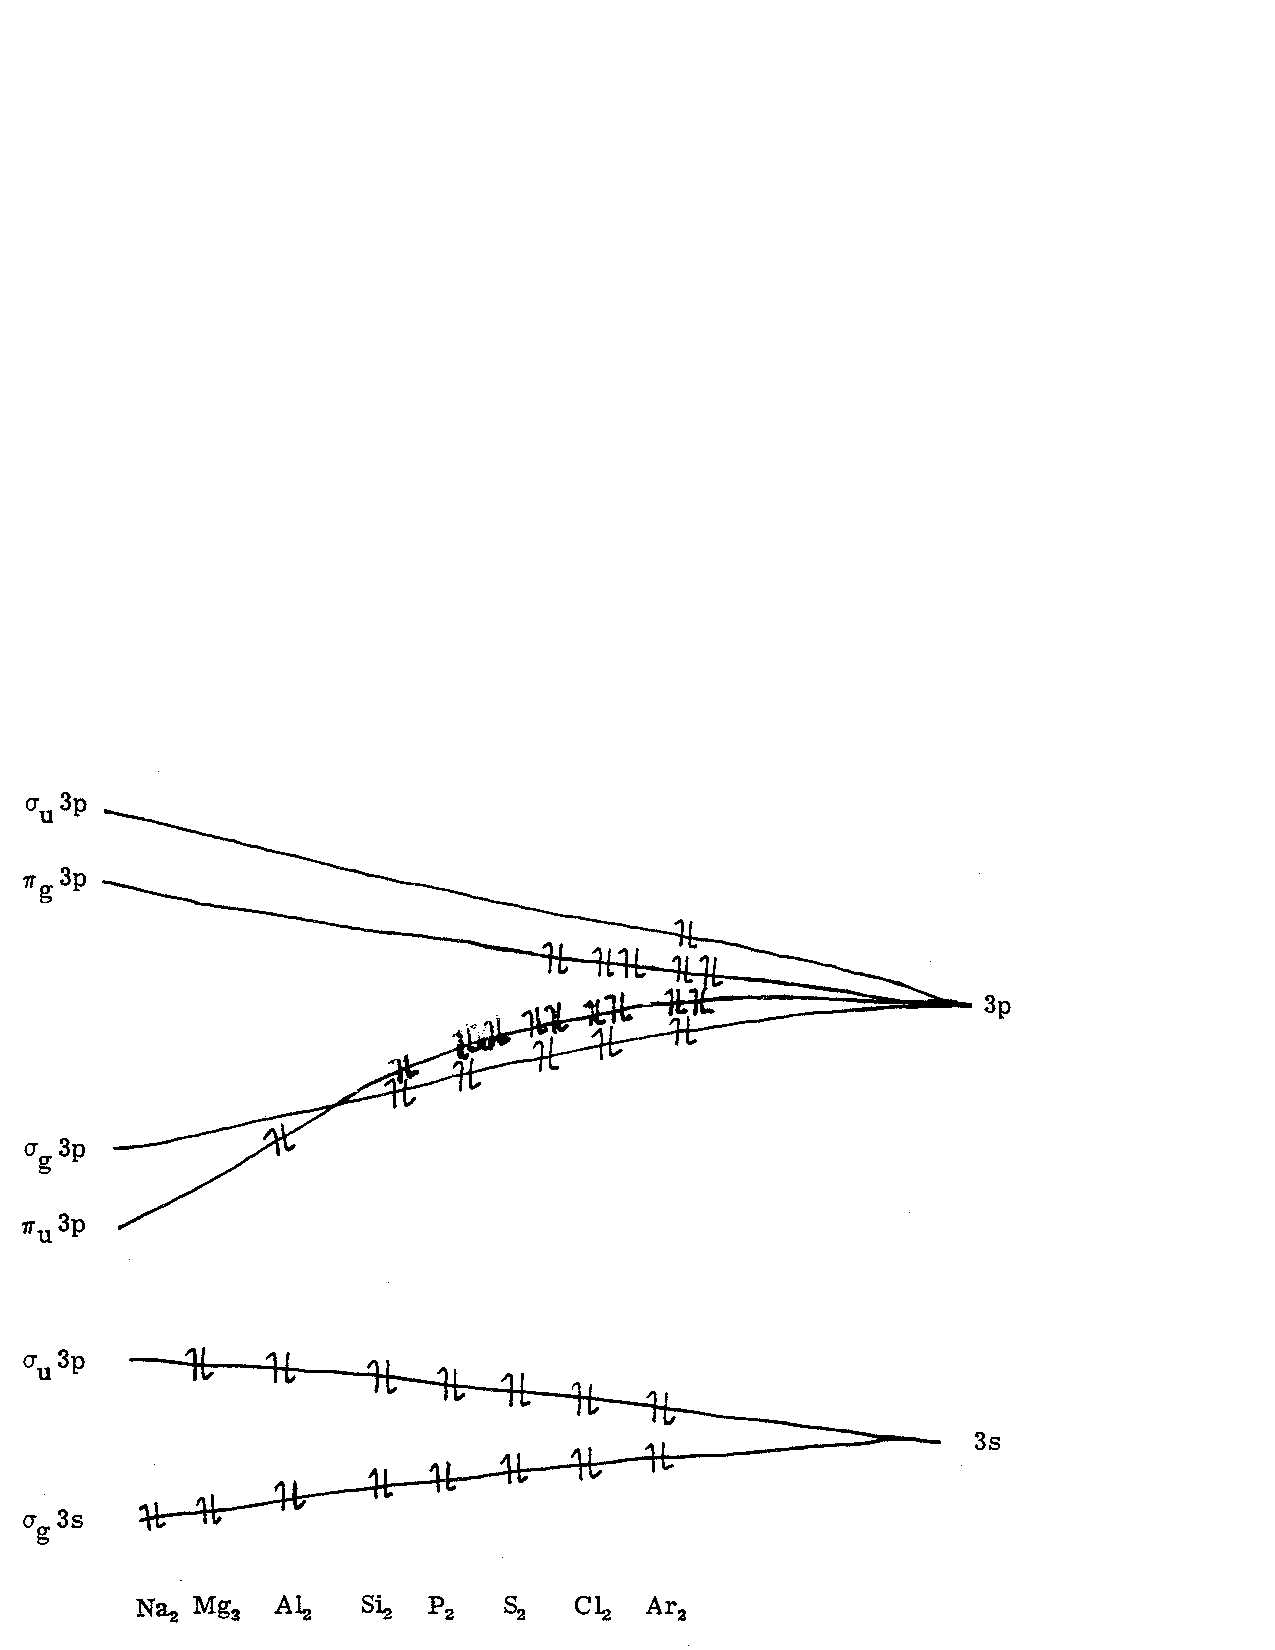
\includegraphics[scale=0.75]{fg10-7}
\caption{The MO correlation for second row diatomics.}
\label{chap10-fig7}
\end{figure}

The ground state configurations and bonding, discussed above, can be 
rationalized in terms of the following MO 
scheme.  Assuming that the ordering of the MOs 
varies monotonically as we proceed from Na$_2$ to Ar$_2$, as in Figure 
\ref{chap10-fig7}, then the predicted configurations obtained by
filling the lowest orbitals with electrons leads to agreement with
experiment.  In deriving this diagram, we made use of the orbital
ordering for $R = \infty$, plus the orderings, from the nodal theorem,
\begin{equation}
\sigma_g 3s < \sigma_u 3s ,
\end{equation}
\begin{equation}
\sigma_g 3p < \sigma_u 3p ,
\end{equation}
and
\begin{equation}
\pi_u 3p < \pi_g 3p ,
\end{equation}
plus the \emph{ad hoc} assumption that
\begin{equation}
\sigma_g 3p < \pi_u 3p
\end{equation}
for	Si, P, S, Cl, and Ar, while
\begin{equation}
\sigma_g 3p > \pi_u 3p
\end{equation}
for Al (and presumably Na and Mg).  Later, in this chapter, we
consider a more detailed analysis of correlation diagrams.

This section used the second, Si, row as the prototype homonuclear 
diatomics.  In the following sections, we will examine diatomics for 
other rows.  An overall trend is that atoms with more core electrons 
have larger bond distances, smaller overlaps, and weaker bonds.  In 
addition, we find that first row atoms, the C row, can make very 
strong $\pi$ bonds leading, in some cases, to different ground states 
from these described above.


\section{Columns}

\subsection{The Li Column}

\subsubsection{Alkali Diatomics}

The properties of homonuclear diatomics with one or two valence
electrons are listed in Table \ref{chap10-tab8}.  Proceeding from
Li$_2$ to Cs$_2$, we find a gradual increase in bond length, 2.67 to
4.47 \AA, and a gradual decrease in bond energy, 1.05 to 0.39 eV.
	
\begin{table}
\caption{ Properties of alkali diatomic molecules.$^a$}
\label{chap10-tab8}
\begin{tabular}{ccccccc}\\ \hline

& $R_e$ & $\omega_e$ &\multicolumn{2}{c}{$D_0$} &
\multicolumn{2}{c}{IP (eV)}\cr
& (\AA) &  (cm$^{-1}$)& (eV) & (kcal) & molecule & atom$^b$\cr
H$_2^+$ & 1.052	 & 2321.$^7$ & 2.6508 & 61.13\cr
H$_2$ & 0.7414 & 4401.2 & 4.4781 & 103.26 & 15.4259 & 13.595\cr
Li$^+_2$ & - & - & 1.4$^4$ & 33.2 & - & - \cr
Li$_2$ & 2.6729 & 351.4 & 1.04$^6$ & 24.12 & 5.0$^0$ & 5.39\cr
Na$^+_2$ & (3.54) & (126) & 0.96 & 22.1 & - & -\cr
Na$_2$ & 3.0789 & 159.1 & 0.720	 & 16.60 & 4.90 & 5.138\cr
K$^+_2$ & (4.11) & (67) & 0.87$^5$ & 19.6\cr
K$_2$ & 3.9051 & 92.0 & 0.514 & 11.85 & 4.0 & 4.339\cr
Rb$^+_2$ & (3.94) & - & $\geq$0. 72 & $\geq$16.6\cr
Rb$_2$ & - & 57.3 & 0.49 & 11.3 & 3.$^7$ & 4.176\cr
Cs$^+_2$ & - & - & 0.61 & 14.1\cr
Cs$_2$ & 4.47 & 42.0 & 0.394 & 9.09 & 3.$^7$ & 3.893\cr
LiNa & 2.81	& 256.8 & 0.90 & 20.8 & 4.94 & 5.138\cr
LiK & & & 0.81 & 18.7 & 4.69 & 4.339\cr
LiRb\cr
LiCs\cr
NaK & 3.58$^9$ & 124.1 & 0.63 & 14.5 & 4.57 & 4.339\cr
NaRb & & 106.6\cr
NaCs\cr
KRb\cr
KCs\cr
RbCs & & 49.4\cr
\hline
\end{tabular}\\
$^a$See reference 1.
$^b$Table 5-4 of Chapter 5.
\end{table}

In the last section, we mentioned that the one-electron bond in 
Na$_2^+$ is stronger than the two-electron bond
\begin{equation}
D_0 \left( {\rm Na}^+_2 \right) = 0.96 ~ {\rm eV} = 22.1 ~ {\rm kcal}
\end{equation}
and
\begin{equation}
D_0 \left( {\rm Na}_2 \right) = 0.72 ~ {\rm eV} = 16.6 ~ {\rm kcal},
\end{equation}
whereas, for H$^+_2$ and H$_2$, the opposite result is found
\begin{equation}
D_0 \left( {\rm H}^+_2 \right) = 2.65 ~ {\rm eV} = 61.1 ~ {\rm kcal}
\end{equation}
and
\begin{equation}
D_0 \left( {\rm H}_2 \right) = 4.48~{\rm eV} = 103.3 {\rm kcal}
\end{equation}
One can understand these dramatic differences, as follows.  From 
Chapter 2 the one-electron bond is of the form
\begin{equation}
D_{one} = {| \tau | \over 1 + S} ,
\end{equation}
where $S$ is the overlap, and
\begin{equation}
\tau = \langle l | h | r \rangle - S \langle l | h | l \rangle
\end{equation}
is large and negative.  While the 
one-electron part of the two-electron bond is
\begin{equation}
D_{two} \cong {2S|\tau| \over 1 + S^2} .
\end{equation}
At the energy minimum for H$_2$, the overlap is $S \approx 0.7$, so that
\begin{equation}
D_{one} = 0. 59 | \tau |
\end{equation}
and
\begin{equation}
D_{two} =  0.94 | \tau | .
\end{equation}
This suggests that
\begin{equation}
{D_{two} \over D_{one}} = 1.6
\end{equation}
is in good agreement with the experimental value of 1.7.

Now consider Na$_2$. Two effects conspire to yield a small overlap. 
First, the Na $3s$ orbital is much larger than the H $1s$ orbital, and 
hence, the region of maximal $| \tau |$ is at larger $R$, leading to a 
smaller $S$.  Second, as the atoms are brought together, the $3s$ 
orbital on the left must get orthogonal to the Na core of the 
right atom, Pauli principle, and similarly, for the $3s$ orbital
on the right.  This increases the bond distance and weakens the bond. The 
optimum bond length occurs at a point where the $3s_l - 3s_r$ 
overlap is large, but the core-valence overlap still small.  The 
optimum overlap is $S \sim 0. 3$, which, would imply
\begin{equation}
{D_{two} \over D_{one}} = 0. 71 , 
\end{equation}
approximately the observed value.  The difference between the one-electron 
bond and the two-electron bond is
\begin{equation}
\Delta D = D_0 \left( M^+_2 \right) - D_0 (M_2)
\end{equation}
seems to fluctuate with values of
0.39, 0.24, 0.34, 0. 23, 0.22 for Li through Cs.
This may be due to the inaccuracy in current values for these quantities.

Since it is obviously hard to study the properties of positive ions, such
as Na$^+_2$, one wonder how the $D_0(M^+_2)$ are determined.  Current values 
were obtained indirectly as
\begin{equation}
D_{one} = D_{two} + \mathrm{IP}(Na) - \mathrm{IP}(Na_2),
\end{equation}
using the cycle indicated in Figure \ref{chap10-fig8}.

\begin{figure}
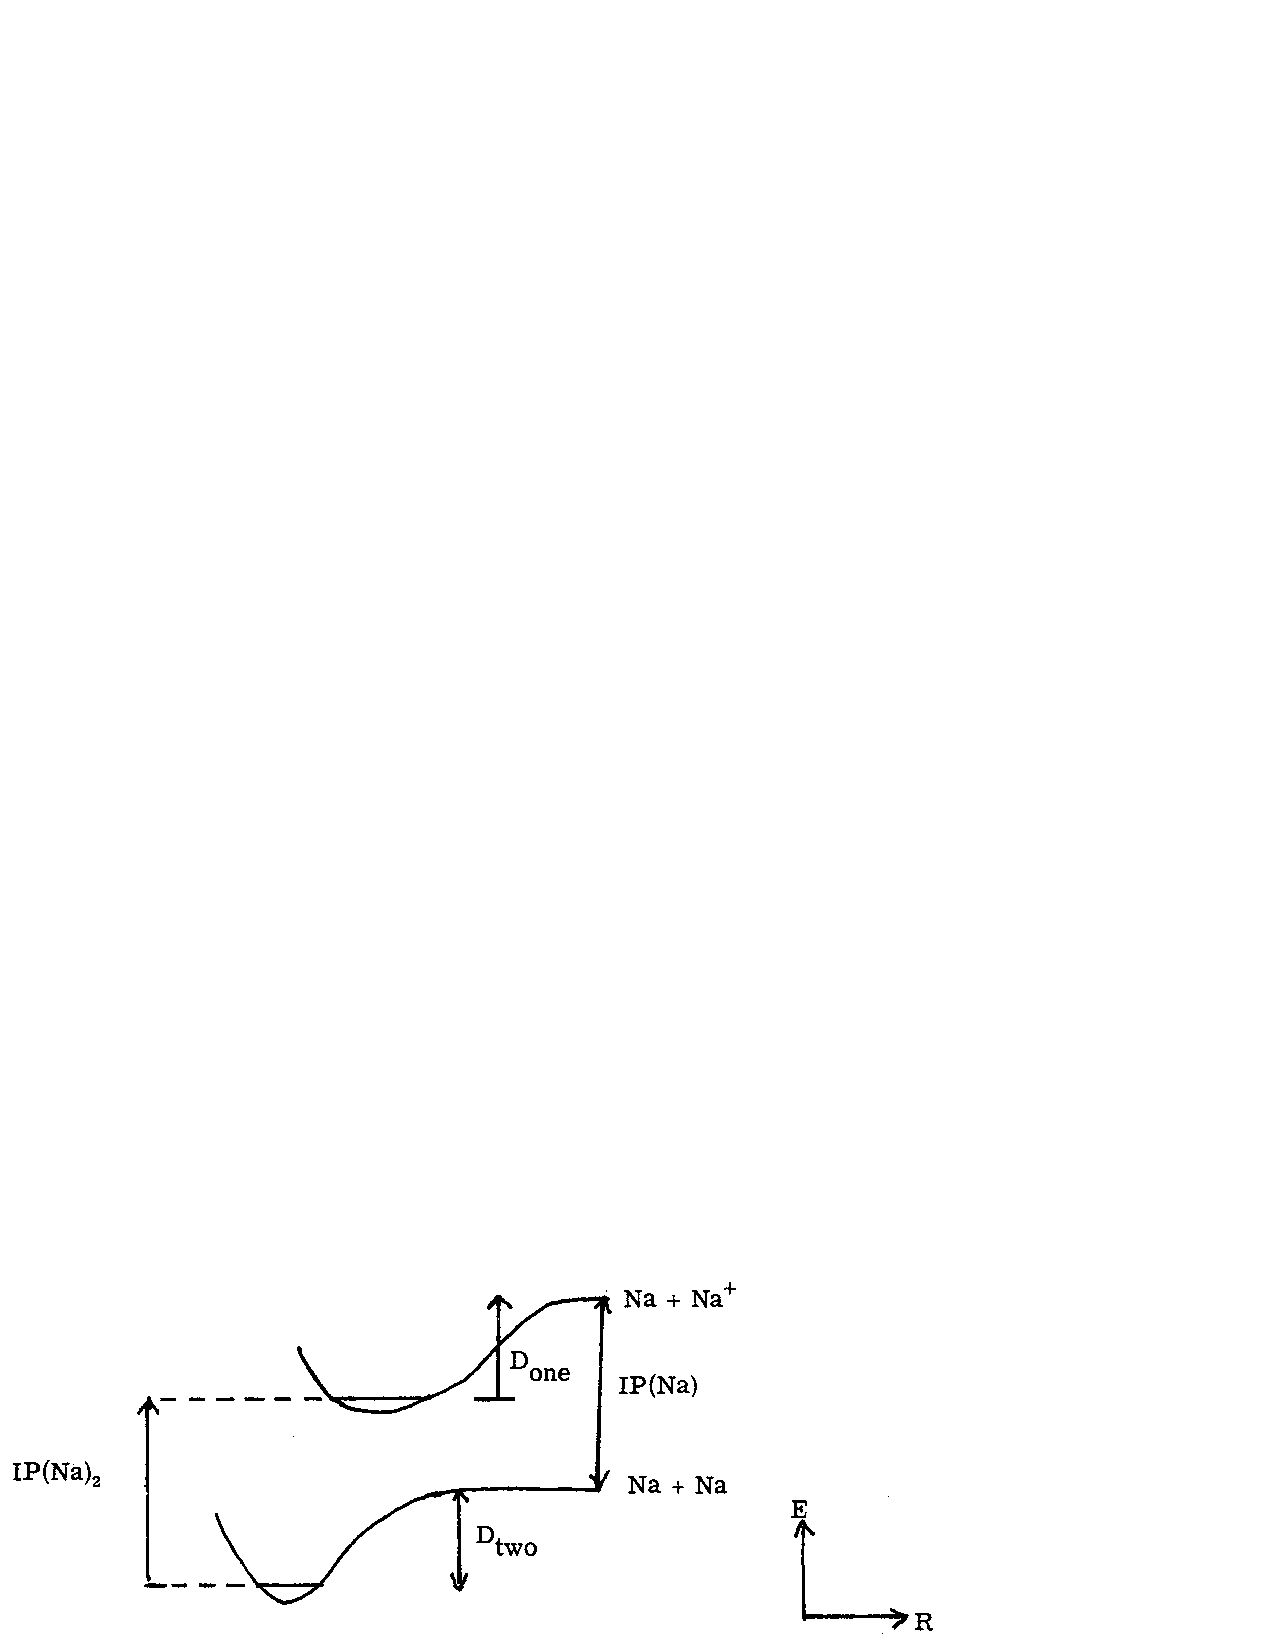
\includegraphics[scale=0.75]{fg10-8}
\caption{}
\label{chap10-fig8}
\end{figure}

Thus, by measuring the ionization potential of N$_2$ and
Na and the bond energy of Na$_2$, we obtain the bond energy of 
Na$^+_2$.  Since $\mathrm{IP}(\mathrm{Na}_2) < \mathrm{IP}(\mathrm{Na})$, 
then $D_{one} > D_{two}$.

\subsubsection{The Cu$_2$ Sequence}

The noble metal Cu has the valence configuration $(3d)^{10} (4s)^1$.
Since the $3d$ orbitals are small compared to the $4s$ orbital, the
neutral atom is analogous to K, with a $(4s)^1$ configuration. The
difference between Cu and K is that the $4s$ orbital of Cu is smaller
(see Figures \ref{fig5-10a}--\ref{fig5-10g}) and considerably more
strongly bound, $\mathrm{IP}_{\mathrm{Cu}} = 7.72$ eV and
$\mathrm{IP}_\mathrm{K} = 4.339$ eV.  This is because the $4s$ orbital
of Cu penetrates inside the $3d$ orbital, allowing it to see a
considerably higher effective nuclear charge.  The result is shorter,
stronger bonds for the noble metals, see Tables
\ref{chap10-tab9}--\ref{chap10-tab10}.

\begin{table}
\caption{Properties of noble metal diatomics.$^a$}
\label{chap10-tab9}
\begin{tabular}{ccccccc}\\ \hline

& $R_e$ & $\omega_e$ &\multicolumn{2}{c}{$D_0$}&
\multicolumn{2}{c}{IP (eV)}\cr
& (\AA)&(cm$^{-1}$) &(eV) &(kcal) & Molecule & Atom$^b$\cr
Cu$_2$ & 2.2197 & [264.6] & 2.03 & 46.8 & 7.3$^7$ & 7. 724$^b$\cr
Ag$_2$ & & 192.4 & 1.66 & 38.3 & & 7.574\cr
Au$_2$ & 2.4719 & 190.9 & 2.30 & 53.0 & & 9.22\cr
CuAg & & 231.8 & 1.7$^6$ & 40.6\cr
CuAu & & 25 & 2.3$^6$ & 54.4\cr
AgAu & & 200 & 2.0$^6$ & 47.5\cr
CuLi & & & 1.98 & 45.7\cr
CuNa & & & 1.7$^9$ & 41.3\cr
AgLi & & & 1.81 & 41.7\cr
AgNa & & & 1.40 & 32.3\cr
AuLi & & & 2.92 & 67.3\cr
\hline
\end{tabular}\\
$^a$See reference 1.
$^b$Table 5-4 of Chapter 5.
\end{table}

\begin{table}
\caption{}
\label{chap10-tab10}
\begin{tabular}{ccccc}\\ \hline
& $R_e$ (\AA)& $\omega_e$ (cm$^{-1}$)& $D_0$ (kcal) & IP (eV)\cr
K$_2$ & 3.39 & 92 & 11.9 & 4.0\cr
Cu$_2$ & 2.20 & 265 & 46.8 & 7.4\cr
\hline
\end{tabular}
\end{table}



\subsubsection{The Heteronuclear Sequence}

\begin{table}
\caption{Heteronuclear bonding for alkali and noble metals.$^a$}
\label{chap10-tab11}
\begin{tabular}{ccccccc}\\ \hline
&\multicolumn{2}{c}{$R_e$ (\AA)}&\multicolumn{2}{c}{$D_0$ (kcal)}
&&$\Delta D$ (kcal)\cr
&$XY$ & ${1\over 2}(X_2+Y_2)$ & $XY$ & ${1\over 2}(X_2+Y_2)$ &
$\sqrt{X_2\times Y_2}$\cr
LiNa & 2.81	 & 2.876 & 20.8 & 20.4 & 20.0 & 0.8\cr
LiK	& & & 18.7 & 18.0 & 16.9 & 1.8\cr
NaK & 3.59 & 3.49 & 14.5 & 14.2 & 14.0 & 0.5\cr
CuAg & & & 40.6 & 42.6 & 42.3 & $-$1.7\cr
CuAu & & & 54.4 & 49.9 & 49.8 & 4.6\cr
AgAu & & & 47.5 & 40.7 & 45.1 & 2.4\cr
CuLi & & & 45.7 & 35.5 & 33.6 & 12.1\cr
CuNa & & & 41.3 & 31.7 & 27.9 & 13.4\cr
AgLi & & & 41.7 & 31.2 & 30.4 & 10.7\cr
AgNa & & & 32.3 & 27.5 & 25.2 & 7.1\cr
AuLi & & & 67.3 & 38.6 & 35.7 & 31.6\cr
\hline
\end{tabular}
\end{table}

Experimental results are often not available for the heteronuclear
molecules XY, and it would be useful to have a reliable means for
predicting the properties of XY in terms of averages for molecules
X$_2$ and Y$_2$. Some results are given in Table \ref{chap10-tab11}.
It is speculated that a heteronuclear bond xy, with no charge
transfer, would be equal to the geometric mean of the homonuclear bond
energies,
\begin{equation}
D_{xy} = \sqrt{D_{xx} D_{yy}} .
\end{equation}
It is also speculated that ionic character in the bond will increase
bonding with greater increases from greater ionic character.  The
results in Table \ref{chap10-tab11} are in rough agreement with these
ideas.  Ten of the eleven cases have bond energies greater than given
above.  In addition, the average difference
\begin{equation}
\Delta D = D_{xy} - \sqrt{D_{xy} D_{xy}}
\end{equation}
among alkalis is 1.0 kcal, the average among noble metals is 1.8
kcal, and the average for alkali noble cases is 15.0 kcal.  This 
is consistent with the idea that noble metals attract the bonding 
$s$ electrons much more than alkalis.
 
Given the uncertainties in spectroscopic quantities for the 
heteronuclear cases, it is quite valuable to make such 
comparisons. There are two cases, CuAg and AuLi, that 
seem to stick out as different than expected.  It could 
well be that the data on which these are based are not reliable.

Since the bond in XY is stronger than the average of X$_2$ and Y$_2$, one
would expect the XY bond length to be slightly shorter than the average of
X$_2$ and Y$_2$.  Unfortunately, there are only two cases to compare, for 
LiNa the $R_{xy}$ is 0. 07 \AA\ shorter, as expected, but for NaK it is 
0.10 \AA\ longer.  Again,
there could be some experimental problem with the latter value.

\subsection{The Be Column}

\begin{table}
\caption{Spectroscopic crystals for diatomic molecules 
of the Be and Zn columns. All have  ${^1\Sigma}^+_g$ symmetry.  The 
first column is the molecule, and the second column, the valence 
configuration.}
\label{chap10-tab12}
\begin{tabular}{cccccccc}\\ \hline
& & $R_e$ & $\omega_e$ &\multicolumn{2}{c}{$D_0$}&
\multicolumn{2}{c} {IP (eV)}\cr
& & (\AA)& (cm$^{-1}$) & (eV) & (kcal)& Molecule & Atom\cr
Be$_2$ & $(2s)^2$ & & & & & & 9.32\cr
Mg$_2$ & $(3s)^2$ &	3.890$^5$ & 51.1 & 0.0501 & 1.16 & & 7.644\cr
Ca$_2$ & $(4s)^2$ &	4.2773 & 4.2773& 64.9 & 0.12$^9$ & 2.97 & 6.11\cr
Sr$_2$ & $(5s)^2$ & & & & & & 5.692\cr
Ba$_2$ & $(6s)^2$ &	& & & & & 5.21\cr
Zn$_2$ & $(3d)^{10} (4s)^2$ & & & & & & 9.391\cr
Cd$_2$ & $(4d)^{10}(5s)^2$ & & & 0.08$^0$ & 1.84 & & 8.991\cr
Hg$_2$ & $(5d)^{10}(6s)^2$ & (3.3) & (36) & 0.08 & 1.84 & 9.5 & 
10.43\cr
\hline
\end{tabular}
\end{table}


As indicated in Table \ref{chap10-tab12}, the homonuclear diatomics of
the Be column $(ns)^2$ and of the Zn column $(n-1d)^{10} (ns)^2$ are
very weakly bound, 1 to 3 kcal.  Consequently, the spectroscopic
properties are not well known.

The GVB orbitals of the ${^1\Sigma}^+_g$ state of 
Be$_2$
\begin{equation}
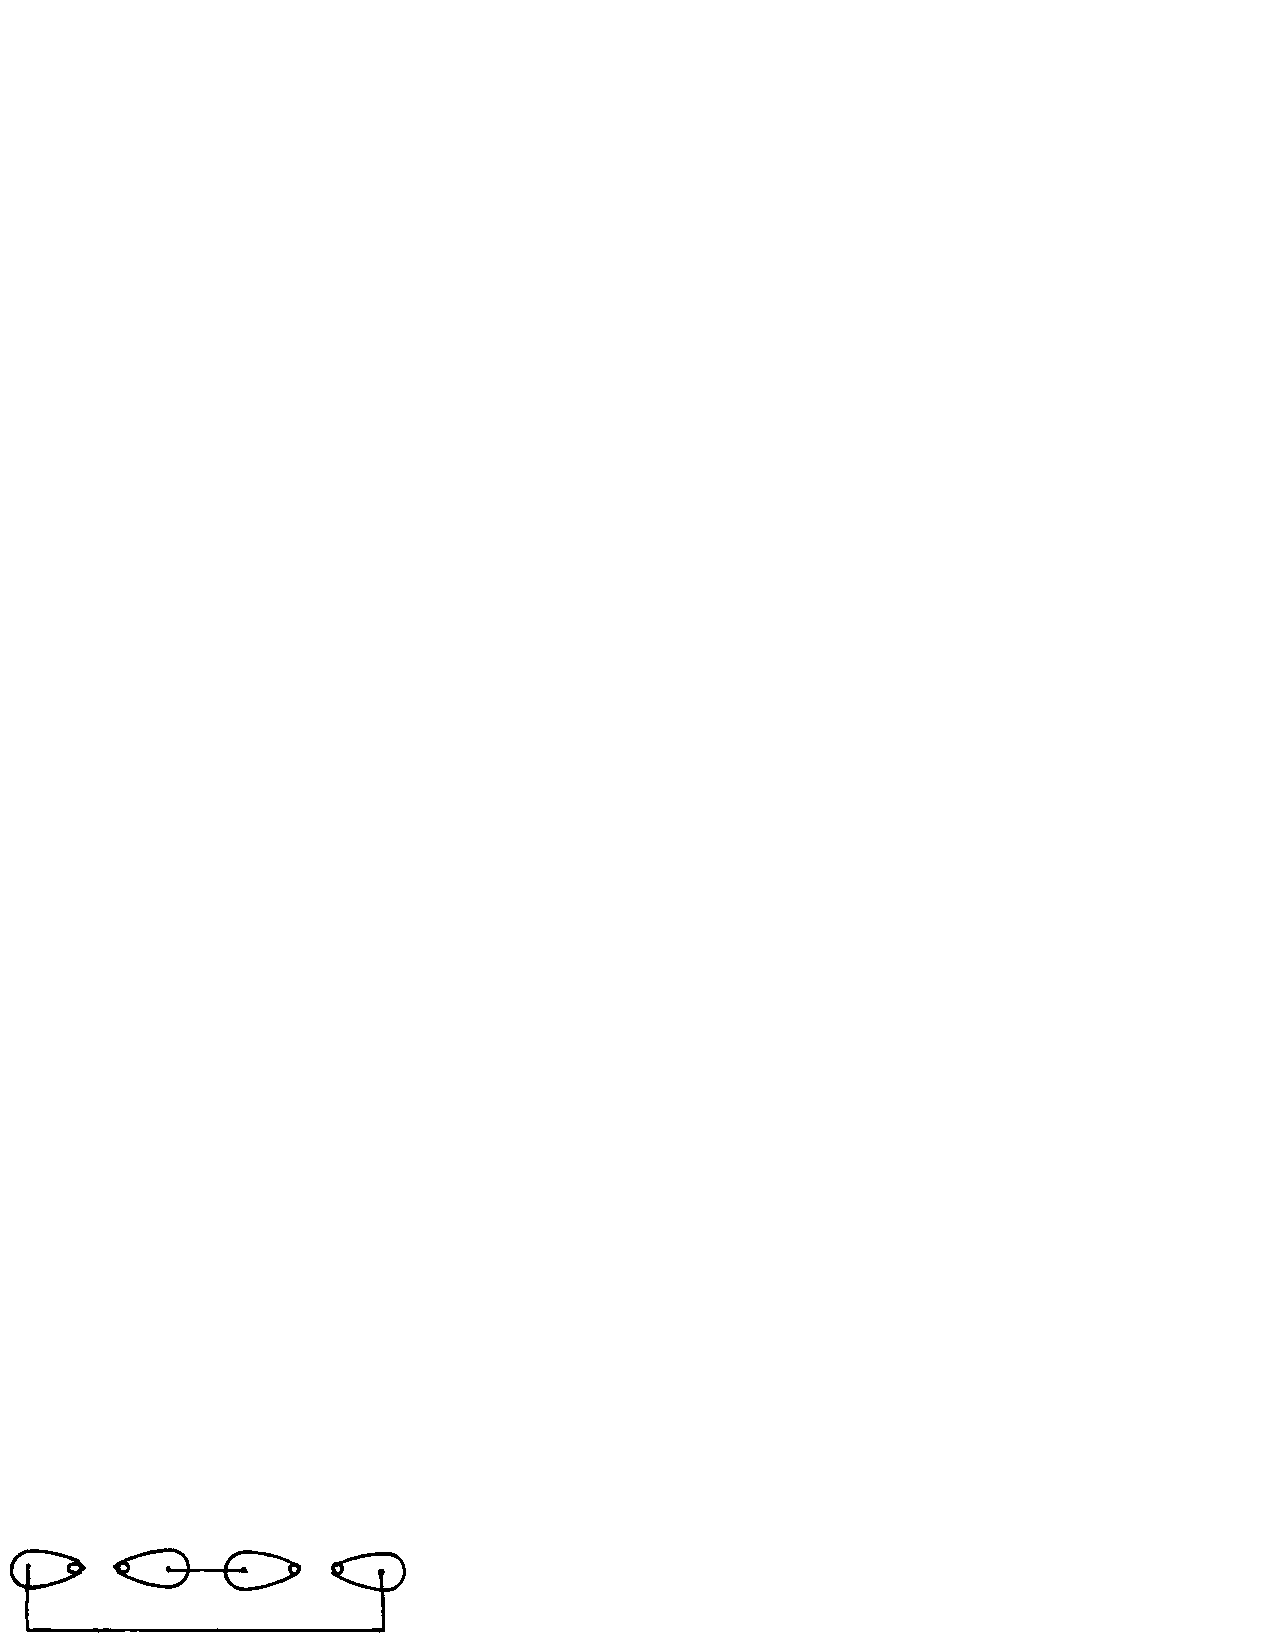
\includegraphics[scale=0.75]{fg10-8a}
\end{equation}
are shown in Figure \ref{chap10-fig9}.

\begin{figure}
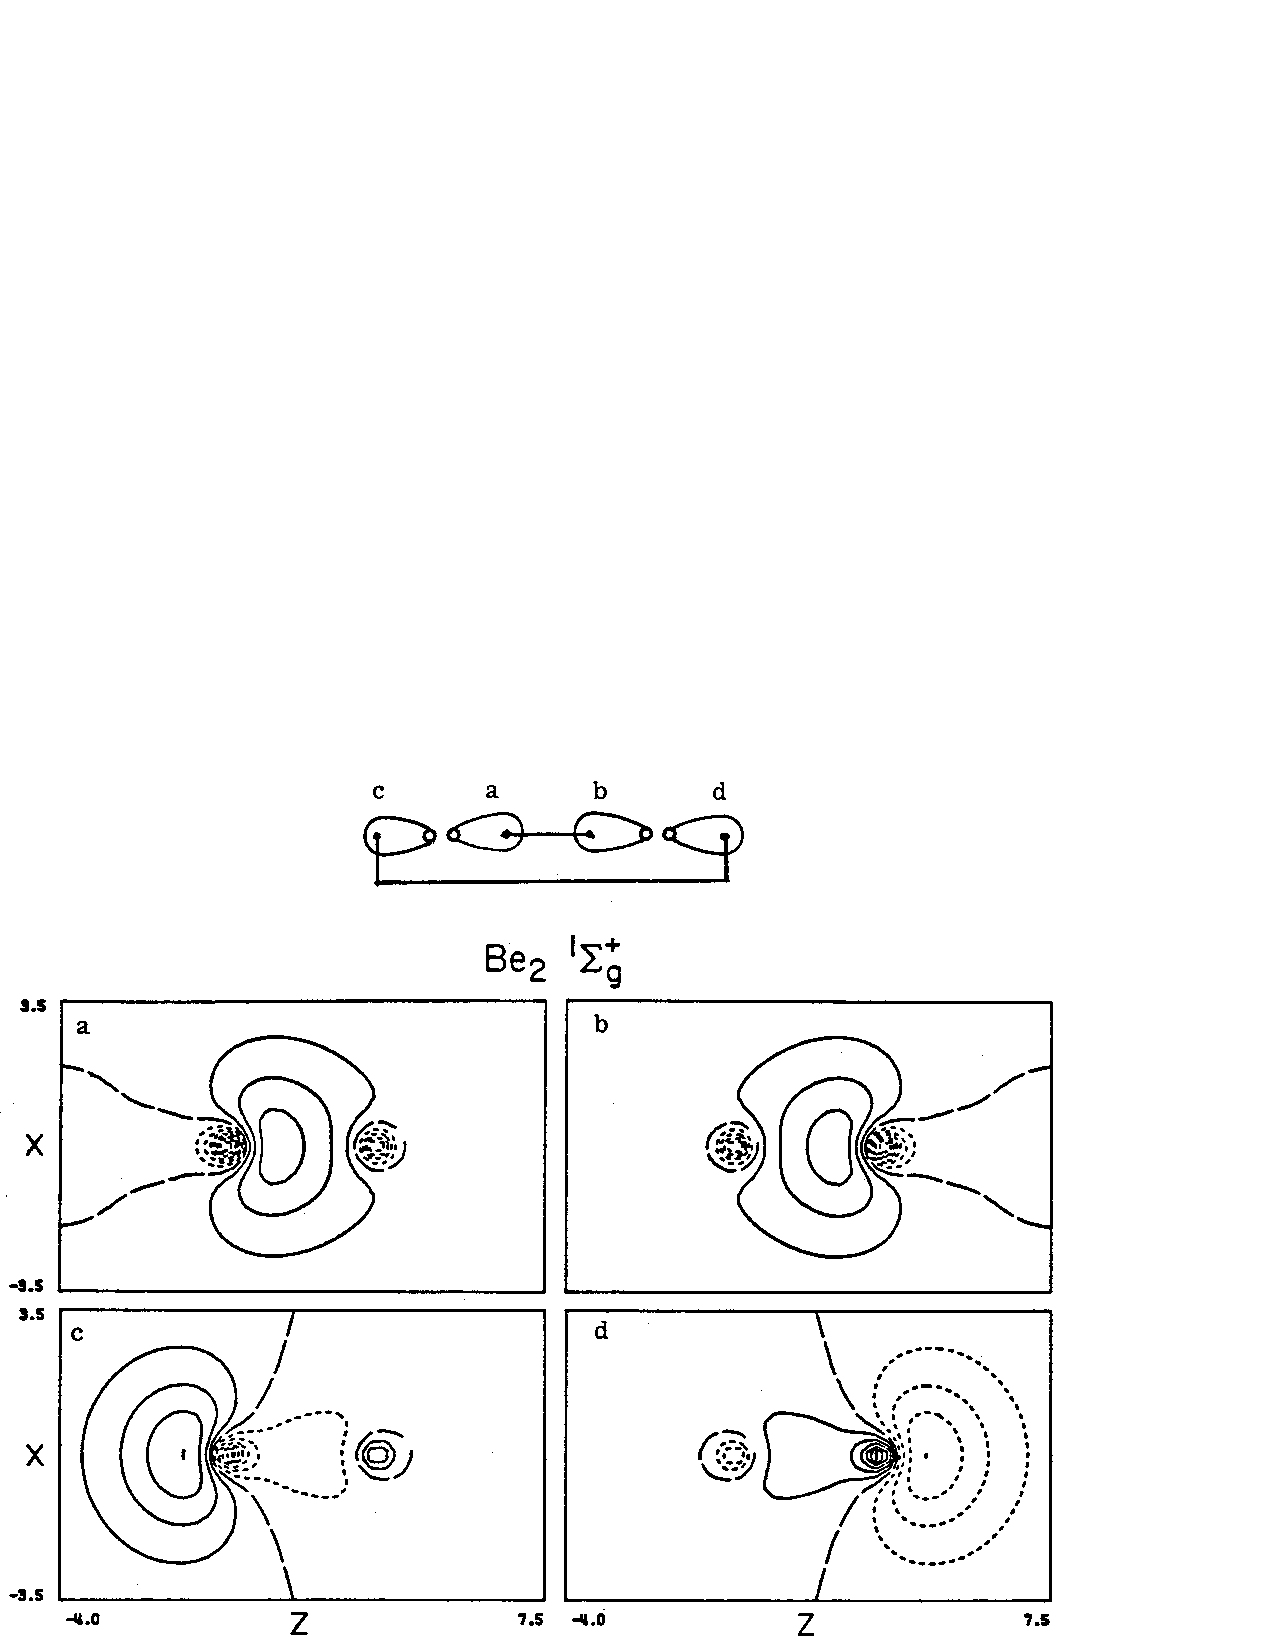
\includegraphics[scale=0.75]{fg10-9}
\caption{The GVB orbitals for the ${^1\Sigma}^+_g$ state of Be$_2$.}
\label{chap10-fig9}
\end{figure}

The MO configuration for Be$_2$ is
\begin{equation}
(1 \sigma_g )^2 (1 \sigma_u)^2 (2 \sigma_g)^2 (2 \sigma_u)^2,
\end{equation}
leading to ${^1\Sigma}^+_g$ symmetry.  Since the bonding $(2
\sigma_g)$ and antibonding $(2 \sigma_u)$ orbitals are both occupied,
they would be expected to yield a repulsive potential curve.  However,
the $2p_z$ orbitals can be used to increase the overlap for $2
\sigma_g$ (more bonding) and to decrease the overlap for $2 \sigma_u$
(less antibonding) so as to yield a net bond, but a very weak one,
$D_0 =$0. 05 eV = 1. 16 kcal.  The same is true for all elements in
the Be and Zn columns, leading to the results in Table
\ref{chap10-tab12}.  Ionizing an electron from the $2 \sigma_u$
orbital should lead to a strongly bound ${^2\Sigma}^+_u$ state, a
three-electron bond. Experimental data are not yet available.

\subsection{The B Column}

\begin{table}
\caption{Spectroscopic properties of the B$_2$ sequence.}
\label{chap10-tab13}
\begin{tabular}{cccccccc}\\ \hline
& & $R_e$ & $\omega_e$ &\multicolumn{2}{c}{$D_0$}&
\multicolumn{2}{c}{IP (eV)}\cr
& & (\AA) & (cm$^{-1}$)& (eV) & (kcal) & Molecule & Atom\cr
B$_2$ & ${^3\Sigma}^-_g$ & 1.590 & 1051.3 & 3.0$^2$ & 69.6 & & 8.296\cr
Al$_2$ & ${^3\Sigma}^-_g$ & 2.466 & 35.0 & 1.5$^5$ & 35.7 & & 5.984\cr
Ga$_2$ & & & & 1.4$^0$ & 32.3 & & 6\cr
In$_2$ & & & & 1.0$^1$ & 23.3 & & 5.785\cr
Tl$_2$ & & & & $\leq 0.9$ & $\leq 20.8$ & & 6.106\cr
\hline
\end{tabular}
\end{table}


The diatomic molecules formed from. atoms having $(ns)^2 (np)^1$
valence configurations are listed in Table \ref{chap10-tab13}. This
includes B, Al, Ga, In, and T1, but excludes Sc, Y, and La, since the
latter three elements have $(ns)^2 (n-1 d)^1$ configurations. B$_2$
leads to the strongest bond, by a factor of two, and the shortest
bond, while Ga$_2$ and Al$_2$ appear to have comparable bond energies.

For B$_2$, the lowest observed state has the MO 
configuration of
\begin{equation}
( 1 \sigma_g )^2 ( 1 \sigma_u )^2 (2 \sigma_g )^2 (2 \sigma_u )^2 
  ( 1 \pi_u )^2,
\end{equation}
leading to ${^3\Sigma}^-_g$ symmetry.  However, theoretical 
calculations$^2$ indicate that ${^5\Sigma}^-_g$ 
state arising from
\begin{equation}
( 1 \sigma_g )^2 ( 1 \sigma_u )^2 (2 \sigma_g )^2 (2 \sigma_u )^1 ( 
1 \pi_u )^2 (3 \sigma_g )^1
\end{equation}
is 0.14 eV below the lowest experimentally observed state 
${^3\Sigma}^-_g$.  Both the ${^3\Sigma}^-_g$ and ${^5\Sigma}^-_g$ 
states have the configuration of
\begin{equation}
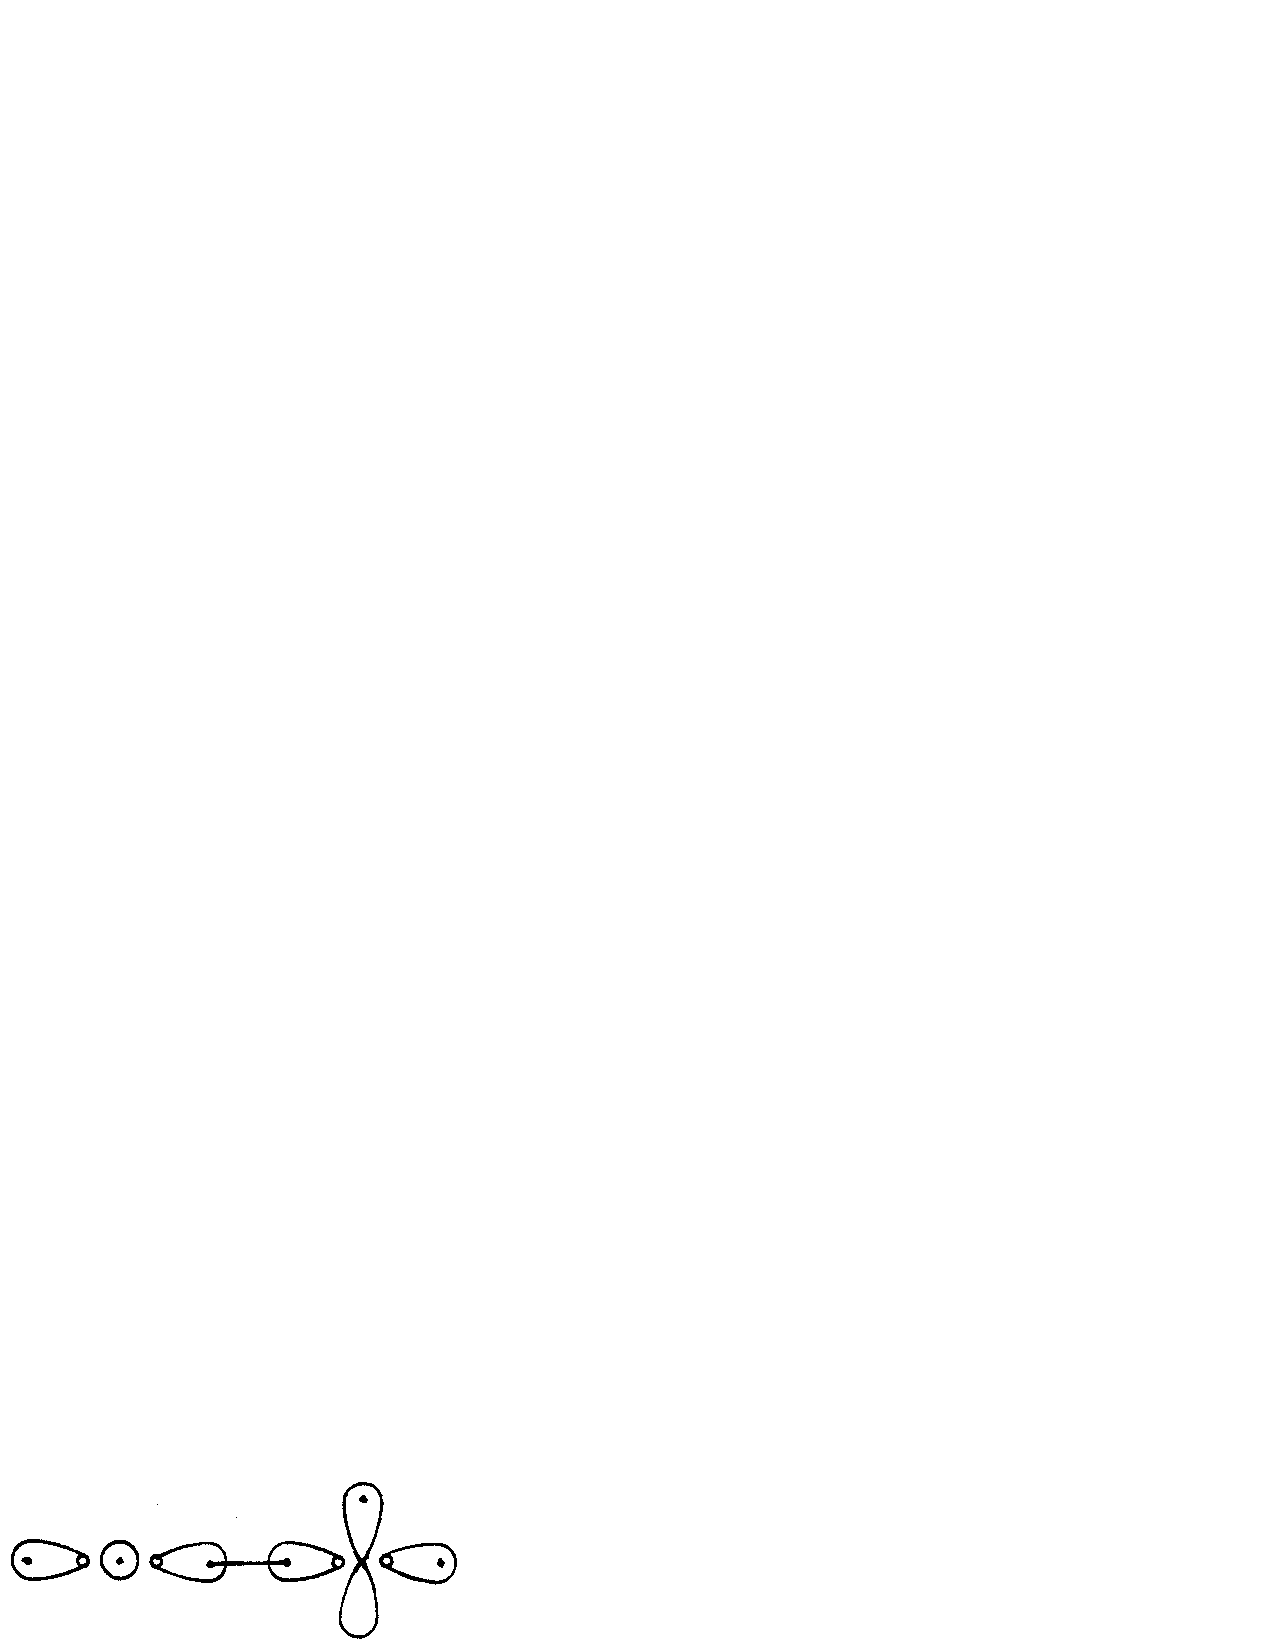
\includegraphics{fg10-9a}
\label{chap10-eqno33}
\end{equation}
However, for ${^3\Sigma}^-_g$ state, the nonbonding $\sigma$ orbitals 
are singlet paired, whereas for ${^5\Sigma}^-_g$, 
all four orbitals, excluding the bond pair, are high-spin coupled. 
Since experiments on B$_2$ are quite difficult, it could be that the 
${^5\Sigma}^-_g$ state is more stable but not identified in the 
spectrum.

The GVB orbitals for the ${^3\Sigma}^-_g$ state
of B$_2$, are shown in Figure \ref{chap10-fig10}.  Here we show only
one $\pi$ orbital, there is one in each of the xz and yz planes.
Note, in these calculations the $\pi$ orbitals are delocalized.

\begin{figure}
\includegraphics[scale=0.75]{fg10-10}
\caption{}
\label{chap10-fig10}
\end{figure}

The wavefunction should probably be a superposition of
\begin{equation}
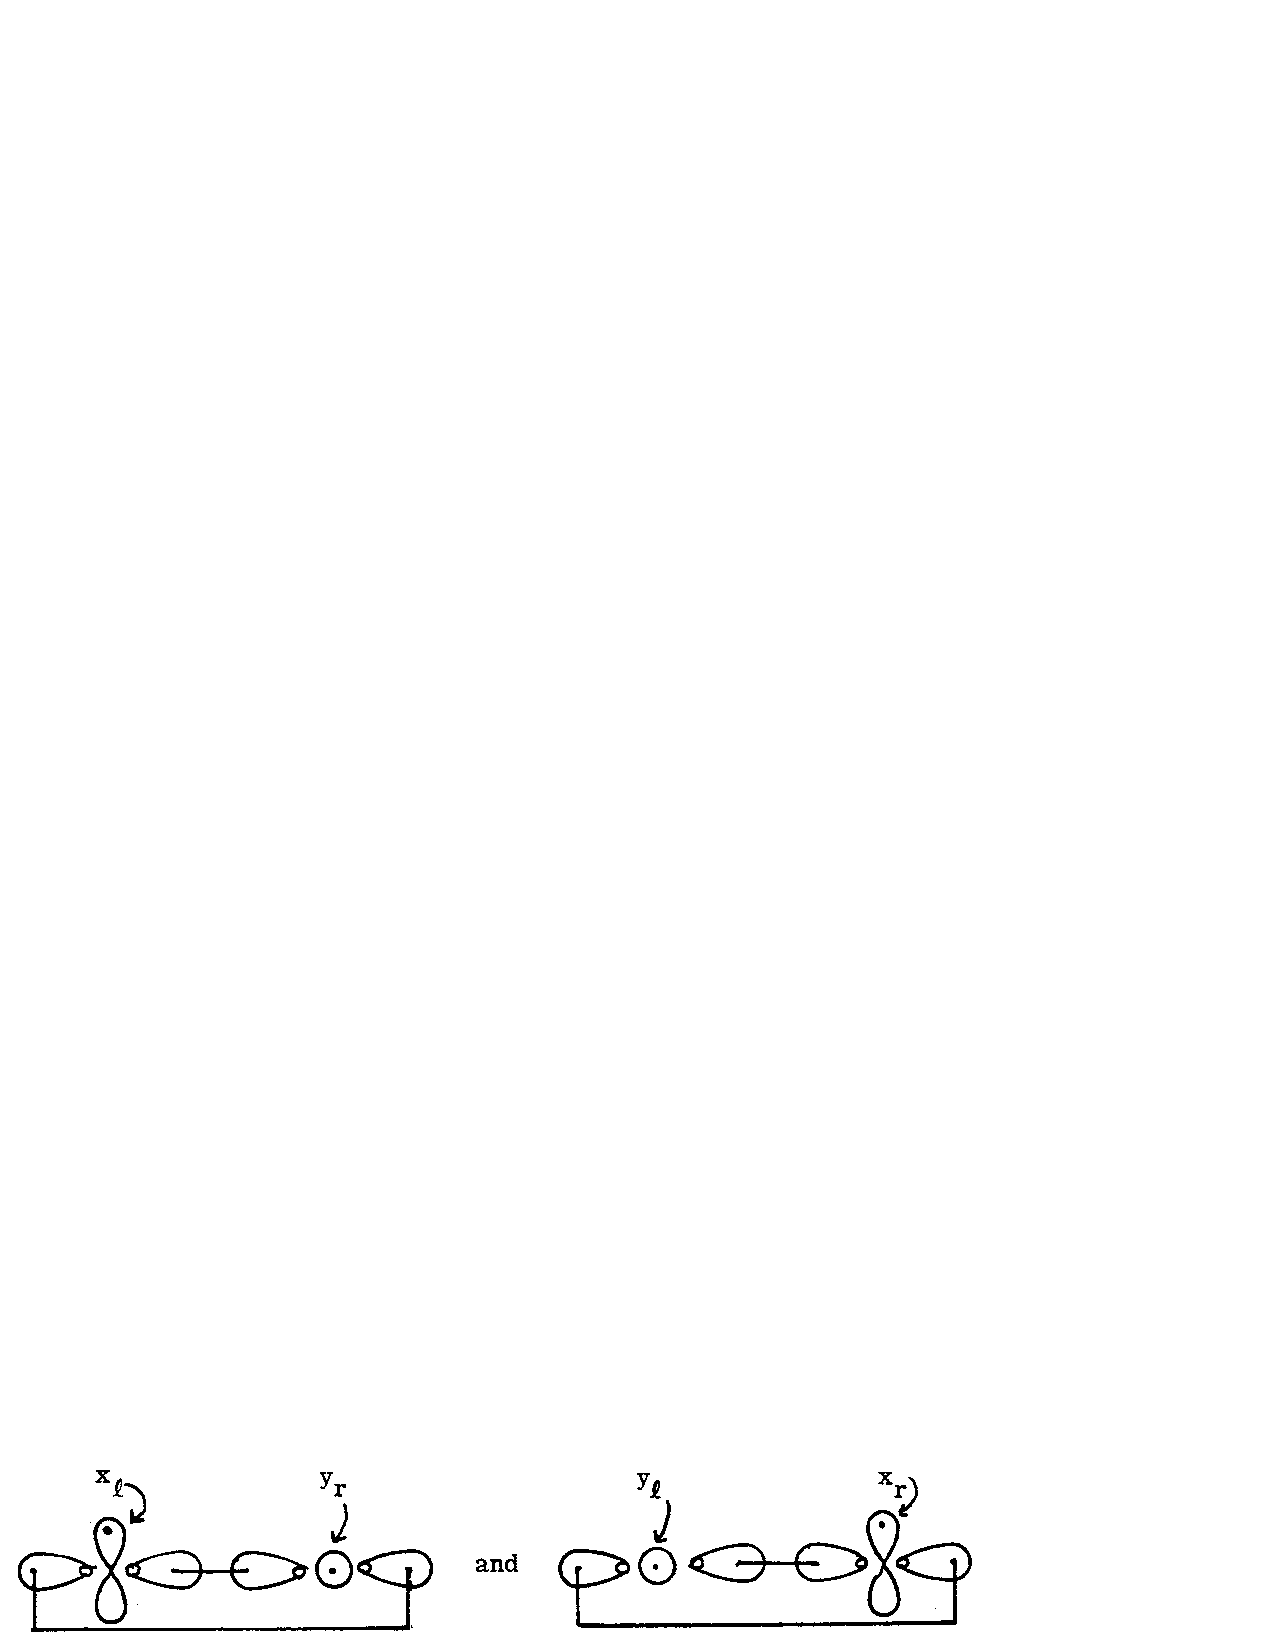
\includegraphics[scale=0.75]{fg10-9b}
\end{equation}
i.e., the $\pi$ system should be
\begin{equation}
{\cal A} \left( x_l x_r + y_l x_r \right) \alpha \alpha
\end{equation}
however, the calculations leads to
\begin{equation}
{\cal A} \left[ \pi_{xu} \pi_{yu} \alpha \alpha \right] .
\end{equation}

\subsection{The C Column}

\begin{table}
\caption{Spectroscopic properties of the C$_2$ sequence.}
\label{chap10-tab14}
\begin{tabular}{cccccccc}\\ \hline

& & $R_e$ & $\omega_e$ &\multicolumn{2}{c}{$D_0$}&
\multicolumn{2}{c}{IP}\cr
& & (\AA) & (cm$^{-1}$) & (eV) & (kcal) & Molecule & Atom\cr
C$_2$ & ${^1\Sigma}^+_g$ & 1.2425 & 1854.7 & 6.21 & 143.2 & 12.15 & 
10.256\cr
Si$_2$ & ${^3\Sigma}^-_g$ & 2.246 & 511.0 & 3.21 & 74.0 & & 8.149\cr
Ge$_2$ & & & & 2.8$^2$ & 65.0 & & 7.8\cr
Sn$_2$ & & & & 1.9$^9$ & 45.9 & & 7.342\cr
Pb$_2$ & & & & 0.8$^2$ & 18.9 & & 7.415\cr
C$_2^+$ & ${^2\Pi}_u$ & [1.301] & (1350) & 5.3$^2$ & 122.7\cr
C$^-_2$ & ${^2\Sigma}^+_g$ &1.2682 & 1781.0 & 84$^8$ & 195.5 & 3.54 & 
1.268\cr 
SiC & ${^3\Pi}_i$ & (1.82) & (9.83) & 4.6$^4$ \cr
GeC & & & & 4.7$^3$\cr
GeSi & & & & 3.0$^8$\cr
\hline
\end{tabular}
\end{table}

The properties of C$_2$, Si$_2$, Ge$_2$, Sn$_2$, and Pb$_2$ 
are summarized in Table \ref{chap10-tab14}.  Of these,
only C$_2$ and Si$_2$ are well studied.  Particularly relevant to note is
that the ground state of C$_2$ is a ${^1\Sigma}^+_g$ state, instead 
of ${^3\Sigma}^-_g$ as for Si$_2$.

\subsubsection{C$_2$}

\begin{table}
\caption{Low-lying state of C$_2$.}
\label{chap10-tab15}
\begin{tabular}{cccccccc}\\ \hline

 & Energy (eV)& $R_e$ (\AA)& $\omega_e$ (cm$^{-1}$) & $2\sigma_g$ &
    $2\sigma_u$ & $1\pi_u$ & $3\sigma_g$\cr

 ${^3\Sigma}^+_u$ & 1.6505 & 1.23 & 1961.6 & 2 & 1 & 4 & 1\cr
 ${^1\Sigma}^+_g$ & 0.0 & 1.2425 & 1854.7 & 2 & 2 & 4 & 0\cr
 ${^1\Sigma}^+_g$ &\cr
 ${^1\Delta}_g$ &\cr
 ${^3\Sigma}^-_g$ & 0.7978 & 1.3693 & 1470.5 & 2 & 2 & 2 & 2\cr

 ${^1\Pi}_u$ & 1.0404 & 1.3184 & 1608.4 & 2 & 2 & 3 & 1\cr
 ${^3\Pi}_u$ & 0.0888 & 1.3119 & 1641.4 & 2 & 2 & 3 & 1\cr
\hline
\end{tabular}
\end{table}

The three important bonding configurations for C$_2$, are shown in Table 
\ref{chap10-tab15}.  The two major factors in
changing the ground configuration are 
\begin{enumerate}
\item C$_2$ makes much stronger pi bonds than Si$_2$. 
\item It is easier to use the $2s$ lobe pair of C in bonds than the
$3s$ lobe pair of Si. 
\end{enumerate}
Note that the ${^3\Pi}_u$ state of C$_2$ is only 0.09 eV above the
ground state, ${^1\Sigma}^+_g$.  Indeed, until 1962, the experimental
ground state of C$_2$ was the ${^3\Pi}_u$ state.  On the other hand,
for SiC, the ${^3\Pi}$ state is the ground state.

Note that states with the same valence bond configuration lead to
similar properties.  Thus, configuration equation
(\ref{chap10-eqno33}), with a triple bond
\begin{equation}
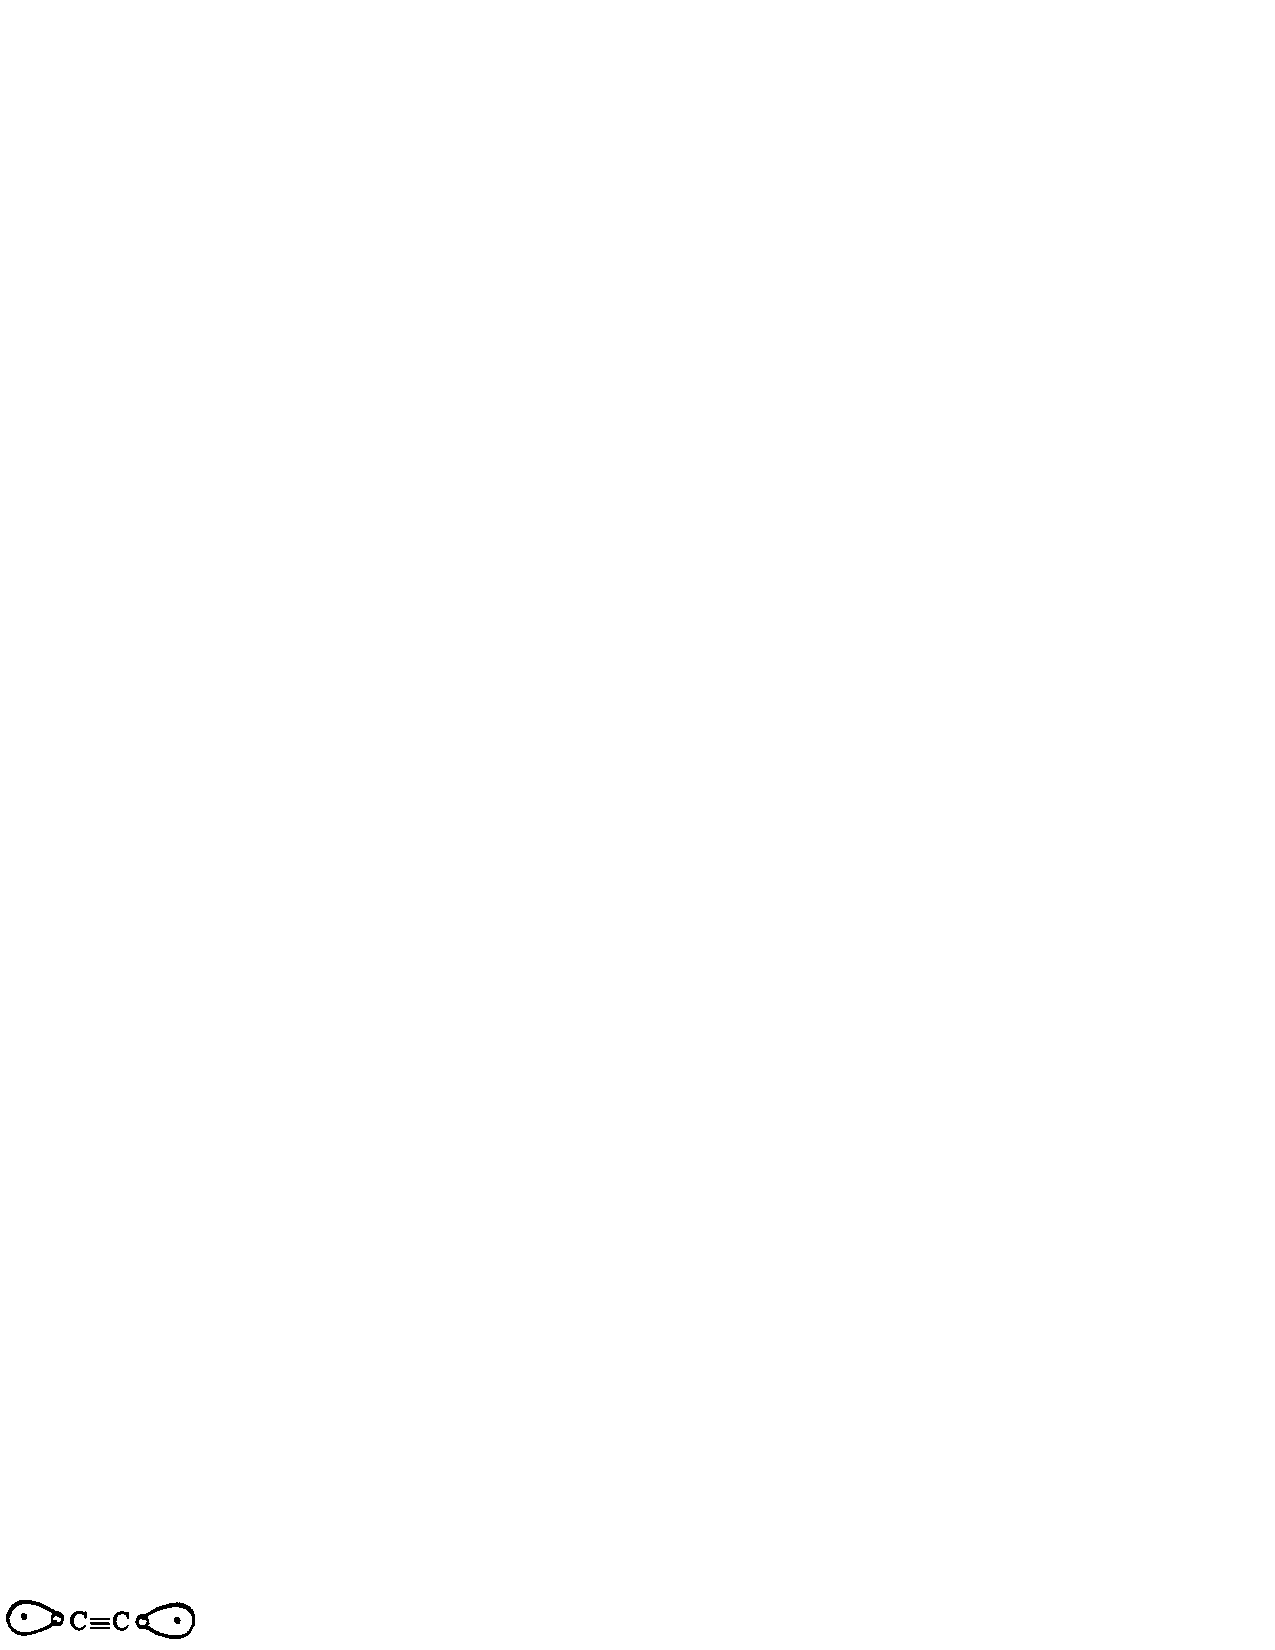
\includegraphics{fg10-10b}
\end{equation}
leads to $R_e = 1.23$ and 1. 24 \AA, and $\omega_0 = 1962$ and 1855 
cm$^{-1}$ for the ${^3\Sigma}^+_u$ and ${^1\Sigma}^+_g$ state, 
respectively, despite the 1.65 eV separation between these
states.  Indeed, these properties are close to those of acetylene, 
HCCH, also possessing a triple bond $R_{CC} =$ 1.208\AA, 
and $\omega_{CC} = 1974$ cm$^{-1}$.  On the other hand, the MO
configurations are different 
\begin{eqnarray}
{^1\Sigma}^+_g &:&\left( \sigma_g 2s \right)^2 \left( \sigma_u 2s 
\right)^2 \left( 1 \pi_u \right)^4\\
{^3\Sigma}^+_u &:& \left( \sigma_g 2s \right)^2 \left( \sigma_u 2s 
\right)^1 \left( 1 \pi_u \right)^4 \left( \sigma_g 2p \right)^1
\label{chap10-eqno34}
\end{eqnarray}
The other MO configurations are
\begin{eqnarray}
{^3\Sigma}^-_g &:& \left( \sigma_g 2s \right)^2 \left( \sigma_u 2s 
\right)^2 \left( \sigma_g 2p \right)^2 \left( \pi_u \right)^2\\
{^3\Pi}^-_u &:& \left( \sigma_g 2s \right)^2 \left( \sigma_u 2s 
\right)^2 \left( \sigma_g 2p \right)^1 \left( 1 \pi_u \right)^3
\end{eqnarray}
Based on the valence bond diagrams, we observe that
\begin{enumerate}
\item ${^3\Sigma}^-_g$ has a two-electron $\sigma$ bond and
two one-electron bonds for a final bond order of 2,
\item ${^3\Pi}_u$ has a two-electron $\sigma$ bond, a two-electron
$\pi$ bond,  and a one-electron $\pi$ bond for a final
bond order of 2-1.2. 
\item ${^1\Sigma}^+_g$ has a final bond 
order of 3. 
\end{enumerate}
Indeed, the bond length decreases from 1.37 to 1.31 to 1.24 \AA, and
the vibrational frequency increases from 1470 to 1641 to 1855
cm$^{-1}$ as the bond order increases from 2 to 2-1/2 to 3.  The
orbitals for the ${^1\Sigma}^+_2$ and ${^3\Pi}$ states, of C$_2$, are
shown in Figures \ref{chap10-fig11} and \ref{chap10-fig12}

\begin{figure}
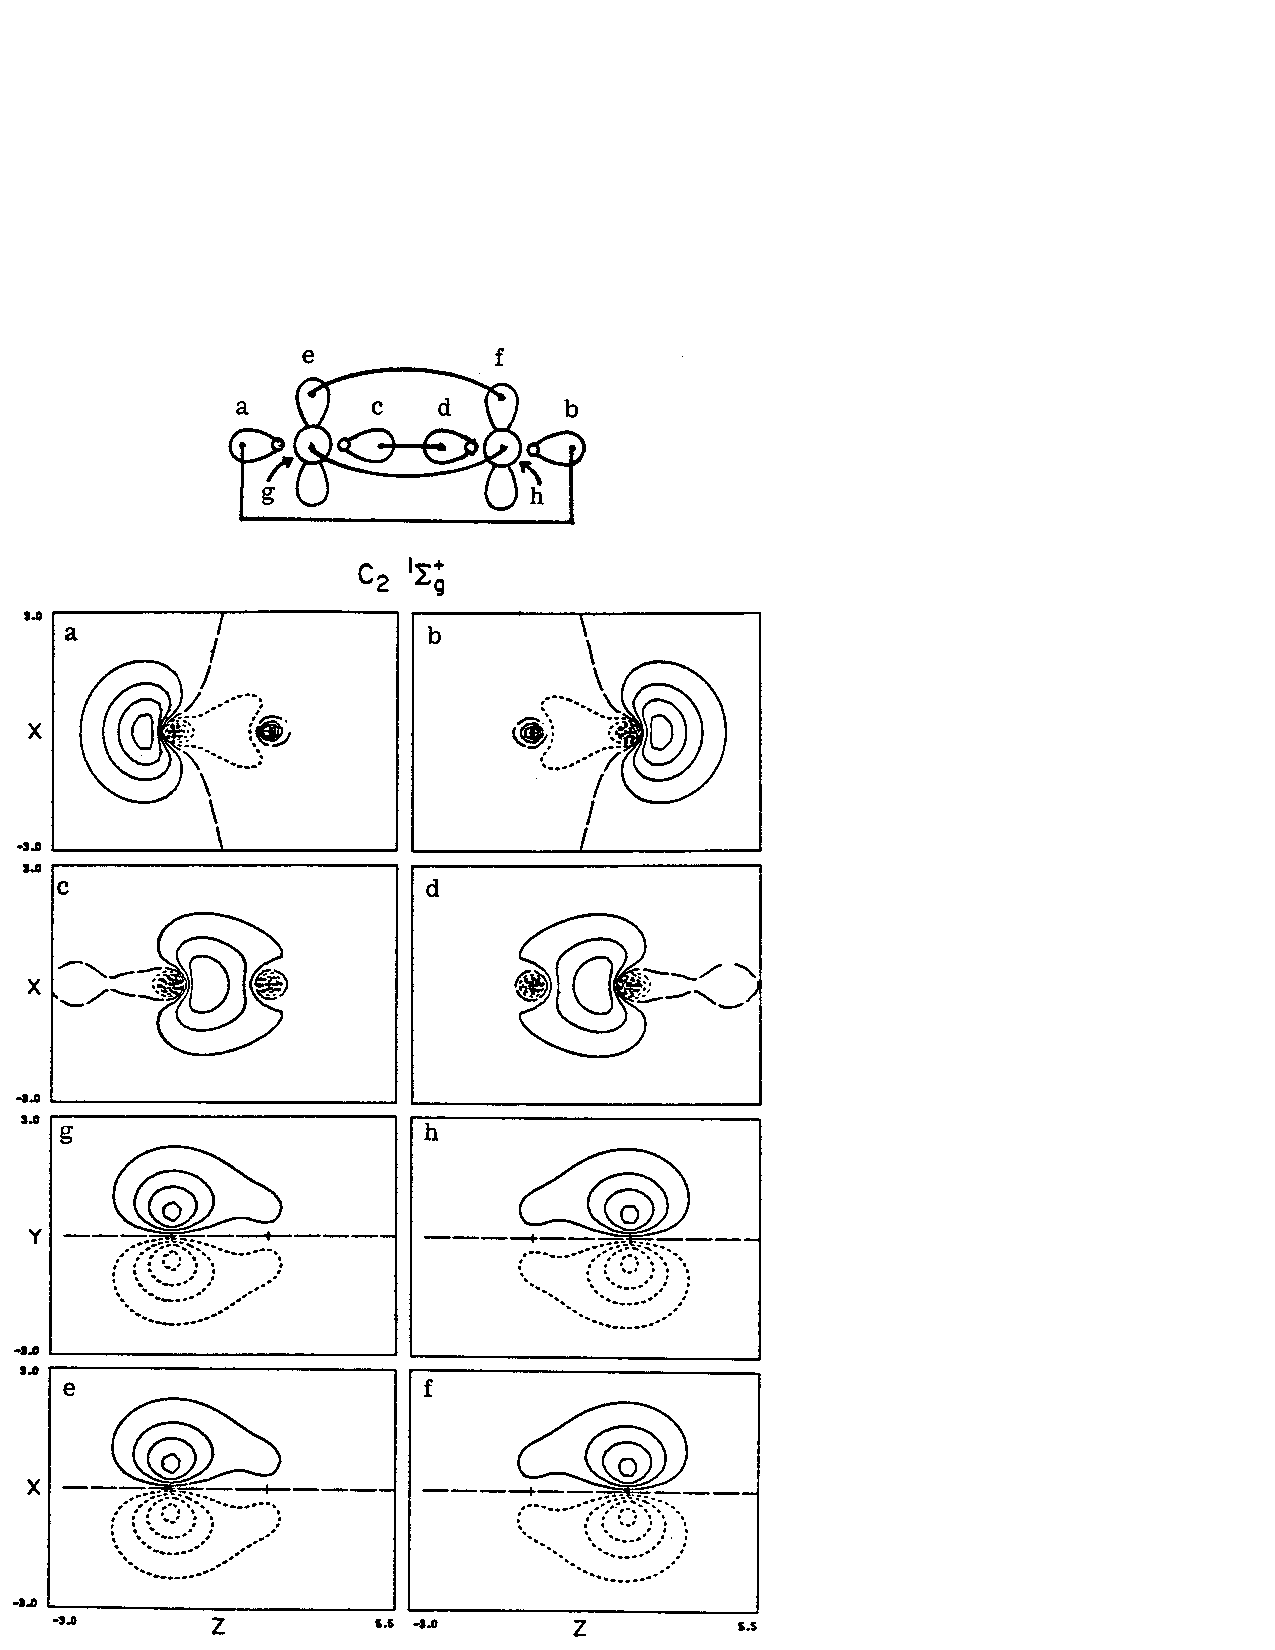
\includegraphics[scale=0.75]{fg10-11}
\caption{GVB orbitals for the ${^1\Sigma}^+$ state of C$_2$.}
\label{chap10-fig11}
\end{figure}


\begin{figure}
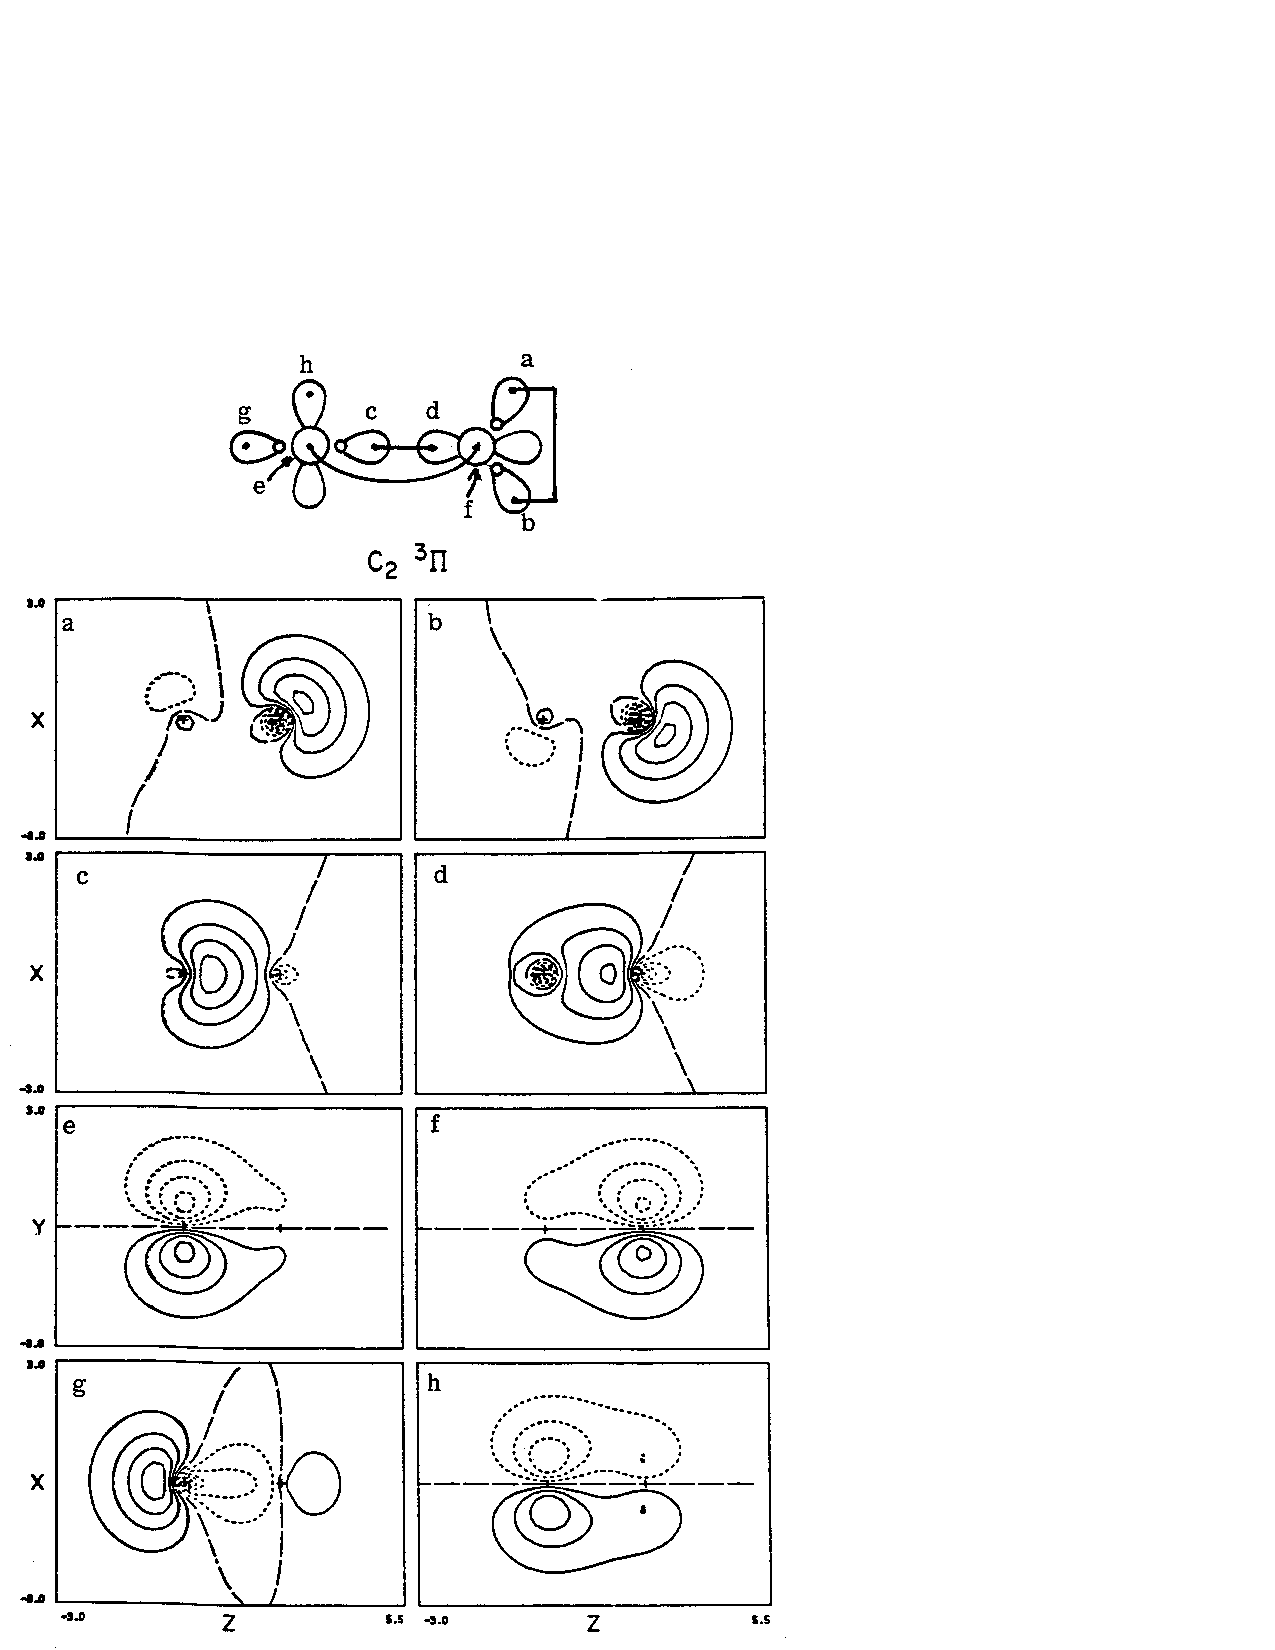
\includegraphics[scale=0.75]{fg10-12}
\caption{GVB orbitals for the 
${^3\Pi}$ state of C$_2$.  Note that the orbitals are not symmetry
functions.  This wavefunction is combined with the reflected one to
lead to ${^3\Pi}_u$, lower, and ${^3\Pi}_g$, higher, states.  }
\label{chap10-fig12}
\end{figure}



\subsubsection{C$^-_2$ and C$^+_2$}

Starting with the MO configuration in equation (\ref{chap10-eqno34}),
for the ground state of C$_2$, we would expect C$^+_2$ to have the
configuration
\begin{equation}
{^2\Pi}_u \left( \sigma_g 2s \right)^2 \left( \sigma_u 2s \right)^2 
\left( 1 \pi_u \right)^3
\end{equation}
and C$^-_2$ to have the configuration
\begin{equation}
{^2\Sigma}_g \left( \sigma_g 2s \right)^2 \left( \sigma_u 2s \right)^2 
\left( 1 \pi_u \right)^4 \left( \sigma_g 2p \right)
\end{equation}
Since $1 \pi_u$ and $\sigma_g 2p$ are of bonding character, the bond
energies should increase as we proceed from C$^+_2$ to C$_2$ to
C$^-_2$. Indeed, this is observed, see Table \ref{chap10-tab16}.
However, the sequence is not smooth, C$^-_2$ is 30 \% more
strongly bonding than C$_2$.  In addition, the trend in $R_e$ and
$\omega_e$ is not exactly what would be expected.

\begin{table}
\caption{}
\label{chap10-tab16}
\begin{tabular}{ccccc}\\ \hline
& Symmetry & $R_e$ (\AA) & $\omega_e$  (cm$^{-1}$) & $D_0$ (kcal)\cr
C$^+_2$ & ${^2\Pi}_u$ & [1.301] & (1350) & 122.7\cr
C$_2$ & ${^1\Sigma}^+_g$ & 1.243 & 1855	 & 143.2\cr
C$^-_2$ & ${^2\Sigma}^+_2$ & 1.268 & 1781 & 195.5\cr
\hline
\end{tabular}
\end{table}

In the VB model we would represent these species as
\begin{equation}
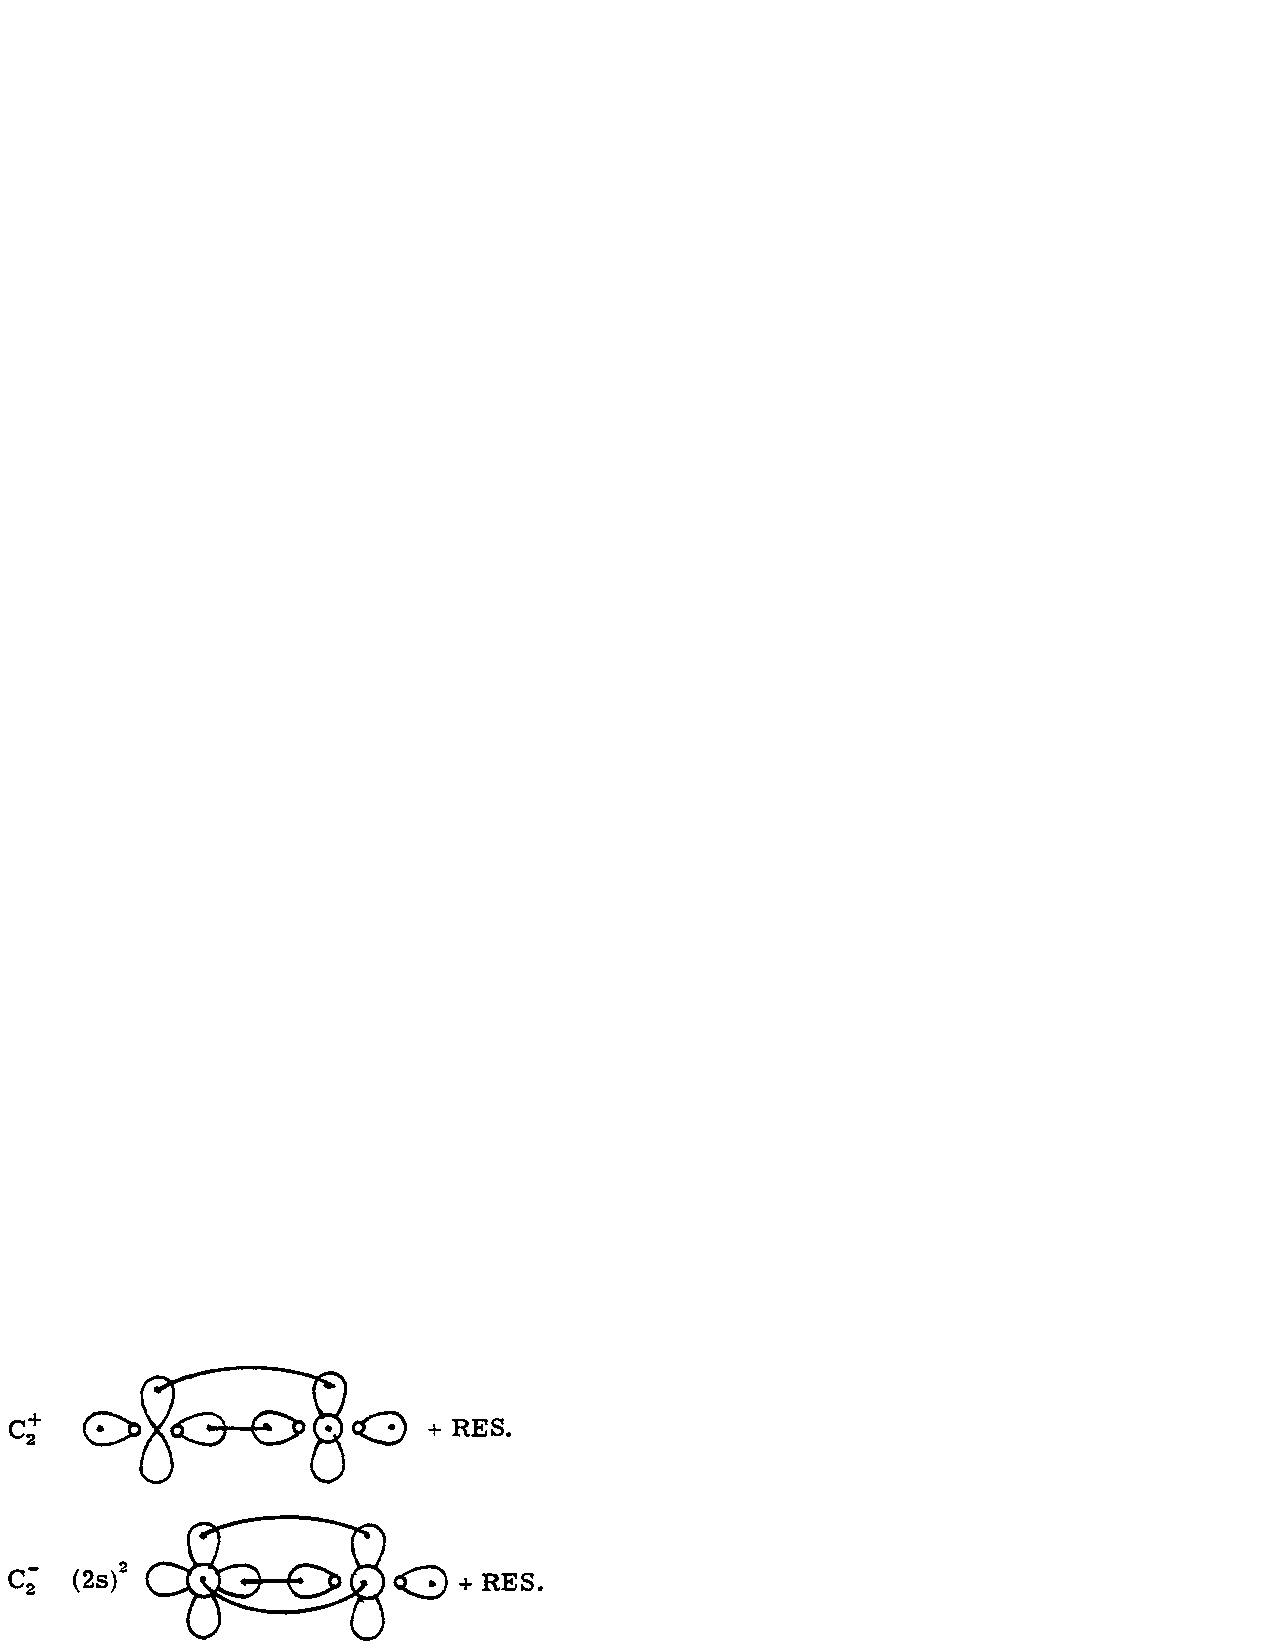
\includegraphics{fg10-12a}
\end{equation}
Thus, the special aspect of C$^-_2$ is that the C$^-$ fragment is
\begin{equation}
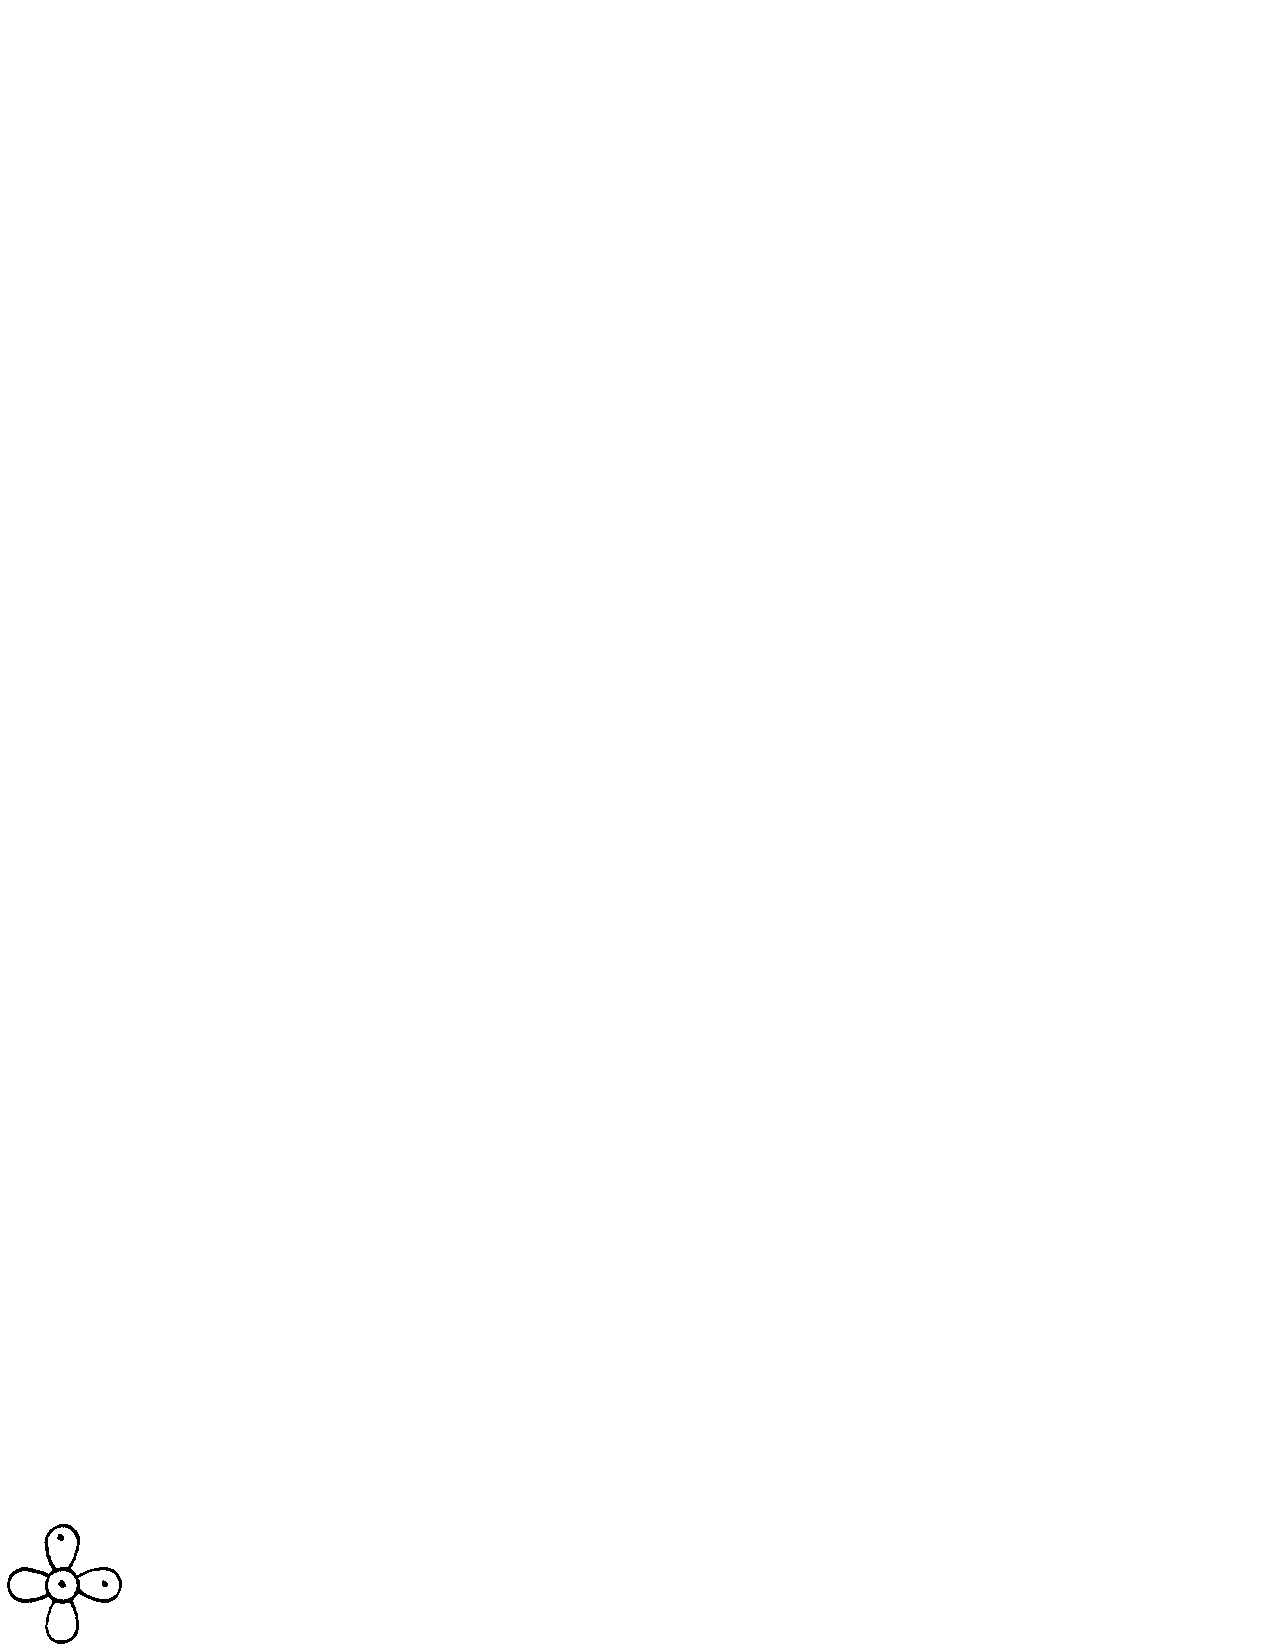
\includegraphics{fg10-12b}
\end{equation}
with an uncorrelated $2s$ pair. Thus, in forming the bond, we need not unpair
the $2s$ pair, leading to a stronger bond than might be expected from 
comparison to C$^+_2$ and C$_2$.

\subsection{The N Column}

\subsubsection{Neutrals}

The elements N, P, As, Sb, and Bi all have a $(ns)^2 (np)^3$ valence 
configuration and, thus, should lead to a triple bond
\begin{equation}
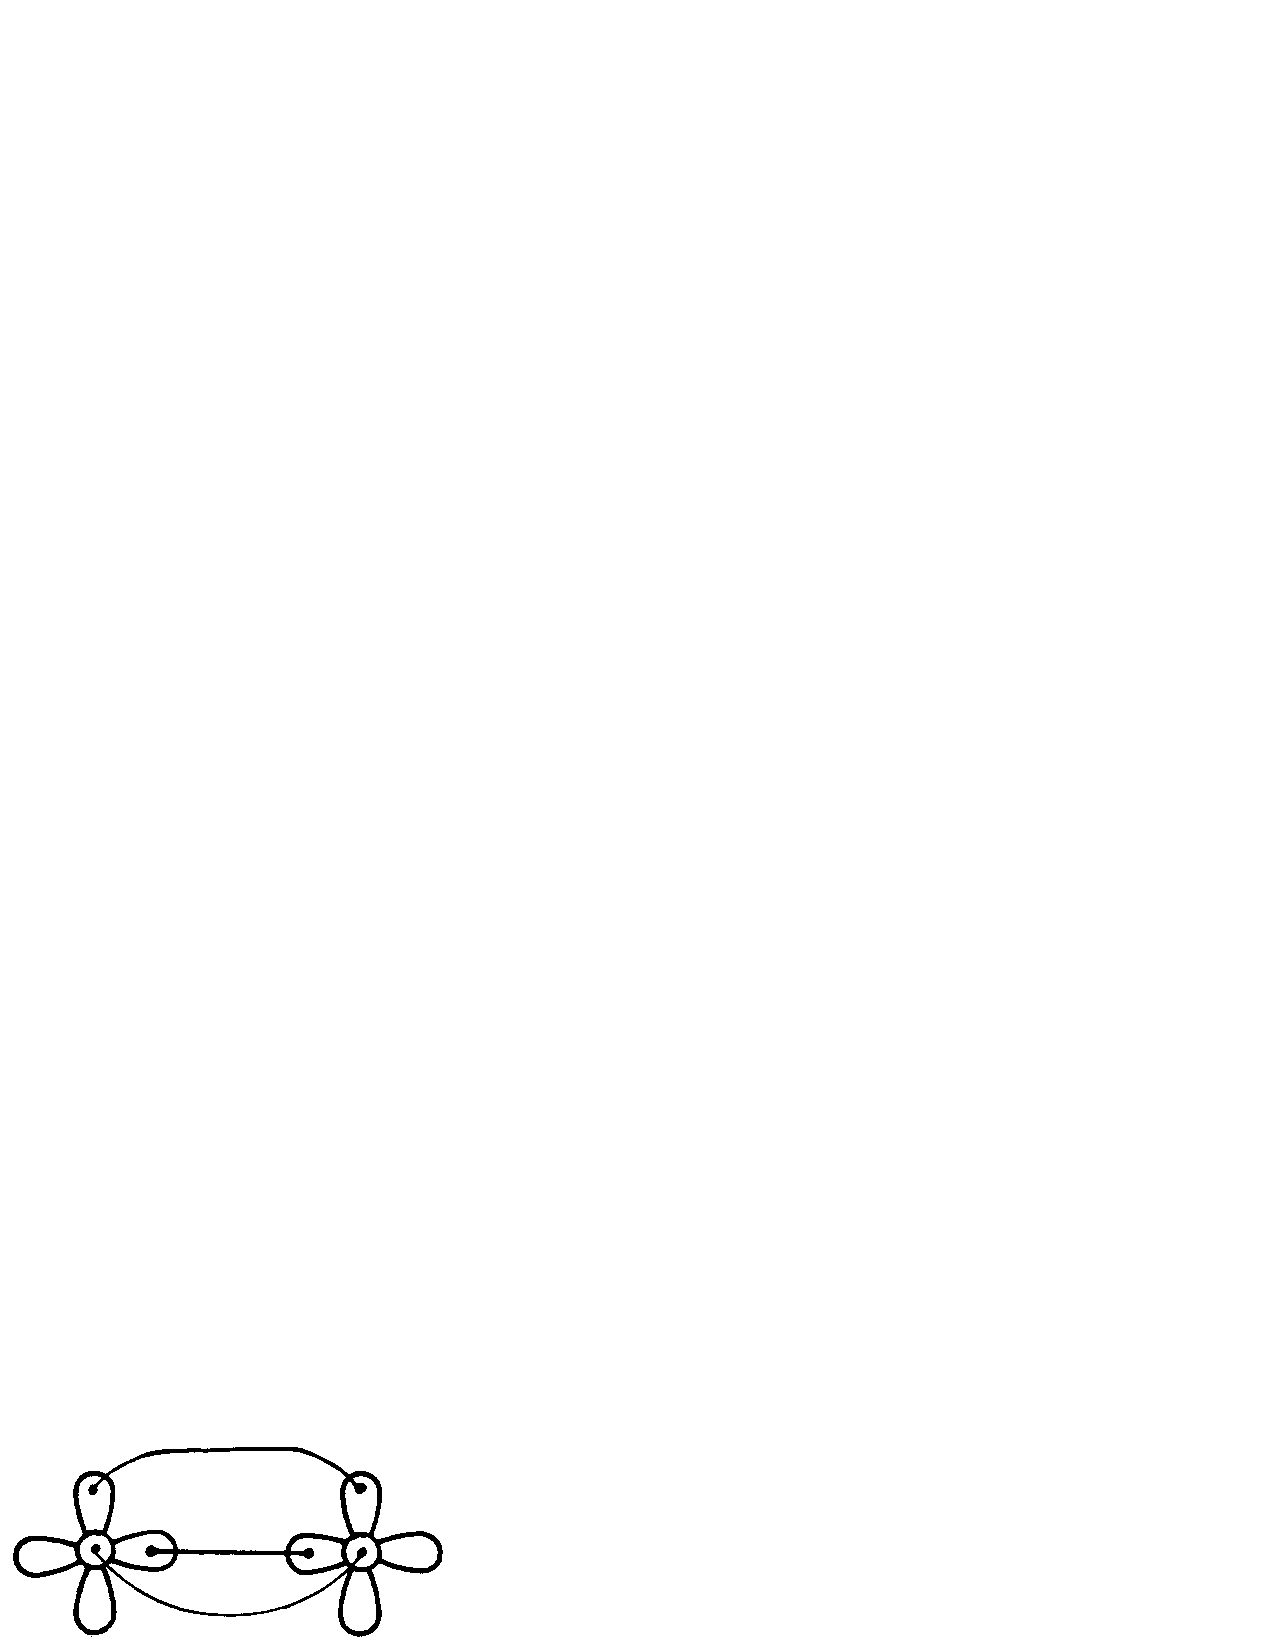
\includegraphics{fg10-12c}
\end{equation}
Adding in the $ns$ pairs, we might indicate this wavefunction as
\begin{equation}
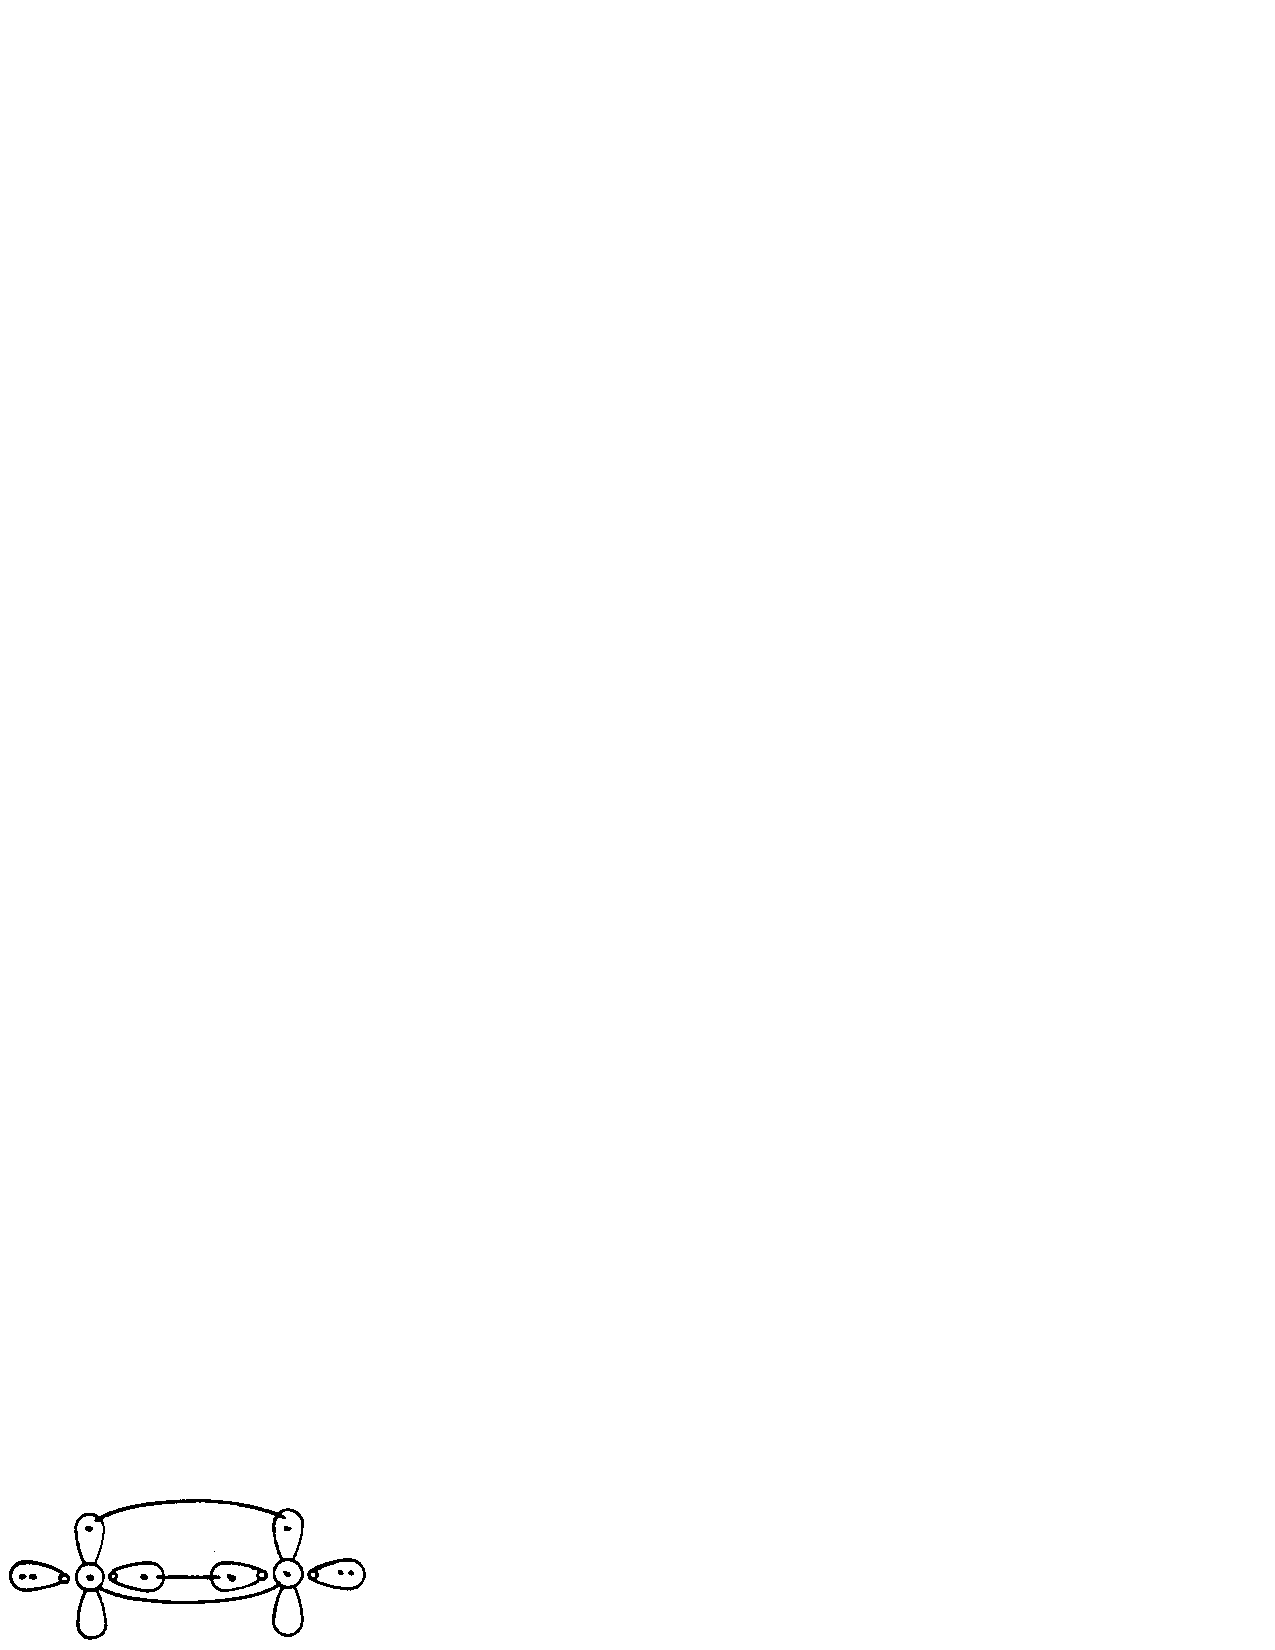
\includegraphics{fg10-12d}
\label{chap10-eqno35}
\end{equation}
This is the valence bond description of N$_2$, etc.  The optimum
orbitals of N$_2$ are shown in Figure \ref{chap10-fig13} for various
internuclear distances.


\begin{figure}
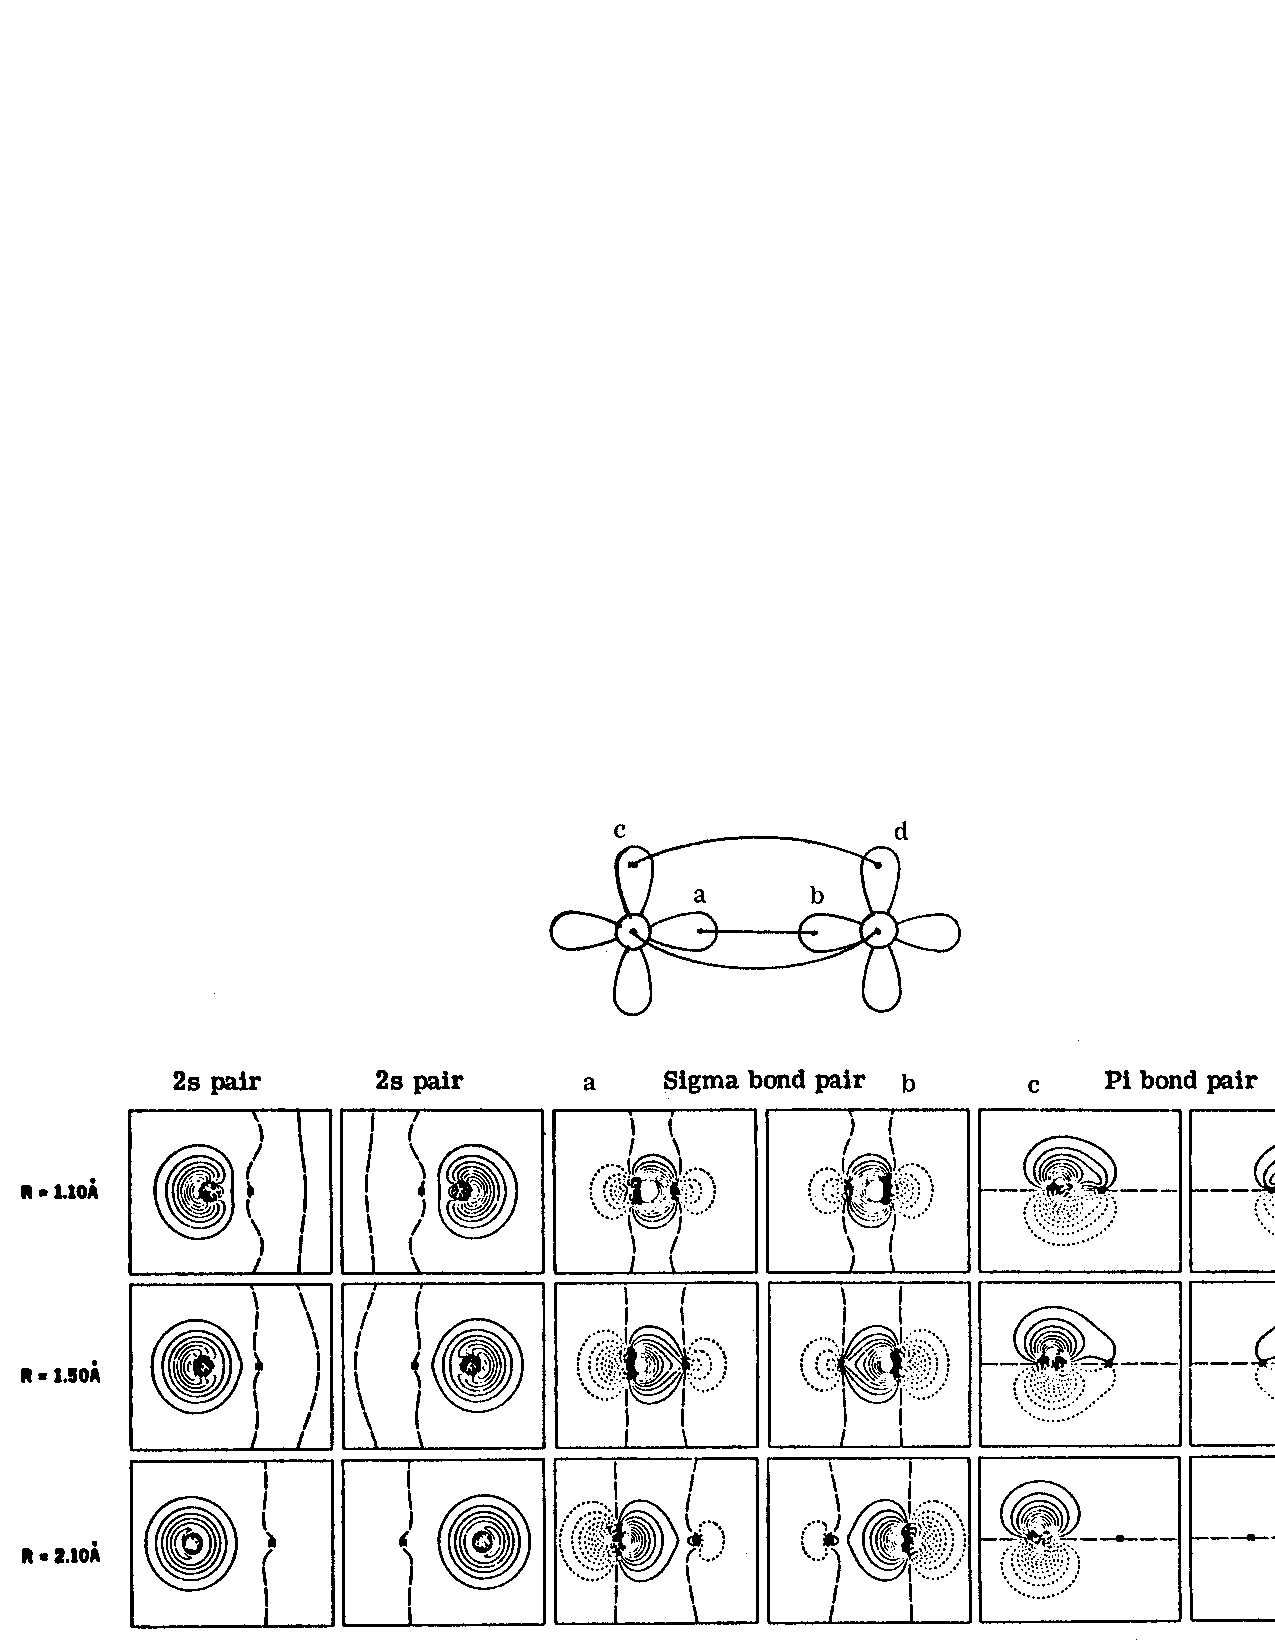
\includegraphics[scale=0.75,angle=90]{fg10-13}
\caption{GVB orbitals of the N$_2$, X ${^1\Sigma}^+_2$, molecule for
various $R$.}
\label{chap10-fig13}
\end{figure}

\begin{table}
\caption{}
\label{chap10-tab17}
\begin{tabular}{cccc}\\ \hline
& $R_e$ (\AA)& $\omega_e$ (cm$^{-1}$) & $D_0$ (kcal)\cr
N$_2$ & 1.10 & 2359 & 225\cr
P$_2$ & 1.89 & 781 & 116\cr
As$_2$ & 2.10 & 430 & 91\cr
Sb$_2$ & 2.34 & 270 & 71\cr
Bi$_2$ & 2.66 & 173 & 47\cr
\hline
\end{tabular}
\end{table}

For N$_2$, the MO description, Table
\ref{chap10-tab17}, leads to
\begin{equation}
\underbrace{(1 \sigma_g)^2(2 \sigma_g)^2}_{N~1s~core~orbitals} 
\underbrace{(2 \sigma_g)^2 (2 \sigma_u)^2}_{N~2s~lone~pairs} 
\underbrace{(1 \pi_{ux})^2 (1 \pi_{uy})^2 (3 
\sigma_g)^2}_{triple~bond}
\end{equation}
with orbitals that correspond closely to those in the GVB 
wavefunction.  In either description, there is a triple bond 
leading to a very strong, short bond.  The HF orbitals 
are shown in Figure \ref{chap10-fig14}.

\begin{figure}
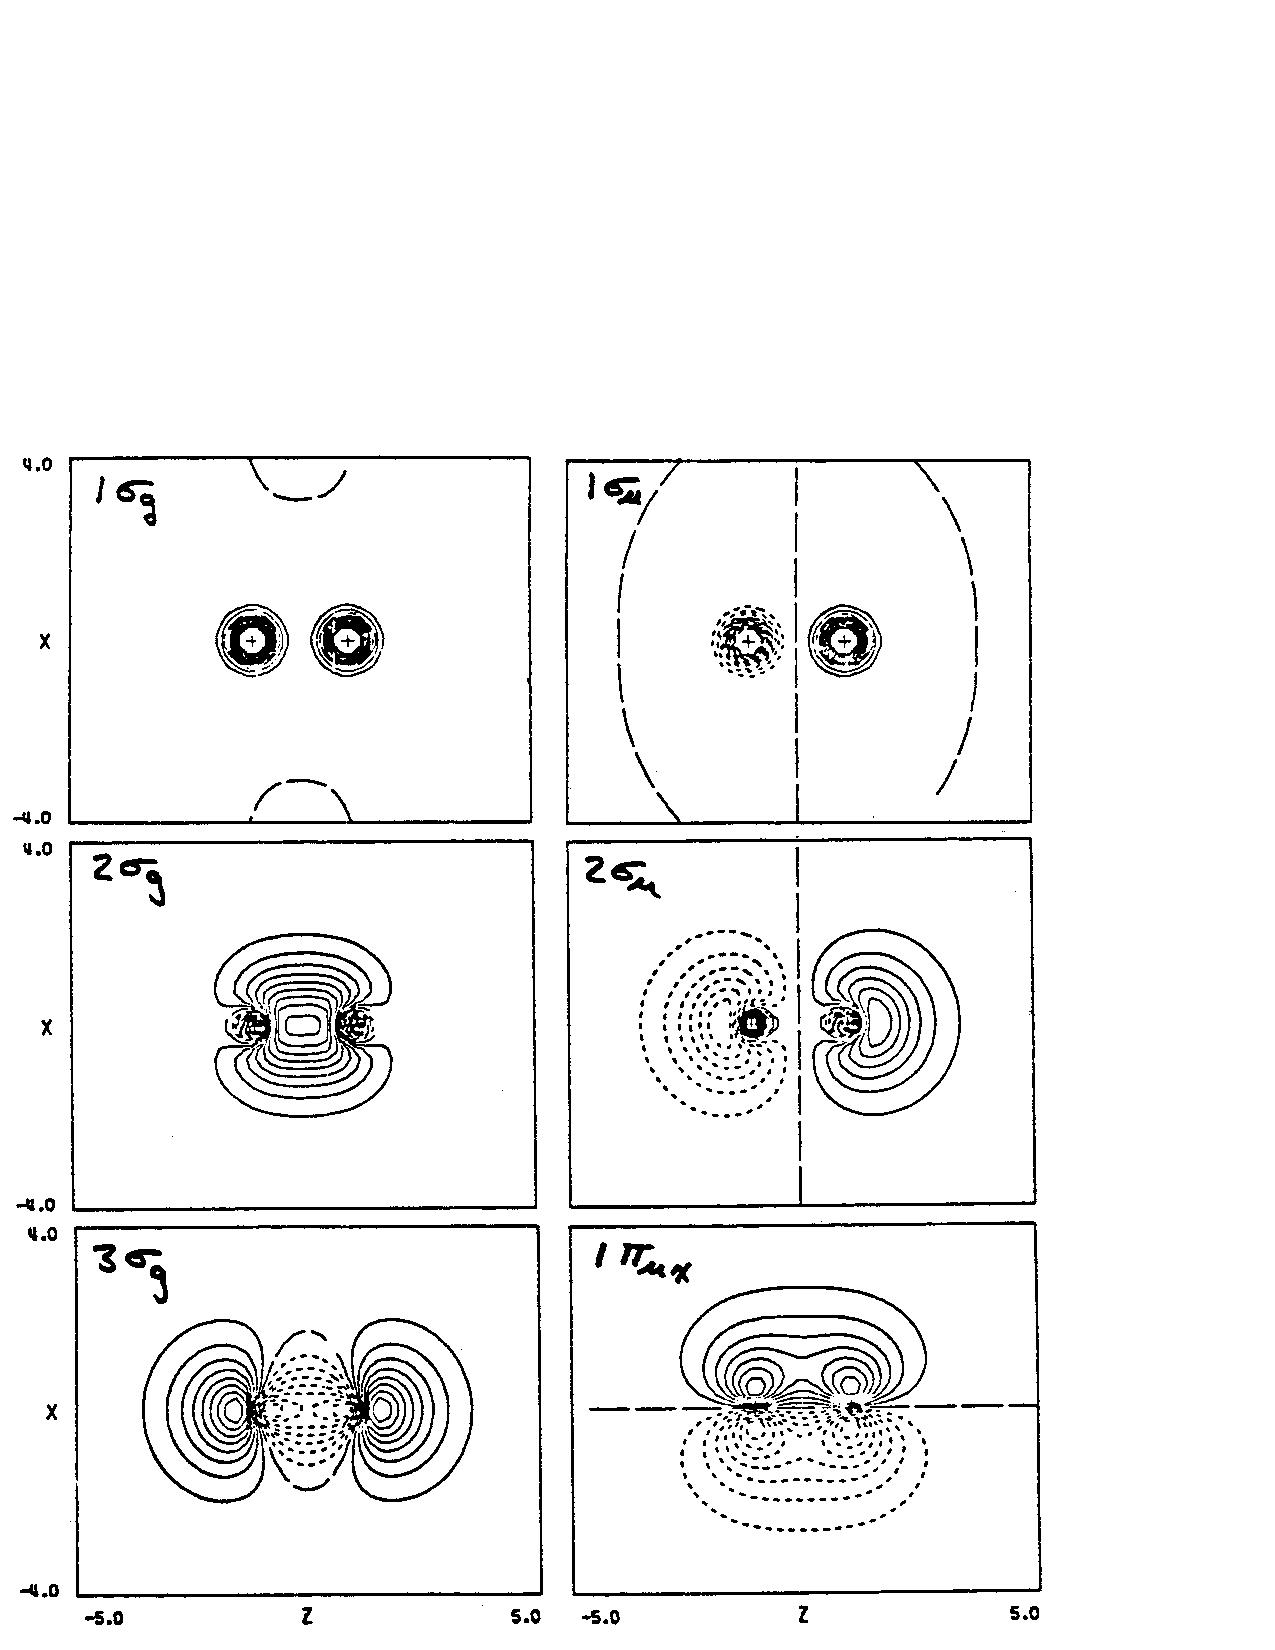
\includegraphics[scale=0.75]{fg10-14}
\caption{HF orbitals for N$_2$, X${^1\Sigma}^+_g$.}
\label{chap10-fig14}
\end{figure}


Schematically, we may indicate the wavefunction in equation
(\ref{chap10-eqno35}) as
\begin{equation}
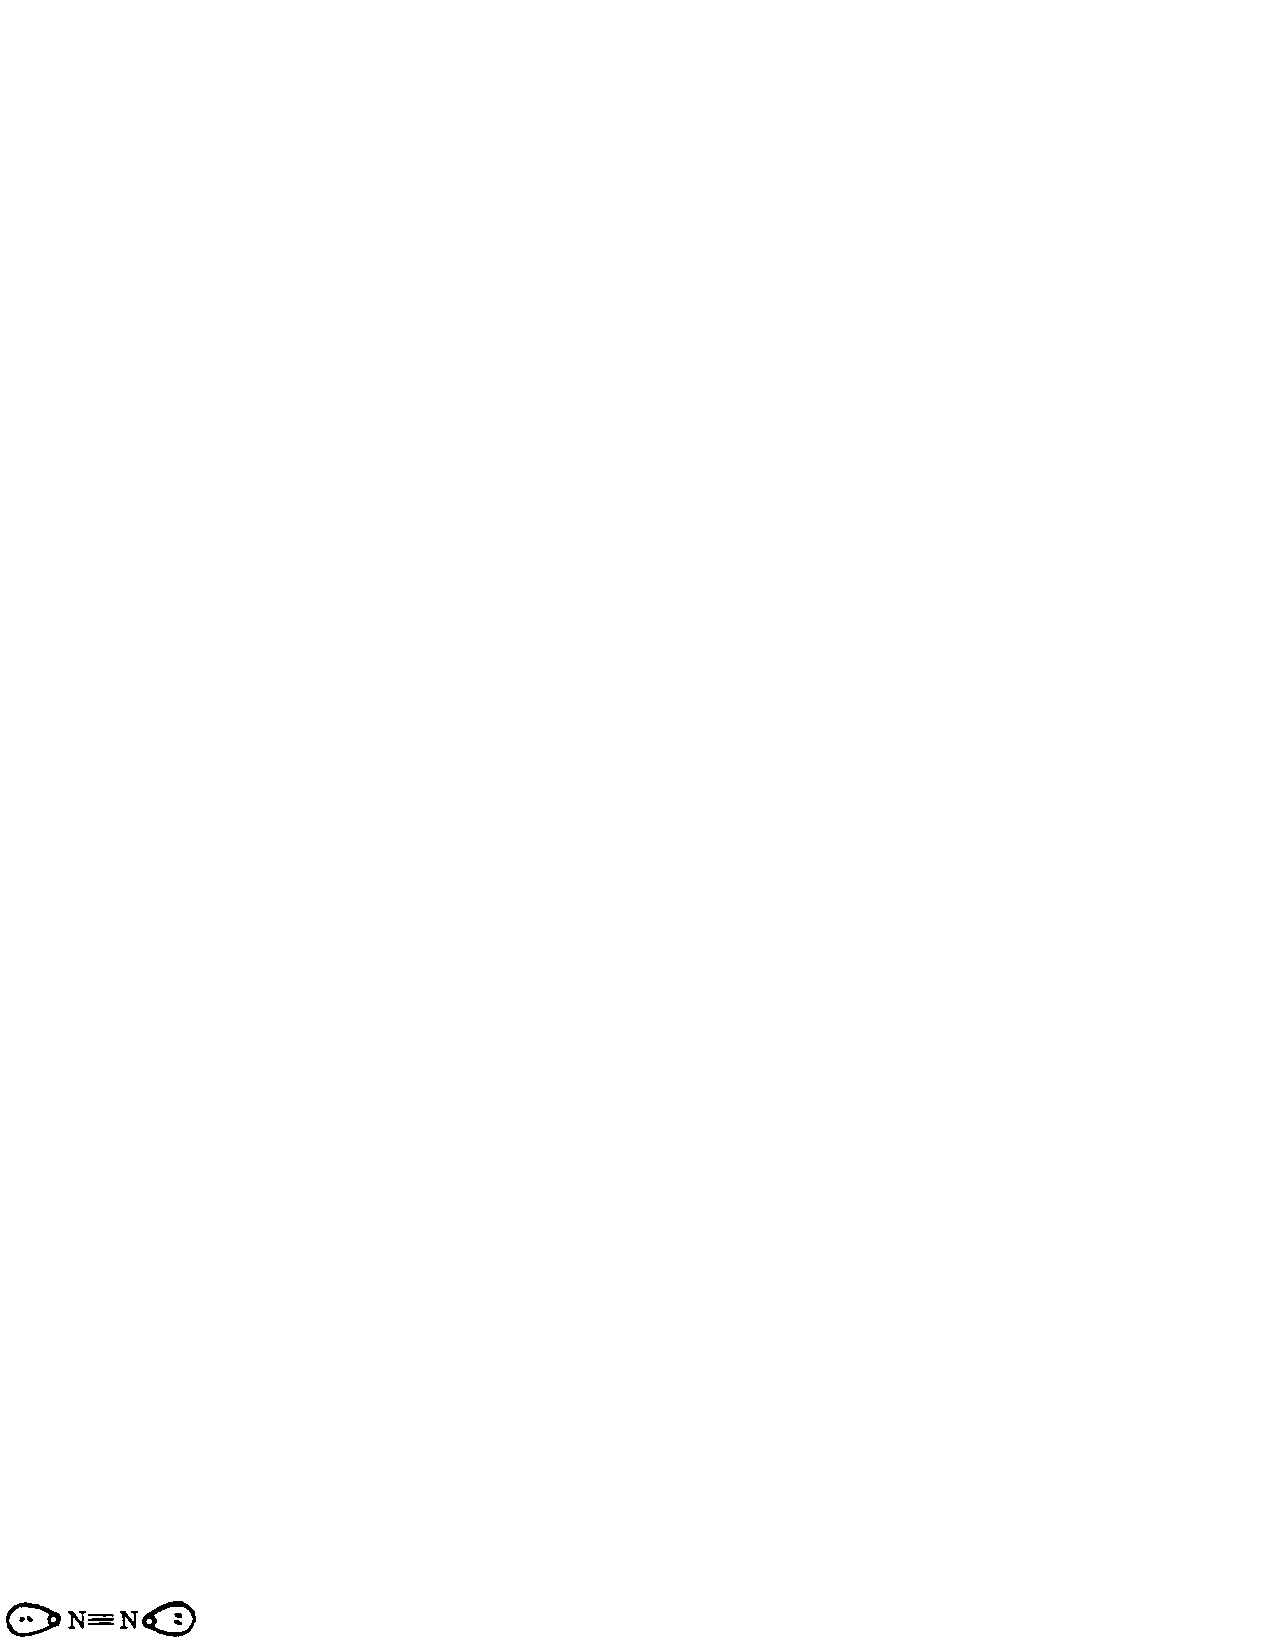
\includegraphics{fg10-12e}
\end{equation}
where each line denotes a two-electron bond.  Considering each bond
pair to be associated with both atoms, we see that each N is
associated with a full octet of electrons.  As indicated in
Table \ref{chap10-tab18}, the bonds of all these species are quite
strong, see also Table \ref{chap10-tab17}.

\begin{table}
\caption{Properties of the N column diatomics.}
\label{chap10-tab18}
\begin{tabular}{cccccccc}\\ \hline

& & $R_e$ & $\omega_e$ &\multicolumn{2}{c}{$D_0$}&
\multicolumn{2}{c}{IP}\cr
& & & & & & Molecule & Atom\cr
& & (\AA) & (cm$^{-1}$) & (eV)& (kcal)&\multicolumn{2}{c}{(eV)}\cr

N$^+_2$ & ${^2\Sigma}^+_g$ & 1.1164 & 2207.0 & 8.712$^8$ & 200.9 & 
27.1\cr
N$_2$ & ${^1\Sigma}^+_g$ & 1.0977 & 2358.6 & 9.759$^4$ & 225.1 & 
15.5808 & 14.53\cr
N$^-_2$ & ${^2\Pi}_g$ & 1.19$^3$ & (1968) & 7.93 & 182.9 & 
$-$1.90$^1$ & $-$0.07\cr
P$^+_2$ & ${^2\Pi}_{ui}$ & 1.985$^9$ & 672.2 & 4.99 & 115.1\cr
P$_2$ & ${^1\Sigma}^+_g$ & 1.8934 & 780.8 & 5.033 & 116.1 & 10.53 & 
10.484\cr
As$_2$ & ${^1\Sigma}^+_g$ & 2.1026 & 429.6 & 3.96 & 91.3 & & 9.81\cr
Sb$_2$ & ${^1\Sigma}^+_g$ & 2.34 & 270.0 & 3.09 & 71.3 & & 8.639\cr
Bi$_2$ & ${^1\Sigma}^+_g$ & 2.6596 & 172.7 & 2.0$^4$ & 47.0	& 7.53 & 
7.287\cr
Pn$^+$ & ${^2\Sigma}^+$ & & [(1200)] & 5.0$^0$ & 115.8\cr
Pn & ${^1\Sigma}^+$ & 1.4909 & 1337.2 & 6.3$^6$ & 146.7 & 11.8$^5$ & 
10.484\cr
AsN & ${^1\Sigma}^+$ & 1.6184 & 1068.5\cr
SbN & ${^1\Sigma}^+$ & & 942.0\cr
AsP & ${^1\Sigma}^+$ & 1.999 & 604.0\cr
SbP & ${^1\Sigma}^+$ & 2.205 & 500.1 & 3.68 & 84.7\cr
SbAs & ${^1\Sigma}^+$ & & 343.0\cr
BiSb & ${^1\Sigma}^+$ & & 220.0\cr
\hline
\end{tabular}
\end{table}

\begin{table}
\caption{Heteronuclear bonds.}
\label{chap10-tab19}
\begin{tabular}{cccccc}\\ \hline

&\multicolumn{2}{c}{Bond Length}&\multicolumn{3}{c}{Bond Energy}\cr
& XY & ${1 \over 2}(X_2+Y_2)$ & XY & ${1 \over 
2}(X_2+Y_2)$&$\sqrt{(X_2)(Y_2)}$\cr
&\multicolumn{2}{c}{(\AA)}&\multicolumn{3}{c}{(kcal)}\cr 

PN & 1.491 & 1.496 & 147 & 170.6 & 161.7\cr
AsN & 1.618 & 1.600\cr
AsP & 1.999 & 1.998\cr
SbP & 2.205 & 2.117 & 84.7 & 93.7 & 91.0\cr
PN$^+$ & - & 1.551 & 115 & 158 & 152.1\cr
\hline
\end{tabular}
\end{table}

The bond strengths and bond distances for the heteronuclear diatomics,
are compared in Table \ref{chap10-tab19}.  Here we see that the bond
distance of XY is close to the average of X$_2$ and Y$_2$, shorter by
0.005 for PN, longer by 0.018, 0.001, and 0.088 for AsN, AsP, and SbP.
The value of 0.088 seems particularly large, perhaps the experiment
for SbP or Sb$_2$ should be reexamined.
	
For the three cases where comparisons can be made, the bond 
energy for the heteronuclear molecule is consistently below 
the average bond energy, contrary to usual expectations.

\subsubsection{Positive Ion States}

Recall the MO configuration for P$_2$
\begin{equation}
\left( \sigma_g 3s \right)^2 \left( \sigma_u 3s 
\right)^2 \left( \sigma_g 3p \right)^2 \left( \pi_u 3p \right)^4
\end{equation}
Since the $\pi$ bond is weaker than the $\sigma$ bond, we would expect
the $\pi_u$ orbital to be easiest to ionize. In fact, this is found
for P$_2 \rightarrow$ P$_2^+$.  However, for N$^+_2$ the ground state
is ${^2\Sigma}^+_g$, that is, ionization is out of the $\sigma_g$ bond
orbital. In order to rationalize the ordering of states for N$^+_2$,
see Table \ref{chap10-tab19}, it is necessary to assume that the
MOs are ordered as
\begin{equation}
\sigma_u 2s < \pi_u 2p < \sigma_g 2p
\end{equation}
or
\begin{equation}
2 \sigma_u < 1 \pi_u < 3 \sigma_g .
\end{equation}
This leads to three low-lying states corresponding to removal 
of the $3\sigma_g$, $1 \pi_u$, or $2 \sigma_u$ orbitals of
\begin{eqnarray}
{^2\Sigma}^+_g &: \left( 2 \sigma_u \right)^2 \left( 1 \pi_u 
\right)^4 \left( 3 \sigma_g \right)^1\cr
{^2\Pi}_u &: \left( 2 \sigma_u \right)^2 \left( 1 \pi_u  s
\right)^3 \left( 3 \sigma_g \right)^2\cr
{^2\Sigma}^+ &: \left( 2 \pi_u p \right)^1 \left( 1 \pi_u 
\right)^4 \left( 3 \sigma_g \right)^2 .
\end{eqnarray}
Since the $3\sigma_g$ and $1 \pi_u$ orbitals are bonding, we expect
the corresponding ion states to have larger bond distances, lower
vibrational frequencies, and weaker bonds. As indicated in Table
\ref{chap10-tab20}, this is observed.  On the other hand, the $2
\sigma_u$ orbital is antibonding, so that removal of the electron from
this orbital leads to a shorter bond and a higher vibrational
frequency.

\begin{table}
\caption{The ground state of N$_2$ and low-lying states of N$^+_2$.}
\label{chap10-tab20}
\begin{tabular}{ccccccc} \\ \hline

& Configuration &\multicolumn{2}{c}{$\Delta E$}&$R_e$ & $\omega_e$ & $D_0$\cr
& & (eV) & (cm${^-1}$) & (\AA) & (cm${^-1}$) & (kcal)\cr

N$_2$ ~ ${^1\Sigma}^+_g$ & (1),(2)& 0 & - & 1.0977 & 2358.027 & 
225.1\cr
N$^+_2$ ~ ${^2\Sigma}^+_g$ & (4),(8) & 15.58 & 0 & 1.116 & 2207.19 & 
(201.3)\cr
~~~~~${^2\Pi}_u$ & (5),(7) & 16.69 & 9016.4 & 1.174 & 1902.84\cr
~~~~~${^2\Sigma}^+_u$ & (1),(8) & 18.76 & 25566.1 & 1.075 & 2419.84\cr
\hline
\end{tabular}
\end{table}

In the GVB model, these ion states have the configurations
\begin{equation}
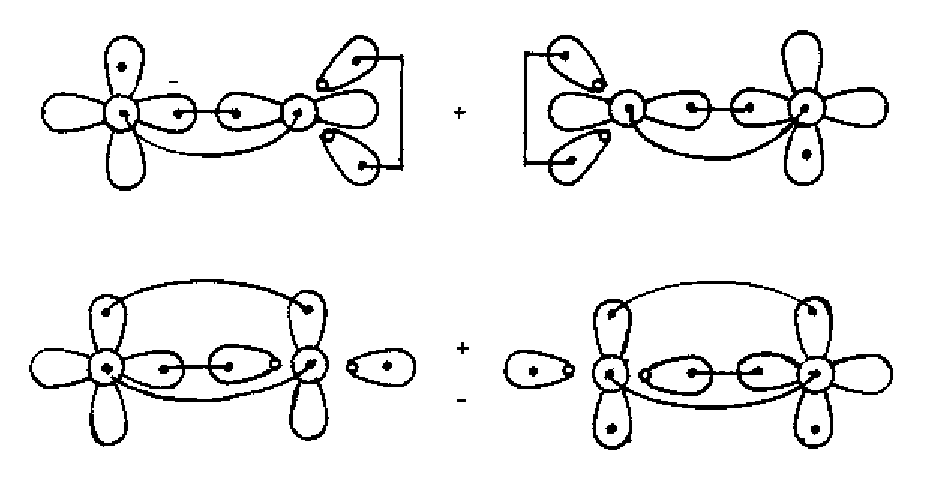
\includegraphics[scale=0.75]{fg10-14a}
\end{equation}
where, in each case, a N atom
\begin{equation}
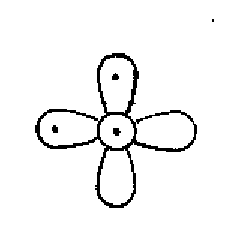
\includegraphics{fg10-14a2}
\end{equation}
($2s$ pair not shown) is bonded to an N$^+$ atom
\begin{equation}
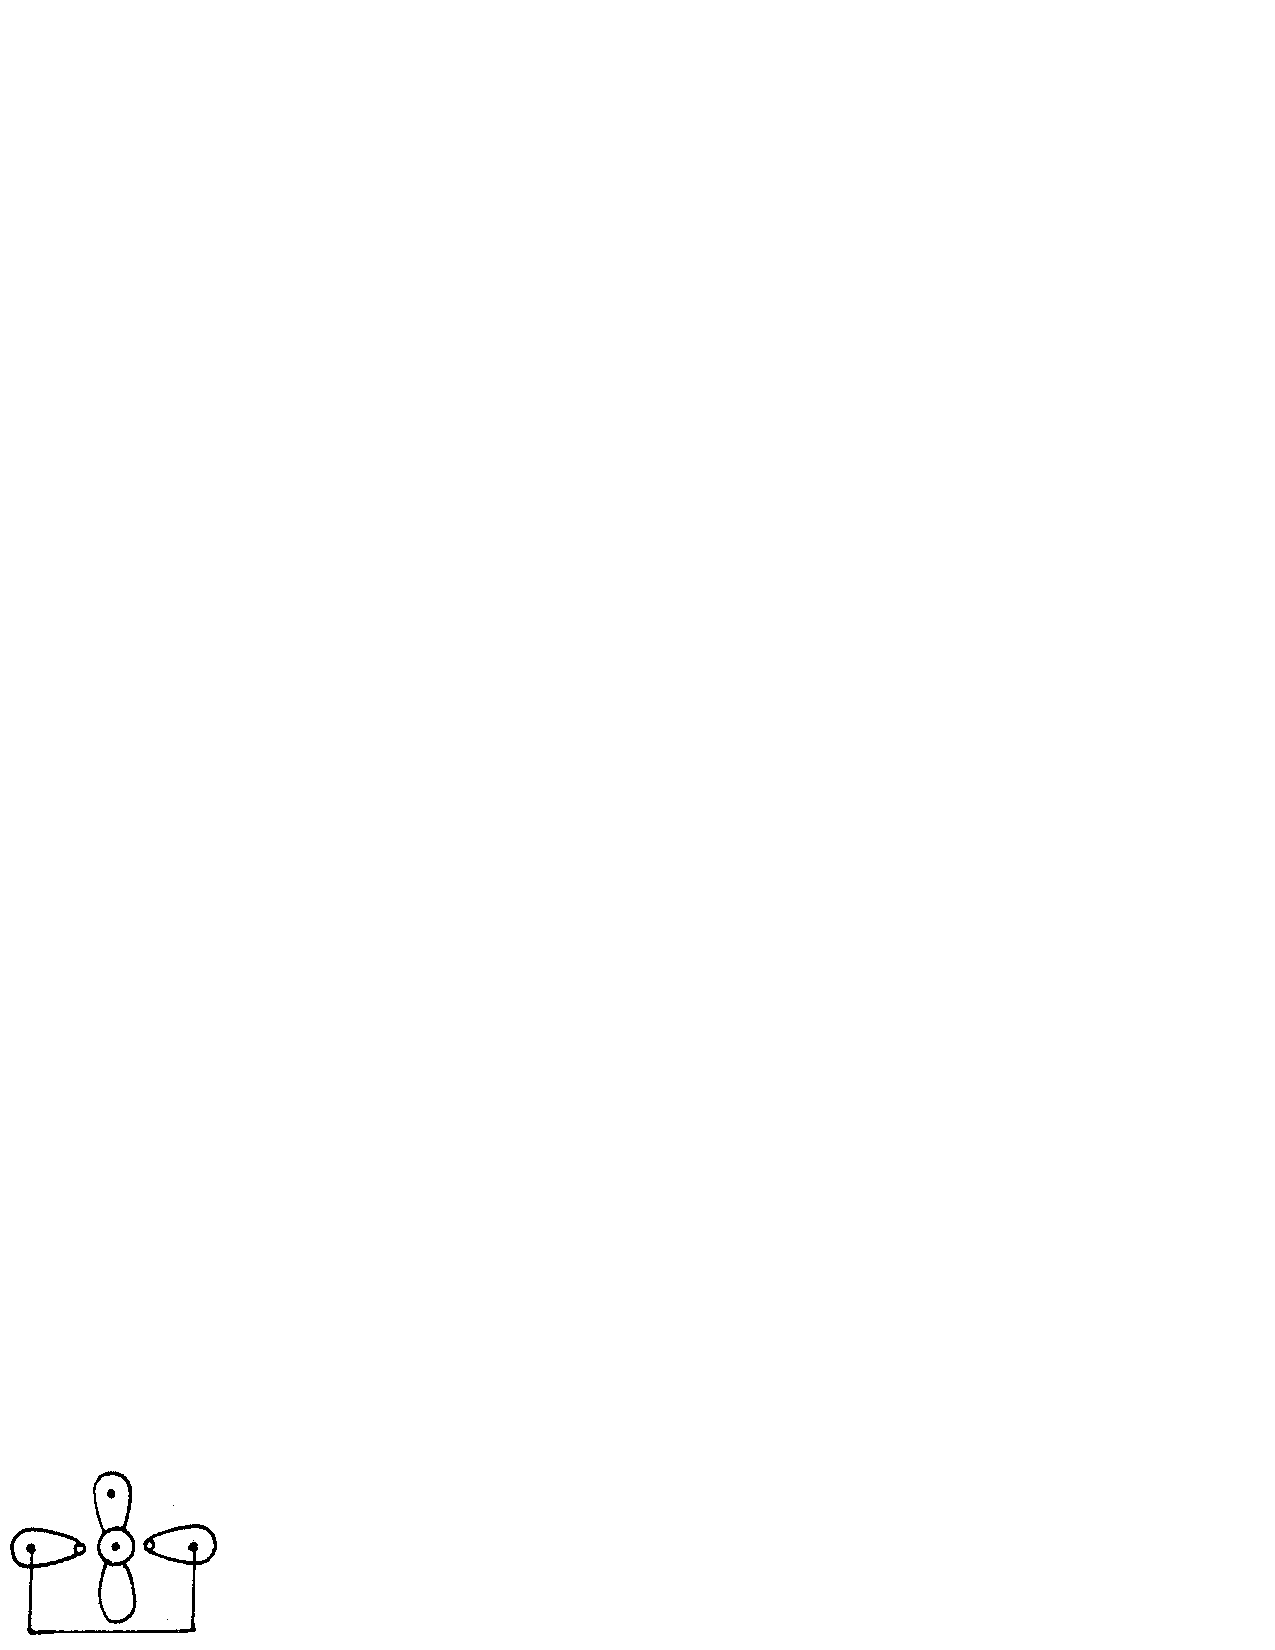
\includegraphics{fg10-14b}
\end{equation}
$2s$ pair correlated into the direction of the missing $p$ orbital. In 
this picture the ${^2\Pi}_u$ state leads to 2-1/2 bonds, but does not involve 
coupling to the $2s$ pair, while the ${^2\Sigma}_g$ 
state leads to three bonds but an unpairing of the $2s$ pair, decreasing the
bond energy.  As found in Chapter 6, unpairing of the $2s$ pair is much more
favorable for $N$ than for P, As, etc., and hence, it is rational that 
${^2\Sigma}_g$  could be the ground state of N$_2^+$.

\subsubsection{Negative Ion States}

\begin{figure}
\begin{center}
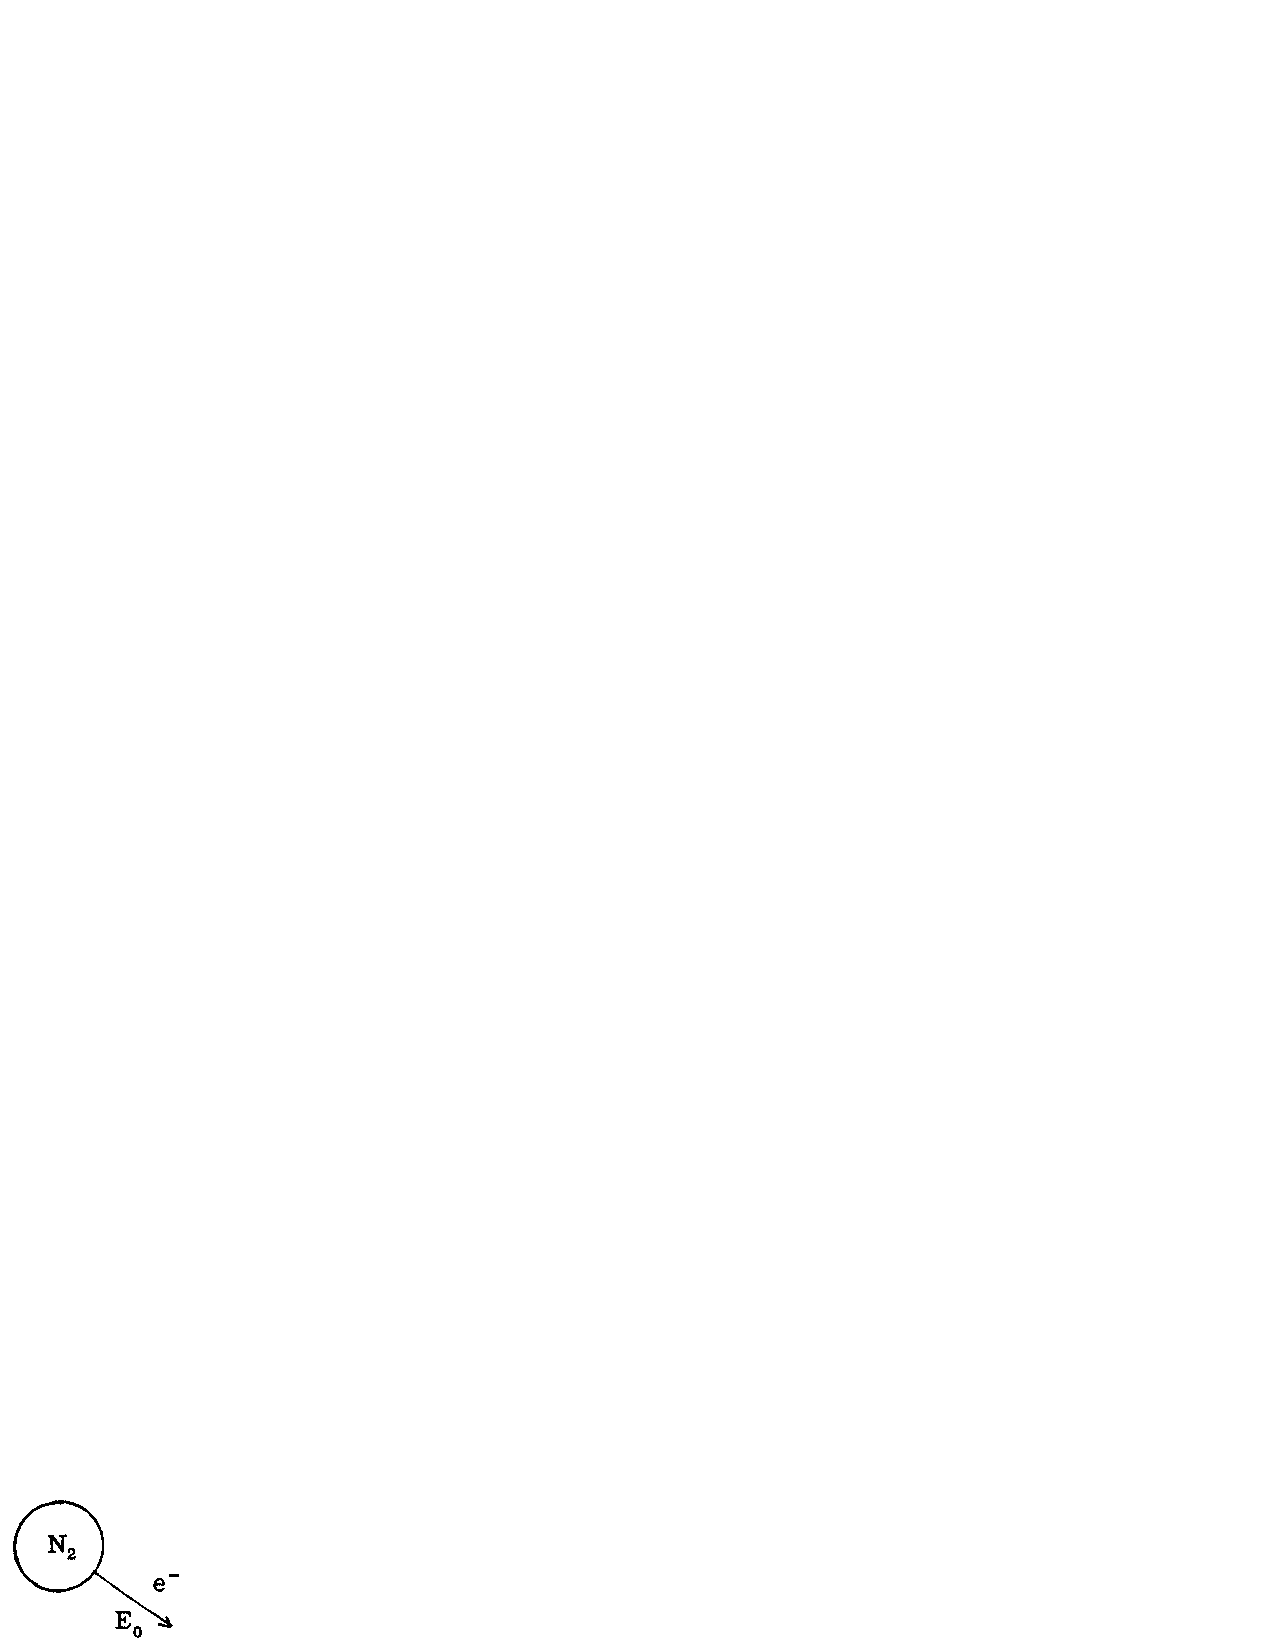
\includegraphics{fg10-15}
\end{center}
\caption{}
\label{chap10-fig15}
\end{figure}

Based on the configuration (\ref{chap10-eqno26}), N$^-_2$ should have
the extra electron in the $( \pi_g 3p)$ orbital, leading to a
${^2\Pi}_g$ state. This is observed, however, the electron affinity,
EA, is $- 1.90$ eV.  That is, N$^-_2$ has an energy 1.9 eV higher than
N$_2$ plus an electron!  The way such a value is measured
experimentally, is to shine a beam of monoenergetic electrons (energy
$E_0$) on gaseous N$_2$ (Figure \ref{chap10-fig15}) and to observe the
elastically scattered electrons as a function of $E_0$. When the
translational energy $E_0$ provides just enough energy to make the
${^2\Pi}_g$ state of N$^-_2$, the electron remains attached to the
N$_2$ for a time long compared to the time for an electron to pass the
N$_2$.  When the electron leaves, it may leave in any direction,
whereas for other values of $E_0$, the electrons scatter forward.  As
a result, the intensity of elastic scattered electrons is a maximum at
$E_0$ (Figure \ref{chap10-fig16}) providing a direct experimental
measure of the negative electron affinity.

\begin{figure}
\begin{center}
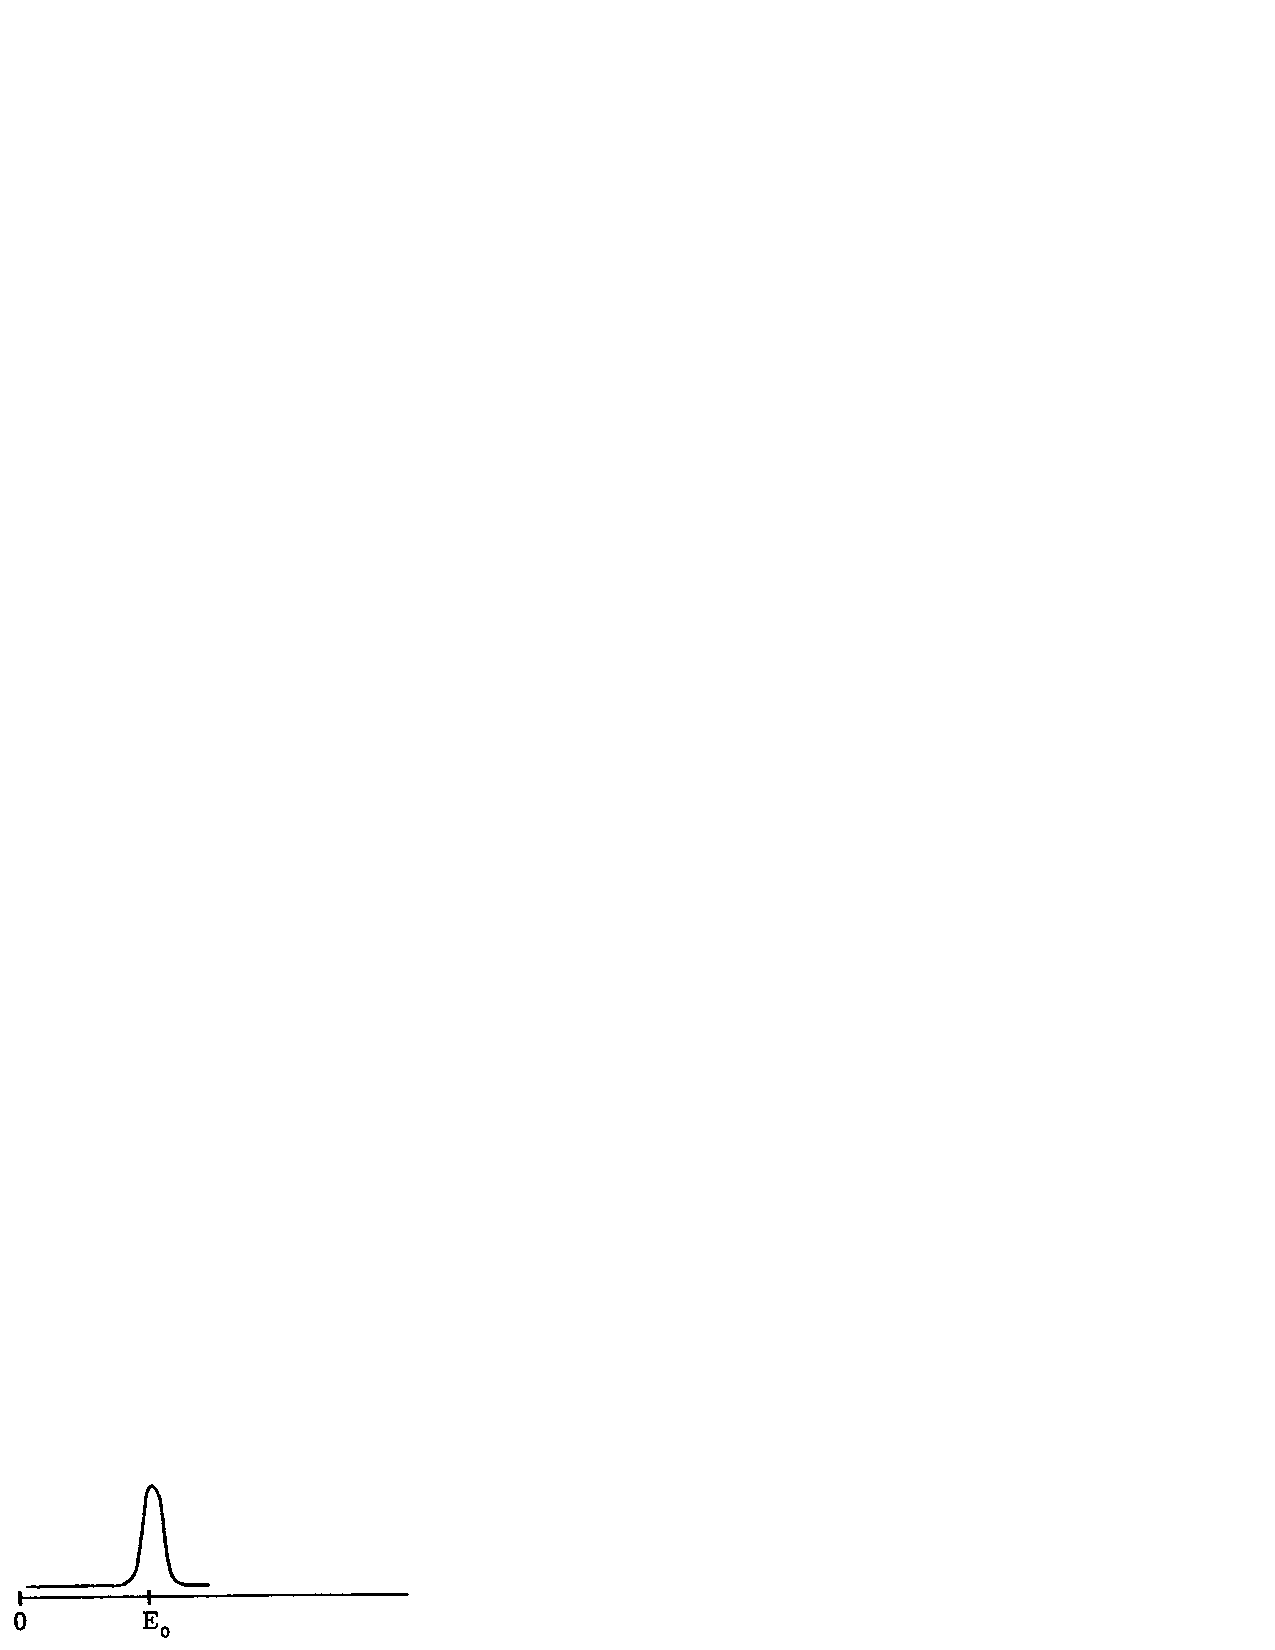
\includegraphics{fg10-16}
\end{center}
\caption{}
\label{chap10-fig16}
\end{figure}

The valence bond diagram for N$^-_2$ is
\begin{equation}
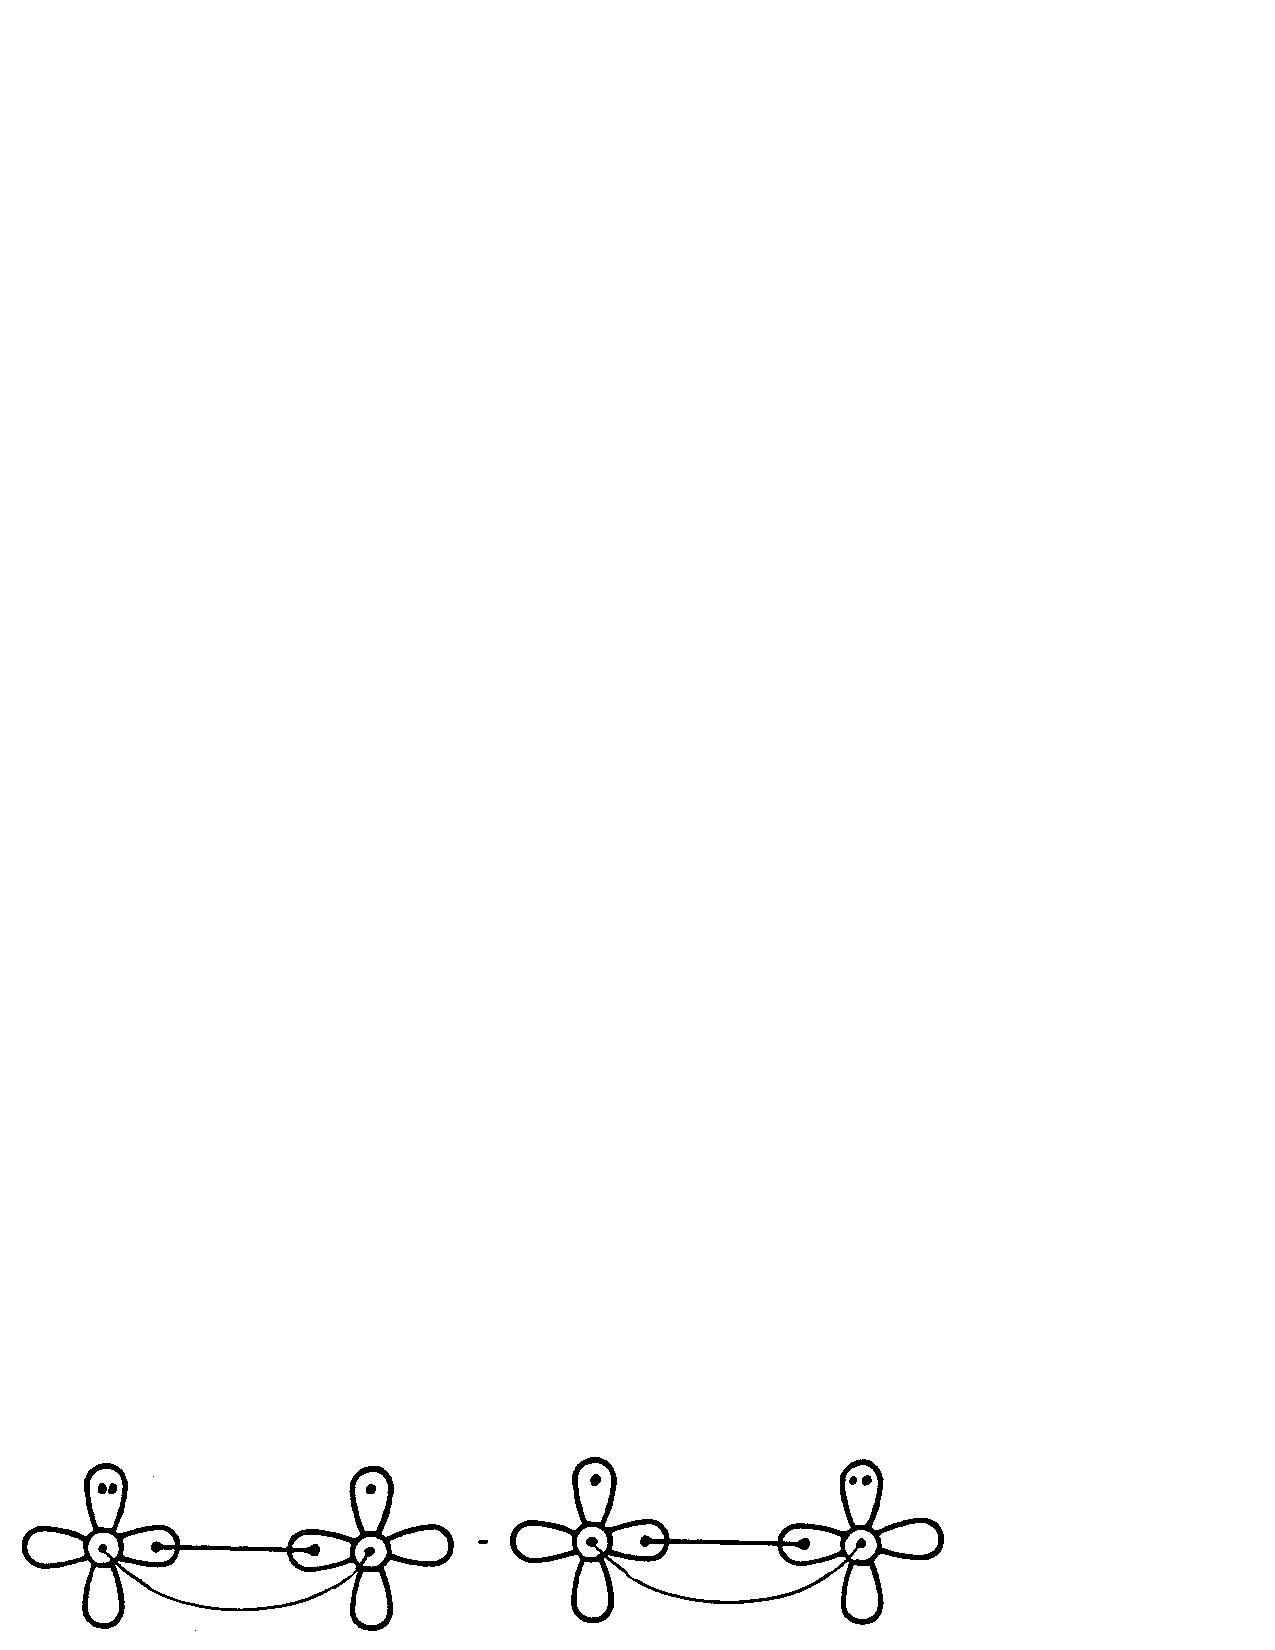
\includegraphics[scale=0.75]{fg10-16a}
\end{equation}
Thus, there are two two-electron bonds and one three-electron bond. From 
the experimental bond energies, one would say that the three-electron 
bond of N$^-_2$ is 42.2 kcal weaker than the two-electron bond of 
N$_2$, while 
the one-electron bond of N$^+_2$ is 24.2 kcal weaker than the two-electron 
bond of N$_2$.  Such comparisons 
are somewhat ambiguous, since the bond lengths change and since a change in
occupation of one orbital does affect the other orbitals.

\subsection{The O Column}

\subsubsection{Neutrals}

The elements O, S, Se, Te, and Po, all have a $(ns)^2 (np)^4$ valence
configuration, leading to a ${^3\Sigma}^-_g$ ground state, from
equation (\ref{chap10-eqno26}), for the homonuclear diatomics
\begin{equation}
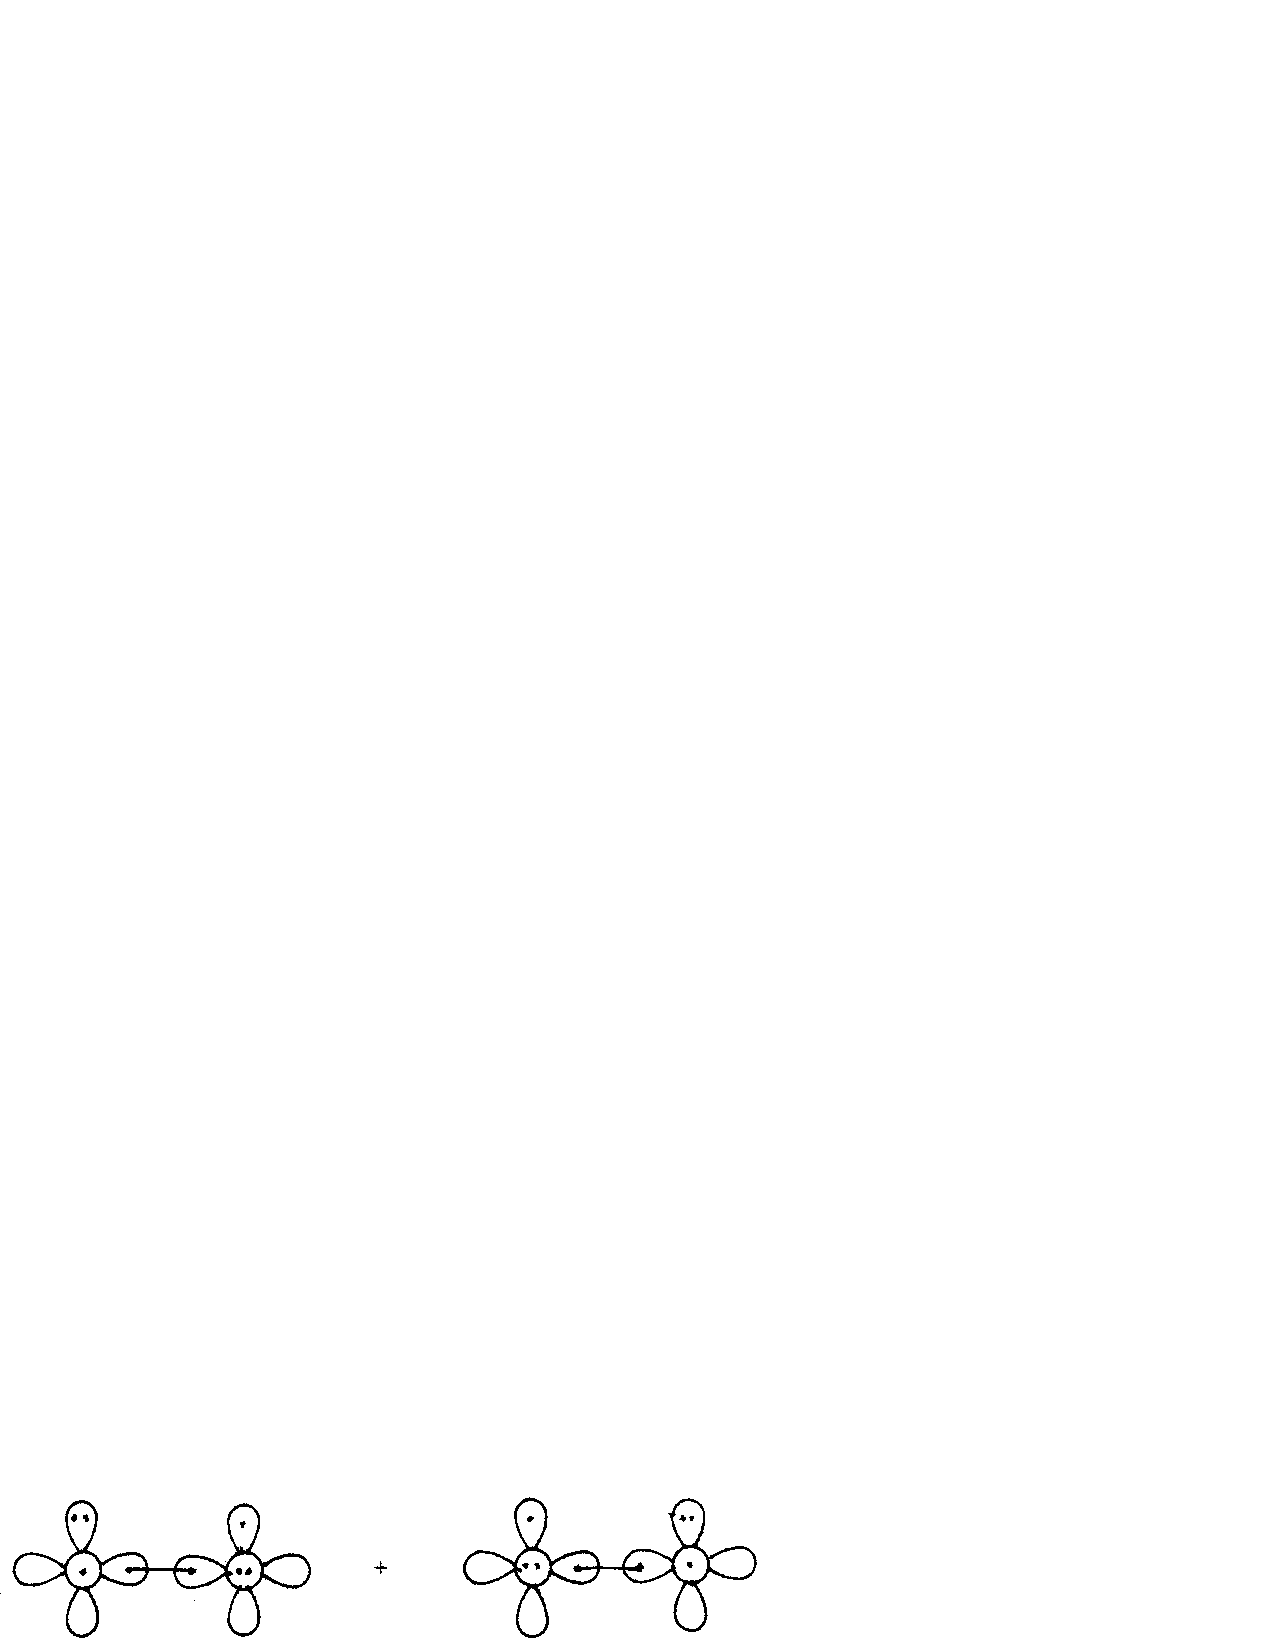
\includegraphics{fg10-16b}
\label{chap10-eqno36}
\end{equation}
or
\begin{equation}
\left( \sigma_g ns \right)^2 \left( \sigma_u ns 
\right)^2 \left( \sigma_g np \right)^2 \left( \pi_u np \right)^4
\left( \pi_g np \right)^2
\end{equation}
The bonds are quite strong, as indicated in Table \ref{chap10-tab21}
(more complete results are in Table \ref{chap10-tab22}).  Just as for
other columns, the bond strengths decrease, the bond lengths increase,
and the vibrational frequencies decrease as we proceed down the
column.

\begin{figure}
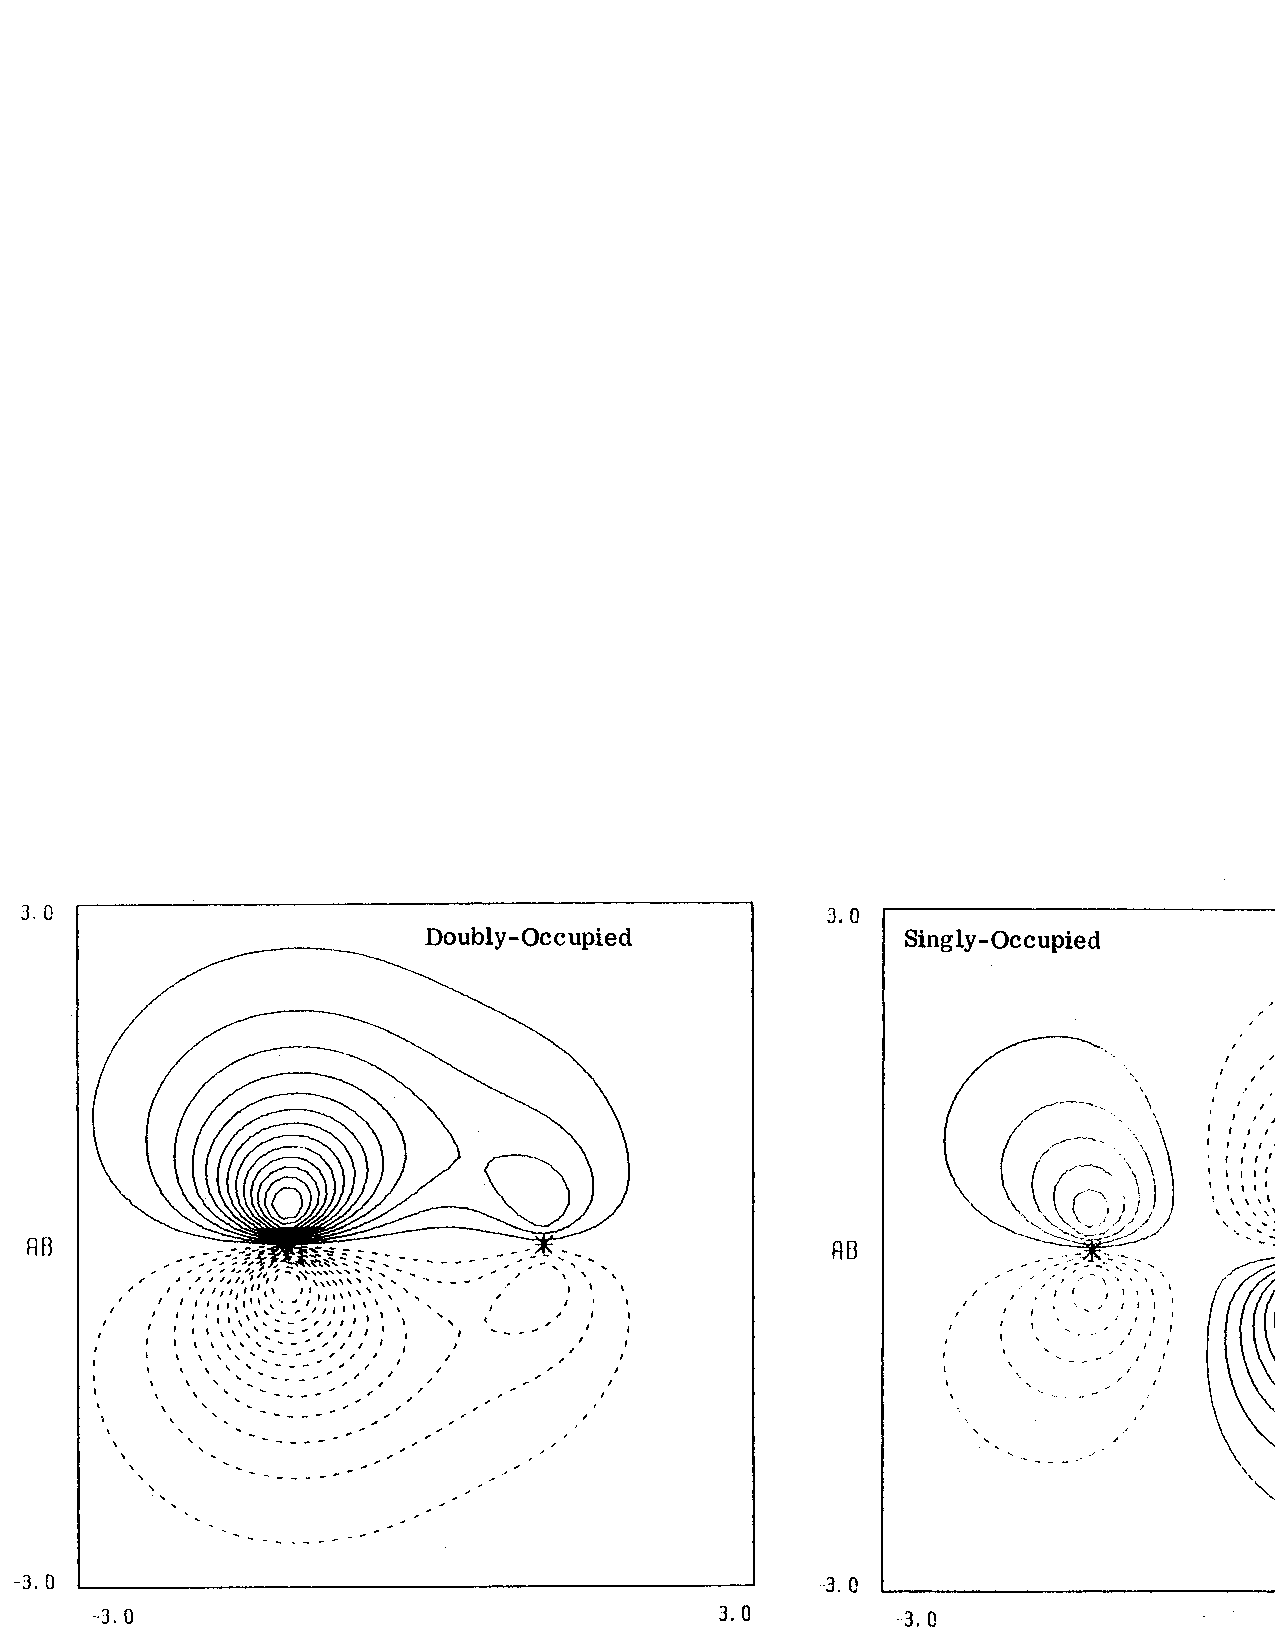
\includegraphics[scale=0.75,angle=90]{fg10-17}
\caption{The optimum $\pi_y$ orbitals from configuration
\ref{chap10-eqno36}.} 
\label{chap10-fig17}
\end{figure}

\begin{figure}
\includegraphics[scale=0.75]{fg10-18}
\caption{The GVB orbitals of O$_2$.}
\label{chap10-fig18}
\end{figure}

\begin{table}
\caption{}
\label{chap10-tab21}
\begin{tabular}{cccc}\\ \hline

& $R_e$ & $\omega_e$ & $D_0$\cr
& (\AA) & (cm${^-1}$) & (kcal)\cr

O$_2$ & 1.208 & 1580 & 118.0\cr
S$_2$ & 1.889 & 726 & 100.8\cr
Se$_2$ & 2.166 & 385 & 78.7\cr
Te$_2$ & 2.557 & 247 & 61.7\cr
Po$_2$ & & 156 & 44\cr
\hline
\end{tabular}
\end{table}


\begin{table}
\caption{}
\label{chap10-tab22}
\begin{tabular}{cccccccc}\\ \hline

& Symmetry$^a$ & $R_e$ & $\omega_e$ &\multicolumn{2}{c}{$D_0$}
&\multicolumn{2}{c}{IP (eV)}\cr
& & (\AA)& (cm${^-1}$)& (eV) & (kcal)& Molecule & Atom\cr
O$^+_2$ & ${^2\Pi}_g$ & 1.1164 & 1904.8	 & 6.663 & 153.65 & 24.2\cr
O$_2$ & ${^3\Sigma}^-_g$ & 1.2075 & 1580.2 & 5.115$^6$ & 117.97 & 
12.071 & 13.614\cr
O$^-_2$ & ${^2\Pi}_{gi}$ & 1.35 & 1090 & 4.09$^4$ & 94.41 & 0.440 & 
1.462\cr
S$^+_2$ & ${^2\Pi}_{gr}$ & (1.82$^5$) & 790 & 5.37 & 123.8\cr
S$_2$ & ${^3\Sigma}_g$ & 1.8892 & 725.7 & 4.3693 & 100.76 & 9.36 & 
10.357\cr
S$^-_2$ & ${^2\Pi}_{gi}$ & & 600.8 & 3.95$^5$ & 91.20 & 1.66$^3$ & 
2.0772\cr
Se$^+_2$ & ${^2\Pi}_{gr}$ & & & 4.2$^8$ & 98.7\cr
Se$_2$ & ${^3\Sigma}^-_g$ &2.166$^0$ & 385.3 & [3.411]$^b$ & 
78.66$^b$ & 8.88 & 9.75\cr
Se$_2$ & & & 330.$^3$ & & & & 2.0206\cr
Te$^+_2$ & $({^2\Pi}_{gr})$ & & & 3.40 & 78.4\cr
Te$_2$ & ${^3\Sigma}^-_g$ & 2.5574 & 247.1 & 2.677 & 61.73 & 8.29 & 
9.01\cr
Po$_2$ & & & 155.7 & (1.90) & 43.8 & & 8.43\cr
SO$^+$ & ${^2\Pi}_r$ & (1.42$^4$) & 1360 & 5.43 & 125.2\cr
SO & ${^3\Sigma}^-$ & 1.4811 & 1149.2 & 5.359 & 123.58 & 10.29 & 
10.357\cr
SeO & ${^3\Sigma}^-$ & 1.648$^4$ & 914.7 & $\leq 4.4^1$ & 
$\leq$101.7\cr
TeO$^+$ & ${^2\Pi}_r$ & & & $\leq$4.19 & $\leq$96.6\cr
TeO & $0^+$ & 1.825$^0$ & 797.1 & $\leq$3.90 & $\leq$89.9 & 8.72 & 
9.01\cr
SeS & ${^3\Sigma}^-$ & 2.036$^7$ & 555.6 & (3.7) & 85.3\cr
SeS$^-$ & $({^2\Pi})$ & & 468.9 & $<3.3$ & $<76.1$\cr
TeS & $0^+$ & 2.2297 & 471.2 & (3.5) & 80.7\cr
TeSe & $0^+$ & (2.37$^2$) & 316.2 & 3.0 & 69.2\cr
\hline
\end{tabular}\\
$^a$ 0$^+$ is the lone energy component of a ${^3\Sigma}^-$ state for 
which there is a large amount of spin-orbit coupling.
$^b$ Reference 2 suggests $D_0 =$ 73. 0 kcal.
\end{table}

For O$_2$ the MO configuration, from Table
\ref{chap10-tab35}, is
\begin{equation}
\underbrace{(1 \sigma_g)^2 (1 \sigma_u)^2}_{O1s}
\underbrace{(2 \sigma_g)^2 (2 \sigma_u)^2}_{O2s} 
\underbrace{(3 \sigma_g)^2 (1 \pi_u)^4}_{bonding}
\underbrace{(1 \pi_g)^2}_{antibonding}
\end{equation}
As compared with N$_2$, there are now six electrons in bonding 
orbitals and two in antibonding orbitals, leading to a much weaker
bond.

With two electrons in the $\pi_g$ orbitals, we can form four possible 
two-electron wavefunctions. Combining with spin functions and 
taking care of Pauli and Hund, leads to a ground state of the form
\begin{equation}
\left( \pi_{gz} \pi_{gy} - \pi_{gy} \pi_{gx} \right) ( \alpha \alpha )
\end{equation}
of ${^3\Sigma}^-_g$ symmetry. The singlet wavefunctions lead to 
${^1\Delta}_g$ and ${^1\Sigma}^+_g$ states in Figure \ref{chap10-fig3}.

Sometimes the bonding in O$_2$ is drawn as
\begin{equation}
\includegraphics{fg10-18a}
\end{equation}
Although this properly indicates the net double bond, it does not 
properly indicate the triplet character of the wavefunction. Since 
there are two electrons in each of the two bonding orbitals, and 
one in each of the two antibonding orbitals, we consider these 
to be two three-electron bonds,
\begin{equation}
\includegraphics{fg10-18b}
\end{equation}
The $\pi_y$ orbitals for O$_2$ are shown in Figure \ref{chap10-fig17},
and the $\sigma$ orbitals are shown in Figure \ref{chap10-fig18}.
These $\pi$ orbitals were obtained from calculations in which the
orbitals were optimized for the configuration shown in equation
(\ref{chap10-eqno36}).

\begin{table}
\caption{Heteronuclear bonds.}
\label{chap10-tab23}
\begin{tabular}{ccccc}\\ \hline

&\multicolumn{2}{c}{Bond Distance (\AA)}&\multicolumn{2}{c}
{Bond Energy (kcal)}\cr
& $XY$ & ${1 \over 2}(X_2+Y_2)$ & $XY$ & ${1 \over 2}(X_2+Y_2)$\cr

SO$^+$ & (1.42$^4$) & (1.47$^1$) & 125.2 & 120.9$^a$\cr
SO & 1.481 & 1.548 & 123.6 & 109.4\cr
SeO & 1.648 & 1.687 & $\leq$101.7 & 98.3\cr
TeO$^+$ & & & $\leq$96.6 & 98.2$^a$\cr
TeO & 1.825 & 1.883 & $\leq$89.9 & 89.9\cr
SeS & 2.037 & 2.028 & 85.3 & 78.2\cr
SeS$^-$ & & & $\leq$76.4 & 84.9$^b$\cr
TeS & 2.230 & 2.223 & 80.7 & 81.2\cr
TeSe & (2.37$^2$) & 2.362 & 69.2 & 70.2\cr
\hline
\end{tabular}\\
$^a$ Based on ${1 \over 2}(X^+_2 +O_2)$.  Using ${1 \over 2}(X_2 + 
O^+_2)$ would have given 138.7 as the average for SO$^+$ and 116.0 for 
TeO$^+$.
$^b$ Based on ${1 \over 2}(Se_2 + S^-_2)$.
\end{table}

Properties of the heteronuclear bonds are compared in Table
\ref{chap10-tab23}.  For the oxides, the bond length of XO is
generally shorter than the average ${1 \over 2}( X_2 + O_2)$
by approximately 0.05 \AA.  On the other hand, for the non-oxides 
the bond length of XY is greater than ${1 \over 2}(X_2+Y_2)$
by approximately 0.01\AA.

Considering neutral molecules, the bond energy of SO is considerably
(14 kcal) stronger than the average ${1 \over 2}(S_2+O_2)$.  However,
for other oxides and non-oxides, the bond energy of XY is close to the
average.  For the positive ions, SO$^+$ and TeO$^+$, the bond energy
of XO$^+$ is considerably smaller than the average of ${1 \over 2}(X_2
+ O^+_2)$ whereas the bond energy of XO$^+$ is close to the average
${1 \over 2}(X^+_2 + O_2)$.  This is reasonable since the ionization
potential of XO$^+$ corresponds to the value of X rather than O.

\subsubsection{Ion States}

\begin{table}
\caption{Bond energy changes, in kcal.}
\label{chap10-tab24}
\begin{tabular}{cccccc} \\ \hline

& & & $\mathrm{IP}_{mole}-\mathrm{IP}_{atom}$ & $EA_{mole}-EA_{ion}$\cr
& & & (eV) & (eV)\cr
& X$^+_2$ to X$_2$ & X$_2$ to X$^-_2$ & X$_2$ & X$_2$\cr

O & $-$35.7 & $-$23.6 & $-$1.54 & $-$1.022\cr
S & $-$23.1 & $-$9.5 & $-$1.00 & $-$0.414\cr
Se & $-$22.4 & & $-$0.87\cr
Te & $-$16.7 & & $-$0.72\cr
\hline
\end{tabular}
\end{table}

\begin{table}
\caption{}
\label{chap10-tab25}
\begin{tabular}{cccccc} \\ \hline

& State & Configuraton & $R_e$ & $\omega_e$ & $D_0$\cr
& & & (\AA) & (cm$^{-1}$) & (kcal)\cr

O$^+_2$ & ${^2\Pi}_{gr}$ & $(1 \pi_g)^1$ & 1.116 & 1905 & 154\cr
O$_2$ & ${^3\Sigma}^-_g$ & $(1 \pi_g)^2$ & 1.208 & 1580 & 118\cr
O$^-_2$ & ${^1\Pi}_{gi}$ & $(1 \pi_g)^3$ & 1.35 & 1090 & 94\cr
\hline
\end{tabular}
\end{table}

Since the $1 \pi_g$ orbital is antibonding, then removing an electron
to form O$^+_2$, leads to a stronger, shorter bond.  While adding a
third electron to the $\pi_g$ orbitals leads to a weaker, longer bond,
as indicated in Table \ref{chap10-tab25}.

The changes in bond energy suggest that the $\pi_g$ orbital is significantly
more antibonding for O$_2$ than for the other molecules.  Equivalently, 
the ionization potential and electron affinity of O$_2$ 
are both decreased from the atomic values by an extra 0.6 eV,
more than the decrease for S$_2$.

\subsection{The F Column}

The elements F, Cl, Br, and I all have an $(ns)^2 (np)^2$ valence 
configuration, leading to a ${^1\Sigma}_g$ ground state with valence 
bond configuration
\begin{equation}
\includegraphics{fg10-18c}
\end{equation}
and MO configuration
\begin{equation}
(\sigma_g 3s)^2 (\sigma_u 3s)^2
\underbrace{(\sigma_g 3p)^2 (\pi_u 3p)^4}_{bonding}
\underbrace{(\pi_g 3p)^4}_{antibonding} .
\end{equation}
Adding in the $ns$ orbitals, leads to
\begin{equation}
\includegraphics{fg10-18d}
\end{equation}
where the F $2s$ lone pairs are also shown, and we see that each F
has an octet of valence electrons.

\begin{table}
\caption{}
\label{chap10-tab26}
\begin{tabular}{cccc} \\ \hline

& $R_e$ & $\omega_e$ & $D_0$\cr
& (\AA) & ( cm$^{-1}$) & (kcal)\cr

F$^+_2$ & 1.412 & 917 & 36.8\cr
Cl$_2$ & 1.988 & 560 & 57.2\cr
Br$^-_2$ & 2.281 & 325 & 45.4\cr
I$_2$ & 2.66 & 215 & 35.6\cr
\hline
\end{tabular}
\end{table}

\begin{table}
\caption{}
\label{chap10-tab27}
\begin{tabular}{cccccccc} \\ \hline

& Symmetry & $R_e$ & $\omega_e$ &\multicolumn{2}{c}{$D_0$}
&\multicolumn{2}{c}{IP (eV)}\cr
& & (\AA)& (cm${^-1}$) & (eV) & (kcal)& Molecule & Atom\cr
F$^+_2$ & ${^2\Pi}_{gi}$ & 1.322 & 1073.3 & 3.33$^9$ & 77.0\cr
F$_2$ & ${^2\Sigma}^+_g$ & 1.4119 & 916.6 & 1.602 & 36.9 & 15.686 & 
17.418\cr
F$^-_2$ & ${^2\Sigma}^+_u$ & (1.8$^8$) & (510) & 1.28 & 29.5 & 3.08 & 
3.39$^9$\cr
Cl$^+_2$ & ${^1\Sigma}^+_{gi}$ & 1.8915 & 645.6 & 3.95 & 91.1\cr  
Cl$_2$ & ${^1\Sigma}^+_g$ & 1. 987$^9$ & 559.7 & 2.4794 & 57.2 & 
11.50 & 13.01\cr
Cl$^-_2$ & (${^2\Sigma}^+_u$) & & & 1.26 & 29.1 & 2.39 & 
3.61$^5$\cr 
Br$^+_2$ & ${^2\Pi}_g$ & & 376.0 & 3.26 & 75.2\cr
Br$_2$ & ${^1\Sigma}^+_g$ & 2.2811 & 325.3 & 1.9707 & 45.4 & 10.52 & 
11.84\cr
Br$^-_2$ & (${^2\Sigma}^+_u$) & & & 1.15 & 26.5 & 2.55 & 
3.36$^4$\cr 
I$^+_2$ & ${^2\Pi}_{gi}$ & & 240 & (2.683) & 61.9\cr
I$_2$ & ${^1\Sigma}^+_g$ & 2.66$^3$ & 214.5 & 1.5424 & 35.6 & 
(9.311) & 10.454\cr
I$^-_2$ & (${^2\Sigma}^+_u$) & & & 1.04 & 24.0 & 2.56 & 
3.06$^1$\cr 
ClF$^+$ & ${^2\Pi}_i$ & & (870) & 2.93 & 67.6\cr
ClF & ${^1\Sigma}^+$ & 1.6283 & 786.2 & 2.617$^3$ & 60.4 & 12.66 & 
13.01\cr
BrF$^+$ & ${^2\Pi}_i$ & & & 2.61 & 60.2\cr
BrF & ${^1\Sigma}^+$ & 1.7589 & 670.8 & 2.54$^8$ & 58.8 & 11.78 & 
11.84\cr
IF & ${^1\Sigma}^+$ & 1.9098 & 610.2 & 2.87$^9$ & 66.4 & (10.5) & 
10.454\cr
BrCl & ${^1\Sigma}^+$ & 2.1361 & 444.3 & 2.23$^3$ & 51.5 & 11.1 & 
11.84\cr
ICl$^+$ & ${^2\Pi}_i$ & & & 2.52 & 58.1\cr
ICl & ${^1\Sigma}^+$ & 2.3209 & 384.3 & 2.1531 & 49.7 & 10.08 & 
10.454\cr
IBr$^+$ & ${^2\Pi}_i$ & & & 2.42 & 55.8\cr
IBr & ${^1\Sigma}^+$ & 2.4690 & 268.6 & 1.817$^6$ & 41.9 & 9.85 & 
10.454\cr 
IBr$^-$ & & & & 1.1$^2$ & 25.8 & 2.6$^7$ & 3.36$^4$\cr
\hline
\end{tabular}
\end{table}


Comparisons of some properties are given in Tables \ref{chap10-tab26}
and \ref{chap10-tab27}.  Bond length increases by 0.58 \AA\ for F$_2$
to Cl$_2$, by 0.29 \AA\ for Cl$_2$ to Br$_2$, and by 0.39 \AA\ for
Br$_2$ to I$_2$.  The smaller decrease from Cl$_2$ to Br$_2$ is due to
the presence of a $(3d)^{10}$ core for Br and a $(4d)^{10}$ core for
I, permitting slightly greater penetration of the valence electrons.
We find a gradually increasing bond energy for I$_2$ to Br$_2$ to
Cl$_2$, but a very weak bond for F$_2$.  The reason for this is that
the $\pi$ pairs on adjacent F have much higher overlaps than for Cl,
leading to much larger repulsive forces.  This effect also explains
the strange fact that the bond for O-O is very weak compared to
analogous molecules with S-S, SeSe, and Te-Te single bonds, despite
the fact that of the diatomics O$_2$ has, by far, the strongest bond,
see Chapter 9 for a discussion.

\begin{table}
\caption{}
\label{chap10-tab28}
\begin{tabular}{ccccc} \\ \hline

&\multicolumn{2}{c}{$R_e$ (\AA)}&\multicolumn{2}{c}{$D_0$ (kcal)}\cr
& $XY$ & ${1 \over 2}(X_2+Y_2)$ & $XY$ & ${1 \over 2}(X_2+Y_2)$\cr
ClF$^+$ & & & 67.6 & 64.0$^a$\cr
ClF & 1.628 & 1.700 & 60.4 & 47.1\cr
BrF$^+$ & & & 60.2 & 56.1$^a$\cr
BrF & 1.759 & 1.847 & 58.8 & 41.2\cr
IF & 1.910 & 2.039 & 66.4 & 36.3\cr
BrCl & 2.136 & 2.135 & 51.5 & 51.3\cr
ICl$^+$ & & & 58.1 & 59.6$^b$\cr
ICl & 2.321 & 2.327 & 49.7 & 46.4\cr
IBr$^+$ & & & 55.8 & 53.7$^b$\cr
IBr & 2.469 & 2.474 & 41.9 & 40.5\cr
IBr$^-$ & & & 25.8 & 31.1$^c$\cr
\hline
\end{tabular}\\
$^a$Based on ${1 \over 2}(X^+_2 + F_2)$. 
$^b$Based on ${1 \over 2}(X^+_2 + I_2)$.
$^c$Based on ${1 \over 2}(X^+_2 +BrF^-_2)$.
\end{table}

The heteronuclear bond energies are summarized in Table
\ref{chap10-tab28}.  Excluding the F containing molecules, we see that
the bond distance of XY is quite close to that of
${1 \over 2} \left( X_2 + Y_2 \right)$
average difference 0.004 \AA.   Excluding
ions and F-containing molecules, the bond energy of XY is generally 
slightly larger than the average of
${1 \over 2} \left( X_2 + Y_2 \right)$
average difference 1.6 kcal.

The F cases show significant variations. The bond length of XF is 
always smaller than the average, average difference 0.096 \AA, 
and the bond energy is significantly larger, average difference 
18.6 kcal. I believe that this arises because the lone-pair 
repulsions in F$_2$ lead to an extra long $R_e$ and extra small bond 
energy.  In the XF systems, the lone-pair repulsions are much 
smaller, leading to bond lengths and bond energies as expected 
from the $\sigma$ bond.

\subsubsection{Ion States}

\begin{table}
\caption{}
\label{chap10-tab29}
\begin{tabular}{ccccc} \\ \hline

Bonding & Configuration & $R_e$ (\AA) & $\omega_e$ (cm$^{-1}$)& $D_0$ (kcal)\cr
F$^+_2$ & $(3 \sigma_g)^2(1 \pi_g)^3$ & 1.322 & 1073 & 77.0\cr
F$_2$ & $(3 \sigma_g)^2(1 \pi_g)^4$ & 1.412 & 917 & 36.9\cr
F$^-_2$ & $(3 \sigma_g)^2(1 \pi_g)^4(3 \sigma_u)^1$ & (1.8$^8$) & 
(510) & 29.5\cr
\hline
\end{tabular}
\end{table}

Removing an electron to obtain F$^+_2$ eliminates one electron from
the $1 \pi_g$ antibonding orbital, leading to a ${^2\Pi}_g$ state that
is more strongly bound than F$_2$ (see Table \ref{chap10-tab29}).  On
the other hand, to obtain F$^-_2$, we must add an electron to the
$3\sigma_u$ antibonding orbital, leading to a ${^2\Sigma}^+_u$ state
that is weakly bound (see Table \ref{chap10-tab29}).

\subsection{The Ne Column}

The inert gas elements He, Ne, Ar, Kr, Xe, and Rn, all have 
closed shells with configuration $(ns)^2(np)^6$, except for He 
$(1s)^2$, leading to the valence bond description
\begin{equation}
\includegraphics{fg10-18e}
\end{equation}
showing only the $p$ orbitals, so that a repulsive potential 
curve with no bond is expected.  Including the $2s$ pairs leads 
to a full octet on each Ne without making a bond. The MO configuration is
\begin{equation}
\left( \sigma_g ns \right)^2 \left( \sigma_u ns 
\right)^2 \left( \sigma_u ns \right)^2 \left( \sigma_g np \right)^2 
\left( \sigma_u np \right)^2 \left(
\pi_u np \right)^4 \left( \pi_g np \right)^4
\end{equation}

As seen above, closed-shell atoms, such as Ne, do not make a chemical
bond. There are, however, (always weak) attractive interactions
between closed-shell atoms that can lead to very weak bonds for large
internuclear separations. These interactions are referred to as van
der Waals interactions, and were originally postulated to explain
deviations from ideal gas behavior, $pV = nRT$.  The van der Waals
interaction derives from electron correlation effects that lead to
instantaneous dipole moments on each Ne atom, even though the average
dipole moment is zero.  These instantaneous dipoles interact to yield
an energy, see Appendix A, having the form
\begin{equation}
E \left( Ne_2 \right) = 2E(Ne) - {C \over R^6}
\end{equation}
at large $R$.  The net result is very week, very long bonds, 
as indicated in Table \ref{chap10-tab30}.

\begin{table}
\caption{Inert gas dimers.}
\label{chap10-tab30}
\begin{tabular}{ccc} \\ \hline

& $R_e$ (\AA)& $D_0$ (kcal)\cr
He$_2$ & 3.03 & 0.02\cr
Ne$_2$ & [3.1$^5$] & 0.05\cr
Ar$_2$ & 3.758 & 0.24\cr
Kr$_2$ & 4.03 & 0.36\cr
Xe$_2$ & 4.36$^1$ & 0.53\cr
\hline
\end{tabular}
\end{table}


However, removing the electron from the highest orbital $( \sigma_u
np)$ eliminates an electron from an antibonding orbital, leading to a
strong bond, as indicated in Table \ref{chap10-tab31}.  As usual, the
bond lengths increase and the bond energies, generally, decrease as we
move down a column. The exception is that Ar$^+_2$ leads to a slightly
stronger bond than Ne$^+_2$. Just as for the other columns, the
increase in bond length from the Ar row to the Kr row, is
significantly smaller than that for Ne to Ar, or Kr to Xe.  Again,
this is because the Kr and Xe orbitals are relatively more stable, due
to the filled shells.  Additional spectroscopic parameters are in
Table \ref{chap10-tab32}.

\begin{table}
\caption{Positive ions of inert gas dimers.}
\label{chap10-tab31}
\begin{tabular}{ccc} \\ \hline

& $R_e$ (\AA)& $D_0$ (kcal)\cr
He$^+_2$ & 1.081 & 54.5\cr
Ne$^+_2$ & (1.75) & 30.0\cr
Ar$^+_2$ & (2.43) & 30.7\cr
Kr$^+_2$ & (2.6) & 26.5\cr
Xe$^+_2$ & (3.25) & 23.7\cr
\hline
\end{tabular}
\end{table}

\begin{table}
\caption{Spectroscopic properties of inert gas dimers.}
\label{chap10-tab32}
\begin{tabular}{ccccccccc} \\ \hline

& & $R_e$ & $\omega_e$ &\multicolumn{2}{c}{$D_0$}&$D_e$ 
&\multicolumn{2}{c}{IP (eV)}\cr
& & (\AA)& (cm${^-1}$)& (eV) & (kcal) & (eV) & Molecule & Atom\cr
He$^+_2$ & ${^2\Sigma}^+_u$ & 1.080$^8$ & 1698.5 & 2.365 & 54.5\cr
He$_2$ & ${^1\Sigma}^+_g$ & 3.03 & & (0.00090) & 0.02 & 0.000908 & 
22.223 & 24.481\cr
Ne$^+_2$ & ${^2\Sigma}^+_u$ & (1.75) & (510) & 1.30 & 30.0\cr
Ne$_2$ & ${^1\Sigma}^+_g$ & [3.1$^5$] & [13.7] & 0.00202 & 0.047 & 
(0.0029) & & 21.559\cr
Ar$^+_2$ & ${^2\Sigma}^+_u$ & (2.43) & & 1.33 & 30.7\cr
Ar$_2$ & ${^1\Sigma}^+_g$ & 3.758 & [25.7] & 0.0105 & 0.24 & 
(0.0121) & 14.54 & 15.755\cr
Kr$^+_2$ & ${^2\Sigma}^+_u$ & (2.6) & & 1.15 & 26.5\cr
Kr$_2$ & ${^1\Sigma}^+_g$ & 4.0$^3$ & 24.2 & 0.0157 & 0.36 & 
(0.0172) & 12.87 & 13.996\cr
Xe$^+_2$ & ${^2\Sigma}^+_u$ & (3.25) & 1.02$^6$ & 23.7\cr
Xe$_2$ & ${^1\Sigma}^+_g$ & 4.36$^1$ & 21.1 & 0.0230 & 0.53 & 
(0.0252) & 11.12$^7$ & 12.127\cr
ArBe & ${^1\Sigma}^+$ & 3.43 & [(20.9)] & (0.0049) & 0.11 & 0.0062\cr
KrNe & ${^1\Sigma}^+$ & 3.58 & [(18.7)] & (0.0052) & 0.12 & 0.0064\cr
XeNe & ${^1\Sigma}^+$ & 3.74$^5$ & [(17.5)] & (0.0054) & 0.12 & 
0.0065\cr
KrAr & ${^1\Sigma}^+$ & & & & & & 13.42$^5$ & 13.996\cr
XeKr & ${^1\Sigma}^+$ & 4.18 & [(20.3)] & 0.0184 & 0.42 & (0.0197) & 
11.757 & 12.127\cr
\hline
\end{tabular}
\end{table}

Although the neutral dimers are very weakly bound, many excited
states are strongly bound.  These bound excited states correspond to an
$np \rightarrow (n + 1)s$ transition at $R = \infty$, and the potential 
curves resemble those of the positive ion.

\section{Molecular Orbitals and Correlation Diagrams}

In Chapter 5, we found that vast amounts of experimental 
information about the ground and excited states of atoms 
are succinctly summarized in terms of the Aufbau principle, 
whereby each atom is built up by popping electrons into the 
lowest available orbitals of a nearly universal energy level 
diagram, $1s, 2s, 2p, 3s, 3p, 4s, 3d, 4p,$....  In 1928 to 1932, 
Mulliken and Hund developed a very similar principle for 
diatomic molecules that served the same role as the guiding 
theory in elucidating molecular spectra. A major difference 
is that the energy level diagram for a diatomic molecule 
depends on the internuclear distance. However, the overall 
pattern can be derived by examining two limits.  First, $R = \infty$ 
where the levels are just a superposition of the separated 
atomic levels, say N for N$_2$.  Second, $R = 0$ where the levels 
are those of the united atom, Si for N$_2$. In a very real 
sense, these diagrams are used now as a mnemonic aid in 
remembering the important states of molecules and ions. However, 
in the 1930s these served as a valuable aid in carrying out 
research on molecular spectra.  The Nobel Prize awarded to R. S. 
Mulliken in 1966 was in large part based on his contributions in this area.
	
We should emphasize that this 
is an approximate approach. In most cases, the configurations 
derived for molecules do not go to the proper limit as $R \rightarrow 
\infty$, or as $R \rightarrow 0$.  In addition, calculations of the actual 
MOs do not, in all cases, give the order required to explain 
the experiments.

\subsection{The Separated Atoms Limit}

First, we consider the case of large $R$.  For $R = \infty$ the
optimum MOs should be just the orbitals of the two separated atoms,
and hence, the energies at $R = \infty$ are known. Strictly true only
for one-electron molecules and for molecules consisting of
closed-shell atoms.  This is called the separated atoms limit.  We
will now start with the $R = \infty$ levels for a homonuclear molecule
and consider the perturbations that occur as $R$ is decreased.  Where
there is a need to be specific, we will use N$_2$ as the prototype.

\subsubsection{Notation}

\begin{table}
\caption{Orbitals at the separated atoms limit.}
\label{chap10-tab33}
\begin{tabular}{cccccc} \\ \hline

Atomic & Separated & Molecular & Combination of & Orbital &~~~~~~~~~~\cr
Levels & Atoms & Orbital & Atomic Orbitals & Shape &~~~~~~~~~~\cr
$R = \infty$ & Notation & Notation\cr

$1s$ & $\sigma_g 1s$ & $1 \sigma_g$ & $(1s_l+1s_r)$ &\cr

& $\sigma_u 1s$ & $1 \sigma_u$ & $(-1s_l+1s_r)$ &\cr

$2s$ & $\sigma_g 2s$ & $2 \sigma_g$ & $(2s_l+2s_r)$ &\cr

& $\sigma_u 2s$ & $2 \sigma_u$ & $(-2s_l+2s_r)$ &\cr

$2p\sigma$ & $\sigma_g 2p$ & $3 \sigma_g$ & $(+2p_{zl}-2p_{zr})$ &\cr

& $\sigma_u 2p$ & $3 \sigma_u$ & $(2p_{zl}+2p_{zr})$ &\cr

$2p\pi$ & $\pi_{uy} 2p$ & $1 \pi_{ux}$ & $(2p_{xl}+2p_{xr})$ &\cr

& $\pi_{gx} 2p$ & $1 \pi_{gx}$ & $(-2p_{xl}+2p_{xr})$ &\cr

& $\pi_{uy} 2p$ & $1 \pi_{uy}$ & $(2p_{yl}+2p_{yr})$ &\cr

& $\pi_{gy} 2p$ & $1 \pi_{gy}$ & $(-2p_{yl}+2p_{yr})$ &\cr
\hline
\end{tabular}
\end{table}

First, we combine the atomic orbital at $R = \infty$ into symmetry
functions appropriate for the molecule (see Table \ref{chap10-tab33}).
Items to notice in Table \ref{chap10-tab33} are:
\begin{enumerate}
\item The notation $\sigma_g 1s$, $\pi_{ux}2p$, etc., shows the atomic
character of each orbital for $R = \infty$, and is referred to as the
separated atoms notation.  
\item The notation $1 \sigma_g$, $3 \sigma_u$, etc.,
shows the symmetry $\sigma_g$, $\sigma_u$, etc., and energy ordering,
first $\sigma_g$ orbital, second $\sigma_u$ orbital, etc., of each
MO.  This notation can be used for all $R$ and is the
notation normally used for describing the MOs.
\item The combinations of atomic orbitals that are given in the table are 
correct only at $R = \infty$, they are not normalized.  For finite
$R$, these orbitals as given would not be orthogonal to each other and
self-consistent readjustments would lead to further changes.
\item Fourth, we use the 
schematic diagrams to illustrate the character of the orbitals. Thus, 
a $2p$ orbital in the plane is indicated by a two-lobed diagram
\begin{equation}
\includegraphics{fg10-18f1}
\end{equation}
while a $2p$ orbital perpendicular to the plane is indicated as
\begin{equation}
\includegraphics{fg10-18f2}
\end{equation}
Here, solid and dashed lines indicate positive and negative 
lobes, the outer circle indicates the lobe above the plane, and 
the inner circle indicates the lobe below the plane.  The $2s$ 
orbital is indicated here as
\begin{equation}
\includegraphics{fg10-18f3}
\end{equation}
showing the orthogonality to the $1s$ orbital.  However, we will 
often delete the inner circle for discussions in which no ambiguity
results.
\end{enumerate}

\subsubsection{Splitting of the Levels}

Although each pair of orbitals, e.g., $\sigma_g 1s$ and $\sigma_u 1s$, 
is degenerate at $R = \infty$, they have different energies for finite 
$R$. We saw, in Chapter 1,
that a node in an orbital results in higher kinetic energy, making the orbital
antibonding. Since
\begin{equation}
\sigma_u , \pi_g , \delta_u , \phi_g , . . . 
\label{chap10-eqno37}
\end{equation}
combinations of separated atomic orbitals, lead to an additional nodal plane
bisecting the internuclear bond vector, while the corresponding
\begin{equation}
\sigma_g , \pi_u , \delta_g , \phi_u
\label{chap10-eqno38}
\end{equation}
combinations do not.  We expect the MOs in equation
(\ref{chap10-eqno37}) to be antibonding while those of equation
(\ref{chap10-eqno38}) are bonding.  Thus, at finite $R$, we expect
\begin{eqnarray}
\sigma_g 1s & < &\sigma_u 1s\cr
\sigma_g 2s & < &\sigma_u 2s\cr
\sigma_g 2p & < &\sigma_u 2p\cr
\pi_u 2p & < &\pi_g 2p
\end{eqnarray}
But which of the bonding orbitals, $\sigma_g 2p$ and $\pi_u 2p$, is 
lower and, which of the antibonding orbitals, $\sigma_u 2p$ and 
$\pi_g 2p$ is higher?  We cannot use the nodal theorem here because 
the nodal patterns are not comparable:
\begin{equation}
\includegraphics{fg10-18h}
\end{equation}
However, in Chapter 2 we found that the bonding and repulsive effects 
arising from combining equivalent atomic orbitals, behave as
\begin{equation}
E_{bond} = \left( {1 \over 1 + S} \right) \tau
\end{equation}
and
\begin{equation}
E_{antibonding} = - \left( {1 \over 1 - S} \right) \tau
\end{equation}
where for large $R$, $\tau$ is approximately proportional to the 
overlap $S$
of the atomic orbitals.  For large $R$, the overlap of $2p \sigma$ orbitals is 
greater than that for $2p \pi$ orbitals, leading to
\begin{eqnarray}
\sigma_g 2p & < \pi_u 2p\cr
\sigma_u 2p & > \pi_g 2p
\end{eqnarray}
From these considerations, we obtain Figure \ref{chap10-fig19} for the
energy variation of the MOs at large $R$.


\begin{figure}
\includegraphics[scale=0.75]{fg10-19}
\caption{MO energy levels at the separated atom limit.}
\label{chap10-fig19}
\end{figure}


\subsection{The United Atom Limit}

Now we consider the case of small $R$.  For $R = 0$ the nuclei are at 
the same point, and the molecule becomes a united atom.  Thus, the 
shapes and energies of the orbitals are also known at this point, 
referred to as the united atom limit.  For N$_2$, this leads to a 
nucleus of atomic number $7 + 7$, that is Si.

A common reaction in discussing the united atom limit is to question
whether the energy will become infinite due to the nuclear-nuclear
repulsion term
\begin{equation}
{Z_l Z_r \over R}. 
\end{equation}
This is true and indeed for small $R$ we would also have to 
consider non-Coulombic nuclear-nuclear forces.  However, the 
electronic wavefunction is independent of the nuclear-nuclear 
interactions, remember that we use the Born-Oppenheimer separation, 
and depends on the nuclear positions only through the 
electron-nuclear Coulomb interactions, all of which remain 
finite as $R \rightarrow 0$.  Thus, no singularities occur in our 
considerations. Of course, when we proceed to solve for the nuclear 
wavefunction, rotation and vibration, we must put in the nuclear-nuclear 
energy.  This leads to a very repulsive potential curve for 
small $R$, essentially preventing the nuclei from approaching 
closely, for $R < 10^{-15}$ cm the nuclear
forces become dominant, leading to a gigantic change in the total 
energy.

\begin{table}
\caption{Orbitals at the united atoms limit.}
\label{chap10-tab34}
\begin{tabular}{ccc} \\ \hline

Atom Levels & United Atom & MO\cr
$R = 0$ & Notaton & Notation\cr

$1s$ & $1s\sigma_g$ & $1 \sigma_g$\cr
$2s$ & $2s\sigma_g$ & $2 \sigma_g$\cr
$2p$ & $2p\sigma_u$ & $1 \sigma_u$\cr
& $2p\pi_u$ & $1 \pi_u$\cr
$3s$ & $3s\sigma_g$ & $3 \sigma_g$\cr
$3p$ & $3p\sigma_u$ & $2 \sigma_u$\cr
& $3p\pi_u$ & $2 \pi_u$\cr
$4s$ & $4s\sigma_g$ & $4 \sigma_g$\cr
$3d$ & $3d\sigma_g$ & $5 \sigma_g$\cr
& $3d\pi_g$ & $1 \pi_g$\cr
& $3d\delta_g$ & $1 \delta_g$\cr
$4p$ & $4p\sigma_u$ & $3\sigma_u$\cr
&  $4p\pi_u$ & $3\pi_u$\cr
\hline
\end{tabular}
\end{table}

The orbitals in the united atom limit are given in Table
\ref{chap10-tab34}, where they are classified by molecular symmetry.
Here we have defined a notation, e.g., $1s \sigma_g$, $2 p \pi_u$,
indicating the united atom form of each MO.  The normal
MO notation, e.g., $1 \sigma_g$ and $1 \pi_u$, of each
orbital is also indicated.
	
Next we must ascertain how these orbitals vary with $R$.  To do 
this we will assume that the shape of the orbital does not 
change with $R$, for small $R$, and examine how the nuclear 
attraction term depends on $R$.  This is a crude approximation, 
but it correctly indicates the trends.
	
From Figure \ref{chap10-fig20} we see that for both the $1s \sigma_g$
and $2s \sigma_g$ orbitals, and all other $\sigma_g ns$, increasing
$R$ from zero, moves the nuclei from a point of maximum electron
density to a point of smaller electron density.  Thus, we expect the
energies of these levels to increase with $R$.  On the other hand, for
$2p \sigma_u$, increasing $R$ from zero moves the nuclei to a region
of larger electron density, and hence, we expect a decrease in the
energy, more negative, as $R$ increases.


\begin{figure}
\includegraphics[scale=0.75]{fg10-20}
\caption{}
\label{chap10-fig20}
\end{figure}

For the $2 p \pi_u$ orbital, the molecular axis is along the nodal 
plane of the orbital and we expect no first-order effect.  These 
results are indeed found to be correct for H$^+_2$, where essentially 
exact calculations have been carried out.

\subsection{The Correlation Diagrams}

\subsubsection{For the Carbon Row Elements}

Now that we know the location of the energy levels of the MOs for the
$R \rightarrow \infty$ and $R\rightarrow 0$ limits, we must find a way
to connect them.  This is done by using the non-crossing rule, which
states that two orbitals of the same symmetry never cross.  From this
rule, we must connect the $1 \sigma_g$ orbital of Figure
\ref{chap10-fig19} with the $1 \sigma_g$ of Figure \ref{chap10-fig21},
etc.  This leads then to the correlation diagram of Figure
\ref{chap10-fig23}. This diagram is schematic, no attempt has been
made to obtain the proper separation of the atomic levels, and the
splittings at $R = 0$ and $R = \infty$ are exaggerated.  We see that
there are several crossings between orbitals of different symmetry,
e.g., $1 \sigma_u$ and $2 \sigma_g$; $1 \pi_u$ and $2\sigma_u$; $3
\sigma_g$ and $2 \sigma_u$;  and, $1 \pi_u$ and $3 \sigma_g$.  Thus, 
the ordering of the levels depends upon the effective internuclear
distance, $R$. In fact different atoms lead to different effective
$R$, as indicated by the vertical lines in Figure
\ref{chap10-fig21}. The effective $R$, shown here, were obtained by
comparing the predicted energy level diagrams with the experimental
results, as will be discussed in the next section.

Summarizing, near the united atom limit, we have the case shown in
Figure \ref{chap10-fig21}.


\begin{figure}
\includegraphics[scale=0.75]{fg10-21}
\caption{The united atom limit.}
\label{chap10-fig21}
\end{figure}

\subsubsection{For the Si Row Elements}

Earlier, we arrived at an MO diagram consistent with
the ground configuration of the Si row homonuclear diatomics. In
Figure \ref{chap10-fig23} we show how a correlation diagram can be
constructed to yield these predictions. The ordering of levels for
Mg$_2$, Al$_2$, and Si$_2$ is indicated.


\begin{figure}
\includegraphics[scale=0.75]{fg10-23}
\caption{The correlation diagram for homonuclear diatomic molecules.}
\label{chap10-fig23}
\end{figure}


\subsection{MOs of Homonuclear Diatomic Molecules}

\subsubsection{Using Experimental Results}

In order to use the correlation diagram (Figure \ref{chap10-fig19}) to
predict the states of diatomic molecules, we need to have an idea of
which effective $R$ to use.  Mulliken's original analysis$^3$ is,
somewhat, as follows.  First, experimentally the ground state of N$_2$
is nondegenerate and hence, ${^1\Sigma}$.  If it were ${^1\Sigma}_u$,
it would have singly occupied orbitals, e.g., $(3 \sigma_g)^1(3
\sigma_u)^1$.  Hence, low-lying excited states that are dipole allowed
from the ground state, e.g., excitation of an electron from $3
\sigma_g$ to $2 \sigma_u$, or vice versa.  Experimentally, the first
dipole allowed transitions are greater than 11. eV, and hence, the
ground state of N$_2$ is ${^1\Sigma}_g$.

Second, from Figure \ref{chap10-fig23}, the possible configurations of
N$_2$ consistent with the above, are
\begin{equation}
(1 \sigma_g )^2 ( 1 \sigma_u )^2 ( 2 \sigma_g )^2 ( 2 \sigma_u )^2 
(3 \sigma_g )^2 ( 1 \pi_u )^4
\end{equation}
for largest $R$,
\begin{eqnarray}
( 1 \sigma_g )^2 & ( 1 \sigma_u )^2 ( 2 \sigma_g )^2 ( 2 \sigma_u )^2 
( 1 \pi_u )^4 (3 \sigma_g )^2\cr
( 1 \sigma_g )^2 & ( 1 \sigma_u )^2 ( 2 \sigma_g )^2 ( 1 \pi_u )^4 
( 1 \pi_u )^4 (3 \sigma_g )^2\cr
( 1 \sigma_g )^2 & ( 1 \sigma_u )^2 ( 2 \sigma_g )^2 ( 2 \sigma_u )^2 
( 3 \sigma_g )^2 ( 2 \sigma_u )^2\cr
( 1 \sigma_g )^2 & ( 2 \sigma_g )^2 ( 1 \sigma_u )^2 ( 1 \pi_u )^4 
( 3 \sigma_g )^2 ( 2 \sigma_u )^2
\end{eqnarray}
for shortest $R$.

Third, the thirteen-electron molecules BeF, BO, CO$^+$, CN, and 
N$^+_2$ have a ground state of ${^2\Sigma}$ symmetry and a low-lying 
excited ${^2\Sigma}$ state.
In each case, between the two ${^2\Sigma}$ states, is a ${^2\Pi}$ 
state with inverted terms implying a $\pi^3$ configuration.  The spin 
orbital coupling leads to highest angular momentum lowest in energy.

Fourth, the simplest interpretation of the above results is to assume 
that the configuration of N$_2$ is
\begin{equation}
( 1 \sigma_g )^2 ( 1 \sigma_u )^2 ( 2 \sigma_g )^2
( 2 \sigma_u )^2 ( 1 \pi_u )^4 ( 3 \sigma_g )^2
\label{chap10-eqno39}
\end{equation}
and that higher states of N$_2^+$ are obtained by exciting increasingly
deeper electrons from equation (39).  That is, the states of N$_2^+$ are, for
${^2\Sigma}_g$ ground state
\begin{equation}
( 2 \sigma_u )^2 ( 1 \pi_u )^4 ( 3 \sigma_g )^1
\end{equation}
for ${^2\Pi}_u$
\begin{equation}
( 2 \sigma_u )^2 (  1 \pi_u )^3 ( 3 \sigma_g )^2
\end{equation}
for ${^2\Sigma}_u$
\begin{equation}
( 2 \sigma_u )^1 ( 1 \pi_u )^4 ( 3 \sigma_g )^2
\end{equation}
This analysis determines the effective $R$ for N$_2$ in Figure
\ref{chap10-fig19}, as indicated.

\subsubsection{Homonuclear Diatomics}

\begin{table}
\caption{Configurations of homonuclear diatomics, based on 
comparison of correlation diagrams with experiment.}
\label{chap10-tab35}
\begin{tabular}{cccccccccccc} \\ \hline

& $1 \sigma_g$ & $1 \sigma_u$ & $2\sigma_g$ & $2 \sigma_u$ & $1 \pi_u$ 
& $3 \sigma_g$ & $1 \pi_g$ & $3 \sigma_g$ & Symmetry & Exp & Bound\cr
H$^+_2$ & 1 & 0 &&&&& &                 & ${^2\Sigma}^+_g$ & yes & yes\cr
& 0 & 1         &&&&&  &                & ${^2\Sigma}^+_u$ & yes & no\cr	
H$_2$ & 2 & 0   &&&&&   &               & ${^1\Sigma}^+_g$ & yes & yes\cr
& 1 & 1         &&&&&    &              & ${^3\Sigma}^+_u$ & yes & no\cr	
He$^+_2$ & 2 & 1 &&&&&    &             & ${^2\Sigma}^+_u$ & yes & yes\cr	
& 1 & 2          &&&&&     &            & ${^2\Sigma}^+_g$ & no & no\cr	     
He$_2$ & 2 & 2   &&&&&      &          & ${^1\Sigma}^+_g$ & yes & no\cr	     
& 2 & 1 & 1      &&&&     &             & ${^3\Sigma}^+_u$ & yes & meta$^b$\cr
Li$^+_2$ & 2 & 2 & 1  &&&& &            & ${^2\Sigma}^+_g$ & yes & yes\cr
& 2 & 2 & 0 & 1       &&&   &           & ${^2\Sigma}^+_u$ & no & no\cr	
Li$_2$ & 2 & 2 & 2    &&&&   &          & ${^1\Sigma}^+_g$ & yes & yes\cr
& 2 & 2 & 1 & 1       &&&     &            & ${^3\Sigma}^+_u$ & yes & no\cr
Be$_2$ & 2 & 2 & 2 & 2 &&&     &           & ${^1\Sigma}^+_g$ & yes & no\cr
& 2 & 2 & 2 & 1 & 1    &&       &         & ${^3\Pi}_u$ & no & meta$^b$\cr
B$_2$ & 2 & 2 & 2 & 1 & 2 & 1 &  &       & ${^5\Sigma}^-_u$ & no & yes$^e$\cr	
& 2 & 2 & 2 & 2 & 2 & 0        &  &      & ${^3\Sigma}^-_g$ & yes & yes$^f$\cr
C$_2$ & 2 & 2 & 2 & 2 & 4 & 0  &   &     & ${^1\Sigma}^+_g$ & yes & yes\cr
& 2 & 2 & 2 & 2 & 3 & 1         &   &    & ${^3\Pi}_u$ & yes & yes$^g$\cr	
N$^+_2$ & 2 & 2 & 2 & 2 & 4 & 1 & &      & ${^2\Sigma}^+_g$ & yes & yes\cr
& 2 & 2 & 2 & 2 & 3 & 2         &  &     & ${^2\Pi}_u$ & yes & yes\cr	
N$_2$$^h$ & 2 & 2 & 2 & 2 & 4 & 2 & 0 & & ${^1\Sigma}^+_g$ & yes & yes\cr
& 2 & 2 & 2 & 2 & 3 & 2 & 1           & & ${^3\Sigma}^+_u$ & yes & yes\cr
O$^+_2$ & 2 & 2 & 2 & 2 & 4 & 2 & 1   & & ${^2\Pi}_g$ & yes & yes\cr	
& 2 & 2 & 2 & 2 & 3 & 2 & 2           & & ${^4\Pi}_u$ & yes & yes\cr	
O$_2$ & 2 & 2 & 2 & 2 & 4 & 2 & 2     & & ${^3\Sigma}^-_g$ & yes & yes\cr	
& 2 & 2 & 2 & 2 & 3 & 2 & 3           & & ${^1\Sigma}^-_u$ & yes & yes$^c$\cr
F$_2$ & 2 & 2 & 2 & 2 & 4 & 2 & 4 & 0  & ${^1\Sigma}^+_g$ & yes & yes\cr
& 2 & 2 & 2 & 2 & 4 & 2 & 3 & 1        & ${^3\Pi}_g$ & yes & -\cr	
Ne$_2$ & 2 & 2 & 2 & 2 & 4 & 2 & 4 & 2 & ${^1\Sigma}^+_g$ & yes & no\cr
\hline
\end{tabular}\\
$^a$ Only the lowest state of a configuration is listed, etc., 
indicates that other states arise from the same configuration.
$^b$ These states dissociate to an excited atom for $R = 
\infty$, and are bound with respect to this limit.  However, these states are 
metastable since they are not bound with respect to the bound 
states of the atoms.
$^c$ Note that to fit the experimental data, it is necessary to assume
$1 \pi_u$ below $3 \sigma_g$, if the number of electrons is thirteen, 
or less, and $1 \pi_u$ above $3 \sigma_g$ if the number is fourteen or more.
$^d$ No under bound state indicates a strongly repulsive state for
normal bond lengths. These states may have a very weak van der Waal's
minimum for large $R$.
$^e$ Disagree with correlation diagram.
$^f$ G.S. until 1967.
$^g$ G.S until 1962.
$^h$ Must switch $3 \sigma_g$ and $1 \pi_u$.
\end{table}

Using the correlation diagram and spacing, the effective $R$'s in a
reasonable way, leads to the predictions of ground and low-lying
excited states as indicated in Table \ref{chap10-tab35}.  Of course, some
experimental results were used to select the effective $R$. In several
cases, a particular MO configuration leads to several
electronic states, e.g., ${^3\Sigma}^-_g$, ${^1\Delta}_g$, and
${^1\Sigma}^+_g$ for B$_2$ and O$_2$.  In such cases, the lowest state
is nearly always the one with highest spin, like Hund's rule for
atoms, and only the lowest state is listed in
Table \ref{chap10-tab35}.
	
The main things to note about Table \ref{chap10-tab35} are:
\begin{enumerate}
\item To explain the experimental results we must assume that the $3
\sigma_g$ orbital is above the $1 \pi_u$ orbital for Be$_2$ through
N$^+_2$, and we must assume the inverse order for N$_2$ through O$_2$.
This is slightly different from the the choice made by Mulliken in
that he took the dividing line to be between fourteen and fifteen
electrons, while we take it as between thirteen and fourteen
electrons.  This is because, the lowest excited states of N$_2$ have
the configuration
\begin{equation}
( 3 \sigma_g )^2 (1 \pi_u )^3 ( 1 \pi_g )^1 .
\end{equation}

\item The MO correlation diagram leads to the
\begin{equation}
( 1 \sigma_g )^2 ( 1 \sigma_u )^2 ( 2 \sigma_g )^2 ( 2 \sigma_u )^2 ( 
1 \pi_u )^2
\label{chap10-eqno40}
\end{equation}
configuration for B$_2$, and hence, a ${^3\Sigma}^-_g$ ground 
state. This state has
been observed experimentally and was thought, until recently, to be
the ground state of B$_2$.  Indeed, one of the first big successes of the
MO correlation diagram, was the `correct' prediction of a triplet
ground state.  In 1967, Bender and Davidson$^4$ carried out 
configuration interaction calculations
on B$_2$ showing that the ground state is ${^5\Sigma}^-_u$, arising from the
configuration
\begin{equation}
( 1 \sigma_g )^2 ( 1 \sigma_u )^2 ( 2 \sigma_g )^2 ( 2 \sigma_u ) 
( 1 \pi_u )^2 ( 3 \sigma_g )
\end{equation}
with the ${^3\Sigma}^-_g$ state from equation (\ref{chap10-eqno40})
about 1 eV higher.  To explain this, we must assume that the $2
\sigma_u$ and $3 \sigma_g$ orbitals are nearly degenerate for B$_2$.
Then, the additional exchange interactions for the quartet state could
stabilize the ${^5\Sigma}^-_g$ state with respect to the
${^3\Sigma}^-_g$ state.  However, to explain the repulsive nature of
Be$_2$, we must assume that the $1 \pi_u$ and $3 \sigma_g$ orbitals
are above the $2\sigma_u$ orbital. Thus, assuming the theory to be
correct, B$_2$ is anomalous.

\item Reasonable configurations of C$_2$ would be
\begin{equation}
( 1 \sigma_g )^2 ( 1 \sigma_u )^2 ( 2 \sigma_g )^2 ( 2 \sigma_u )^2 
( 1 \pi_u )^4 ( 3 \sigma_g )^2 ~ {^1\Sigma}_g
\end{equation}
\begin{equation}
( 1 \sigma_g )^2 ( 1 \sigma_u )^2 ( 2 \sigma_g )^2 ( 2 \sigma_u )^2
( 1 \pi_u )^4 ( 3 \sigma_g )^2 ( 1 \pi_u )^2  ~{^3\Sigma}^-_g , {\rm 
etc.}
\end{equation}
\begin{equation}
( 1 \sigma_g )^2 ( 1 \sigma_u )^2 ( 2 \sigma_g )^2 ( 2 \sigma_u )^2
( 1 \pi_u )^4 ( 3 \sigma_g )^2 ( 1 \pi_u )^2  ~ {^3\Pi}_u , {\rm etc.}
\end{equation}
depending upon whether $1 \pi_u$ or $3 \sigma_g$ is lower.  Before 1962, the
experimental ground state was thought to be ${^3\Pi}_u$ with 
${^1\Sigma}^-_g$ slightly
higher. This could be understood by assuming that the ${^3\Sigma}_g$ and
$1 \pi_u$ orbitals are nearly degenerate, with $1 \pi_u$ lower, and that the
exchange interactions serve to stabilize the $3 \pi_u$ state.
\end{enumerate}

Ballik and	Ramsey$^5$ showed that the ${^1\Sigma}^+_g$ state is in 
fact the ground state.  However, the experimental
separation between ${^1\Sigma}^+_g$ and ${^3\Pi}_u$ states is only 0.09 eV.

\section{Comparisons Across Columns}
\begin{table}
\caption{Bond energies and length.}
\label{chap10-tab36}
\begin{tabular}{ccc} \\ \hline
Species & $D$ (kcal) & $R_e$ (\AA) \\
Li$_2$ & 24.1      & 2.67\cr	
Na$_2$ & 16.6      & 3.08\cr	
K$_2$ & 11.9       & 3.91\cr	
Rb$_2$ & 11.3      &\cr		
Cs$_2$ & 9.1       & 4.47\cr	
B$_2$ & 69.6       & 1.59\cr	
Al$_2$ & 35.7      & 2.47\cr 	
Ga$_2$ & 32.3      &\cr 	
In$_2$ & 23.3      &\cr		
Tl$_2$ & $\leq$20.8&\cr		
C$_2^a$ & 124.8  & 1.37\cr
Si$_2$ & 74.0      & 2.25\cr	
Ge$_2$ & 65.0      &\cr		
Sn$_2$ & 45.9      &\cr		
Pb$_2$ & 18.9      &\cr		
N$_2$ & 225.1      & 1.10\cr	
P$_2$ & 116.1      & 1.89\cr	
As$_2$ & 91.3      & 2.10\cr	
Sb$_2$ & 71.3      & 2.34\cr	
Bi$_2$ & 47.0      & 2.66\cr	
O$_2$ & 118.0      & 1.21\cr	
S$_2$ & 100.8      & 1.89\cr	
Se$_2$ & 78.7      & 2.17\cr	
Te$_2$ & 61.7      & 2.56\cr	
Po$_2$ & 43.8      &\cr		
F$_2$ & 36.9       &  1.41\cr
Cl$_2$ & 57.2      & 1.99\cr
Br$_2$ & 45.4      & 2.28\cr
I$_2$ & 35.6       & 2.67\cr      
\hline
\end{tabular}\\
$^a$ In order to establish trends we use the bond energy for 
the ${^3\Sigma}^-_g$ state of C$_2$, since this is the
ground state for the other molecules in this column. The 
${^1\Sigma}^+_g$ ground state of C$_2$ has a $D_0 =$ 143.2 kcal.
\end{table}

Bond energies of homonuclear diatomics are compared across the
periodic table in Table \ref{chap10-tab36}. The trends, and
exceptions, are included in this section.

From the Li$_2$ column to the B$_2$ column, the bond energy doubles; the 
exception is that for B$_2$ the bond energy triples.  Since Li$_2$ 
involves bonding of $ns$ orbitals whereas B$_2$ involves both sigma 
and pi bonds of $ns$ and $np$ orbitals, comparison is complicated. However, 
the explanation of the exception, B$_2$, would seem to be that it is 
particularly easy to unpair the $2s$ pair for a first-row atom.
	
From the B$_2$ column to the C$_2$ column the bond energy doubles; 
the exception is that Pb$_2$ is weaker than Tl$_2$.  For the N$_2$ column 
the bond energy is the sum of the bond energy for the B$_2$ 
column molecule, and the C$_2$ column molecule. These comparisons 
indicate that the strength of pi bonds are proportional to 
the strength of sigma bonds.  In absolute magnitude, the 
first-row molecule has a bond strength about double that 
of the second row molecule, whereas decreases are more gradual 
for the successive rows.  This particularly large difference 
for the first row is probably due to the extra ease in 
unpairing the $(2s)^2$ pair.  The general decrease, down a 
column, is probably due to the decrease in intermolecular 
overlap as atomic orbitals increase in size.

From the N$_2$ column to the O$_2$ column there is a 15 \% decrease
except for the first row, N$_2$ to O$_2$, where the decrease is 
48 \%.  The general decrease is less than one would expect 
since N$_2$ is triple bonded while O$_2$ is double bonded. Apparently 
the molecules of the O$_2$ column are generally more stable 
than expected of a double bond.  But in the specific case 
of O$_2$ there is a particularly deleterious effect.

In going from the O$_2$ to F$_2$ columns there is generally a 40 to 45 
\% decrease in bond energy.  Thus, the total decrease from the N$_2$ 
column to the F$_2$ column, is approximately 60 \%, about what 
might be expected in losing two pi bonds.  Again, it would appear that the 
molecule of the O column is more strongly bound than expected 
from comparisons of the N and F columns.  However, once again 
the first-row molecule is an exception.  O$_2$ to F$_2$ leads to a 
70 \% decrease in bond energy, so that N$_2$ to F$_2$ has an 83 
\% decrease.  It is as if the $p\pi$ lone pairs on each F have a 
particularly large repulsive interaction with the lone 
pair of the adjacent F.
\begin{equation}
\includegraphics{fg10-23a}
\end{equation}
Of course, due to the Pauli principle, there is a repulsive
interaction between these orbitals and this repulsion effect depends
strongly upon the overlap between these orbitals, and hence, upon the
bond distance. The bond distance between the F atoms, 1.4 \AA, is far
smaller than Cl$_2$, 1.99 \AA.  There should be particularly strong
repulsions in F$_2$ due to this effect.  For the O$_2$ column, each
configuration has a single occupied $p \pi$ orbital that must get
orthogonal to the doubly occupied orbital on the adjacent atom, Pauli
principle.  Again, this effect is largest for O$_2$, bond distance
1. 21 \AA\ as compared to 1. 89 \AA\ for S$_2$, providing a plausible
explanation of the particular weakening of the bond.  In Table
\ref{chap10-tab36} we compare the bond distances for various
diatomics. The changes from column to column, for various diatomics,
are tabulated in Table \ref{chap10-tab38}.
	
\begin{table}
\caption{Changes in bond distances, in \AA.}
\label{chap10-tab38}
\begin{tabular}{cccc} \\ \hline

Li$_2$ $\rightarrow$ B$_2$ & -1.08\cr
Na$_2$ $\rightarrow$ Al$_2$ & -0.61\cr			
B$_2$  $\rightarrow$ C$_2$ & -0.22\cr	
Al$_2$ $\rightarrow$ Si$_2$& -0.22\cr	
C$_2$  $\rightarrow$ N$_2$ & -0.27\cr		
Si$_2$ $\rightarrow$ P$_2$ & -0.36\cr	
N$_2$  $\rightarrow$ O$_2$ & 0.11\cr
P$_2$  $\rightarrow$ S$_2$ & 0.00\cr	
As$_2$ $\rightarrow$ Se$_2$ & 0.07\cr
Sb$_2$ $\rightarrow$ Te$_2$ & 0.22\cr		
O$_2$  $\rightarrow$ F$_2$ & 0.20\cr
S$_2$  $\rightarrow$ Cl$_2$& 0.10\cr
Se$_2$ $\rightarrow$ Br$_2$& 0.11\cr
Te$_2$ $\rightarrow$ I$_2$& 0.11\cr
\hline
\end{tabular}
\end{table}

Comparing the O$_2$ and F$_2$ columns, we see that F$_2$ exhibits 
the greatest increase in bond length, despite the fact 
that the absolute bond lengths for the first row are only 
70 \% of those for the second row.  This again is probably 
due to the large pi-pi repulsions.

Comparing the N$_2$ and O$_2$ columns there seems to be an increase 
in $\delta R$, 
as we descend the periodic table. The exception is for O$_2$, whose 
bond length increases more than expected by the trend.  Again, the 
explanation is probably the increased pi-repulsion in the first row.

For B$_2$ to C$_2$ and C$_2$ to N$_2$, the first and second rows lead to 
similar decreases.  We might have expected larger decreases 
for the first row due to the stronger pi bonds.
	
For L$_2$ to B$_2$, there is a considerably larger decrease for B$_2$ 
than for Al$_2$.  This could be because the $2p$ orbital is 
comparable in size to $2s$, whereas $3p$ is larger than $3s$, or 
stronger pi bonds for B$_2$ as compared to Al$_2$.

\section{Heteronuclear Diatomics}

\subsection{CO Molecule}

The CO molecule has no inversion symmetry, and hence, cannot be 
described using the correlation diagrams of the homonuclear 
distances.  However, the orbitals of CO are somewhat similar to 
those of N$_2$, they have the same number of electrons, leading 
to a similar set of MOs.  The difference 
is that the $g$ and $u$ subscripts must be dropped, as indicated by
\begin{eqnarray}
{\rm N}_2 & (1 \sigma_g)^2 (1 \sigma_u)^2 (2 \sigma_g)^2
(2 \sigma_u)^2 (1 \pi_u)^4 (3 \sigma_g)^2 (1 \pi_g)^0 (3 
\sigma_u)^0\cr
& ~~\downarrow~~~~~~~\downarrow~~~~~~~\downarrow~~~~~~~~
\downarrow~~~~~~~~\downarrow~~~~~~~~\downarrow~~~~~~~~
\downarrow~~~~~~~~\downarrow\cr
{\rm CO} & \underbrace{(1 \sigma)^2 (2 \sigma)^2}_{1s~{\rm core}}~~
\underbrace{(3 \sigma)^2 (4 \sigma)^2}_{2s~{\rm core}}~~
\underbrace{(1 \pi)^4 (5 \sigma)^2}_{\rm bonding}~~
\underbrace{(2 \pi)^0 (6 \sigma)^0}_{\rm antibonding}
\end{eqnarray}
Thus, the ground state of CO is a ${^1\Sigma}^+$ state with a triplet 
bond. Indeed, the properties of CO compare closely with those of 
N$_2$.  (See Table \ref{chap10-tab39}.)

\begin{table}
\caption{}
\label{chap10-tab39}
\begin{tabular}{cccccl} \\ \hline

& Symmetry & $R_e$ (\AA)& $\omega_e$ (cm$^{-1}$)& $D_0$ (kcal) 
& Dipole Moment (D)\cr
CO & ${^1\Sigma}^+$ & 1.128 & 2170 & 255.8 & 0.122 (C$^-$O$^+$)\cr
N$_2$ & ${^1\Sigma}_g$ & 1.098 & 2358 & 225.1 & 0\cr
\hline
\end{tabular}
\end{table}


We may draw CO similar to N$_2$:
\begin{equation}
\includegraphics{fg10-23b}
\label{chap10-eqno41}
\end{equation}
However, if we assume that the three bond orbitals in CO are equally
on both the C and the O in equation (\ref{chap10-eqno41}), this would
suggest an average of five valence electrons near the C and five near
the O, as for N$_2$, leading to a net charge of C$^-$O$^+$.  Indeed,
the dipole moment of CO does have this sign. However, the net dipole
moment is $\mu$(CO) = 0.048 atomic unit = 5.42 Debye = $5.42
\times 10^{-10}$ electrostatic unit $\times$ Angstrom.  Whereas
a transfer of a whole electron through a distance 
R = 1.13 \AA\ 2.13 $a_0$, would lead to $\mu = 2.13$ atomic unit = 
5.42 Debye = 5.42 $\times 10^{-10}$ electrostatic unit $\times$ 
Angstrom.  Thus, the orbitals of the triple bond must be polarized toward 
the O so that nearly four bonding electrons are nearest the O, while two 
are nearest the C.

Ignoring the $2s$ orbitals, on C and O, the valence bond wavefunction
of CO has the form
\begin{equation}
\includegraphics{fg10-23c}
\end{equation}
with two CO pi bonds and the $p_z$ lone pair on the oxygen delocalizing 
partially into the empty $px$ orbital on the CO.  Putting in the $2s$ pairs 
then, leads to
\begin{equation}
\includegraphics{fg10-23d}
\end{equation}
The GVB orbitals are shown in Figures \ref{chap10-fig23e}.


\begin{figure}
\includegraphics[scale=0.75]{fg10-23e}
\caption{(a) CO $\pi$ bond, OP lone pair. (b) CO $\pi_x$ bond. (c) CO
$\pi_y$ bond. (d) OS lone pair. (e) CS lone pair.  }
\label{chap10-fig23e}
\end{figure}

Ionizing an electron from CO leads to three low-lying ion states, 
just as for N$_2$, with properties as in Table \ref{chap10-tab40}.

\begin{table}
\caption{}
\label{chap10-tab40}
\begin{tabular}{ccccccccc} \\ \hline

& &\multicolumn{3}{c}{Configuration}& $T_e$ & 
$R_e$ & $\omega_e$ & $D_0$\cr
& & $4 \sigma$ & $1 \pi$ & $5 \sigma$ & (eV) & (\AA) & (cm$^{-1}$) & 
(kcal)\cr

CO & ${^1\Sigma}^+$ & 2 & 4 & 2 & 0 & 1.128 & 2170 & 255.8\cr
CO$^+$ & ${^2\Sigma}^+$ & 2 & 4 & 1 & 14.01 & 1.115 & 2214 & 192.3\cr
& ${^2\Pi}$ & 2 & 3 & 2 & 16.58 & 1.244 & 1562 & -\cr
& ${^2\Sigma}^+$ & 1 & 4 & 2 & 19.70 & 1.169 & 1734 & -\cr
\hline
\end{tabular}
\end{table}
	


\subsection{NO}

In order to guess the MO description for NO, we could
use the configuration for O$^+_2$ from Table \ref{chap10-tab12},
leading to
\begin{equation}
{\rm O}^+_2 ( 1 \sigma_g )^2 (1 \sigma_u )^2 (2 \sigma_g )^2 (2 
\sigma_u )^2 (3 \sigma_g )^2 (1 \pi_u )^4 (1 \pi_g )^1
\end{equation}
\begin{equation}
{\rm NO} \underbrace{(1 \sigma )^2 (2 \sigma )^2}_{1s} \underbrace{(3 
\sigma )^2 (4 \sigma)^2}_{2s} \underbrace{(5 \sigma )^2 (1 \pi 
)^4}_{{\rm bonding}} \underbrace{(2 \pi )^1}_{{\rm antibinding}}
\end{equation}
leading to a ${^2\Pi}$ state.  Considering the 2$\pi$ electron to be in the xz 
plane, we see that NO has a $\sigma$ bond, a $\pi_y$ bond, and a 
three-electron $\pi_z$ bond.
The bond energy is 150 kcal, as indicated in Table \ref{chap10-tab41}.

\begin{table}
\caption{}
\label{chap10-tab41}
\begin{tabular}{cccccc} \\ \hline

& & $T_e$ & $R_e$ & $\omega_e$ & $D_0$\cr
& & & & & (kcal)\cr

NO & ${^1\Pi}$ & 1.151 & 1904 & 149.8 & 0\cr
NO$^+$ & ${^1\Sigma}^+$ & 1.063 & 2376 & 250.2 & 9.26 eV\cr
\hline
\end{tabular}
\end{table}

The valence bond diagram, ignoring $2s$ orbitals, would be
\begin{equation}
\includegraphics{fg10-23f}
\label{chap10-eqno42}
\end{equation}
The dipole moment of NO is 0.156 Debye, N$^+$O$^-$ = 0.061 atomic
unit, indicating that the wavefunction is quite neutral, as indicated
by equation (\ref{chap10-eqno42}).

Ionizing the electron from the $2 \pi$ orbital, leads to NO$^+$ with a 
triple bond, much as in N$_2$ or CO.  The bond energy is 250.2 kcal, 
as expected from the partial triple bond,
\begin{equation}
{\rm N} = {+ \atop {\rm O}}
\end{equation}
However, the center of charge for this molecule is 50.3 \% of the way
from the O to the N,$^6$ indicating a uniform distribution of charge.
Ionizing the $2\pi_z$ electron of equation (\ref{chap10-eqno42}),
allows the O$p\pi_x$ pair to delocalize onto the N, gaining extra
bonding.  As a result, the ionization potential of the $2\pi$ orbital
is particularly low, see Table \ref{chap10-tab41}.

\section{Appendices}

\subsection{The van der Waals Interaction}
\label{chap10-app-a}

In the section on the Ne column, we found that the interaction between two inert 
gas atoms, e.g., Ar-Ar, leads to a repulsive potential 
curve.  Actually, we considered the interaction of two Ar
atoms with doubly-occupied orbitals.  However, including 
electron correlation effects, in the wavefunction, results 
in small attractive terms, 0.02 kcal for He, 0.53 kcal 
for Xe, leading to long, weak bonds. This type of effect 
is quite general, and is referred to as the van der Waals 
interaction.  We will now examine the origin of this 
effect. 

\subsubsection{Two Hydrogen Atoms at Large $R$}
	 
Consider two atoms in their ground state, but far enough 
apart that we can neglect the overlap of orbitals on the 
different centers.  First, we will consider one electron 
on each center, that is, two hydrogen atoms.
	
At $R = \infty$, the exact wavefunctions are
\begin{equation}
{^1\Sigma}^+_g : \left( \phi_l \phi_r + \phi_r \phi_l \right)
\end{equation}
and
\begin{equation}
{^3\Sigma}^+_u : \left( \phi_l \phi_r - \phi_r \phi_l \right)
\end{equation}
As discussed in Chapter 2, there 
is a splitting between these states that is roughly 
dependent on the square of the overlap, $S$, between 
the $\phi_l$ and $\phi_r$ orbitals. Since $S$ depends exponentially 
upon $R$, the energy splitting between the ${^1\Sigma}^+_g$ and 
${^3\Sigma}^+_u$ states depends exponentially on $R$.
We will find that there is another attractive effect varying as 
$1/R^6$ at large $R$ 
that must dominate at sufficiently large $R$. Thus, we will choose $R$ 
sufficiently
large that the overlap effects are completely negligible in comparison with
these $1/R^6$ effects.  In this case, the ${^1\Sigma}^+_g$ and 
${^3\Sigma}^+_U$ states are degenerate, and
the first approximation to the wavefunction is just
\begin{equation}
\Psi^0 = \phi_l (1) \phi_r (2) .
\label{chap10app-eqno1}
\end{equation}

Considering $\Psi^0$ as the zero-order wavefunction, we will analyze 
the energy corrections in terms of the perturbation due to the 
atoms being a finite distance apart.  The simple perturbation 
theory used here is summarized in Appendix B.

The wavefunction $\Psi^0$ in equation (\ref{chap10app-eqno1}), is an
eigenfunction of
\begin{equation}
{\cal H}^0 = \left( - {1 \over 2} \nabla^2_1 - {1 \over r_{1a}} 
\right) + \left( - {1 \over 2} \nabla^2_2 - {1 \over r_{2b}} \right)
\end{equation}
leading to ${\cal H}^0 \Psi^0 = E^0 \Psi^0$ with $E^0 = \epsilon_a + 
\epsilon_b$.  Since the total Hamiltonian is
\begin{equation}
{\cal H} = \left( - {1 \over 2} \nabla^2_1 - {1 \over r_{1a}} - {1 
\over r_{1b}} \right) + \left( - {1 \over 2} \nabla^2_2 - 
{1 \over r_{2a}} - {1 \over r_{2b}} \right) + {1 \over r_{12}} - {1 \over R}
\end{equation}
we can consider that ${\cal H}^0$ is our zero-order Hamiltonian and that
\begin{equation}
{\cal H}^1 = \left( {1 \over r_{12}} + {1 \over R} - 
{1 \over r_{2a}} - {1 \over r_{2b}} \right)
\label{chap10app-eqno2}
\end{equation}
is the perturbing Hamiltonian, for equation (1).  Note that ${\cal H}^1 
\rightarrow 0$ as $R \rightarrow \infty$.

Assuming that $r_{1s} < < R$ and $r_{2b} < < R$, and expanding
equation (\ref{chap10app-eqno2}), leads to
\begin{equation}
{\cal H}^1_d = {1 \over R^3} \left[ \left( {\bf r}_{1a} \cdot {\bf 
r}_{2b} \right) - {3 ( {\bf r}_{1a} \cdot {\bf R} ) ( {\bf r}_{2b} 
\cdot {\bf R} ) \over R^2} \right] = {1 \over R^3} w \left( r_{1a} , 
r_{2b} \right),
\label{chap10app-eqno3}
\end{equation}
where
\begin{equation}
w \left( r_{1a} , r_{2b} \right) = \left[ x_{1_a} x_{2_b} + 
y_{1_a} y_{2_b} - 2 z_{1_a} z_{2_b} \right]
\end{equation}
is independent of $R$, the $z$ axis is the internuclear axis.  This
expression corresponds to the interaction energy of a dipole ${\bf
r}_{1a}$ and a dipole ${\bf r}_{2b}$ separated by the distance $R$.
Higher order terms in equation (\ref{chap10app-eqno2}) include the
quadrupole-quadrupole terms which goes as $1/R^5$.

Since
\begin{equation}
\langle \phi_l | {\bf r}_{1_a} | \phi_l \rangle = 0
\end{equation}
and
\begin{equation}
\langle \phi_r | {\bf r}_{2_b} | \phi_r \rangle = 0
\end{equation}
that is, neither atom has a dipole moment, the first-order energy is
\begin{equation}
E^1 = \langle \phi^0 | {\cal H}^1 | \phi^0 \rangle = \langle \phi_l 
\phi_r | {w \over R^3} | \phi_l \phi_r \langle = 0
\end{equation}

The second-order energy is
\begin{equation}
E^2 = \langle \phi^1 | {\cal H}^1 | \phi^0 \rangle = \sum_{n \not= 
0} {\langle \phi^0_0 | {\cal H}^1 | \phi^0_n \rangle \langle 
\phi^0_n | {\cal H}^1 | \phi^0_0 \rangle \over E^0_0 - E^0_n} .
\end{equation}
That is,
\begin{equation}
E^{(2)} = - {C \over R^6},
\label{chap10app-eqno4}
\end{equation}
where
\begin{equation}
C = \sum_{n \not= 0} {| \langle \phi^0_0 | w | \phi^0_n \rangle 
|^2 \over E^0_n - E^0_0}
\end{equation}
is necessarily positive and independent of $R$.  Thus, the long-range 
interaction of two hydrogen atoms leads to an attractive potential 
proportional to $1/R^6$.

Explicit evaluation of $C$, leads to $C = 6.499$, 
in atomic units.  An approximate evaluation is given in Appendix C.

\subsubsection{Long-Range Interactions of Larger Systems}

The results of the previous sections, apply to larger systems as
follows.  Assuming spherically symmetric atoms, then $E^1 = 0$ 
to all orders of the interaction terms, and hence, the interaction 
energy is given by $E^{(2)}$ earlier.  The only difference is that 
the ${\cal H}^1$ in equation (\ref{chap10app-eqno2}) becomes
\begin{equation}
{\cal H}^{(1)} = {Z_a Z_b \over R} - \sum_{i,j} {1 \over r_{ij}} - 
\sum_{i} {Z_b \over r_{1b}} - \sum_{j} {Z_a \over r_{2a}}
\end{equation}
where $i$ goes over electrons on atom $a$, and $j$ goes over electrons 
on atom $b$.  Thus, equation (\ref{chap10app-eqno3}) becomes
\begin{equation}
w = \sum_{i} \sum_{j} \left[ x_{ia} x_{jb} + y_{ia} y_{jb} - 2 z_{ia} 
z_{jb} \right]
\end{equation}
but $C$ has the same form equation (\ref{chap10app-eqno4}), and the
long-range energy is still given by equation (\ref{chap10app-eqno4})
\begin{equation}
E^{(2)} = - {C \over R^6} .
\end{equation}
Including higher-order terms, leads to
\begin{equation}
E = - {C_6 \over R^6} - {C_8 \over R^8} - {C_{10} \over R^{10}} \cdots .
\end{equation}
van der Waals constants, for several molecules, are given in a table 
not included.

For two molecules, with permanent dipole moments, $\mu_a$ and $\mu_b$, 
equation (\ref{chap10app-eqno3}) leads to
\begin{equation}
E^1 = {1 \over R^3} \left[ \left( \mu_a \cdot \mu_b \right) - 
{3(\mu_a \cdot R)(\mu_b \cdot R) \over R^2} \right]
\end{equation}
the usual interaction of dipoles.  Interactive terms for other 
combinations of moments can be easily worked out.

\subsection{Simple Perturbation Theory}
\label{chap10-app-b}

Here we review the results of simple perturbation theory.  We 
want to solve for the wavefunction of some system
\begin{equation}
{\cal H} \psi = E \psi
\label{chap10app-eqno5}
\end{equation}
Expanding ${\cal H}$ as ${\cal H} = {\cal H}^0 + {\cal H}^1$, 
we assume that ${\cal H}^1$ has only a small effect on the system and that the
eigenstates of ${\cal H}^0$ are known
\begin{equation}
{\cal H}_0 \psi^0_n = E^0_n \psi^0_n .
\end{equation}
Expanding equation (\ref{chap10app-eqno5}) using $\psi = \psi^0 +
\psi^1 + \cdots$ and $E = E^0 + E^1 + \cdots$, and collecting terms of
various orders, leads to
\begin{equation}
{\cal H}^0 \psi = E^0 \psi^0
\end{equation}
and
\begin{equation}
\left( {\cal H}^0 - E^0 \right) \psi = - \left( {\cal H}^1 - E^1 
\right) \psi^0.
\label{chap10app-eqno6}
\end{equation}
Expanding $\psi^1$ as
\begin{equation}
\psi^1 = \sum_{n \not= 0} C_n \psi^0_n
\end{equation}
where $n - 0$ can be omitted since it is part of the zero-order term, 
and substituting into equation (\ref{chap10app-eqno6}), leads to
\begin{equation}
C_n = {\langle \psi^0_n | {\cal H}^1 | \psi^0_0 \rangle \over E^0_0 - 
E^0_n}
\end{equation}
Since
\begin{equation}
E^1 \langle \psi^0_n | \psi^0_0 \rangle = 0 .
\end{equation}

Collecting terms of various orders in the energy, using
\begin{equation}
\langle \psi | {\cal H} - E | \psi \rangle = 0
\end{equation}
leads to
\begin{equation}
E^0 = \langle \psi^0 | {\cal H}^0 | \psi^0 \rangle
\end{equation}
since $\langle \psi^0 | \psi^0 \rangle = 1$
\begin{equation}
E^1 = \langle \psi^0 | {\cal H}^1 | \psi^0 \rangle
\end{equation}
\begin{equation}
E^2 = 2 \langle \psi^1 | {\cal H}^1 - E^1 | \psi^0 \rangle + 
\langle \psi^1 | {\cal H}^0 - E^0 | \psi^1 \rangle =
\langle \psi^1 | {\cal H}^1 - E^1 | \psi^0 \rangle
\end{equation}
using equation (\ref{chap10app-eqno6}).

\subsection{Evaluation of the van der Waals Constant}
\label{chap10-app-c}

An approximate calculation of $C$, is as follows.  Write the total 
wavefunction as
\begin{equation}
\Phi = c_1 \Phi_1 + c_2 \Phi_2,
\end{equation}
where
\begin{equation}
\Phi_1 = \chi_l (1) \chi_r (2)
\end{equation}
and
\begin{equation}
\Phi_2 = ( x_{1a} x_{2b} - y_{1a} y_{2b} - 2 z_{1a} z_{2b} ) \chi_l 
(1) \chi_r (2)
\end{equation}
The total energy $E$ is obtained by diagonalizing
\begin{equation}
\left(\matrix{H_{11} - S_{11}E & H_{12} - S_{12}E\cr
H_{12} - S_{12} E & H_{22} - S_{22} E}\right) ,
\end{equation}
where
\begin{equation}
H_{ij} = \langle \Phi_i | {\cal H} | \Phi_j \rangle
\end{equation}
and
\begin{equation}
S_{ij} = \langle \Phi_i | \Phi_j \rangle .
\end{equation}
Clearly, $H_{11} = - 1$, $S_{11} = 1$, $S_{12} = 0$, and $S_{22} = 
6$, where we have used
\begin{eqnarray}
\langle x_{1a} \chi_l | x_{1a} \chi_l \rangle &= \langle \chi_l | 
x^2_{1a} | \chi_l \rangle = {1 \over 3} \langle \chi_l | r^2_{1a} | 
\chi_l \rangle\cr
&= {1 \over 3} {\int\limits_{\infty}^{0} r^4 dre^{-2r} \over 
\int\limits^{\infty}_{0} r^2 dre^{-2r}}\cr
&= \left( {1 \over 3} \right) \left( {2^3 \over 2^5} \right) \left( 
{4! \over 2!} \right)\cr
&= 1
\end{eqnarray}
Using ${\cal H} = {\cal H}^0 = {\cal H}^1_d$, we obtain
\begin{equation}
H_{12} = \langle \Phi_1 | {\cal H} | \Phi_2 \rangle = \langle 
\Phi_1 | {\cal H}^1_d | \Phi_2 \rangle = {6 \over R^3} \langle 
\chi_l | x^2_{1a} | \chi_l \rangle \langle \chi_r | x^2_{2b} | 
\chi_r \rangle
\end{equation}
or
\begin{equation}
H_{12} = {6 \over R^3} .
\end{equation}
To evaluate $H_{22}$, we need
\begin{equation}
\langle x_{1a} \chi_l \left| \left( - {1 \over 2} \nabla^2_1 - {1 \over 
r_{1a}} \right) \right| x_{1a} \chi_l \rangle = 0
\end{equation}
To evaluate this, simply note that
\begin{equation}
x \chi_l = \sqrt{{1 \over \pi}} xe^{-r} ,
\end{equation}
recall that a $2p_x$ orbital has the form
\begin{equation}
\sqrt{{1 \over 32 \pi}} xe^{-{1 \over 2}} ,
\end{equation}
leading to $\epsilon = - 0.125$.  Hence, from the virial theorem $t = 
0.125$ and $v = -0.250$.  But scaling by a factor $\zeta$ leads to 
$t^{\prime} = \zeta^2t$ and $v^{\prime} = \zeta v$.  Hence, using 
$\zeta = 2$, we obtain $t^{\prime} = 0.5$ and $n^{\prime} = - 0.5$, 
and hence, $\epsilon^{\prime} = t^{\prime} + v^{\prime} = 0$.  The 
term $\langle \Phi_2 | {\cal H}^1_d | \Phi_2 \rangle$ is odd in the power 
of $x_{1a}$, etc., on each center, and hence, must be zero so that
$H_{22} = 0$.  Diagonalizing the matrix
\begin{equation}
\left({\matrix{-1 -E & {6 \over R^3}\cr
{6 \over R^3} & -6E}}\right)
\end{equation}
then leads to
\begin{equation}
E^2 + E - {6 \over R^6} = 0
\end{equation}
or
\begin{equation}
E = - 1 \pm \sqrt{{1 + {2^4 \over R^6} \over 2}} \cong - 1 - {6 \over 
R^6}
\end{equation}
Consequently, $C \approx 6$.
\vfill\eject

\subsection{Empirical Forms of the Potential Curve}
\label{chap10-app-d}

From the above analysis, we see that the long-range behavior of
He$_2$ is given by
\begin{equation}
E = - {C \over R^6}
\end{equation}
however, for small $R$ there are repulsive interactions, due 
to the effects associated with overlap, the chemical 
interactions, expected to behave roughly exponentially with $R$
\begin{equation}
E = \beta e^{- \alpha R}
\end{equation}
Thus, a simple form to use for the interaction energy is
\begin{equation}
E(R) = \beta e^{- \alpha R} - {C \over R^6}
\end{equation}

\begin{figure}
\begin{center}
\includegraphics[scale=0.75]{fg10-24}
\end{center}
\caption{Parameters for the Lennard-Jones 6-12 
potential, where $r_0$ is the optimum bond length, $\epsilon$ is the
well depth, and $\sigma$ is the inner point at which the potential
curve crosses the axis.}
\label{chap10app-fig1}
\end{figure}

A more commonly used expression is
\begin{equation}
E(R) = AR^{-12} - CR^{-6}
\label{chap10app-eqno7}
\end{equation}
where the $A$ term represents the repulsive chemical interactions.  This 
is called the Lennard-Jones 12-6 potential.  It is more commonly 
expressed in terms of the parameters of the potential curve as 
indicated in Figure \ref{chap10app-fig1}.

This leads to
\begin{equation}
E(R) = 4 \epsilon \left[ \left( {\sigma \over r} \right)^{12} - 
\left( {\sigma \over r} \right)^6 \right]
\end{equation}
or
\begin{equation}
E(R) = \epsilon \left[ \left( {r_0 \over r} \right)^{12} - \left( 
{r_0 \over r} \right)^6 \right]
\end{equation}
In place of equation (\ref{chap10app-eqno7}).  Parameters for various
molecules are given in Table \ref{chap10app-tab1}.

\begin{table}
\caption{Parameters for Lennard-Jones 12-6 potentials.$^a$}
\label{chap10app-tab1}
\begin{tabular}{ccccc} \\ \hline

& $r_0$ & $\sigma$ &\multicolumn{2}{c}{$\epsilon$}\cr
& $A^0$ & $A^0$ & ${^0K}$ & meV\cr

He & 2.87 & 2.56 & 10.16 & 0.876\cr
Ne & 3.12 & 2.78 & 34.9 & 3.01\cr
Ar & 3.84 & 3.42 & 119.5 & 10.30\cr 
H$_2$ & 3.35 & 2.98 & 30.69 & 2.644\cr
N$_2$ & 4.15 & 3.69 & 95.93 & 8.26\cr 
O$_2$ & 3.88 & 3.46 & 118. & 10.2\cr
CO & 4.26 & 3.79 & 101.6 & 8.76\cr
\hline
\end{tabular}\\
$^a$AIP Handbook.
\end{table}
